\documentclass{sidenotes-simplex}
\geometry{left=24mm,right=24mm,top=28mm,bottom=28mm,marginparwidth=0mm,marginparsep=0mm}
\usepackage{graphicx,longtable,caption,calc}
\providecommand{\tightlist}{\setlength{\itemsep}{1pt}\setlength{\parskip}{0pt}}
\providecommand{\passthrough}[1]{#1}
\newcommand{\pandocbounded}[1]{#1}
\setkeys{Gin}{width=\linewidth,height=165mm,keepaspectratio}
\setlength{\parindent}{0pt}\setlength{\emergencystretch}{3em}
\setlength{\LTleft}{0pt}\setlength{\LTright}{0pt}
\hypersetup{pdftitle={408强化例题解析},pdfsubject={原解析与答案索引}}
\renewcommand{\sectionmark}[1]{\gdef\SNsectiontitle{\SNchaptertitle}}
\begin{document}
\section*{答案速查}

\subsection*{数据结构}
\begin{longtable}{@{}p{18mm}p{87mm}p{20mm}p{20mm}@{}}\toprule 题号 & 答案 & 正文页 & 解析页 \\ \midrule\endfirsthead\toprule 题号 & 答案 & 正文页 & 解析页 \\ \midrule\endhead\bottomrule\endfoot
1-1 & C & 1 & \hyperref[a:DS01-E01]{\pageref*{a:DS01-E01}} \\
1-2 & B & 3 & \hyperref[a:DS01-E02]{\pageref*{a:DS01-E02}} \\
1-3 & B & 3 & \hyperref[a:DS01-E03]{\pageref*{a:DS01-E03}} \\
1-4 & B & 3 & \hyperref[a:DS01-E04]{\pageref*{a:DS01-E04}} \\
2-1 & D & 5 & \hyperref[a:DS02-E01]{\pageref*{a:DS02-E01}} \\
2-2 & 双指针，时间\(O(n)\)，空间\(O(1)\) & 8 & \hyperref[a:DS02-E02]{\pageref*{a:DS02-E02}} \\
2-3 & D & 9 & \hyperref[a:DS02-E03]{\pageref*{a:DS02-E03}} \\
2-4 & 三次逆置，时间\(O(n)\)，空间\(O(1)\) & 10 & \hyperref[a:DS02-E04]{\pageref*{a:DS02-E04}} \\
2-5 & 对齐表尾后同步比较地址，时间\(O(m+n)\) & 10 & \hyperref[a:DS02-E05]{\pageref*{a:DS02-E05}} \\
2-6 & 抵消候选后再次计数，时间\(O(n)\)，空间\(O(1)\) & 11 & \hyperref[a:DS02-E06]{\pageref*{a:DS02-E06}} \\
3-1 & C & 12 & \hyperref[a:DS03-E01]{\pageref*{a:DS03-E01}} \\
3-2 & C & 14 & \hyperref[a:DS03-E02]{\pageref*{a:DS03-E02}} \\
3-3 & B & 18 & \hyperref[a:DS03-E03]{\pageref*{a:DS03-E03}} \\
3-4 & C & 18 & \hyperref[a:DS03-E04]{\pageref*{a:DS03-E04}} \\
3-5 & B & 16 & \hyperref[a:DS03-E05]{\pageref*{a:DS03-E05}} \\
4-1 & 位置均为4；朴素15次，普通KMP10次 & 22 & \hyperref[a:DS04-E01]{\pageref*{a:DS04-E01}} \\
4-2 & 位置5；普通next比较12次，nextval比较9次 & 23 & \hyperref[a:DS04-E02]{\pageref*{a:DS04-E02}} \\
5-1 & B & 24 & \hyperref[a:DS05-E01]{\pageref*{a:DS05-E01}} \\
5-2 & A & 25 & \hyperref[a:DS05-E02]{\pageref*{a:DS05-E02}} \\
5-3 & A & 27 & \hyperref[a:DS05-E03]{\pageref*{a:DS05-E03}} \\
5-4 & B & 30 & \hyperref[a:DS05-E04]{\pageref*{a:DS05-E04}} \\
5-5 & B & 30 & \hyperref[a:DS05-E05]{\pageref*{a:DS05-E05}} \\
5-6 & C & 30 & \hyperref[a:DS05-E06]{\pageref*{a:DS05-E06}} \\
6-1 & C & 33 & \hyperref[a:DS06-E01]{\pageref*{a:DS06-E01}} \\
6-2 & D & 35 & \hyperref[a:DS06-E02]{\pageref*{a:DS06-E02}} \\
6-3 & C & 36 & \hyperref[a:DS06-E03]{\pageref*{a:DS06-E03}} \\
6-4 & C & 37 & \hyperref[a:DS06-E04]{\pageref*{a:DS06-E04}} \\
6-5 & 每轮零入度候选恰有一个，且处理完全体顶点 & 38 & \hyperref[a:DS06-E05]{\pageref*{a:DS06-E05}} \\
6-6 & C & 39 & \hyperref[a:DS06-E06]{\pageref*{a:DS06-E06}} \\
7-1 & C & 40 & \hyperref[a:DS07-E01]{\pageref*{a:DS07-E01}} \\
7-2 & B & 41 & \hyperref[a:DS07-E02]{\pageref*{a:DS07-E02}} \\
7-3 & 最终为34(23(15,28),107(98,115)) & 44 & \hyperref[a:DS07-E03]{\pageref*{a:DS07-E03}} \\
7-4 & D & 44 & \hyperref[a:DS07-E04]{\pageref*{a:DS07-E04}} \\
7-5 & A、D & 46 & \hyperref[a:DS07-E05]{\pageref*{a:DS07-E05}} \\
7-6 & C & 46 & \hyperref[a:DS07-E06]{\pageref*{a:DS07-E06}} \\
7-7 & C & 47 & \hyperref[a:DS07-E07]{\pageref*{a:DS07-E07}} \\
7-8 & HT={[}11,空,14,7,空,20,9,空,空,3,18{]}；7/11；3、18、14；地址7 & 47 & \hyperref[a:DS07-E08]{\pageref*{a:DS07-E08}} \\
8-1 & B & 51 & \hyperref[a:DS08-E01]{\pageref*{a:DS08-E01}} \\
8-2 & D & 52 & \hyperref[a:DS08-E02]{\pageref*{a:DS08-E02}} \\
8-3 & C & 53 & \hyperref[a:DS08-E03]{\pageref*{a:DS08-E03}} \\
8-4 & C & 53 & \hyperref[a:DS08-E04]{\pageref*{a:DS08-E04}} \\
8-5 & C & 54 & \hyperref[a:DS08-E05]{\pageref*{a:DS08-E05}} \\
8-6 & 3段；最大n，最小m & 55 & \hyperref[a:DS08-E06]{\pageref*{a:DS08-E06}} \\
8-7 & 825次；反复合并当前两个最短表 & 56 & \hyperref[a:DS08-E07]{\pageref*{a:DS08-E07}} \\
8-8 & WPL=690 & 56 & \hyperref[a:DS08-E08]{\pageref*{a:DS08-E08}} \\
8-9 & 随机划分选择第10小，平均时间\(O(n)\)、迭代辅助空间\(O(1)\) & 52 & \hyperref[a:DS08-E09]{\pageref*{a:DS08-E09}} \\
\end{longtable}
\subsection*{计算机组成原理}
\begin{longtable}{@{}p{18mm}p{87mm}p{20mm}p{20mm}@{}}\toprule 题号 & 答案 & 正文页 & 解析页 \\ \midrule\endfirsthead\toprule 题号 & 答案 & 正文页 & 解析页 \\ \midrule\endhead\bottomrule\endfoot
1-1 & A & 60 & \hyperref[a:CO01-E01]{\pageref*{a:CO01-E01}} \\
1-2 & A，平均 CPI=2.8，CPU 时间28 μs。 & 61 & \hyperref[a:CO01-E02]{\pageref*{a:CO01-E02}} \\
1-3 & D，70 s。 & 61 & \hyperref[a:CO01-E03]{\pageref*{a:CO01-E03}} \\
2-1 & B，211.4。 & 63 & \hyperref[a:CO02-E01]{\pageref*{a:CO02-E01}} \\
2-2 & B，0000 FFFAH。 & 64 & \hyperref[a:CO02-E02]{\pageref*{a:CO02-E02}} \\
2-3 & D。 & 64 & \hyperref[a:CO02-E03]{\pageref*{a:CO02-E03}} \\
2-4 & B。 & 66 & \hyperref[a:CO02-E04]{\pageref*{a:CO02-E04}} \\
2-5 & C。 & 66 & \hyperref[a:CO02-E05]{\pageref*{a:CO02-E05}} \\
2-6 & B，OF=0、CF=1。 & 67 & \hyperref[a:CO02-E06]{\pageref*{a:CO02-E06}} \\
2-7 & A，BEE0 0000H。 & 69 & \hyperref[a:CO02-E07]{\pageref*{a:CO02-E07}} \\
2-8 & A，x\textless y且符号相同。 & 70 & \hyperref[a:CO02-E08]{\pageref*{a:CO02-E08}} \\
2-9 & D，I、II、III、IV。 & 70 & \hyperref[a:CO02-E09]{\pageref*{a:CO02-E09}} \\
2-10 & （1）机器模型下循环条件恒真；改int后不进入循环。（2）相等；00FF FFFFH、4B7F FFFFH。（3）浮点舍入为2\^{}25。（4）低32位全1；最大n=30。（5）正无穷；不溢出最大n=126，精确最大n=23。 & 71 & \hyperref[a:CO02-E10]{\pageref*{a:CO02-E10}} \\
2-11 & D，0x11、0xC00E。 & 72 & \hyperref[a:CO02-E11]{\pageref*{a:CO02-E11}} \\
3-1 & A，19根。 & 74 & \hyperref[a:CO03-E01]{\pageref*{a:CO03-E01}} \\
3-2 & D，26位。 & 74 & \hyperref[a:CO03-E02]{\pageref*{a:CO03-E02}} \\
3-3 & D，8000和8004。 & 75 & \hyperref[a:CO03-E03]{\pageref*{a:CO03-E03}} \\
3-4 & D，ROM 2片、RAM 30片。 & 75 & \hyperref[a:CO03-E04]{\pageref*{a:CO03-E04}} \\
3-5 & B，约12.2 ms。 & 77 & \hyperref[a:CO03-E05]{\pageref*{a:CO03-E05}} \\
3-6 & C，约12.5\%。 & 78 & \hyperref[a:CO03-E06]{\pageref*{a:CO03-E06}} \\
3-7 & A，8个20位比较器。 & 79 & \hyperref[a:CO03-E07]{\pageref*{a:CO03-E07}} \\
3-8 & C，148 K位。 & 79 & \hyperref[a:CO03-E08]{\pageref*{a:CO03-E08}} \\
3-9 & C，01 8840H。 & 81 & \hyperref[a:CO03-E09]{\pageref*{a:CO03-E09}} \\
3-10 & C，19位。 & 81 & \hyperref[a:CO03-E10]{\pageref*{a:CO03-E10}} \\
3-11 & （1）2页、2次缺页，0042 2000H与0042 3000H。（2）以数组元素计，无时间局部性，有空间局部性。（3）块内A4～A0，组号A10～A5；a{[}1{]}{[}0{]}=0042 2100H，组号8。（4）192块；写分配下两种循环均87.5\%。 & 82 & \hyperref[a:CO03-E11]{\pageref*{a:CO03-E11}} \\
3-12 & （1）VPN=A29～A12，偏移=A11～A0。（2）标记=A29～A15，组号=A14～A12。（3）淘汰VPN=4。（4）每表项增加2位。 & 83 & \hyperref[a:CO03-E12]{\pageref*{a:CO03-E12}} \\
3-13 & （1）虚址6/2/6位，物理址6/4/2位。（2）03D4H读得36H；00F1H从主存取数，字节值未知；0229H缺页。 & 83 & \hyperref[a:CO03-E13]{\pageref*{a:CO03-E13}} \\
4-1 & D，128条。 & 85 & \hyperref[a:CO04-E01]{\pageref*{a:CO04-E01}} \\
4-2 & C，2008H。 & 86 & \hyperref[a:CO04-E02]{\pageref*{a:CO04-E02}} \\
4-3 & C。 & 86 & \hyperref[a:CO04-E03]{\pageref*{a:CO04-E03}} \\
4-4 & A。 & 87 & \hyperref[a:CO04-E04]{\pageref*{a:CO04-E04}} \\
4-5 & （1）10次，第16行；（2）第12行条件转移，第16、20、30行无条件改变后继；（3）0040102AH，位移−42，小端；（4）32位溢出，改用long long；（5）高32位不等于低32位的符号扩展时OF=1，增加溢出自陷指令。 & 89 & \hyperref[a:CO04-E05]{\pageref*{a:CO04-E05}} \\
5-1 & B。 & 91 & \hyperref[a:CO05-E01]{\pageref*{a:CO05-E01}} \\
5-2 & （1）SF=F15，OF见解析；（2）Y保存首操作数，Z暂存结果；（3）16个，来自IR，rd接写地址译码器；（4）PCout/MARin→Read→MDRout/IRin，至少7拍；（5）CU产生，IR和FR提供输入。 & 92 & \hyperref[a:CO05-E02]{\pageref*{a:CO05-E02}} \\
5-3 & B。 & 93 & \hyperref[a:CO05-E03]{\pageref*{a:CO05-E03}} \\
5-4 & C，15位。 & 94 & \hyperref[a:CO05-E04]{\pageref*{a:CO05-E04}} \\
5-5 & C，8位。 & 94 & \hyperref[a:CO05-E05]{\pageref*{a:CO05-E05}} \\
5-6 & B。 & 94 & \hyperref[a:CO05-E06]{\pageref*{a:CO05-E06}} \\
5-7 & A，90 ns。 & 95 & \hyperref[a:CO05-E07]{\pageref*{a:CO05-E07}} \\
5-8 & D，1条。 & 96 & \hyperref[a:CO05-E08]{\pageref*{a:CO05-E08}} \\
5-9 & C，I3、I4。 & 96 & \hyperref[a:CO05-E09]{\pageref*{a:CO05-E09}} \\
5-10 & C。 & 97 & \hyperref[a:CO05-E10]{\pageref*{a:CO05-E10}} \\
5-11 & （1）FEFFH；（2）8拍；（3）I3等待RAW写回，I4受前级冻结阻塞；（4）至少17拍。 & 98 & \hyperref[a:CO05-E11]{\pageref*{a:CO05-E11}} \\
6-1 & B，20 MB/s。 & 101 & \hyperref[a:CO06-E01]{\pageref*{a:CO06-E01}} \\
6-2 & 10.664 GB/s；改给333.25 MHz且每拍4次时相同。 & 101 & \hyperref[a:CO06-E02]{\pageref*{a:CO06-E02}} \\
6-3 & D，32 ns。 & 101 & \hyperref[a:CO06-E03]{\pageref*{a:CO06-E03}} \\
6-4 & B，6.72 GB/s。 & 101 & \hyperref[a:CO06-E04]{\pageref*{a:CO06-E04}} \\
7-1 & D。 & 104 & \hyperref[a:CO07-E01]{\pageref*{a:CO07-E01}} \\
7-2 & C，0.20\%。 & 105 & \hyperref[a:CO07-E02]{\pageref*{a:CO07-E02}} \\
7-3 & A、B、C屏蔽字依次100、110、111；开始A→B→C，完成C→B→A。 & 106 & \hyperref[a:CO07-E03]{\pageref*{a:CO07-E03}} \\
7-4 & B，25\%。 & 106 & \hyperref[a:CO07-E04]{\pageref*{a:CO07-E04}} \\
7-5 & C。 & 107 & \hyperref[a:CO07-E05]{\pageref*{a:CO07-E05}} \\
7-6 & D。 & 107 & \hyperref[a:CO07-E06]{\pageref*{a:CO07-E06}} \\
7-7 & （1）最多2 μs查询一次，至少4\%；（2）不能，需800\%的CPU预算；（3）最多4\%。 & 108 & \hyperref[a:CO07-E07]{\pageref*{a:CO07-E07}} \\
\end{longtable}
\subsection*{操作系统}
\begin{longtable}{@{}p{18mm}p{87mm}p{20mm}p{20mm}@{}}\toprule 题号 & 答案 & 正文页 & 解析页 \\ \midrule\endfirsthead\toprule 题号 & 答案 & 正文页 & 解析页 \\ \midrule\endhead\bottomrule\endfoot
1-1 & D & 110 & \hyperref[a:OS01-E01]{\pageref*{a:OS01-E01}} \\
1-2 & B & 112 & \hyperref[a:OS01-E02]{\pageref*{a:OS01-E02}} \\
1-3 & D & 113 & \hyperref[a:OS01-E03]{\pageref*{a:OS01-E03}} \\
1-4 & A & 113 & \hyperref[a:OS01-E04]{\pageref*{a:OS01-E04}} \\
2-1 & C & 116 & \hyperref[a:OS02-E01]{\pageref*{a:OS02-E01}} \\
2-2 & D & 118 & \hyperref[a:OS02-E02]{\pageref*{a:OS02-E02}} \\
2-3 & B；61 ms & 118 & \hyperref[a:OS02-E03]{\pageref*{a:OS02-E03}} \\
2-4 & C；6次 & 118 & \hyperref[a:OS02-E04]{\pageref*{a:OS02-E04}} \\
2-5 & C；15 ms & 119 & \hyperref[a:OS02-E05]{\pageref*{a:OS02-E05}} \\
2-6 & SRTF：13；RR：19.25 & 119 & \hyperref[a:OS02-E06]{\pageref*{a:OS02-E06}} \\
2-7 & \(priority=nice+k_1cpuTime-k_2waitTime\)，\(k_1,k_2>0\) & 119 & \hyperref[a:OS02-E07]{\pageref*{a:OS02-E07}} \\
2-8 & C & 120 & \hyperref[a:OS02-E08]{\pageref*{a:OS02-E08}} \\
2-9 & D & 121 & \hyperref[a:OS02-E09]{\pageref*{a:OS02-E09}} \\
2-10 & 两个信号量，初值均0 & 121 & \hyperref[a:OS02-E10]{\pageref*{a:OS02-E10}} \\
2-11 & （1）是；（2）done=0；（3）mutex=1 & 122 & \hyperref[a:OS02-E11]{\pageref*{a:OS02-E11}} \\
2-12 & empty=N，odd=even=0，mutex=1；按类别发布 & 123 & \hyperref[a:OS02-E12]{\pageref*{a:OS02-E12}} \\
2-13 & empty=1000，full=0，mutex=batch=1 & 123 & \hyperref[a:OS02-E13]{\pageref*{a:OS02-E13}} \\
2-14 & D & 125 & \hyperref[a:OS02-E14]{\pageref*{a:OS02-E14}} \\
2-15 & B & 126 & \hyperref[a:OS02-E15]{\pageref*{a:OS02-E15}} \\
2-16 & D；不存在安全序列 & 126 & \hyperref[a:OS02-E16]{\pageref*{a:OS02-E16}} \\
2-17 & C；仅Ⅰ & 127 & \hyperref[a:OS02-E17]{\pageref*{a:OS02-E17}} \\
3-1 & C & 128 & \hyperref[a:OS03-E01]{\pageref*{a:OS03-E01}} \\
3-2 & B；9 MB & 129 & \hyperref[a:OS03-E02]{\pageref*{a:OS03-E02}} \\
3-3 & B；128 & 130 & \hyperref[a:OS03-E03]{\pageref*{a:OS03-E03}} \\
3-4 & A；081H、101H & 130 & \hyperref[a:OS03-E04]{\pageref*{a:OS03-E04}} \\
3-5 & C；5次 & 132 & \hyperref[a:OS03-E05]{\pageref*{a:OS03-E05}} \\
3-6 & C；60A01H & 133 & \hyperref[a:OS03-E06]{\pageref*{a:OS03-E06}} \\
3-7 & A；\{6,0,3,2\} & 133 & \hyperref[a:OS03-E07]{\pageref*{a:OS03-E07}} \\
3-8 & 210 ns；100000220 ns；110 ns；101565H & 134 & \hyperref[a:OS03-E08]{\pageref*{a:OS03-E08}} \\
3-9 & 10801008H；042H、001H；00201108H；00301004H & 134 & \hyperref[a:OS03-E09]{\pageref*{a:OS03-E09}} \\
4-1 & B & 136 & \hyperref[a:OS04-E01]{\pageref*{a:OS04-E01}} \\
4-2 & D；20位 & 137 & \hyperref[a:OS04-E02]{\pageref*{a:OS04-E02}} \\
4-3 & B；1、3 & 138 & \hyperref[a:OS04-E03]{\pageref*{a:OS04-E03}} \\
4-4 & D；6次 & 138 & \hyperref[a:OS04-E04]{\pageref*{a:OS04-E04}} \\
4-5 & B & 139 & \hyperref[a:OS04-E05]{\pageref*{a:OS04-E05}} \\
4-6 & C；82、1 & 140 & \hyperref[a:OS04-E06]{\pageref*{a:OS04-E06}} \\
4-7 & （course,2）、（doc,10）；30；2块；一级和二级 & 141 & \hyperref[a:OS04-E07]{\pageref*{a:OS04-E07}} \\
4-8 & \((8+1024+1024^2+1024^3)4096\) B；\(2^{26}\) 个；时间不同 & 142 & \hyperref[a:OS04-E08]{\pageref*{a:OS04-E08}} \\
5-1 & C & 144 & \hyperref[a:OS05-E01]{\pageref*{a:OS05-E01}} \\
5-2 & B；1550 μs、1100 μs & 145 & \hyperref[a:OS05-E02]{\pageref*{a:OS05-E02}} \\
5-3 & B；5046 & 146 & \hyperref[a:OS05-E03]{\pageref*{a:OS05-E03}} \\
5-4 & B & 147 & \hyperref[a:OS05-E04]{\pageref*{a:OS05-E04}} \\
5-5 & C；325 & 147 & \hyperref[a:OS05-E05]{\pageref*{a:OS05-E05}} \\
5-6 & ②→⑥→④→③→①→⑤；③为驱动；处理入口时P阻塞、CPU内核态 & 148 & \hyperref[a:OS05-E06]{\pageref*{a:OS05-E06}} \\
5-7 & 307200000 B；100260→101660→110560→60005；（100,5,60）；驱动 & 148 & \hyperref[a:OS05-E07]{\pageref*{a:OS05-E07}} \\
\end{longtable}
\subsection*{计算机网络}
\begin{longtable}{@{}p{18mm}p{87mm}p{20mm}p{20mm}@{}}\toprule 题号 & 答案 & 正文页 & 解析页 \\ \midrule\endfirsthead\toprule 题号 & 答案 & 正文页 & 解析页 \\ \midrule\endhead\bottomrule\endfoot
1-1 & B & 151 & \hyperref[a:CN01-E01]{\pageref*{a:CN01-E01}} \\
1-2 & B & 151 & \hyperref[a:CN01-E02]{\pageref*{a:CN01-E02}} \\
1-3 & D（80.10 ms） & 151 & \hyperref[a:CN01-E03]{\pageref*{a:CN01-E03}} \\
1-4 & B & 152 & \hyperref[a:CN01-E04]{\pageref*{a:CN01-E04}} \\
2-1 & C & 153 & \hyperref[a:CN02-E01]{\pageref*{a:CN02-E01}} \\
2-2 & A（约2倍） & 153 & \hyperref[a:CN02-E02]{\pageref*{a:CN02-E02}} \\
2-3 & C & 155 & \hyperref[a:CN02-E03]{\pageref*{a:CN02-E03}} \\
3-1 & A & 156 & \hyperref[a:CN03-E01]{\pageref*{a:CN03-E01}} \\
3-2 & D & 157 & \hyperref[a:CN03-E02]{\pageref*{a:CN03-E02}} \\
3-3 & C & 157 & \hyperref[a:CN03-E03]{\pageref*{a:CN03-E03}} \\
3-4 & D & 158 & \hyperref[a:CN03-E04]{\pageref*{a:CN03-E04}} \\
3-5 & C & 158 & \hyperref[a:CN03-E05]{\pageref*{a:CN03-E05}} \\
3-6 & C & 158 & \hyperref[a:CN03-E06]{\pageref*{a:CN03-E06}} \\
3-7 & B & 160 & \hyperref[a:CN03-E07]{\pageref*{a:CN03-E07}} \\
3-8 & D & 161 & \hyperref[a:CN03-E08]{\pageref*{a:CN03-E08}} \\
3-9 & B & 161 & \hyperref[a:CN03-E09]{\pageref*{a:CN03-E09}} \\
3-10 & A & 162 & \hyperref[a:CN03-E10]{\pageref*{a:CN03-E10}} \\
3-11 & B & 163 & \hyperref[a:CN03-E11]{\pageref*{a:CN03-E11}} \\
3-12 & （1）3帧；（2）5帧，首\(S_{5,2}\)、末\(S_{1,2}\)；（3）3帧，首\(S_{2,3}\)；（4）50\%。 & 158 & \hyperref[a:CN03-E12]{\pageref*{a:CN03-E12}} \\
4-1 & D & 164 & \hyperref[a:CN04-E01]{\pageref*{a:CN04-E01}} \\
4-2 & B & 166 & \hyperref[a:CN04-E02]{\pageref*{a:CN04-E02}} \\
4-3 & B & 166 & \hyperref[a:CN04-E03]{\pageref*{a:CN04-E03}} \\
4-4 & B & 167 & \hyperref[a:CN04-E04]{\pageref*{a:CN04-E04}} \\
4-5 & C & 167 & \hyperref[a:CN04-E05]{\pageref*{a:CN04-E05}} \\
4-6 & B & 168 & \hyperref[a:CN04-E06]{\pageref*{a:CN04-E06}} \\
4-7 & C & 169 & \hyperref[a:CN04-E07]{\pageref*{a:CN04-E07}} \\
4-8 & C & 169 & \hyperref[a:CN04-E08]{\pageref*{a:CN04-E08}} \\
4-9 & D & 170 & \hyperref[a:CN04-E09]{\pageref*{a:CN04-E09}} \\
4-10 & （1）192.168.1.127，192.168.1.128/25，45台；（2）2片，796 B与724 B。 & 172 & \hyperref[a:CN04-E10]{\pageref*{a:CN04-E10}} \\
4-11 & 3条路由；目的194.17.20.200走E0；域间BGP，由TCP承载。 & 167 & \hyperref[a:CN04-E11]{\pageref*{a:CN04-E11}} \\
4-12 & （1）OSPF；（2）16；（3）30 s、60 s；（4）eBGP/UPDATE、iBGP；（5）R14选R11，R15选R13。 & 171 & \hyperref[a:CN04-E12]{\pageref*{a:CN04-E12}} \\
4-13 & （1）0.24 s、200 kb/s、理想下界0.40 s；（2）8帧、4 bit；（3）作业区10.10.10.64/26，管理区10.10.10.0/26，生活区10.10.10.128/25。 & 173 & \hyperref[a:CN04-E13]{\pageref*{a:CN04-E13}} \\
5-1 & B & 174 & \hyperref[a:CN05-E01]{\pageref*{a:CN05-E01}} \\
5-2 & C & 175 & \hyperref[a:CN05-E02]{\pageref*{a:CN05-E02}} \\
5-3 & D & 176 & \hyperref[a:CN05-E03]{\pageref*{a:CN05-E03}} \\
5-4 & D & 177 & \hyperref[a:CN05-E04]{\pageref*{a:CN05-E04}} \\
5-5 & D & 179 & \hyperref[a:CN05-E05]{\pageref*{a:CN05-E05}} \\
5-6 & A & 178 & \hyperref[a:CN05-E06]{\pageref*{a:CN05-E06}} \\
5-7 & A & 179 & \hyperref[a:CN05-E07]{\pageref*{a:CN05-E07}} \\
5-8 & （1）H发送1、3、4；握手1、2、3；填充3、5；（2）16 B；（3）15个路由器。 & 179 & \hyperref[a:CN05-E08]{\pageref*{a:CN05-E08}} \\
5-9 & （1）SYN=ACK=1，ack=101；（2）rwnd=12 KB，cwnd=9 KB，发送窗口9 KB；（3）20581，163.84 kb/s；（4）300 ms。 & 180 & \hyperref[a:CN05-E09]{\pageref*{a:CN05-E09}} \\
6-1 & C & 183 & \hyperref[a:CN06-E01]{\pageref*{a:CN06-E01}} \\
6-2 & A & 183 & \hyperref[a:CN06-E02]{\pageref*{a:CN06-E02}} \\
6-3 & A & 184 & \hyperref[a:CN06-E03]{\pageref*{a:CN06-E03}} \\
6-4 & D & 185 & \hyperref[a:CN06-E04]{\pageref*{a:CN06-E04}} \\
6-5 & A & 185 & \hyperref[a:CN06-E05]{\pageref*{a:CN06-E05}} \\
6-6 & D & 186 & \hyperref[a:CN06-E06]{\pageref*{a:CN06-E06}} \\
6-7 & B & 186 & \hyperref[a:CN06-E07]{\pageref*{a:CN06-E07}} \\
6-8 & （1）控制持久、数据非持久，先建控制；（2）101、18102；（3）3 MSS、5 MSS；（4）60 ms、2.4 Mb/s。 & 186 & \hyperref[a:CN06-E08]{\pageref*{a:CN06-E08}} \\
6-9 & （1）DNS，UDP/IP/以太网封装；（2）H1→4、DNS→1、R→2；（3）2帧，目的全FF（需新DNS查询）。 & 187 & \hyperref[a:CN06-E09]{\pageref*{a:CN06-E09}} \\
\end{longtable}
\chapter{数据结构}
\section*{绪论}
\par\medskip\Needspace{5\baselineskip}\noindent\hypertarget{a:DS01-E01}{}\label{a:DS01-E01}\textbf{例 1-1}\quad C
\par\smallskip
\par\medskip\noindent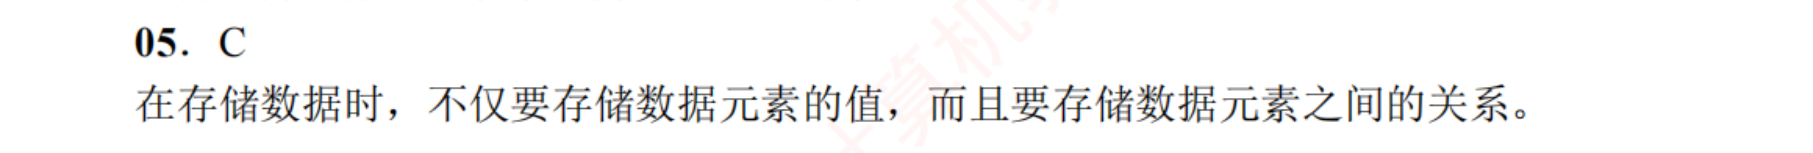
\includegraphics[width=161.13mm,height=180mm,keepaspectratio]{../solutions/assets/04a23d0cdafeff11beaf7d0f.png}\par\smallskip
\par\medskip\Needspace{5\baselineskip}\noindent\hypertarget{a:DS01-E02}{}\label{a:DS01-E02}\textbf{例 1-2}\quad B
\par\smallskip
执行\(k\)轮后，\(sum=k(k+1)/2\)。终止轮数为满足\(k(k+1)/2\ge n\)的最小整数，故\(k=\Theta(\sqrt n)\)；每轮常数时间，选B。

\par\medskip\Needspace{5\baselineskip}\noindent\hypertarget{a:DS01-E03}{}\label{a:DS01-E03}\textbf{例 1-3}\quad B
\par\smallskip
各轮内循环次数为\(1,2,4,\ldots,2^k\)，其中\(2^k<n\le2^{k+1}\)。总次数\(2^{k+1}-1=\Theta(n)\)，选B。

\par\medskip\Needspace{5\baselineskip}\noindent\hypertarget{a:DS01-E04}{}\label{a:DS01-E04}\textbf{例 1-4}\quad B
\par\smallskip
\par\medskip\noindent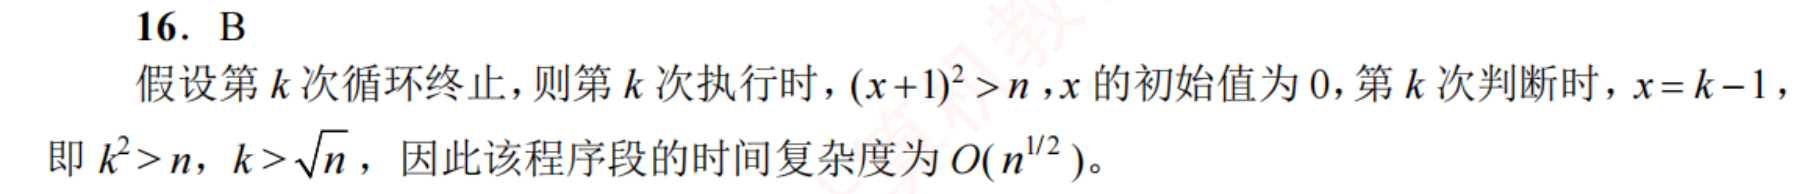
\includegraphics[width=161.13mm,height=180mm,keepaspectratio]{../solutions/assets/3574f5698b4bc0a5ae94a2bb.png}\par\smallskip
\section*{线性表}
\par\medskip\Needspace{5\baselineskip}\noindent\hypertarget{a:DS02-E01}{}\label{a:DS02-E01}\textbf{例 2-1}\quad D
\par\smallskip
\par\medskip\noindent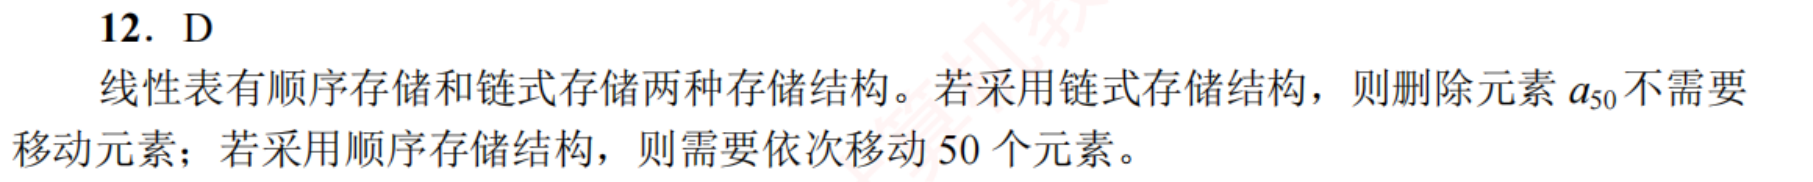
\includegraphics[width=161.13mm,height=180mm,keepaspectratio]{../solutions/assets/aba2847f103acb2776642832.png}\par\smallskip
\par\medskip\Needspace{5\baselineskip}\noindent\hypertarget{a:DS02-E02}{}\label{a:DS02-E02}\textbf{例 2-2}\quad 双指针，时间\(O(n)\)，空间\(O(1)\)
\par\smallskip
倒数位置由尾部决定，但链表不能直接向前访问。让两个指针保持固定间隔：\texttt{fast} 先从首元结点前进 \(k\) 步，再让 \texttt{fast} 与 \texttt{slow} 同步前进。若表长为 \(n\)，\texttt{fast} 到达空位置时共走了 \(n\) 步，\texttt{slow} 只走了 \(n-k\) 步，正好指向第 \(n-k+1\) 个结点。

\begin{codeblock}[language={}]
int searchK(LNode *list, int k) {
    if (k<=0) return 0;
    LNode *fast=list->next, *slow=list->next;
    for (int j=0; j<k; ++j) {
        if (fast==NULL) return 0;   // 表长不足 k
        fast=fast->next;
    }
    while (fast!=NULL) {
        fast=fast->next;
        slow=slow->next;
    }
    printf("%d", slow->data);
    return 1;
}
\end{codeblock}

以长度 5、\(k=2\) 为例，先让 \texttt{fast} 指向第3个结点，\texttt{slow} 留在第1个；同步经过``4与2---5与3---空与4''，第4个即倒数第2个。\(k=n\) 时第一阶段恰好走到空位置，第二阶段不执行，返回首元结点；\(k>n\) 时在第一阶段报失败。两个指针合计走 \(O(n)\) 步，辅助空间 \(O(1)\)，没有修改任何链接。

\par\medskip\Needspace{5\baselineskip}\noindent\hypertarget{a:DS02-E03}{}\label{a:DS02-E03}\textbf{例 2-3}\quad D
\par\smallskip
\par\medskip\noindent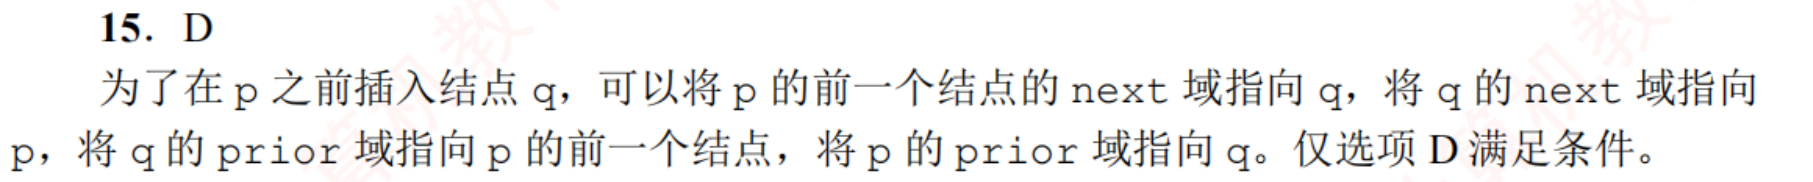
\includegraphics[width=161.13mm,height=180mm,keepaspectratio]{../solutions/assets/57909bf392bf67bc5ac4949d.png}\par\smallskip
\par\medskip\Needspace{5\baselineskip}\noindent\hypertarget{a:DS02-E04}{}\label{a:DS02-E04}\textbf{例 2-4}\quad 三次逆置，时间\(O(n)\)，空间\(O(1)\)
\par\smallskip
题目要求两个连续区段交换位置，同时保持各段内部次序。设前 \(p\) 个元素为 \(A\)，其余为 \(B\)。分别逆置得 \(A^RB^R\)，再整体逆置，即得 \(BA\)。两个区段各被逆置两次，内部方向恢复，而相对位置交换。

\begin{codeblock}[language={}]
void reverse(int R[], int l, int r) {
    while (l<r) {
        int t=R[l]; R[l]=R[r]; R[r]=t;
        ++l; --r;
    }
}
void rotateLeft(int R[], int n, int p) {
    reverse(R,0,p-1);
    reverse(R,p,n-1);
    reverse(R,0,n-1);
}
\end{codeblock}

例如 \texttt{abcdefgh} 左移3位，依次得到 \texttt{cbadefgh}、\texttt{cbahgfed}、\texttt{defghabc}。总交换次数不超过 \(n\)，时间 \(O(n)\)；只用常数临时变量，空间 \(O(1)\)。若将首元素移到末尾重复 \(p\) 次，时间为 \(O(np)\)，当 \(p\) 与 \(n\) 同阶时会退化。三次逆置可处理 \(p=1\) 和 \(p=n-1\)，无需另写搬移循环。

\par\medskip\Needspace{5\baselineskip}\noindent\hypertarget{a:DS02-E05}{}\label{a:DS02-E05}\textbf{例 2-5}\quad 对齐表尾后同步比较地址，时间\(O(m+n)\)
\par\smallskip
共享指的是地址相同，不能以 \texttt{p-\textgreater{}data==q-\textgreater{}data} 判断。单链表一旦在某结点汇合，其后继也相同，所以两表从公共起点到末尾的长度相等。先各扫描一次求长 \(m,n\)，让较长表先走 \(|m-n|\) 步，两指针便处于距表尾相同的位置；此后同步前进，第一次地址相等的位置就是答案。

\begin{codeblock}[language={}]
LNode *commonSuffix(LNode *str1, LNode *str2) {
    int m=0,n=0;
    for (LNode *p=str1->next; p; p=p->next) ++m;
    for (LNode *q=str2->next; q; q=q->next) ++n;
    LNode *p=str1->next, *q=str2->next;
    while (m>n) { p=p->next; --m; }
    while (n>m) { q=q->next; --n; }
    while (p!=q) { p=p->next; q=q->next; }
    return p;                   // 无公共结点时二者同时为 NULL
}
\end{codeblock}

图中两表长度分别为7和5，先让长表跨过 \texttt{l,o}，再比较 \texttt{a} 与 \texttt{b}、\texttt{d} 与 \texttt{e}，最后到达同一个 \texttt{i}。若两表内容相同却各自分配结点，则直到空位置才相等，返回空。总时间 \(O(m+n)\)，辅助空间 \(O(1)\)，适用于有限、无环单链表。

\par\medskip\Needspace{5\baselineskip}\noindent\hypertarget{a:DS02-E06}{}\label{a:DS02-E06}\textbf{例 2-6}\quad 抵消候选后再次计数，时间\(O(n)\)，空间\(O(1)\)
\par\smallskip
每次删除两个值不同的元素，不会消灭一个原本占严格多数的值：若删去一个多数元素和一个其他元素，多数仍超过剩余的一半；若删去两个其他元素，多数优势更大。用一个候选值和计数模拟这种抵消。计数为0时选新候选；相同则加1，不同则减1。

\begin{codeblock}[language={}]
int majority(int A[], int n) {
    int candidate=0, count=0;
    for (int i=0; i<n; ++i) {
        if (count==0) { candidate=A[i]; count=1; }
        else if (A[i]==candidate) ++count;
        else --count;
    }
    int actual=0;
    for (int i=0; i<n; ++i)
        if (A[i]==candidate) ++actual;
    return actual>n/2 ? candidate : -1;
}
\end{codeblock}

抵消只保证``若有主元素，最后候选一定是它''，没有保证主元素存在。例如 \texttt{1,2,3} 最后仍可能留下候选3，它只出现一次，所以必须第二次扫描核实。两个线性扫描合计 \(O(n)\) 时间，额外空间 \(O(1)\)。题目给出的值域也允许用计数数组，但需 \(O(n)\) 辅助空间；此处没有必要为省下一次扫描而付出这部分空间。

\section*{栈、队列和数组}
\par\medskip\Needspace{5\baselineskip}\noindent\hypertarget{a:DS03-E01}{}\label{a:DS03-E01}\textbf{例 3-1}\quad C
\par\smallskip
\par\medskip\noindent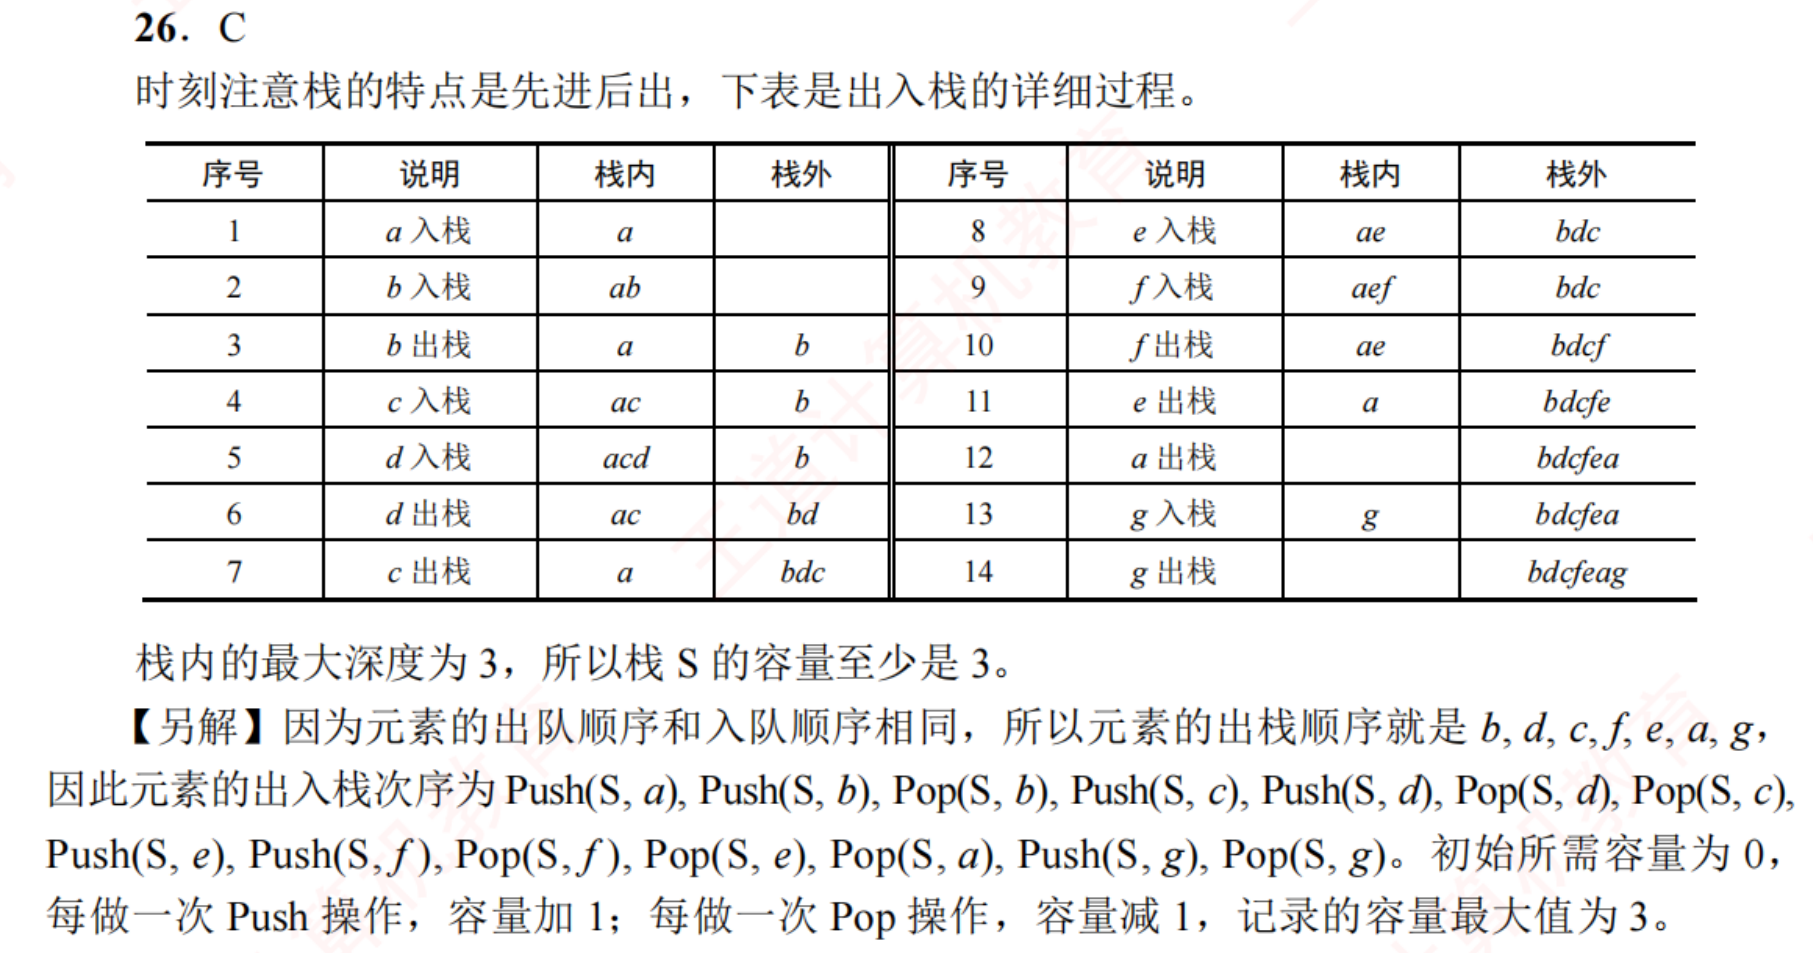
\includegraphics[width=161.13mm,height=180mm,keepaspectratio]{../solutions/assets/31eb8d5541108602e1720deb.png}\par\smallskip
\par\medskip\Needspace{5\baselineskip}\noindent\hypertarget{a:DS03-E02}{}\label{a:DS03-E02}\textbf{例 3-2}\quad C
\par\smallskip
\par\medskip\noindent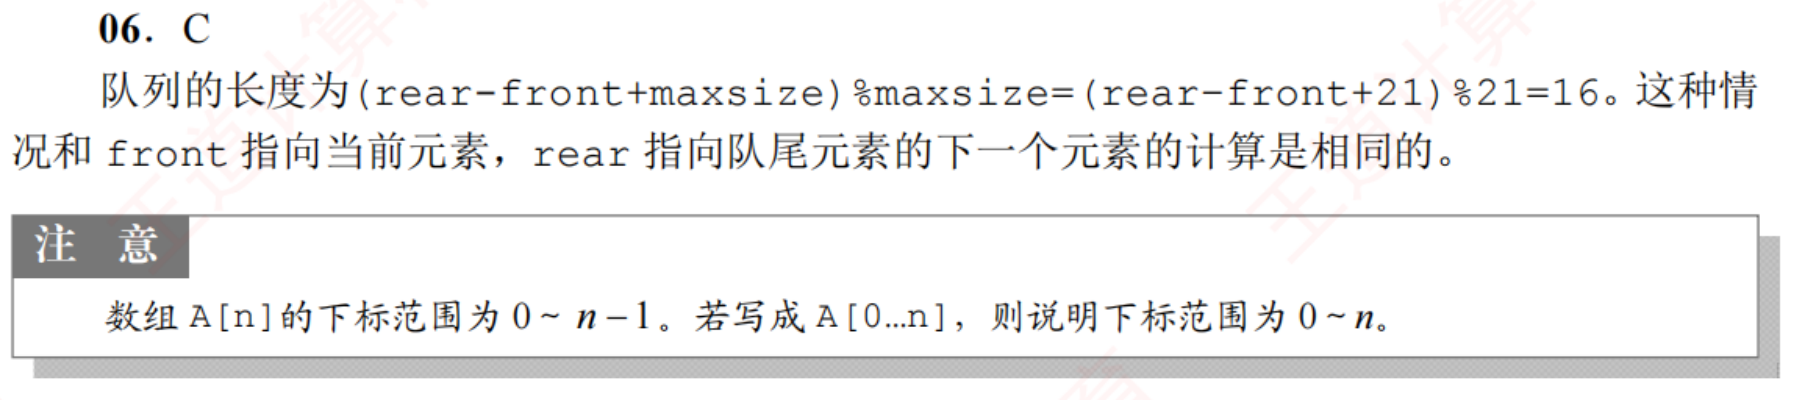
\includegraphics[width=161.13mm,height=180mm,keepaspectratio]{../solutions/assets/24d529bbe1b7eee11064ad2d.png}\par\smallskip
\par\medskip\Needspace{5\baselineskip}\noindent\hypertarget{a:DS03-E03}{}\label{a:DS03-E03}\textbf{例 3-3}\quad B
\par\smallskip
\par\medskip\noindent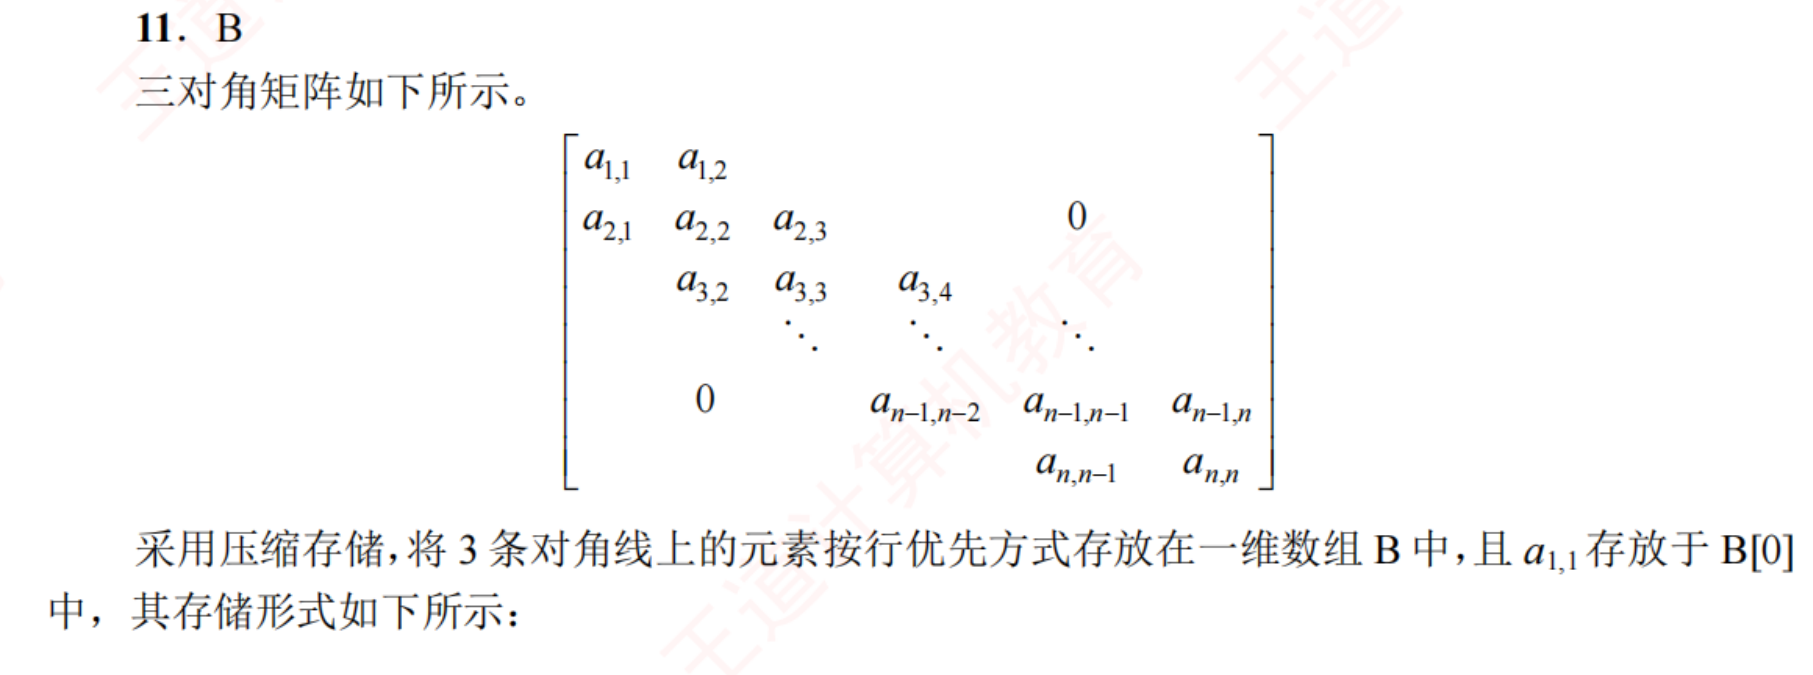
\includegraphics[width=161.13mm,height=180mm,keepaspectratio]{../solutions/assets/d902369097e4259bb9d03cde.png}\par\smallskip
\par\medskip\noindent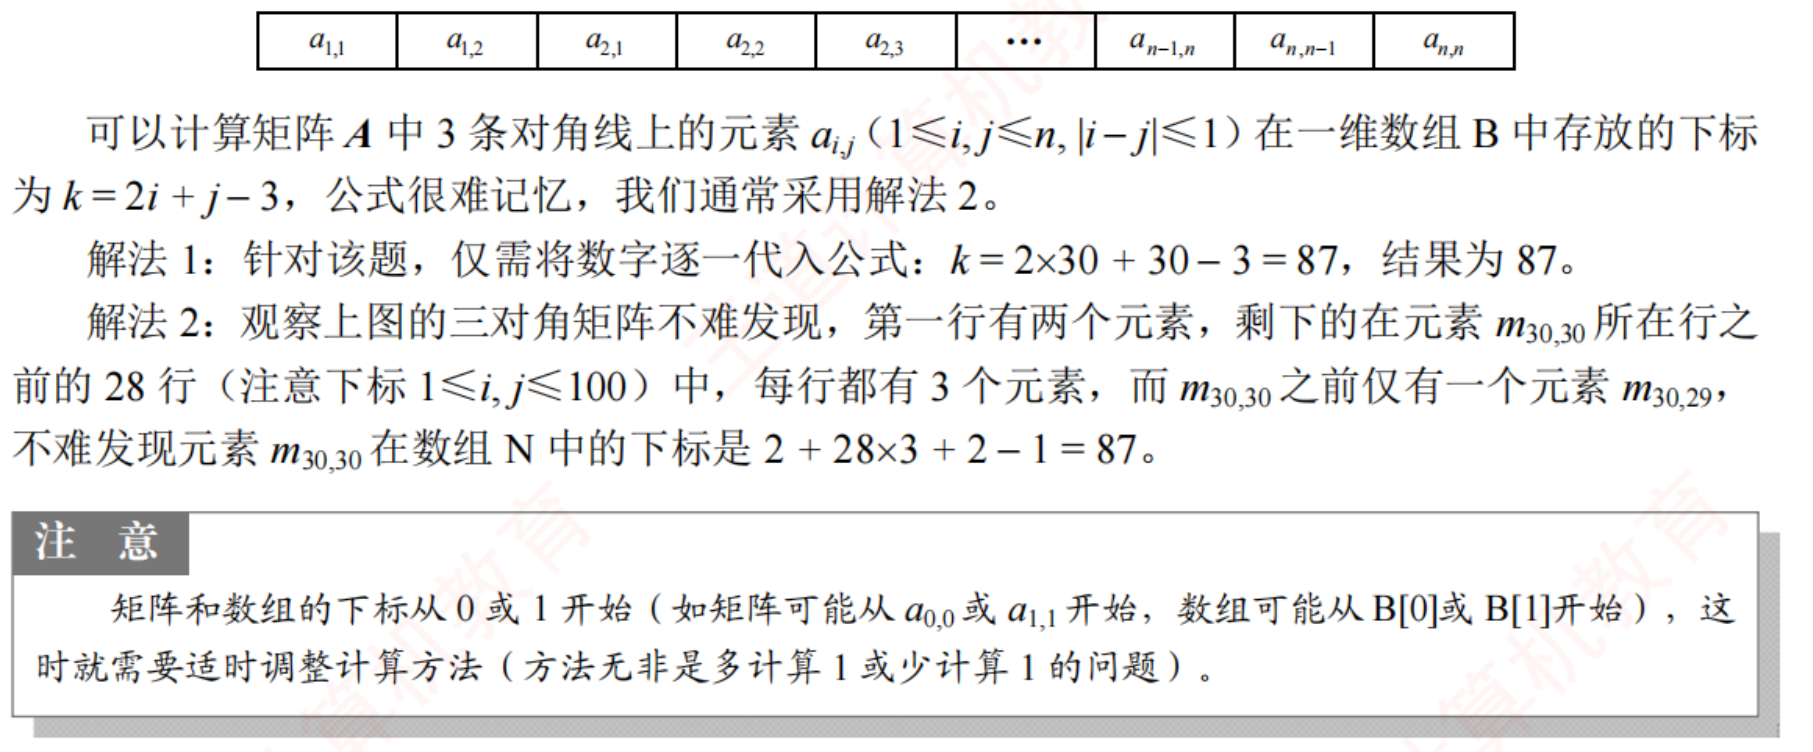
\includegraphics[width=161.13mm,height=180mm,keepaspectratio]{../solutions/assets/bb2681687be7e02522d0920d.png}\par\smallskip
\par\medskip\Needspace{5\baselineskip}\noindent\hypertarget{a:DS03-E04}{}\label{a:DS03-E04}\textbf{例 3-4}\quad C
\par\smallskip
\par\medskip\noindent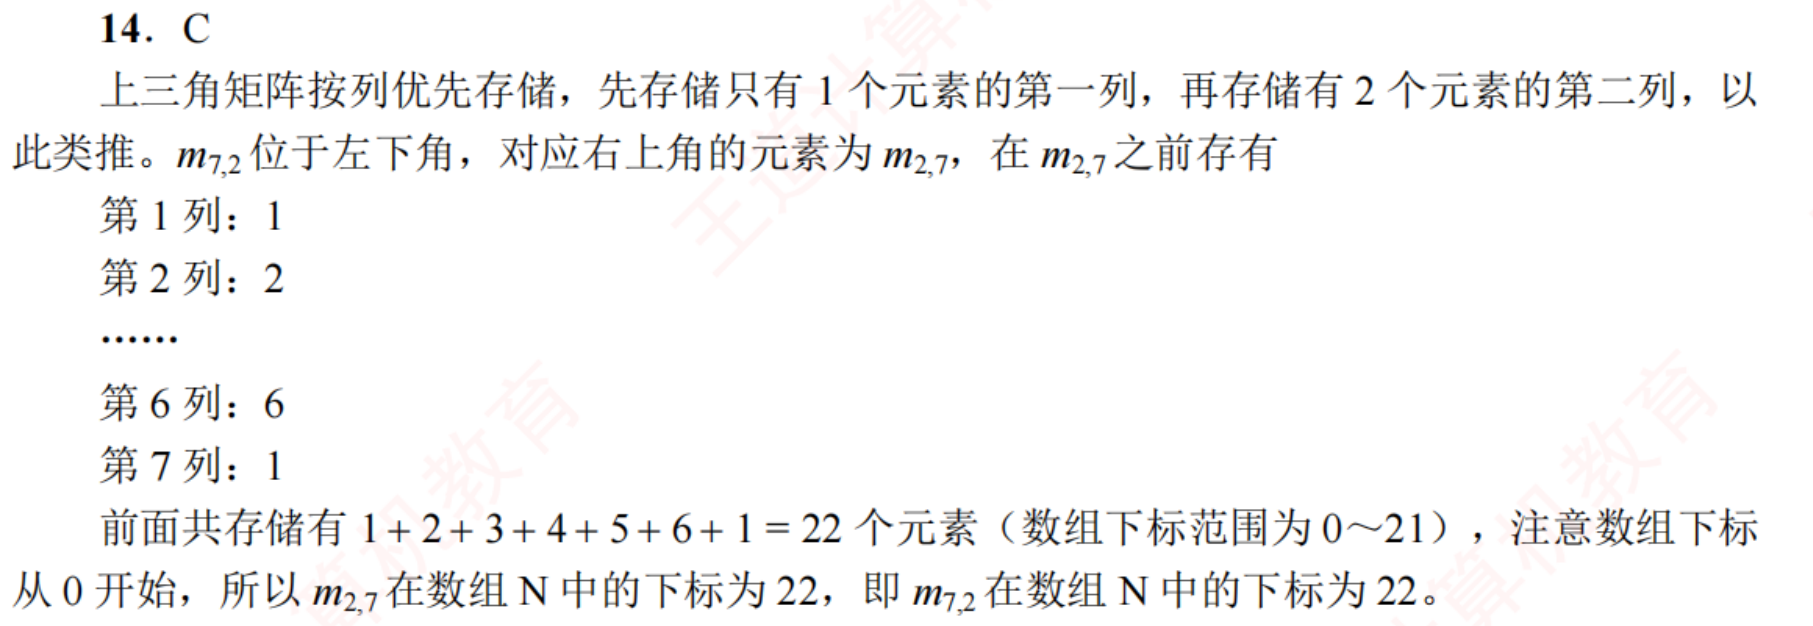
\includegraphics[width=161.13mm,height=180mm,keepaspectratio]{../solutions/assets/72ca9acbba6a3cf8e2d07ad3.png}\par\smallskip
\par\medskip\Needspace{5\baselineskip}\noindent\hypertarget{a:DS03-E05}{}\label{a:DS03-E05}\textbf{例 3-5}\quad B
\par\smallskip
\par\medskip\noindent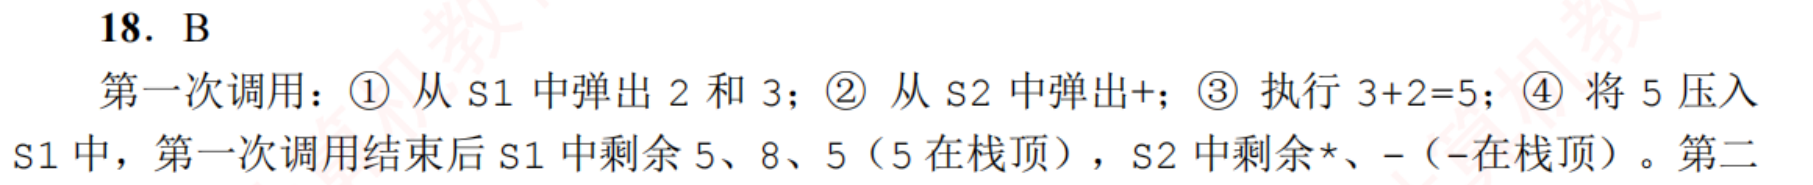
\includegraphics[width=161.13mm,height=180mm,keepaspectratio]{../solutions/assets/0af1233cf2f111913104813d.png}\par\smallskip
\par\medskip\noindent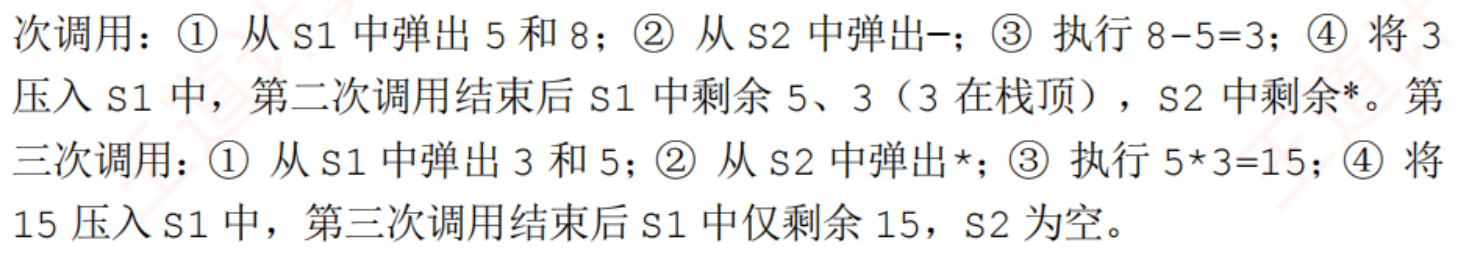
\includegraphics[width=129.65mm,height=180mm,keepaspectratio]{../solutions/assets/e9cc980f15dafe85c14a44e4.png}\par\smallskip
\section*{串}
\par\medskip\Needspace{5\baselineskip}\noindent\hypertarget{a:DS04-E01}{}\label{a:DS04-E01}\textbf{例 4-1}\quad 位置均为4；朴素15次，普通KMP10次
\par\smallskip
朴素匹配从起点1、2、3、4依次比较6、1、2、6次，共15次。普通next为\texttt{0,1,1,2,2,3}；KMP前5对相等，第6对在\texttt{(i,j)=(6,6)}失配，令\texttt{j=3}、\texttt{i}保持6；随后\texttt{(6,3)、(7,4)、(8,5)、(9,6)}均相等，共10次字符比较，返回\texttt{10-6=4}。

\par\medskip\Needspace{5\baselineskip}\noindent\hypertarget{a:DS04-E02}{}\label{a:DS04-E02}\textbf{例 4-2}\quad 位置5；普通next比较12次，nextval比较9次
\par\smallskip
普通next为\texttt{0,1,2,3,4}，nextval为\texttt{0,0,0,0,4}。前3对\texttt{a}相等；主串第4位\texttt{c}在普通表下依次与模式第4、3、2、1位失配，优化表在第一次失配后直接退到0。推进到主串第5位后，连续匹配\texttt{aaaab}。普通表比较\texttt{3+4+5=12}次，优化表比较\texttt{3+1+5=9}次，均返回5。

\section*{树与二叉树}
\par\medskip\Needspace{5\baselineskip}\noindent\hypertarget{a:DS05-E01}{}\label{a:DS05-E01}\textbf{例 5-1}\quad B
\par\smallskip
\par\medskip\noindent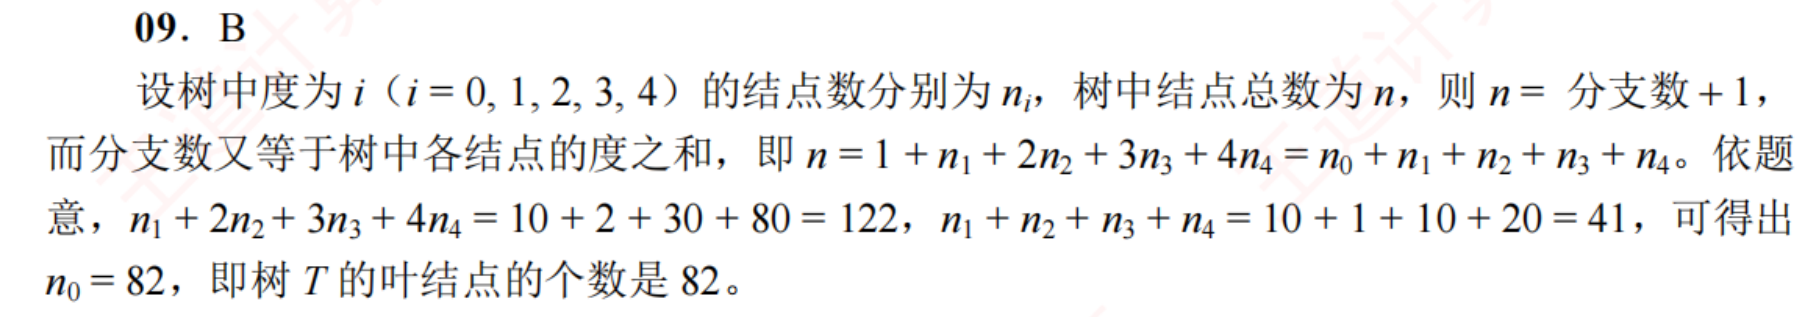
\includegraphics[width=161.13mm,height=180mm,keepaspectratio]{../solutions/assets/2f778ee5c018996463e9b202.png}\par\smallskip
\par\medskip\Needspace{5\baselineskip}\noindent\hypertarget{a:DS05-E02}{}\label{a:DS05-E02}\textbf{例 5-2}\quad A
\par\smallskip
\par\medskip\noindent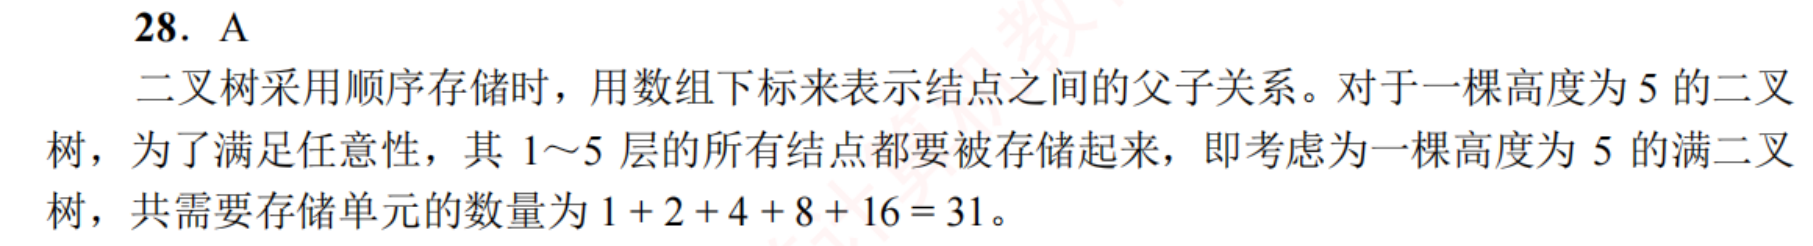
\includegraphics[width=161.13mm,height=180mm,keepaspectratio]{../solutions/assets/f3ad9320a6af8b68276d3dc2.png}\par\smallskip
\par\medskip\Needspace{5\baselineskip}\noindent\hypertarget{a:DS05-E03}{}\label{a:DS05-E03}\textbf{例 5-3}\quad A
\par\smallskip
\par\medskip\noindent
\includegraphics[width=130.02mm,height=180mm,keepaspectratio]{../solutions/assets/9481744cb129c6e8ff820dca.png}\par\smallskip
\par\medskip\noindent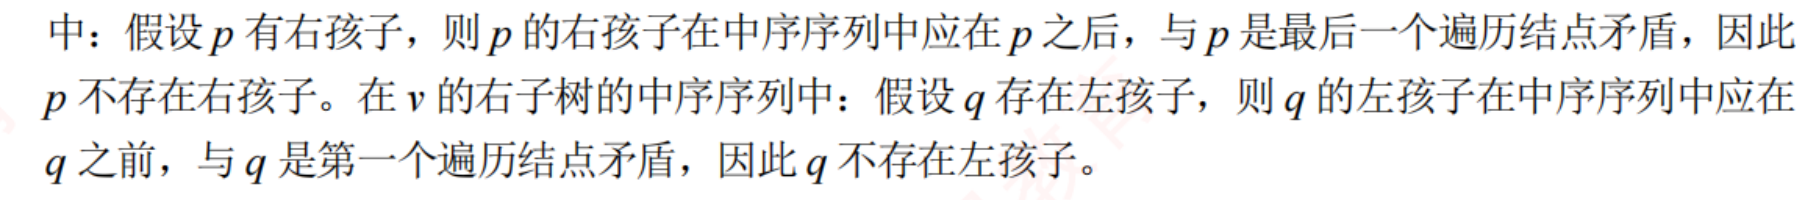
\includegraphics[width=161.13mm,height=180mm,keepaspectratio]{../solutions/assets/2044e5c6e7ee926641dbf9fa.png}\par\smallskip
\par\medskip\Needspace{5\baselineskip}\noindent\hypertarget{a:DS05-E04}{}\label{a:DS05-E04}\textbf{例 5-4}\quad B
\par\smallskip
\par\medskip\noindent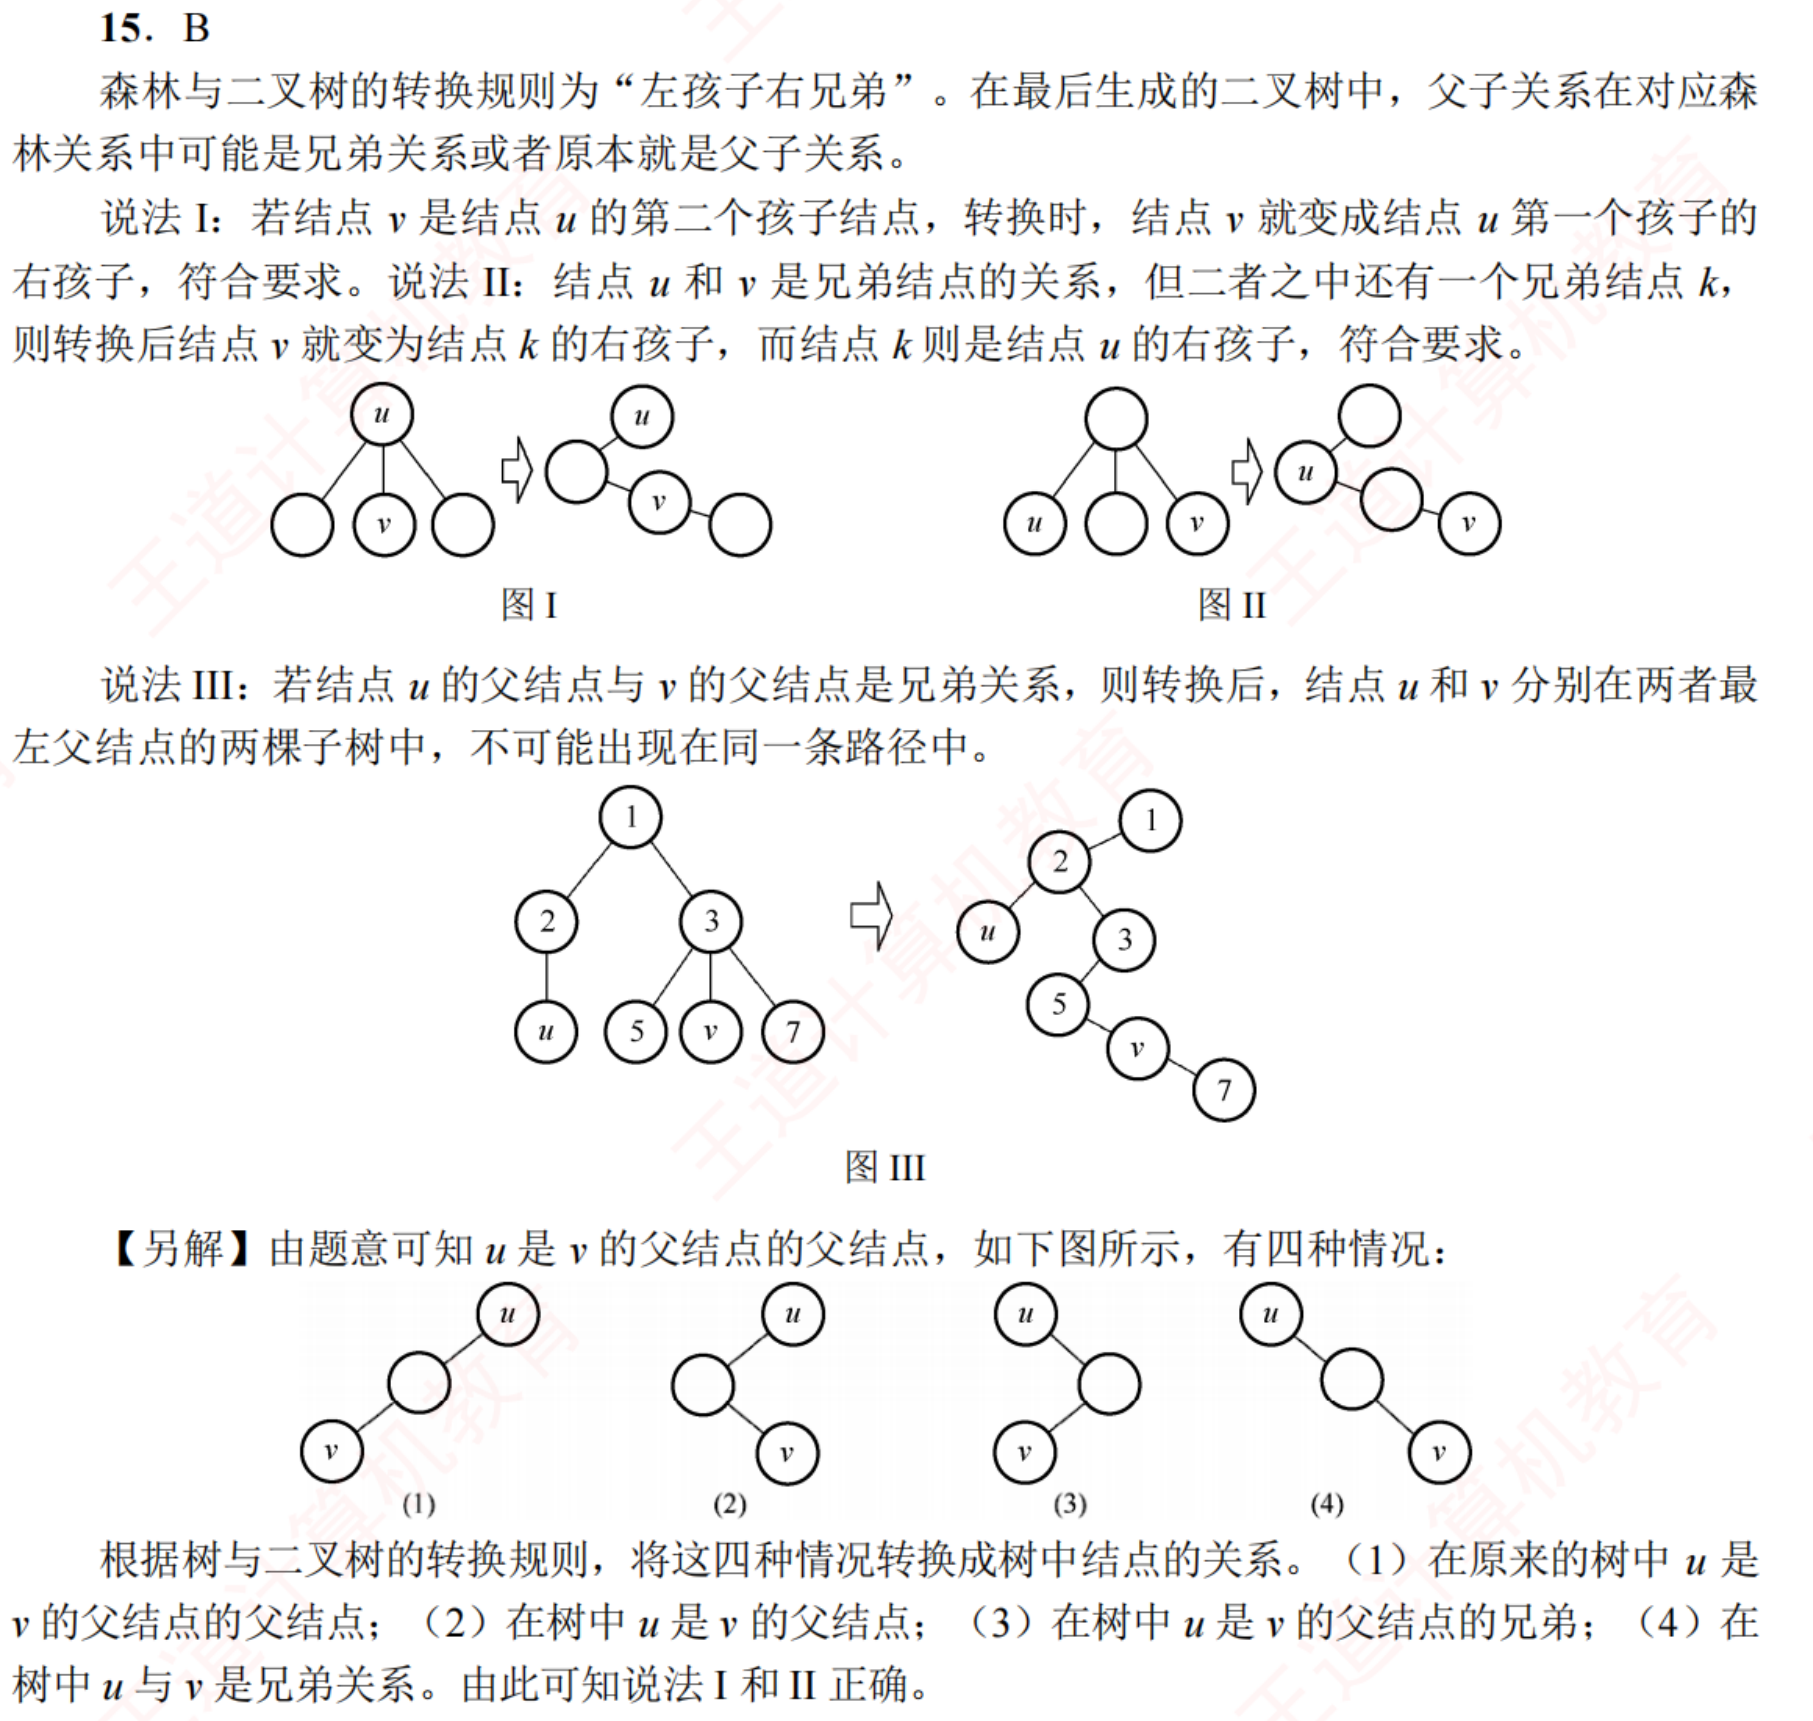
\includegraphics[width=161.13mm,height=180mm,keepaspectratio]{../solutions/assets/448d8500b3d17a7583a274a0.png}\par\smallskip
\par\medskip\Needspace{5\baselineskip}\noindent\hypertarget{a:DS05-E05}{}\label{a:DS05-E05}\textbf{例 5-5}\quad B
\par\smallskip
\par\medskip\noindent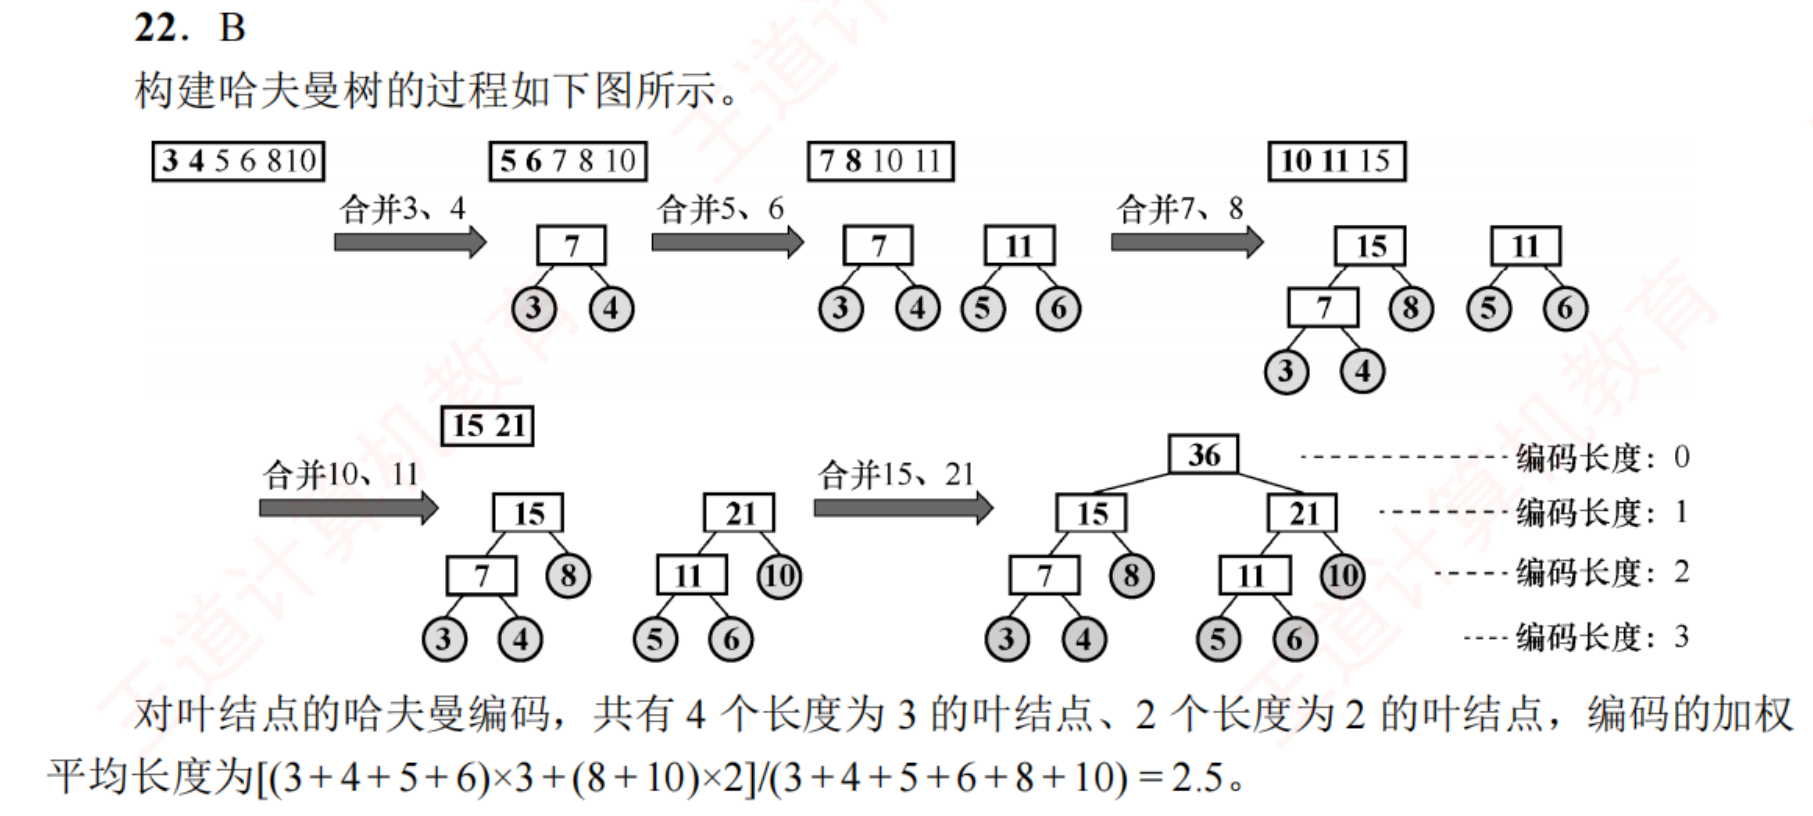
\includegraphics[width=161.13mm,height=180mm,keepaspectratio]{../solutions/assets/e0c6a8726b4dfd758fbce6c2.png}\par\smallskip
\par\medskip\Needspace{5\baselineskip}\noindent\hypertarget{a:DS05-E06}{}\label{a:DS05-E06}\textbf{例 5-6}\quad C
\par\smallskip
\par\medskip\noindent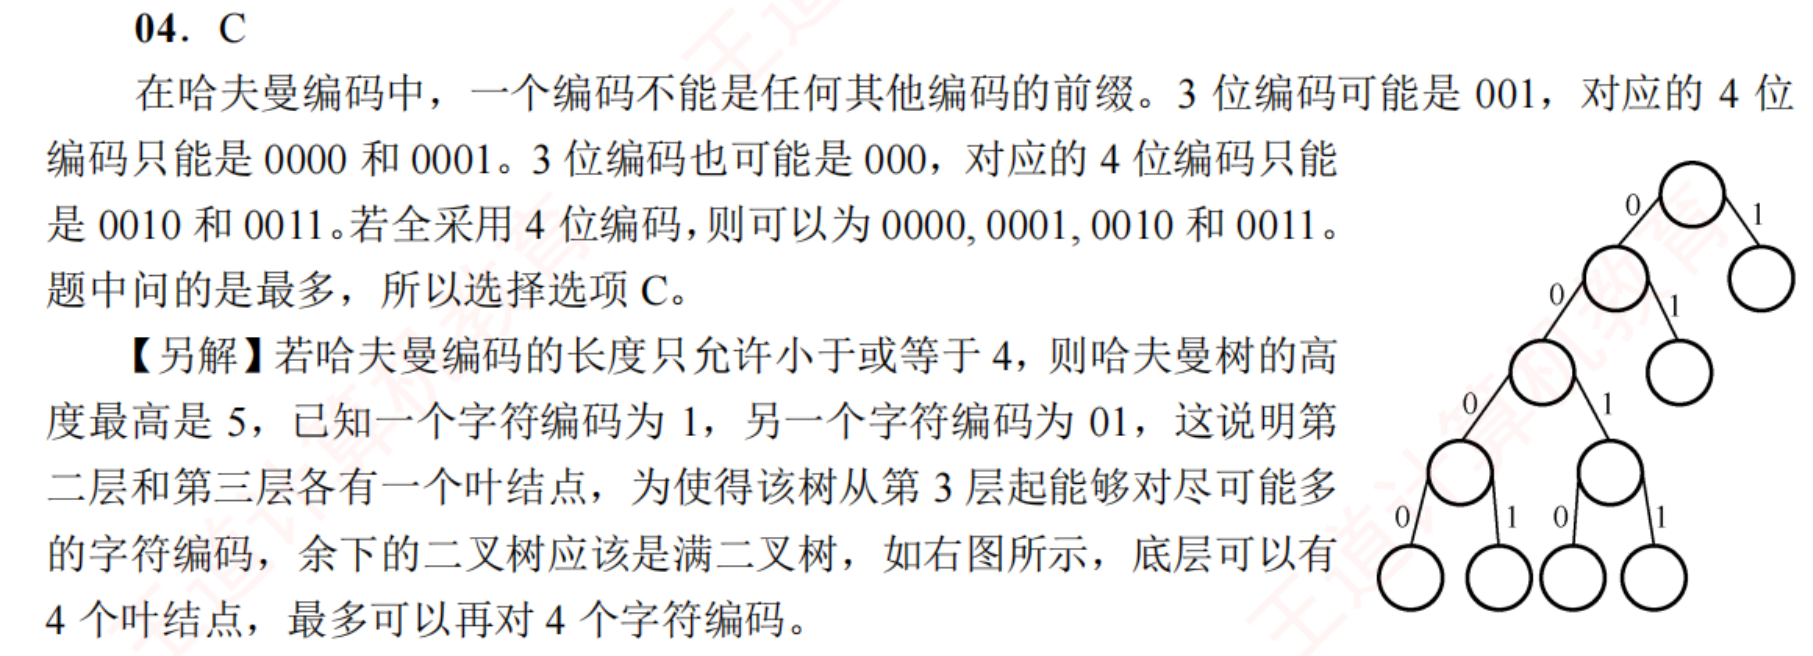
\includegraphics[width=161.13mm,height=180mm,keepaspectratio]{../solutions/assets/eacc638d7b0b75902184126f.png}\par\smallskip
\section*{图}
\par\medskip\Needspace{5\baselineskip}\noindent\hypertarget{a:DS06-E01}{}\label{a:DS06-E01}\textbf{例 6-1}\quad C
\par\smallskip
\par\medskip\noindent
\includegraphics[width=161.13mm,height=180mm,keepaspectratio]{../solutions/assets/a6ebaca181170a035fdd0b18.png}\par\smallskip
\par\medskip\noindent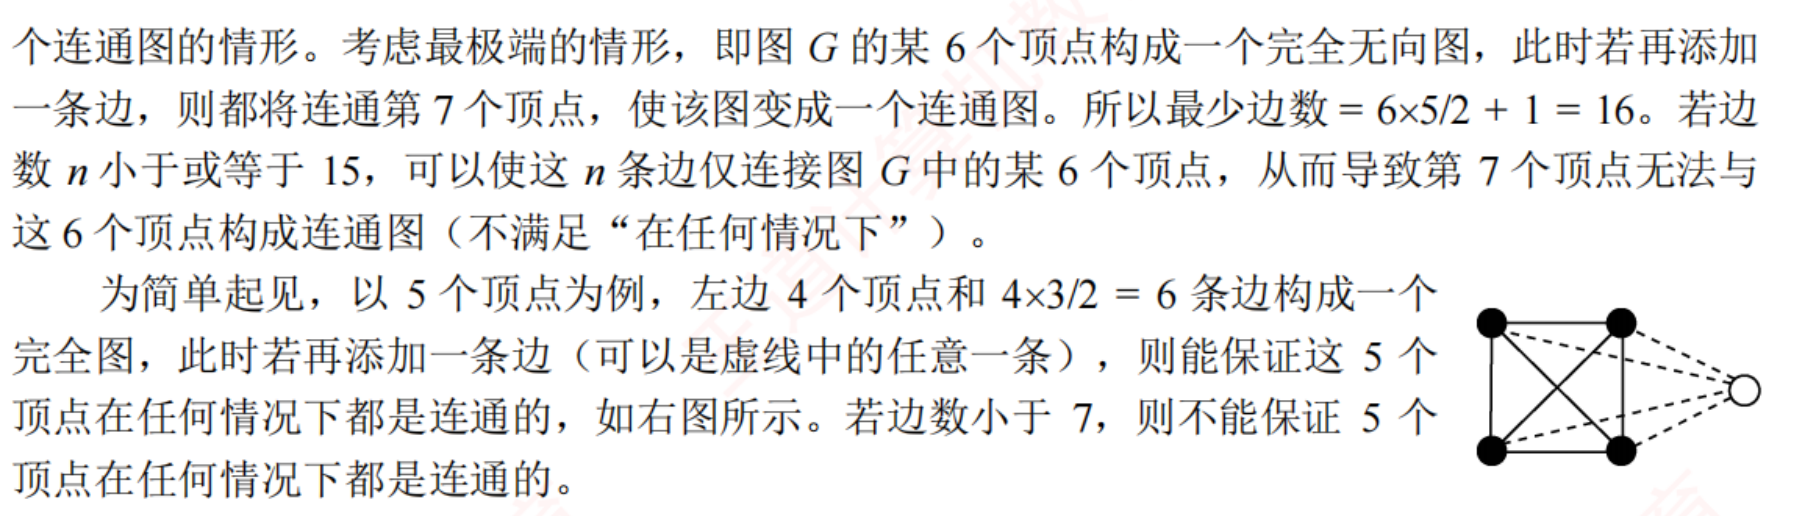
\includegraphics[width=161.13mm,height=180mm,keepaspectratio]{../solutions/assets/8a706a4a9a396bb57de7600a.png}\par\smallskip
\par\medskip\Needspace{5\baselineskip}\noindent\hypertarget{a:DS06-E02}{}\label{a:DS06-E02}\textbf{例 6-2}\quad D
\par\smallskip
\par\medskip\noindent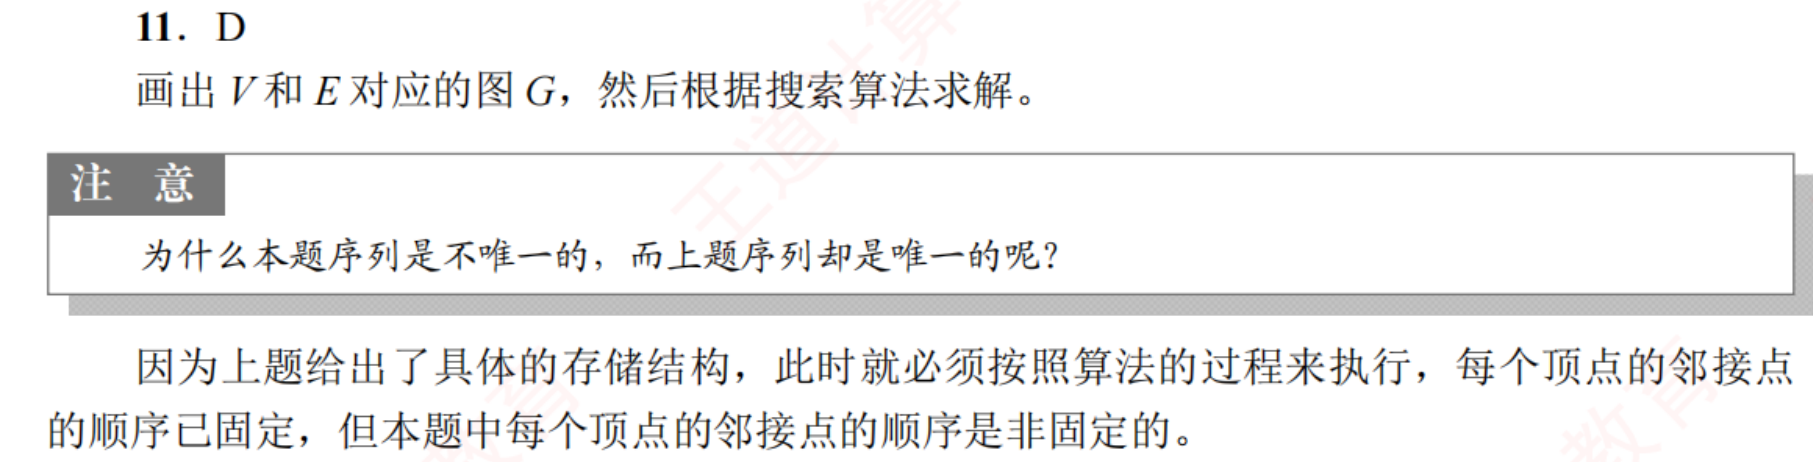
\includegraphics[width=161.13mm,height=180mm,keepaspectratio]{../solutions/assets/802d6c403363ea6ddcd7e28d.png}\par\smallskip
\par\medskip\Needspace{5\baselineskip}\noindent\hypertarget{a:DS06-E03}{}\label{a:DS06-E03}\textbf{例 6-3}\quad C
\par\smallskip
两者首先选权5的\((V_1,V_4)\)。Kruskal第2条可取不成环的任一权8边，包括\((V_2,V_3)\)。Prim此时集合为\(\{V_1,V_4\}\)，只能选跨割边\((V_1,V_3)\)或\((V_4,V_3)\)，选C。

\par\medskip\Needspace{5\baselineskip}\noindent\hypertarget{a:DS06-E04}{}\label{a:DS06-E04}\textbf{例 6-4}\quad C
\par\smallskip
起点确定后初始向量为\((26,3,\infty,6)\)。先确定3，经3到2得到\(3+22=25\)；再确定5，经5到2得到\(6+15=21\)，经5到4得到\(6+8=14\)，故为\((21,3,14,6)\)，选C。经4把到2改成15属于下一轮。

\par\medskip\Needspace{5\baselineskip}\noindent\hypertarget{a:DS06-E05}{}\label{a:DS06-E05}\textbf{例 6-5}\quad 每轮零入度候选恰有一个，且处理完全体顶点
\par\smallskip
\par\medskip\noindent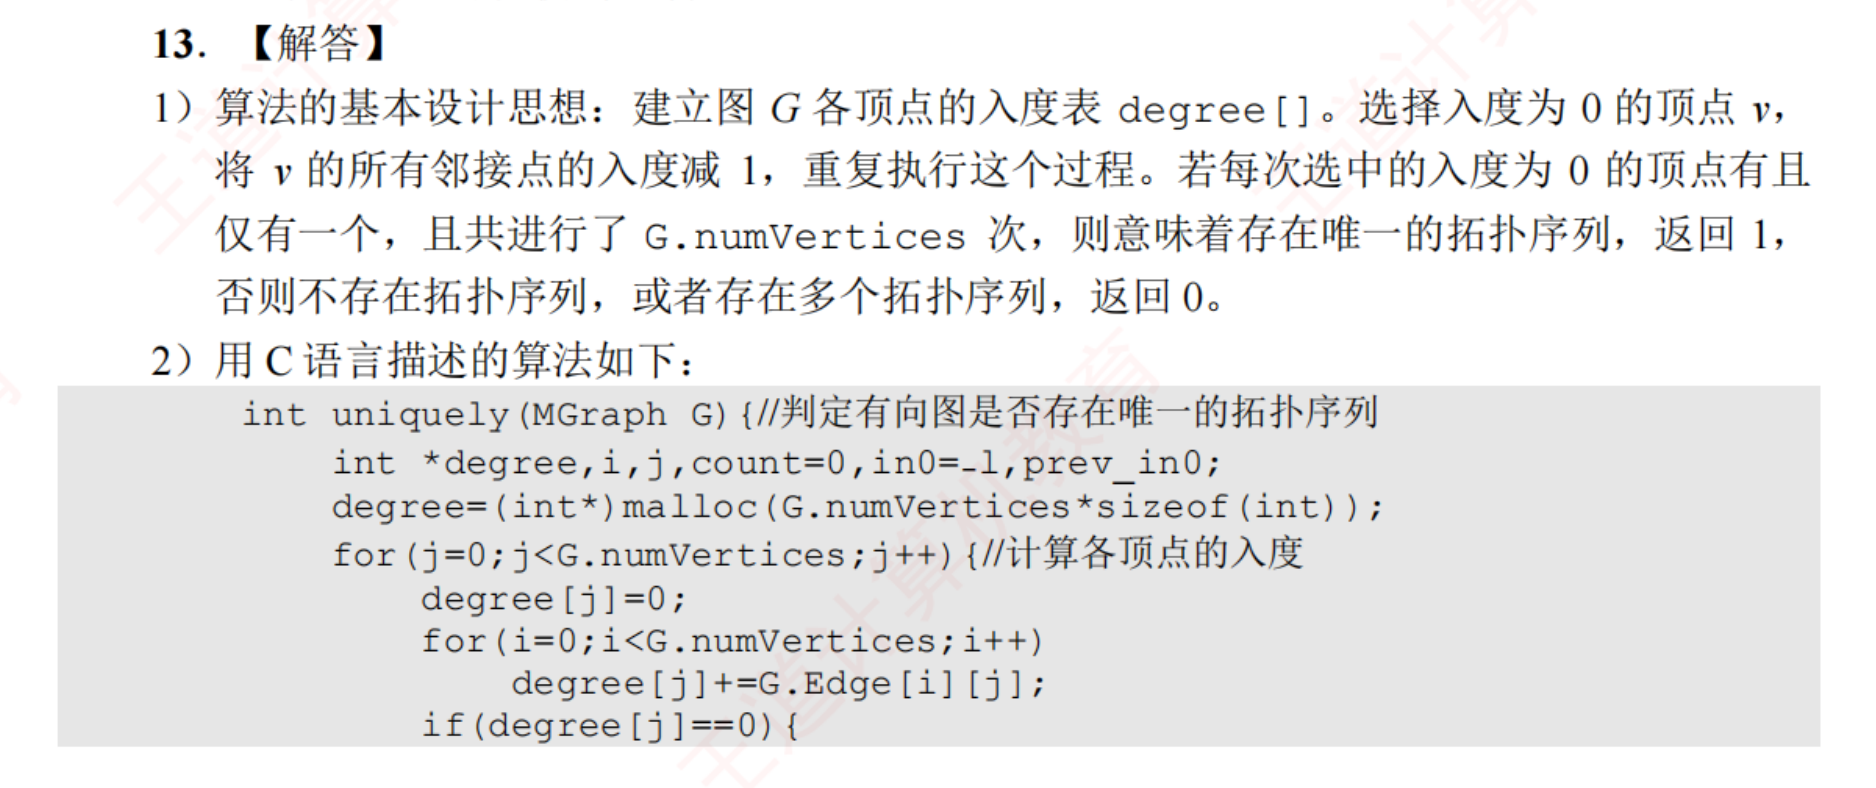
\includegraphics[width=162.00mm,height=180mm,keepaspectratio]{../solutions/assets/15ee3c838a57b152795fe93e.png}\par\smallskip
\par\medskip\noindent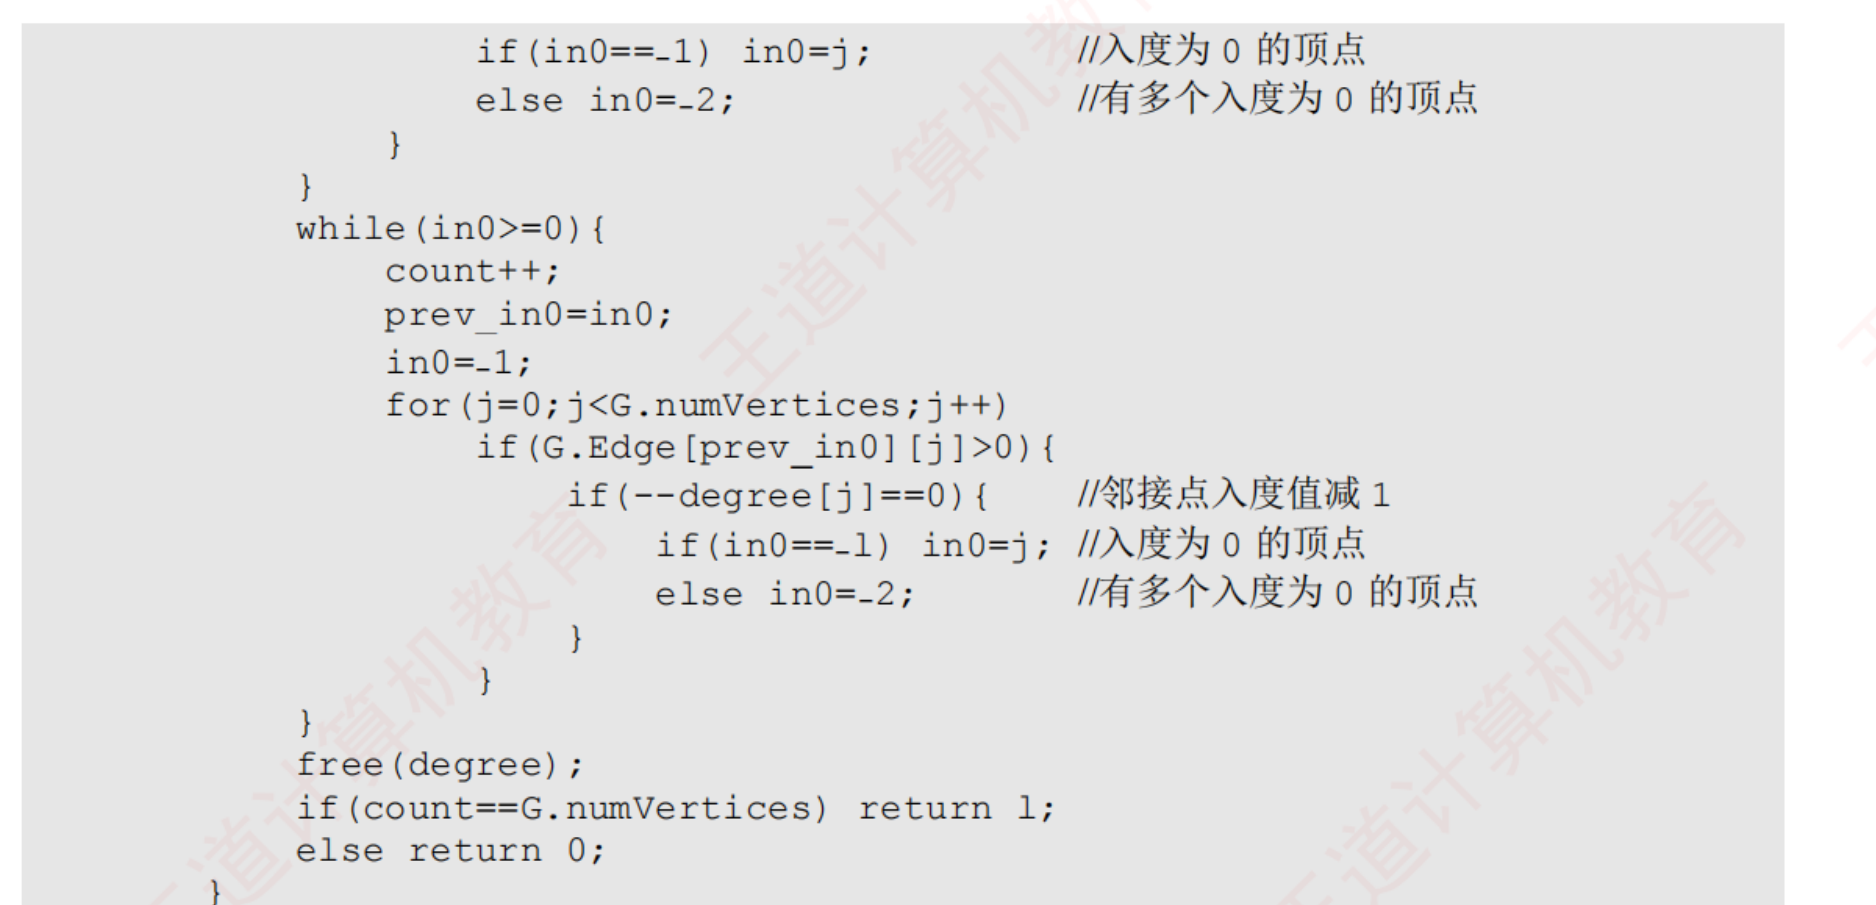
\includegraphics[width=162.00mm,height=180mm,keepaspectratio]{../solutions/assets/a30f3ae056c9de27b5fba7cd.png}\par\smallskip
\par\medskip\Needspace{5\baselineskip}\noindent\hypertarget{a:DS06-E06}{}\label{a:DS06-E06}\textbf{例 6-6}\quad C
\par\smallskip
按拓扑序1、3、2、4、5、6求得事件最早、最迟时间均依次为0、8、12、21、18、27。工期27，关键路径为\texttt{b-d-c-g}、\texttt{b-d-e-h}、\texttt{b-f-h}。同时缩短d、f可覆盖三条关键路径；A、B遗漏\texttt{b-f-h}，D遗漏\texttt{b-d-c-g}，选C。持续缩短后应重算新关键路径。

\section*{查找}
\par\medskip\Needspace{5\baselineskip}\noindent\hypertarget{a:DS07-E01}{}\label{a:DS07-E01}\textbf{例 7-1}\quad C
\par\smallskip
\par\medskip\noindent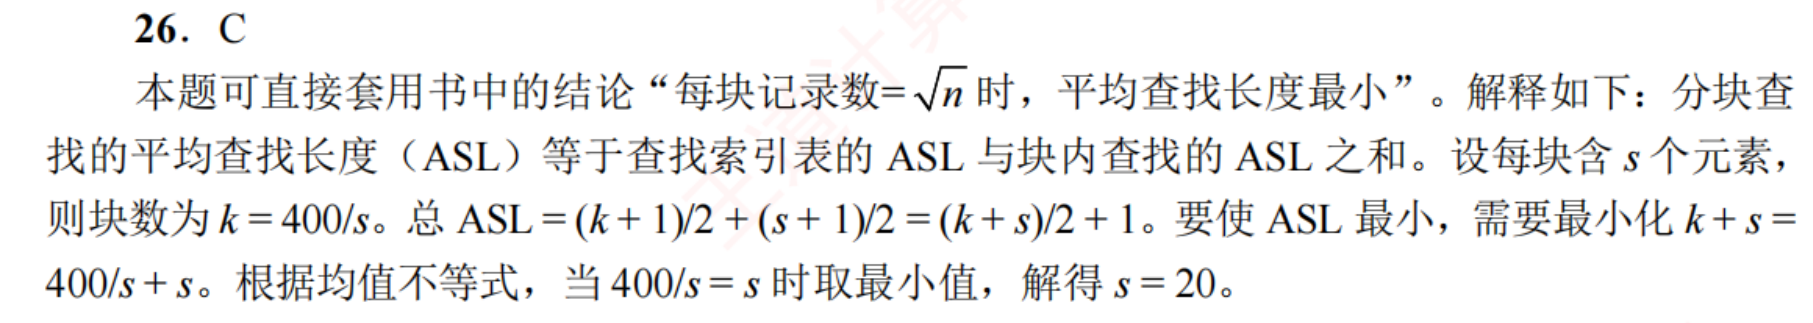
\includegraphics[width=161.13mm,height=180mm,keepaspectratio]{../solutions/assets/244eadb698f738510f77935e.png}\par\smallskip
\par\medskip\Needspace{5\baselineskip}\noindent\hypertarget{a:DS07-E02}{}\label{a:DS07-E02}\textbf{例 7-2}\quad B
\par\smallskip
\par\medskip\noindent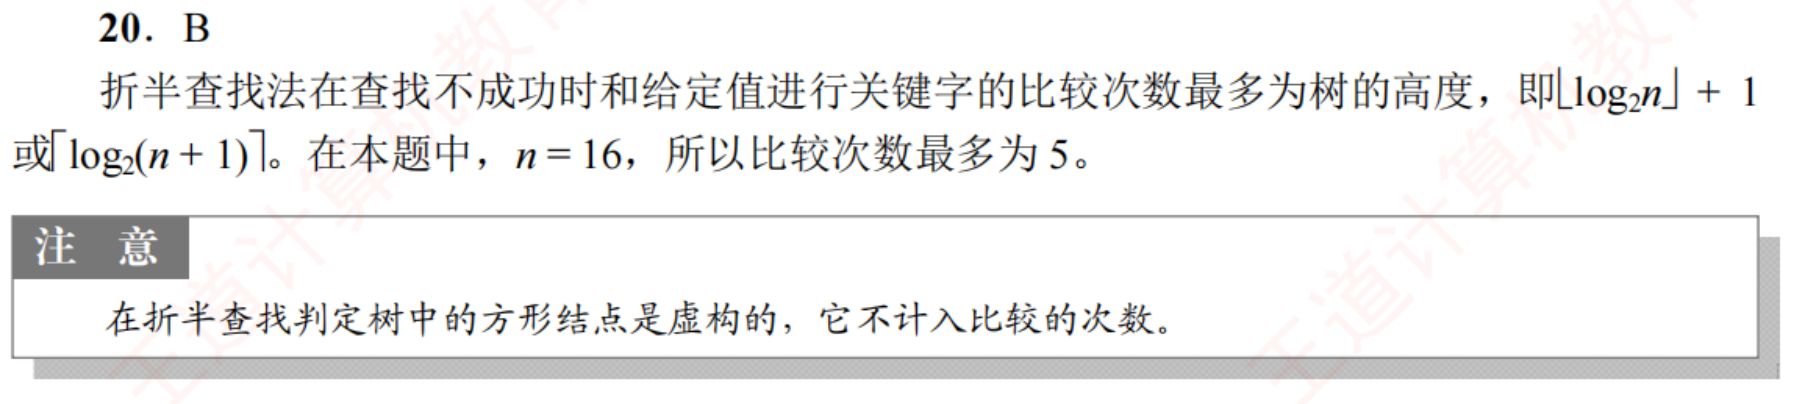
\includegraphics[width=161.13mm,height=180mm,keepaspectratio]{../solutions/assets/09db7cb2daa8a9773f487ab2.png}\par\smallskip
\par\medskip\Needspace{5\baselineskip}\noindent\hypertarget{a:DS07-E03}{}\label{a:DS07-E03}\textbf{例 7-3}\quad 最终为34(23(15,28),107(98,115))
\par\smallskip
以下用 \texttt{根(左子树,右子树)} 表示局部结构，\texttt{∅} 表示空。

\begin{longtable}[]{@{}lll@{}}
\toprule\noalign{}
插入 & 失衡处与调整 & 调整后整树 \\
\midrule\noalign{}
\endhead
\bottomrule\noalign{}
\endlastfoot
34 & 无 & 34 \\
23 & 无 & 34(23,∅) \\
15 & 34处LL，右旋 & 23(15,34) \\
98 & 无 & 23(15,34(∅,98)) \\
115 & 34处RR，左旋 & 23(15,98(34,115)) \\
28 & 23处RL，先右旋98，再左旋23 & 34(23(15,28),98(∅,115)) \\
107 & 98处RL，先右旋115，再左旋98 & 34(23(15,28),107(98,115)) \\
\end{longtable}

插入28时，34仍平衡，最小失衡祖先为23；新增路径为``23的右---98的左''，采用RL。各步中序均为已插入关键字的升序。

\par\medskip\Needspace{5\baselineskip}\noindent\hypertarget{a:DS07-E04}{}\label{a:DS07-E04}\textbf{例 7-4}\quad D
\par\smallskip
\par\medskip\noindent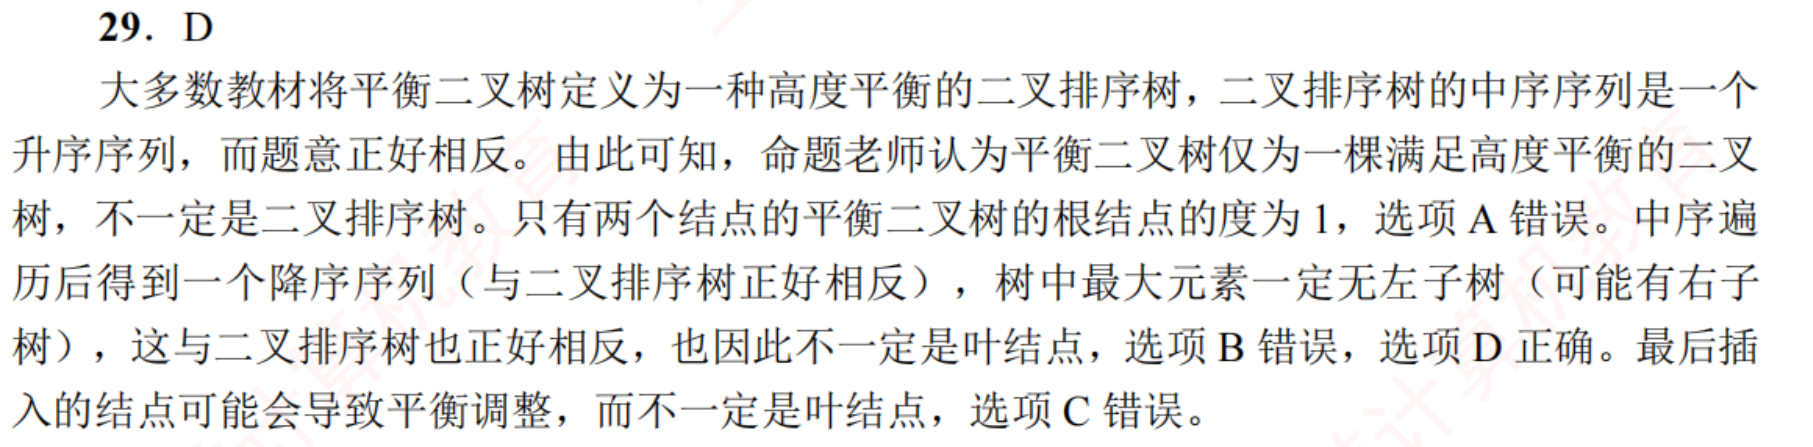
\includegraphics[width=161.13mm,height=180mm,keepaspectratio]{../solutions/assets/f8b3cb6a3068b238f53c7a80.png}\par\smallskip
\par\medskip\Needspace{5\baselineskip}\noindent\hypertarget{a:DS07-E05}{}\label{a:DS07-E05}\textbf{例 7-5}\quad A、D
\par\smallskip
\par\medskip\noindent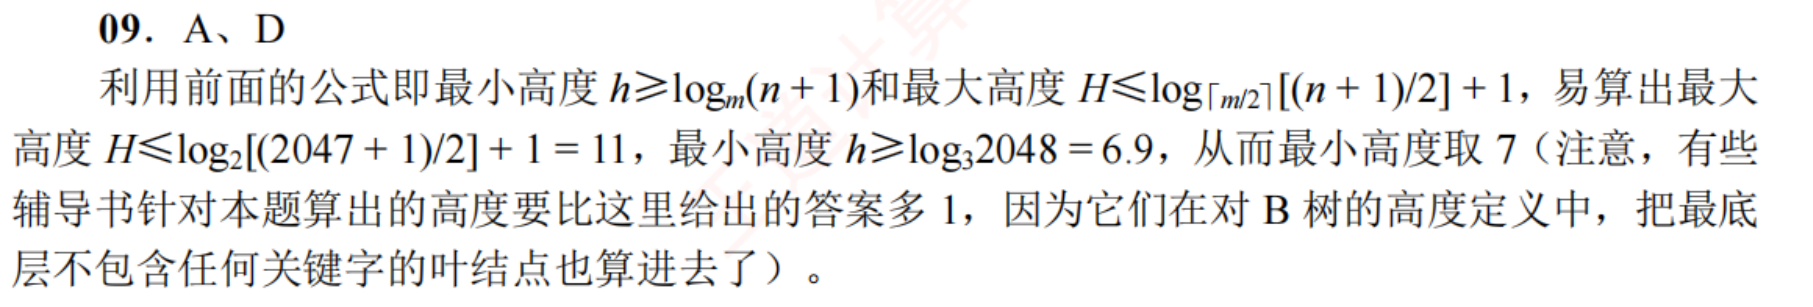
\includegraphics[width=161.13mm,height=180mm,keepaspectratio]{../solutions/assets/0070f8b1bc17ec1f57aa4e6a.png}\par\smallskip
\par\medskip\Needspace{5\baselineskip}\noindent\hypertarget{a:DS07-E06}{}\label{a:DS07-E06}\textbf{例 7-6}\quad C
\par\smallskip
\par\medskip\noindent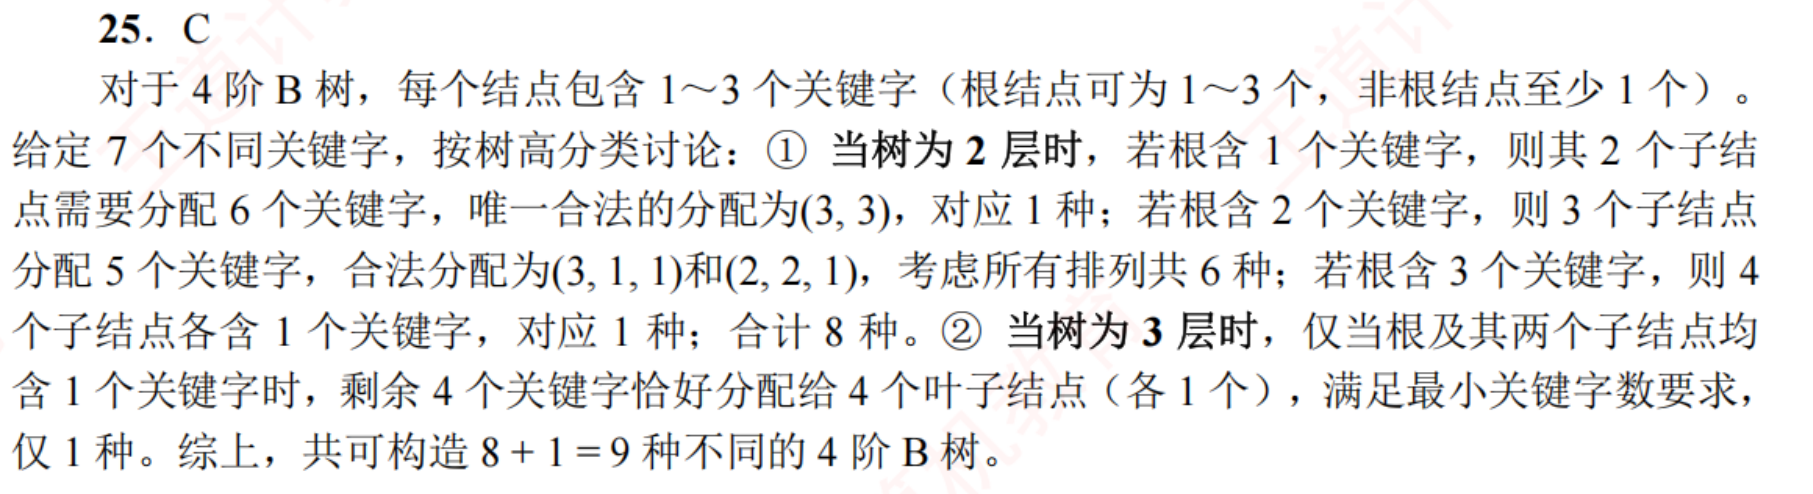
\includegraphics[width=161.13mm,height=180mm,keepaspectratio]{../solutions/assets/ad2673b2dba680f9288d4ac2.png}\par\smallskip
\par\medskip\Needspace{5\baselineskip}\noindent\hypertarget{a:DS07-E07}{}\label{a:DS07-E07}\textbf{例 7-7}\quad C
\par\smallskip
\par\medskip\noindent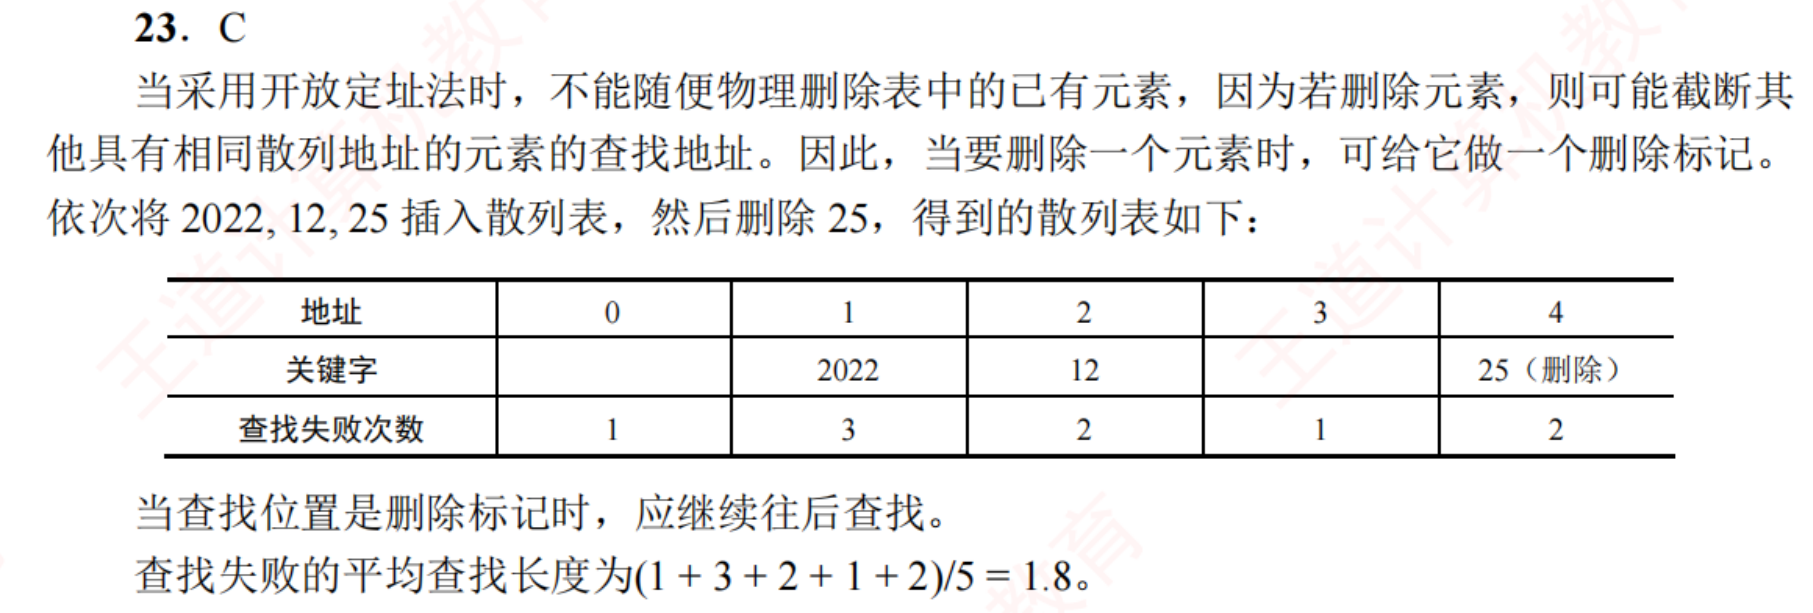
\includegraphics[width=161.13mm,height=180mm,keepaspectratio]{../solutions/assets/509e7ed5425214a362c39d59.png}\par\smallskip
\par\medskip\Needspace{5\baselineskip}\noindent\hypertarget{a:DS07-E08}{}\label{a:DS07-E08}\textbf{例 7-8}\quad HT={[}11,空,14,7,空,20,9,空,空,3,18{]}；7/11；3、18、14；地址7
\par\smallskip
20、3、11、18直接落5、9、0、10；9从5到6；14从9依次探测10、2；7从10依次探测0、3。最终0至10为\texttt{11,空,14,7,空,20,9,空,空,3,18}，装填因子\(7/11\)。查14访问9、10、2，比较3、18、14。查8初始地址2，按\(H_0+k^2\)探测2、3、6、0、7，在空地址7失败。

\section*{排序}
\par\medskip\Needspace{5\baselineskip}\noindent\hypertarget{a:DS08-E01}{}\label{a:DS08-E01}\textbf{例 8-1}\quad B
\par\smallskip
\par\medskip\noindent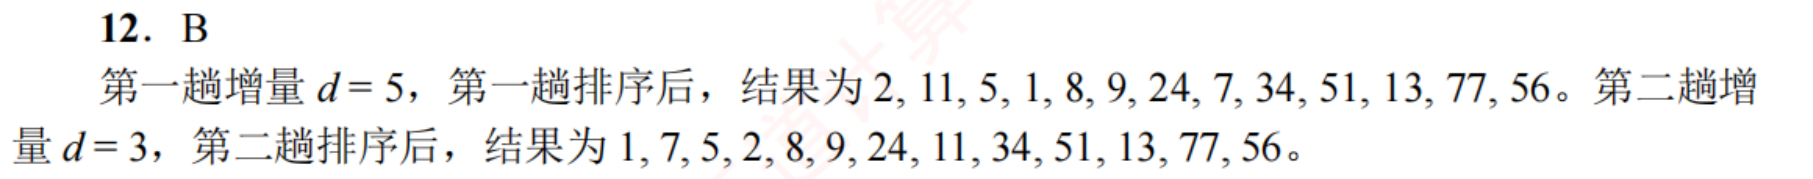
\includegraphics[width=161.13mm,height=180mm,keepaspectratio]{../solutions/assets/d05b70c4cae200bad1b783ae.png}\par\smallskip
\par\medskip\Needspace{5\baselineskip}\noindent\hypertarget{a:DS08-E02}{}\label{a:DS08-E02}\textbf{例 8-2}\quad D
\par\smallskip
\par\medskip\noindent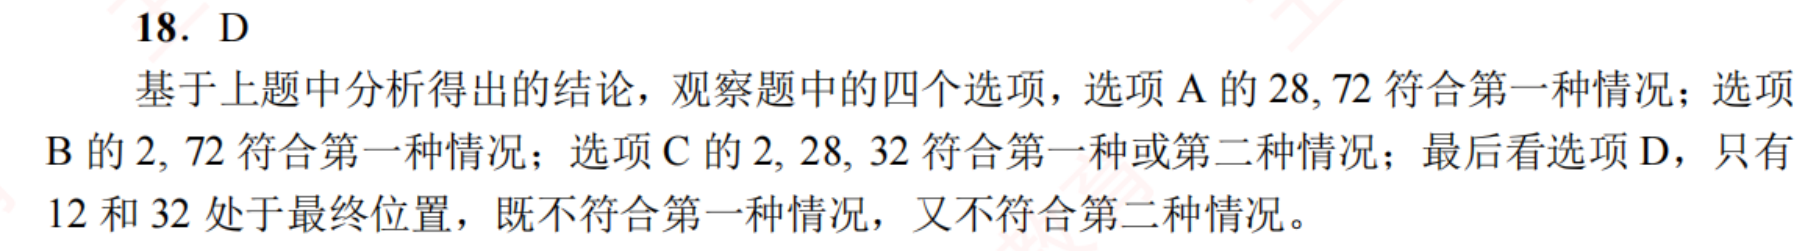
\includegraphics[width=161.13mm,height=180mm,keepaspectratio]{../solutions/assets/ca53037b04c718c96fb3bd9f.png}\par\smallskip
\par\medskip\Needspace{5\baselineskip}\noindent\hypertarget{a:DS08-E03}{}\label{a:DS08-E03}\textbf{例 8-3}\quad C
\par\smallskip
\par\medskip\noindent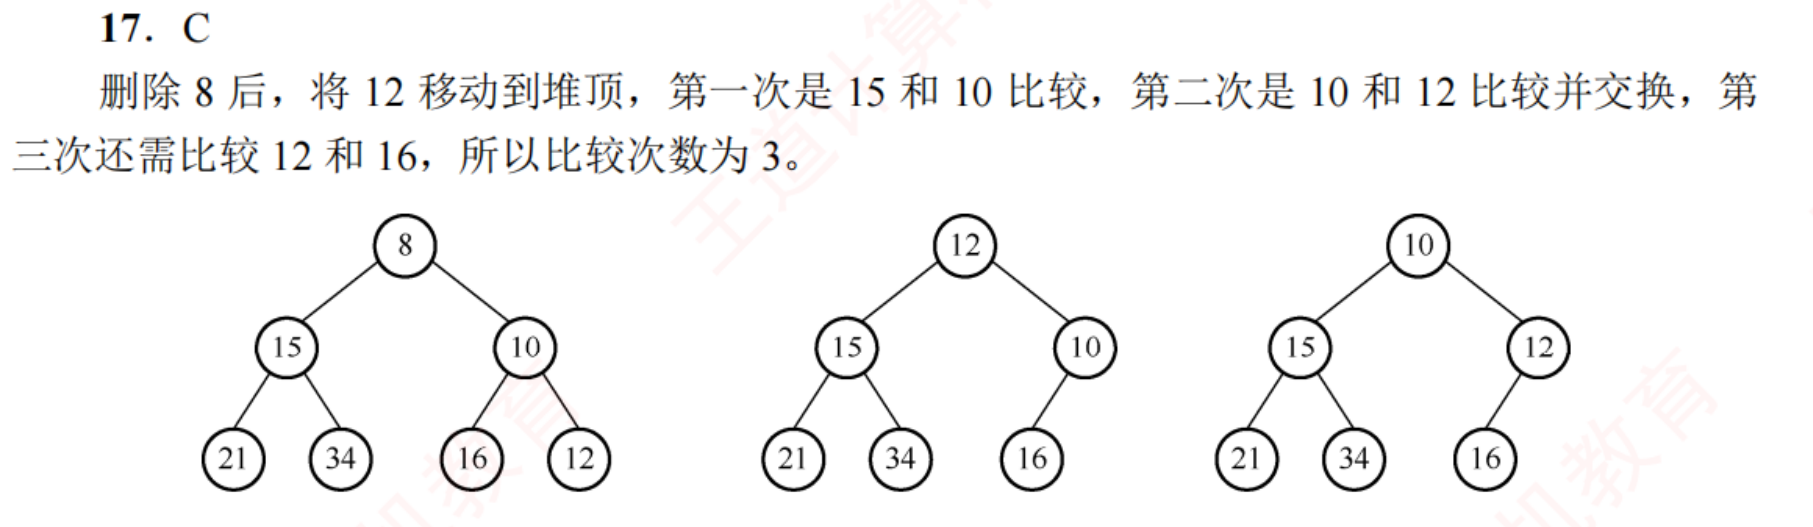
\includegraphics[width=161.13mm,height=180mm,keepaspectratio]{../solutions/assets/b90dd2a5bde6f698fd188c7e.png}\par\smallskip
\par\medskip\Needspace{5\baselineskip}\noindent\hypertarget{a:DS08-E04}{}\label{a:DS08-E04}\textbf{例 8-4}\quad C
\par\smallskip
\par\medskip\noindent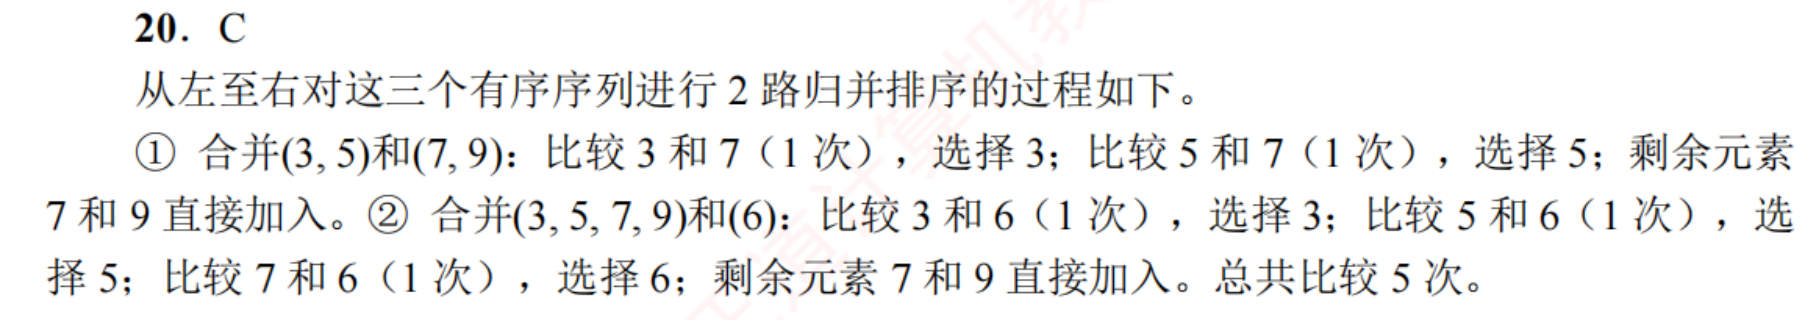
\includegraphics[width=161.13mm,height=180mm,keepaspectratio]{../solutions/assets/bdd205a1646697c5f4db4dd3.png}\par\smallskip
\par\medskip\Needspace{5\baselineskip}\noindent\hypertarget{a:DS08-E05}{}\label{a:DS08-E05}\textbf{例 8-5}\quad C
\par\smallskip
\par\medskip\noindent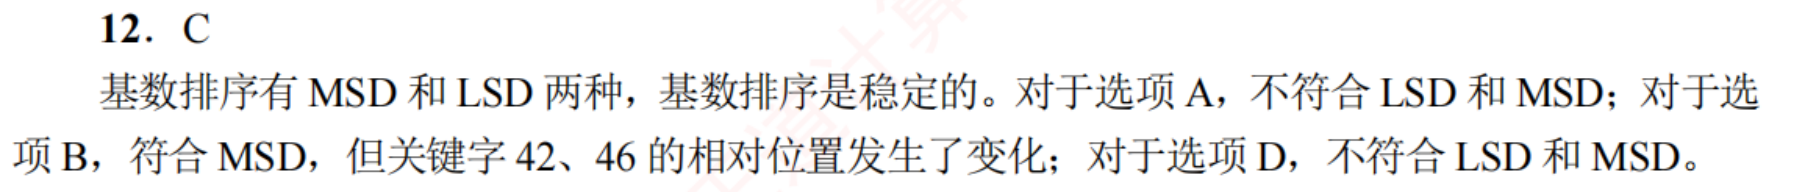
\includegraphics[width=161.13mm,height=180mm,keepaspectratio]{../solutions/assets/a660be9d17aee0019201ebaf.png}\par\smallskip
\par\medskip\Needspace{5\baselineskip}\noindent\hypertarget{a:DS08-E06}{}\label{a:DS08-E06}\textbf{例 8-6}\quad 3段；最大n，最小m
\par\smallskip
\par\medskip\noindent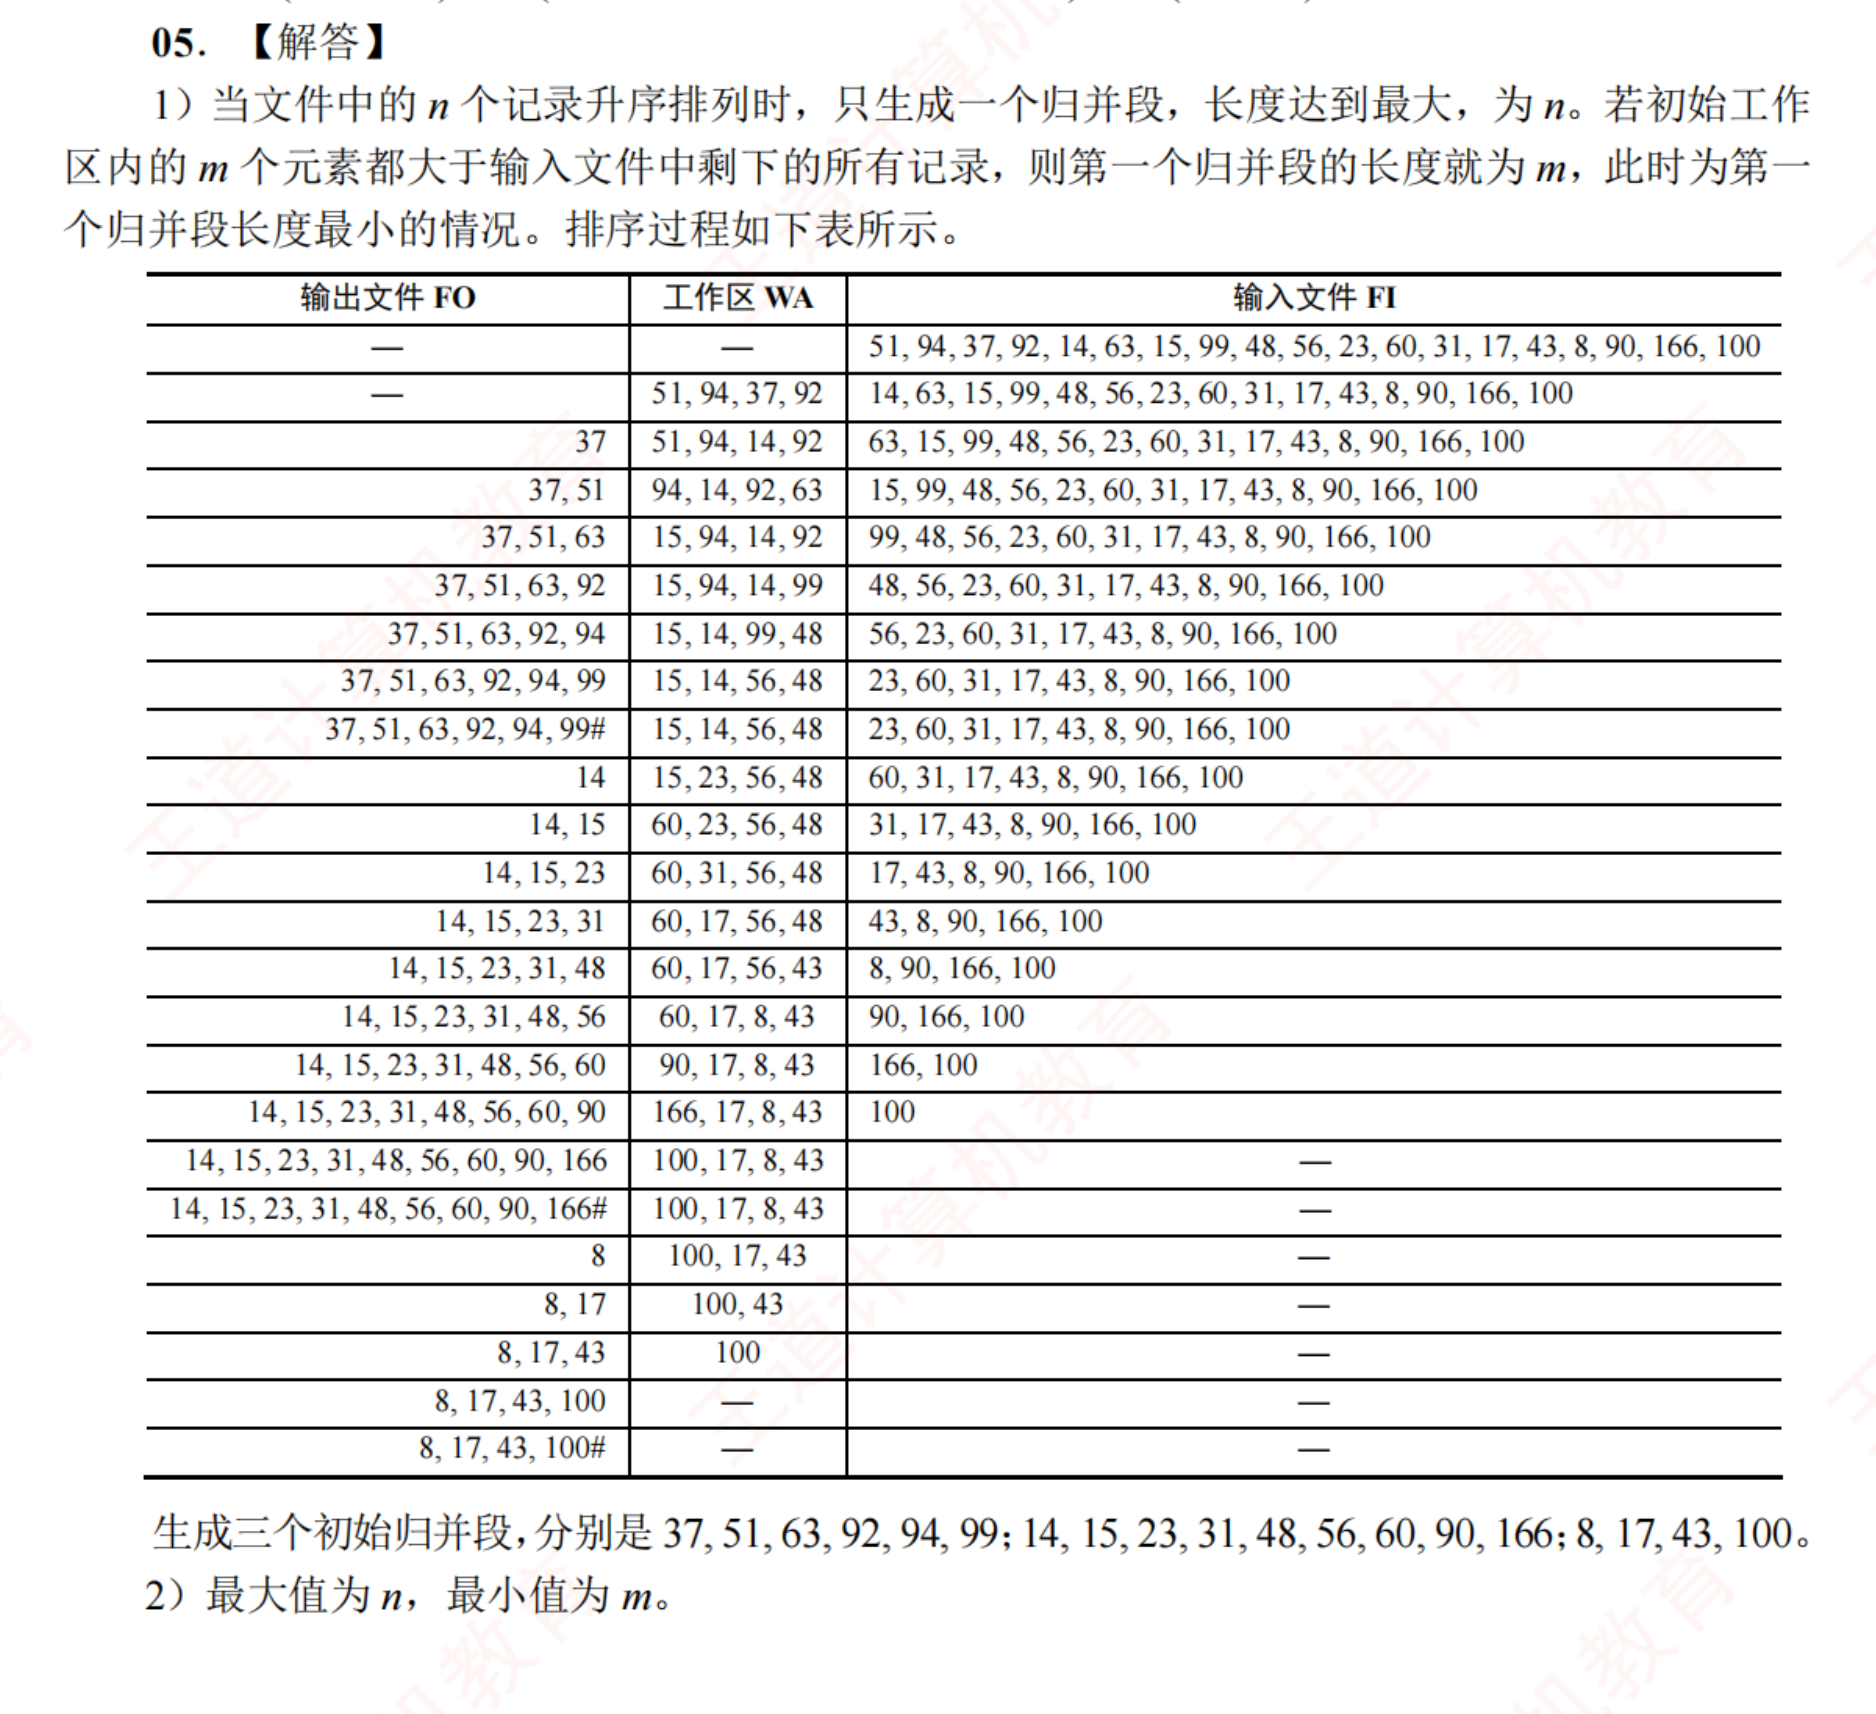
\includegraphics[width=162.00mm,height=180mm,keepaspectratio]{../solutions/assets/38d819fe7d2ab0be5ee67283.png}\par\smallskip
\par\medskip\Needspace{5\baselineskip}\noindent\hypertarget{a:DS08-E07}{}\label{a:DS08-E07}\textbf{例 8-7}\quad 825次；反复合并当前两个最短表
\par\smallskip
依次合并\texttt{10+35=45}、\texttt{40+45=85}、\texttt{50+60=110}、\texttt{85+110=195}、\texttt{195+200=395}。每次最坏比较数为新段长减1，合计\(44+84+109+194+394=825\)。合并长度和为WPL=830，减5次合并亦得825。对N表反复取最短两表，等价于以表长为叶权构造哈夫曼树，使重复参与层数的加权和最小。

\par\medskip\Needspace{5\baselineskip}\noindent\hypertarget{a:DS08-E08}{}\label{a:DS08-E08}\textbf{例 8-8}\quad WPL=690
\par\smallskip
\par\medskip\noindent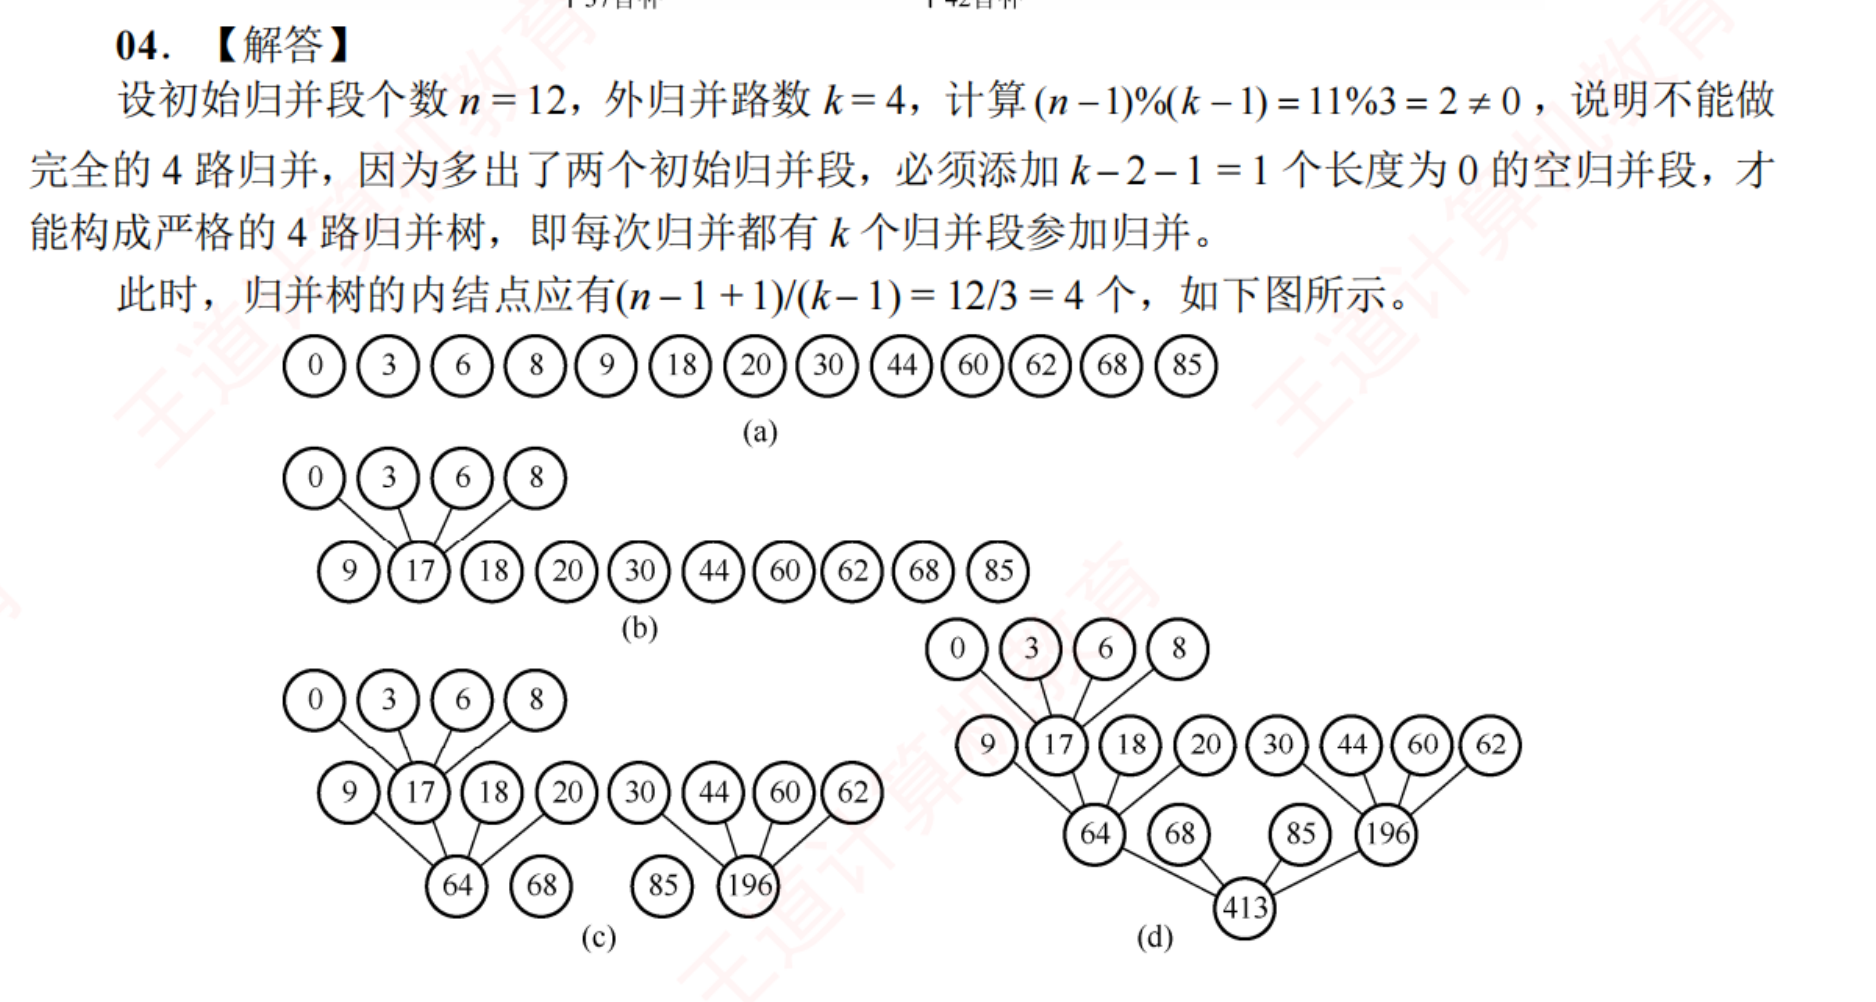
\includegraphics[width=162.00mm,height=180mm,keepaspectratio]{../solutions/assets/3a7b357a8db6154f8de1ec43.png}\par\smallskip
\par\medskip\noindent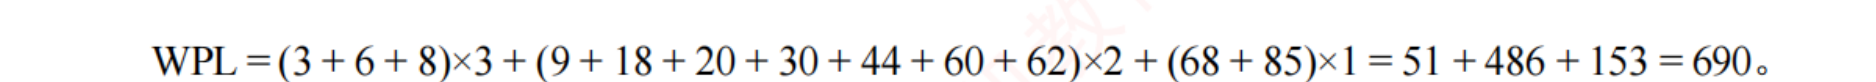
\includegraphics[width=162.00mm,height=180mm,keepaspectratio]{../solutions/assets/77bd9b46db503a2eaaecfd6d.png}\par\smallskip
\par\medskip\Needspace{5\baselineskip}\noindent\hypertarget{a:DS08-E09}{}\label{a:DS08-E09}\textbf{例 8-9}\quad 随机划分选择第10小，平均时间\(O(n)\)、迭代辅助空间\(O(1)\)
\par\smallskip
用随机枢轴划分，只继续处理包含第10小这一秩的子区间，丢弃无需继续划分的一侧。确定分界后保留10个最小数，无须内部有序；相等值跨边界时按尚需个数取足。随机选择的期望工作量为\(O(n)\)，在原数组迭代执行辅助空间\(O(1)\)。也可用大小10的大根堆扫描，只有新值小于堆顶才替换、下滤，时间\(O(n\log10)\)、辅助空间\(O(10)\)，适合流式输入。

\chapter{计算机组成原理}
\section*{计算机系统与程序执行的层次}
\par\medskip\Needspace{5\baselineskip}\noindent\hypertarget{a:CO01-E01}{}\label{a:CO01-E01}\textbf{例 1-1}\quad A
\par\smallskip
\par\medskip\noindent
\includegraphics[width=161.13mm,height=180mm,keepaspectratio]{../solutions/assets/fd5fb050448a47b15f59949a.png}\par\smallskip
\par\medskip\Needspace{5\baselineskip}\noindent\hypertarget{a:CO01-E02}{}\label{a:CO01-E02}\textbf{例 1-2}\quad A，平均 CPI=2.8，CPU 时间28 μs。
\par\smallskip
\par\medskip\noindent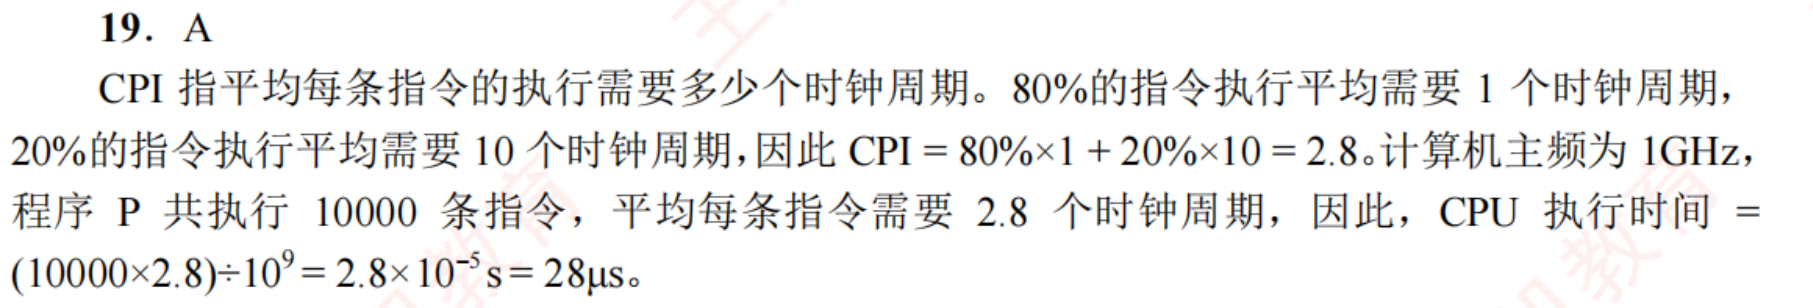
\includegraphics[width=161.13mm,height=180mm,keepaspectratio]{../solutions/assets/9ff14a554d61fbe541f77ad1.png}\par\smallskip
\par\medskip\Needspace{5\baselineskip}\noindent\hypertarget{a:CO01-E03}{}\label{a:CO01-E03}\textbf{例 1-3}\quad D，70 s。
\par\smallskip
\par\medskip\noindent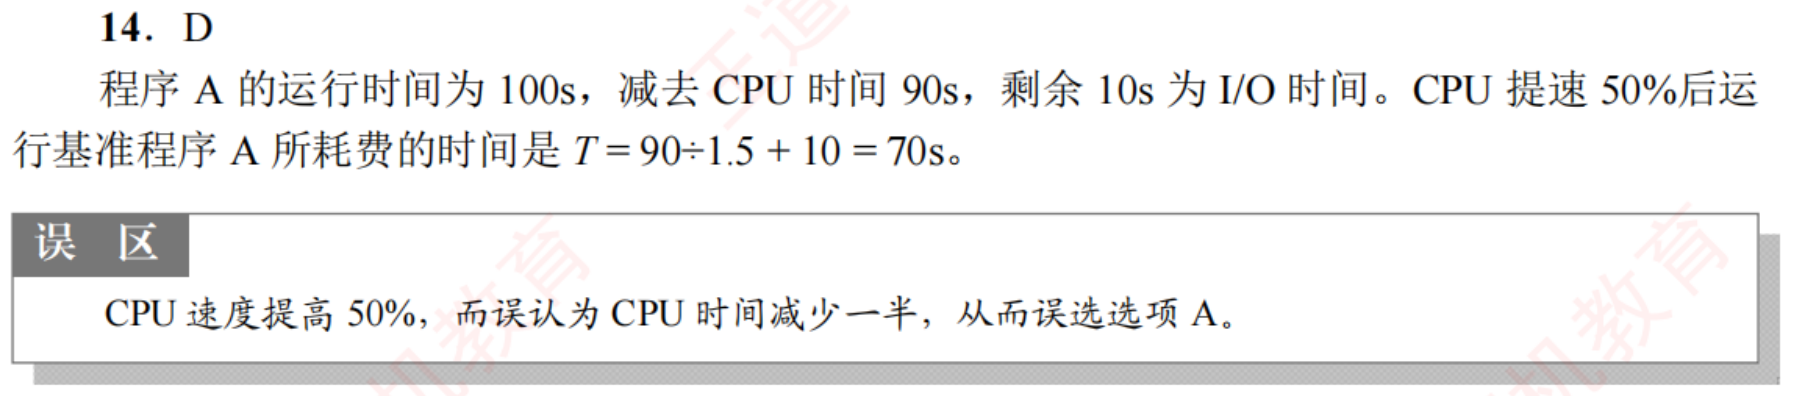
\includegraphics[width=161.13mm,height=180mm,keepaspectratio]{../solutions/assets/0ed1923bf20cdfc73f529985.png}\par\smallskip
\section*{数据表示、位级运算与浮点数}
\par\medskip\Needspace{5\baselineskip}\noindent\hypertarget{a:CO02-E01}{}\label{a:CO02-E01}\textbf{例 2-1}\quad B，211.4。
\par\smallskip
\par\medskip\noindent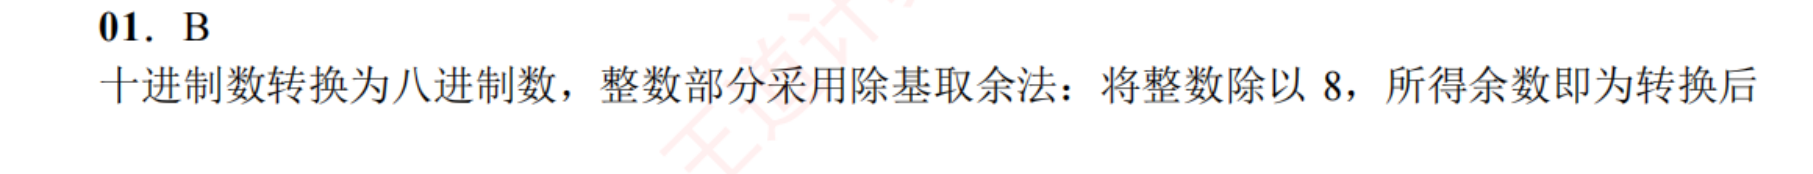
\includegraphics[width=161.13mm,height=180mm,keepaspectratio]{../solutions/assets/5fbe3a0987c2ec914058d0b8.png}\par\smallskip
\par\medskip\noindent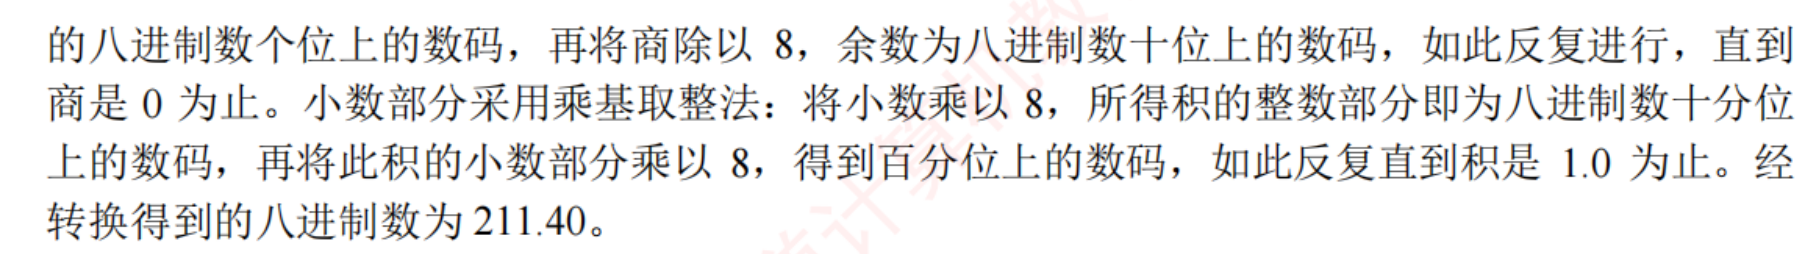
\includegraphics[width=161.13mm,height=180mm,keepaspectratio]{../solutions/assets/c20d63b9123adf0db02765ce.png}\par\smallskip
\par\medskip\Needspace{5\baselineskip}\noindent\hypertarget{a:CO02-E02}{}\label{a:CO02-E02}\textbf{例 2-2}\quad B，0000 FFFAH。
\par\smallskip
\par\medskip\noindent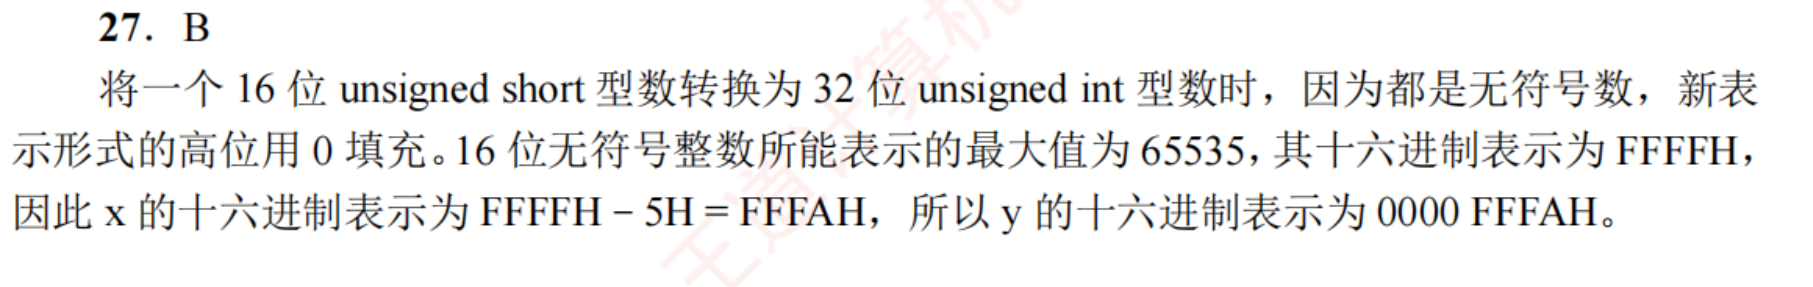
\includegraphics[width=161.13mm,height=180mm,keepaspectratio]{../solutions/assets/9acfee66561648f8d23e672b.png}\par\smallskip
\par\medskip\noindent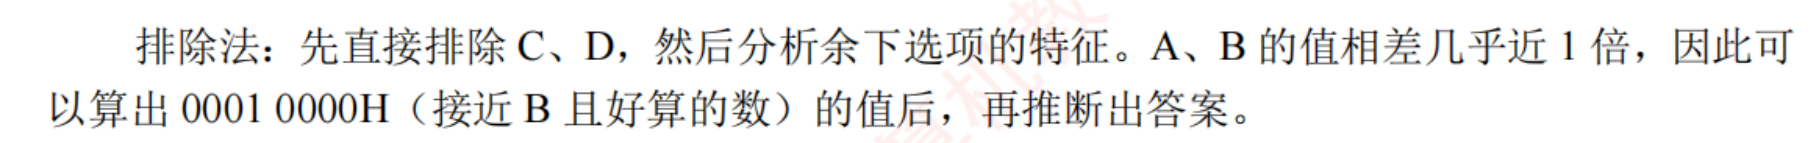
\includegraphics[width=161.13mm,height=180mm,keepaspectratio]{../solutions/assets/2bc518e48d9d2fdc93992225.png}\par\smallskip
\par\medskip\Needspace{5\baselineskip}\noindent\hypertarget{a:CO02-E03}{}\label{a:CO02-E03}\textbf{例 2-3}\quad D。
\par\smallskip
\par\medskip\noindent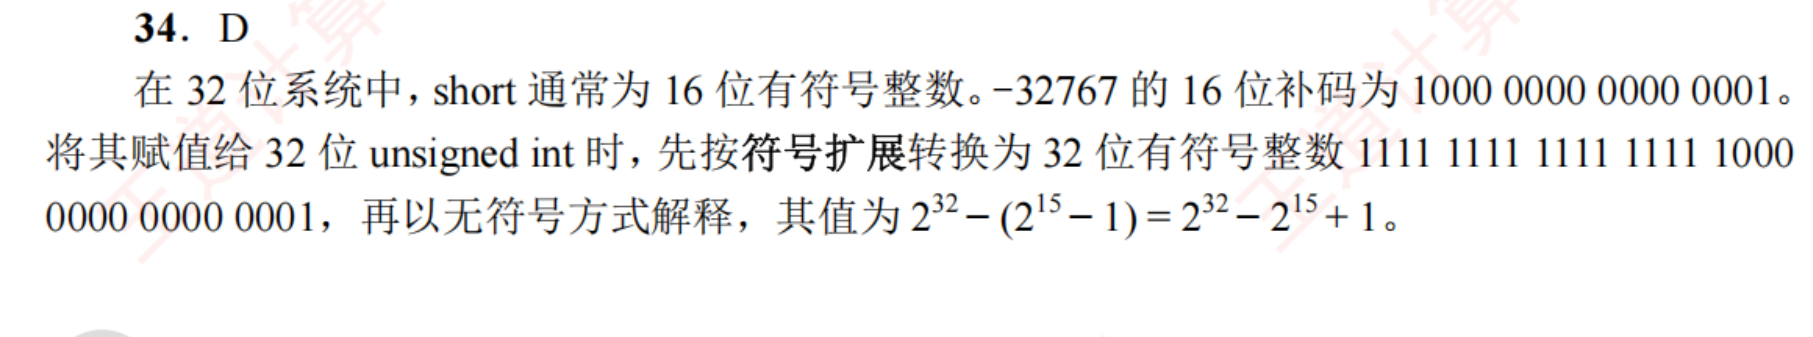
\includegraphics[width=161.13mm,height=180mm,keepaspectratio]{../solutions/assets/e659abc4867b17dbb350fd38.png}\par\smallskip
\par\medskip\Needspace{5\baselineskip}\noindent\hypertarget{a:CO02-E04}{}\label{a:CO02-E04}\textbf{例 2-4}\quad B。
\par\smallskip
\par\medskip\noindent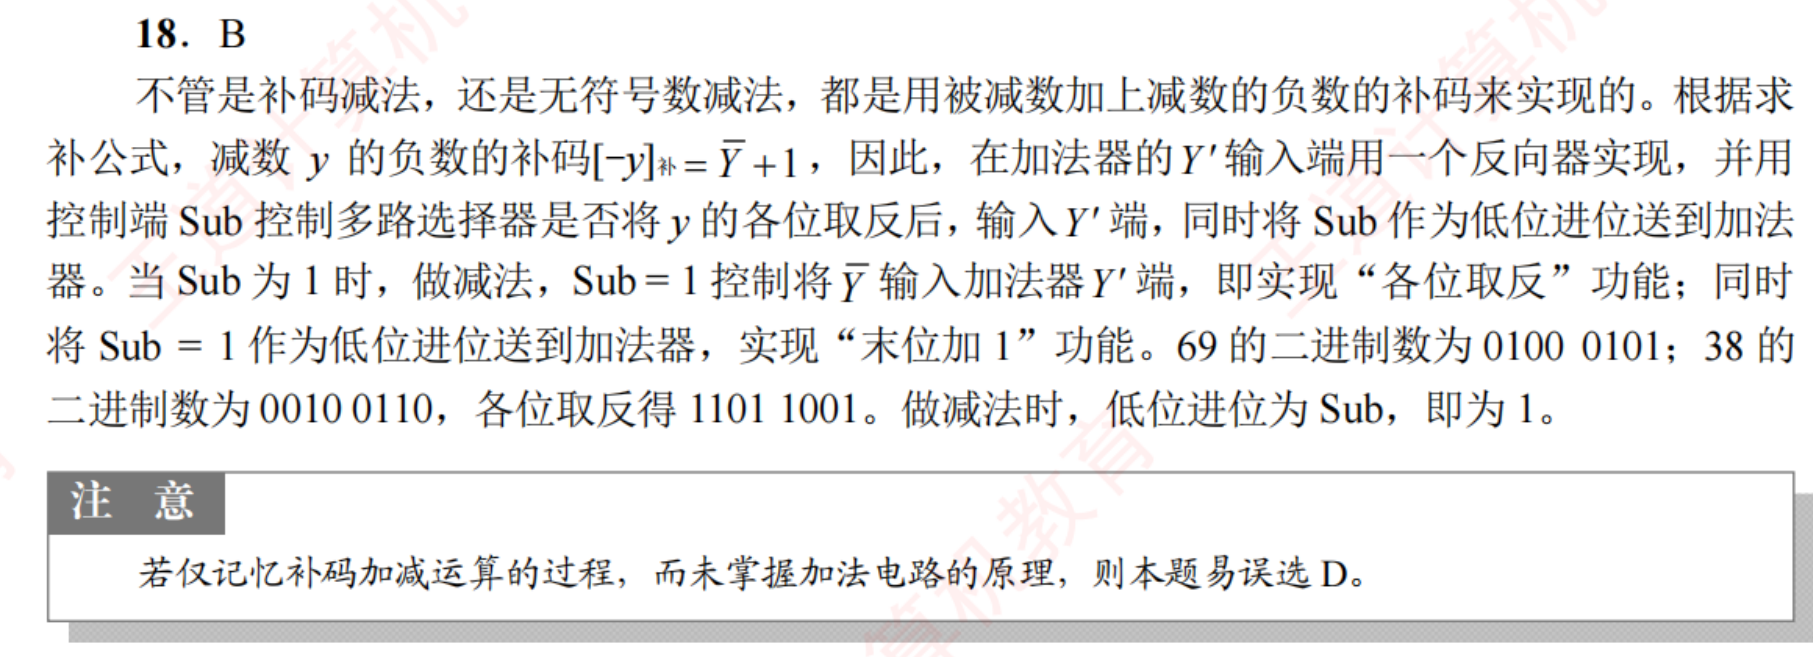
\includegraphics[width=161.13mm,height=180mm,keepaspectratio]{../solutions/assets/d7fa9c92d1ab1763341a6a5d.png}\par\smallskip
\par\medskip\Needspace{5\baselineskip}\noindent\hypertarget{a:CO02-E05}{}\label{a:CO02-E05}\textbf{例 2-5}\quad C。
\par\smallskip
\par\medskip\noindent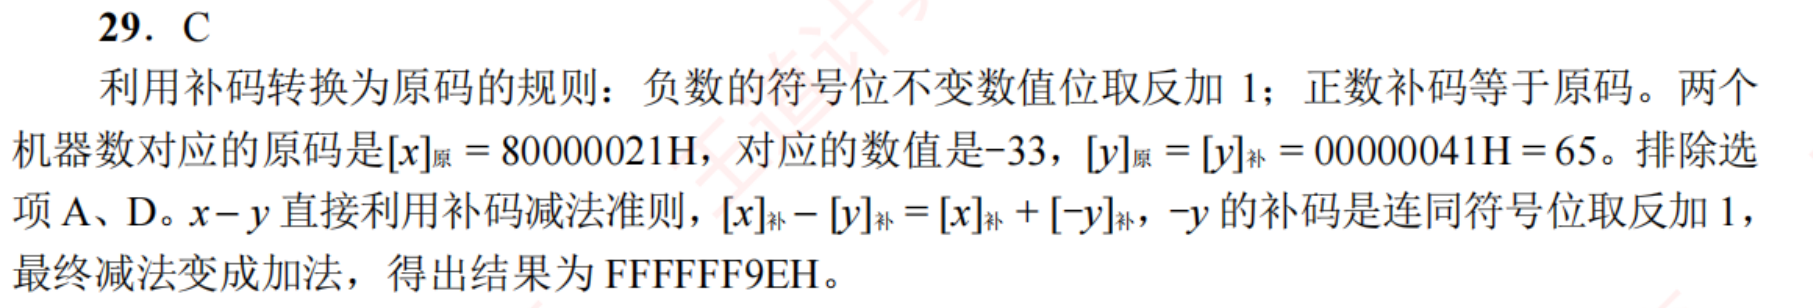
\includegraphics[width=161.13mm,height=180mm,keepaspectratio]{../solutions/assets/ce841085c325d5dcdb9cce63.png}\par\smallskip
\par\medskip\Needspace{5\baselineskip}\noindent\hypertarget{a:CO02-E06}{}\label{a:CO02-E06}\textbf{例 2-6}\quad B，OF=0、CF=1。
\par\smallskip
\par\medskip\noindent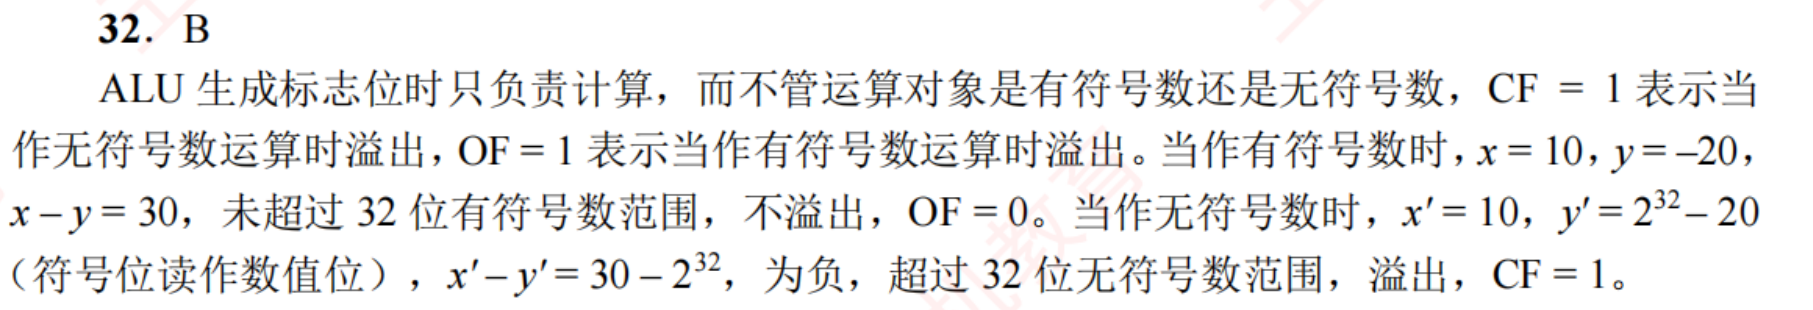
\includegraphics[width=161.13mm,height=180mm,keepaspectratio]{../solutions/assets/f7d57aa03f5716d0c6e453e2.png}\par\smallskip
\par\medskip\Needspace{5\baselineskip}\noindent\hypertarget{a:CO02-E07}{}\label{a:CO02-E07}\textbf{例 2-7}\quad A，BEE0 0000H。
\par\smallskip
\par\medskip\noindent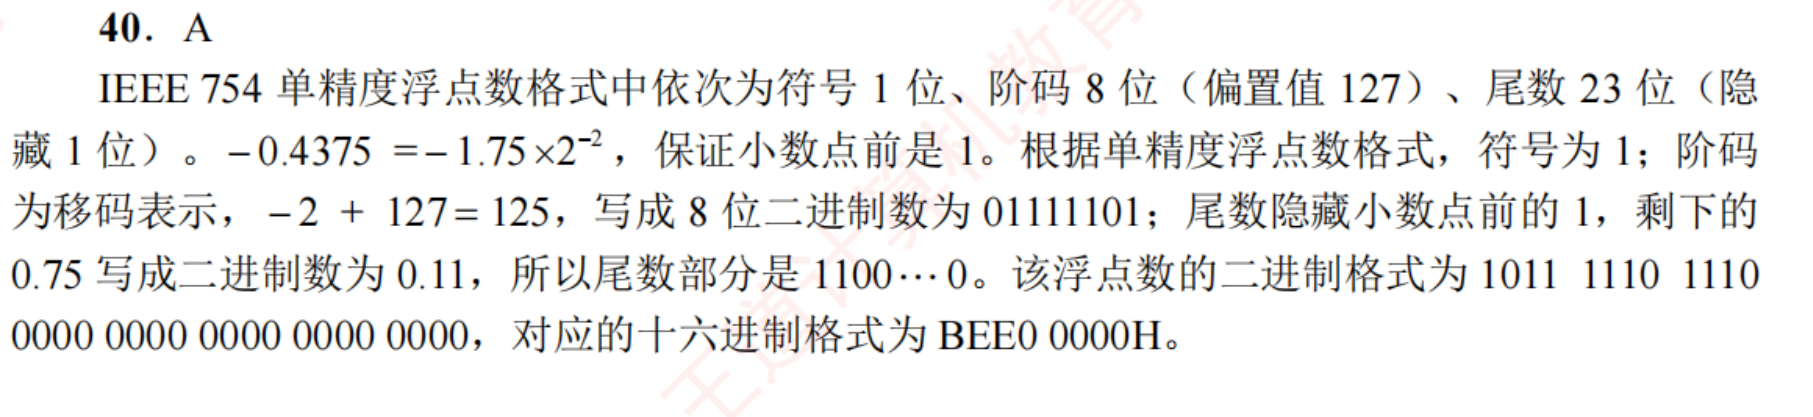
\includegraphics[width=161.13mm,height=180mm,keepaspectratio]{../solutions/assets/056beccb851b7d12795ca177.png}\par\smallskip
\par\medskip\noindent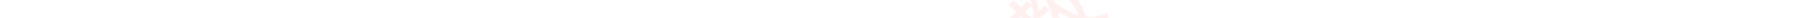
\includegraphics[width=161.13mm,height=180mm,keepaspectratio]{../solutions/assets/97794e24782089ccaed3abb8.png}\par\smallskip
\par\medskip\Needspace{5\baselineskip}\noindent\hypertarget{a:CO02-E08}{}\label{a:CO02-E08}\textbf{例 2-8}\quad A，x\textless y且符号相同。
\par\smallskip
\par\medskip\noindent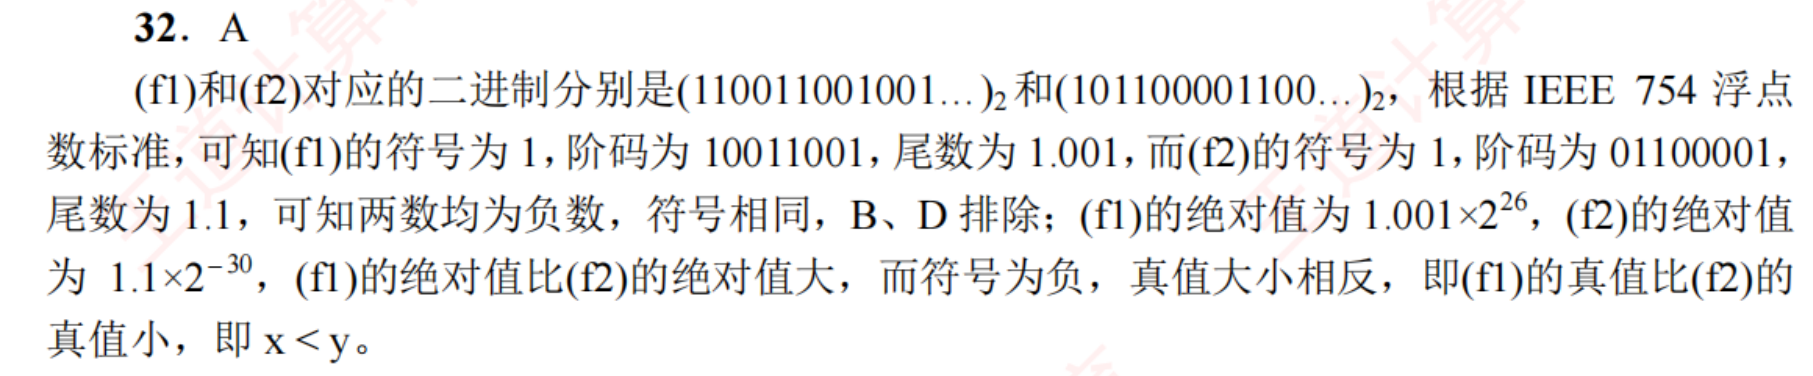
\includegraphics[width=161.13mm,height=180mm,keepaspectratio]{../solutions/assets/f329c7f0590d4e71f00e20e2.png}\par\smallskip
\par\medskip\Needspace{5\baselineskip}\noindent\hypertarget{a:CO02-E09}{}\label{a:CO02-E09}\textbf{例 2-9}\quad D，I、II、III、IV。
\par\smallskip
\par\medskip\noindent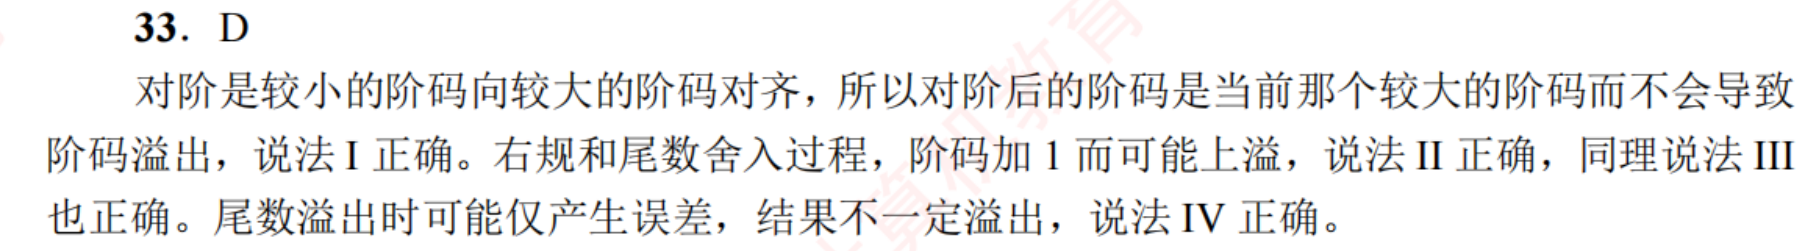
\includegraphics[width=161.13mm,height=180mm,keepaspectratio]{../solutions/assets/bc28bf433c8ea18cfbe551b6.png}\par\smallskip
\par\medskip\Needspace{5\baselineskip}\noindent\hypertarget{a:CO02-E10}{}\label{a:CO02-E10}\textbf{例 2-10}\quad （1）机器模型下循环条件恒真；改int后不进入循环。（2）相等；00FF FFFFH、4B7F FFFFH。（3）浮点舍入为2\^{}25。（4）低32位全1；最大n=30。（5）正无穷；不溢出最大n=126，精确最大n=23。
\par\smallskip
本题关于f1溢出后的返回值、n=0的持续循环按题设32位补码机器模型推演；C有符号溢出属未定义行为。

（1）unsigned的 \texttt{n-1} 在n=0时为 \(2^{32}-1\)，任意unsigned i均满足条件，i递增可绕回0。若i、n改int，首次条件为 \(0\le-1\)，循环不执行。

（2）\(f(23)=2^{24}-1=16777215\)，int和24位精度binary32均精确。int机器数00FF FFFFH；浮点 \(1.\underbrace{11\cdots1}_{23\text{位}}\times2^{23}\)，阶码150，机器数4B7F FFFFH。

（3）\(f(24)=2^{25}-1=33554431\) 需25位精度；binary32相邻候选为33554430、33554432，精确和居中，最近偶数取33554432，即4C00 0000H。

（4）\(2^{32}-1\) 超过int上界，机器模型保留低32位全1，补码为\ensuremath{-}1。精确须 \(2^{n+1}-1\le2^{31}-1\)，故n\ensuremath{\le}30。

（5）7F80 0000H表示正无穷。n=126的结果舍入为有限 \(2^{127}\)；n=127越过有限上界并舍入为无穷。不溢出上界126；完全精确需n+1个连续1全部容纳在24位中，上界23。

\par\medskip\Needspace{5\baselineskip}\noindent\hypertarget{a:CO02-E11}{}\label{a:CO02-E11}\textbf{例 2-11}\quad D，0x11、0xC00E。
\par\smallskip
\par\medskip\noindent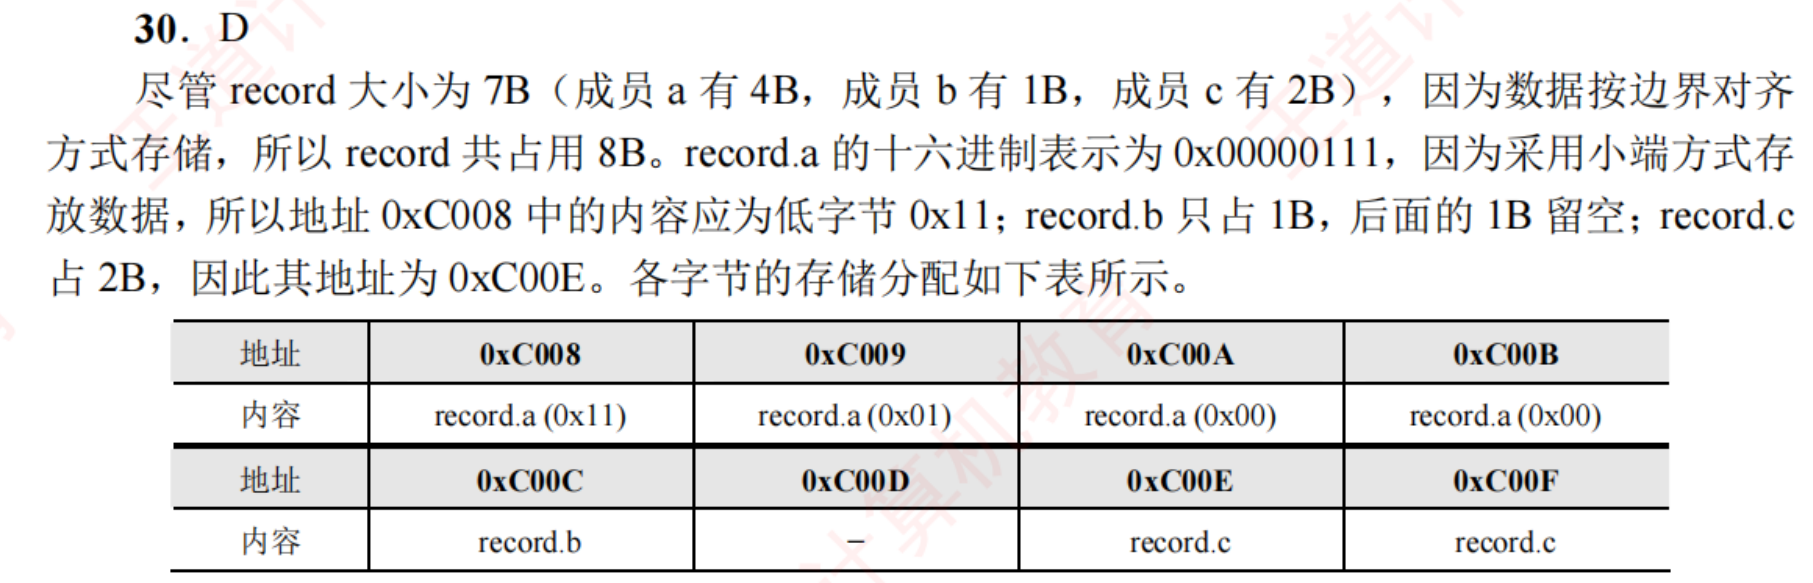
\includegraphics[width=161.13mm,height=180mm,keepaspectratio]{../solutions/assets/f9b052e6bd3bee25987f64f4.png}\par\smallskip
\section*{存储层次、地址与 Cache}
\par\medskip\Needspace{5\baselineskip}\noindent\hypertarget{a:CO03-E01}{}\label{a:CO03-E01}\textbf{例 3-1}\quad A，19根。
\par\smallskip
\par\medskip\noindent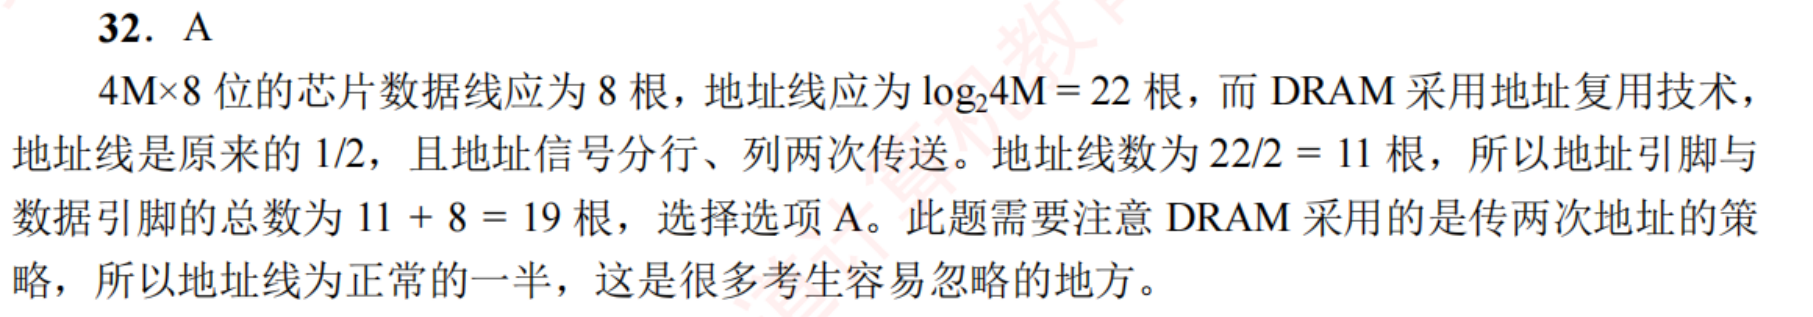
\includegraphics[width=161.13mm,height=180mm,keepaspectratio]{../solutions/assets/d98ed26634a5d3bd08500f44.png}\par\smallskip
\par\medskip\Needspace{5\baselineskip}\noindent\hypertarget{a:CO03-E02}{}\label{a:CO03-E02}\textbf{例 3-2}\quad D，26位。
\par\smallskip
\par\medskip\noindent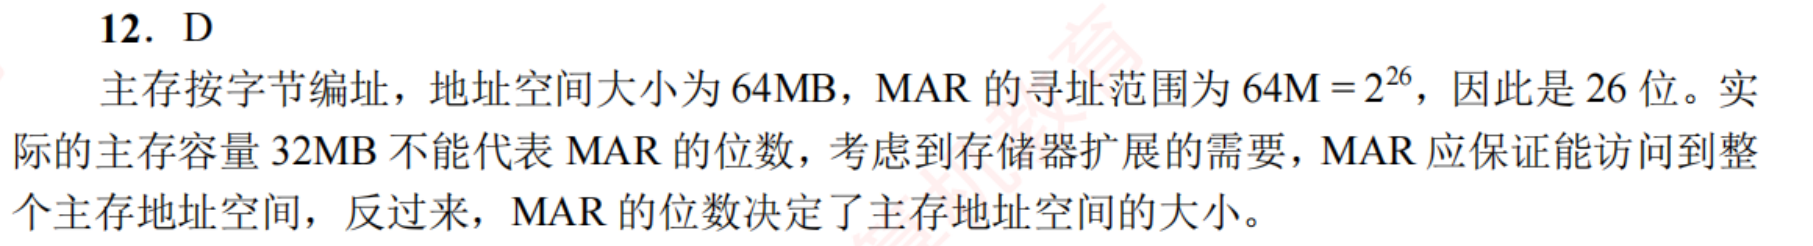
\includegraphics[width=161.13mm,height=180mm,keepaspectratio]{../solutions/assets/0dc914bc82d69a73df1133ab.png}\par\smallskip
\par\medskip\Needspace{5\baselineskip}\noindent\hypertarget{a:CO03-E03}{}\label{a:CO03-E03}\textbf{例 3-3}\quad D，8000和8004。
\par\smallskip
\par\medskip\noindent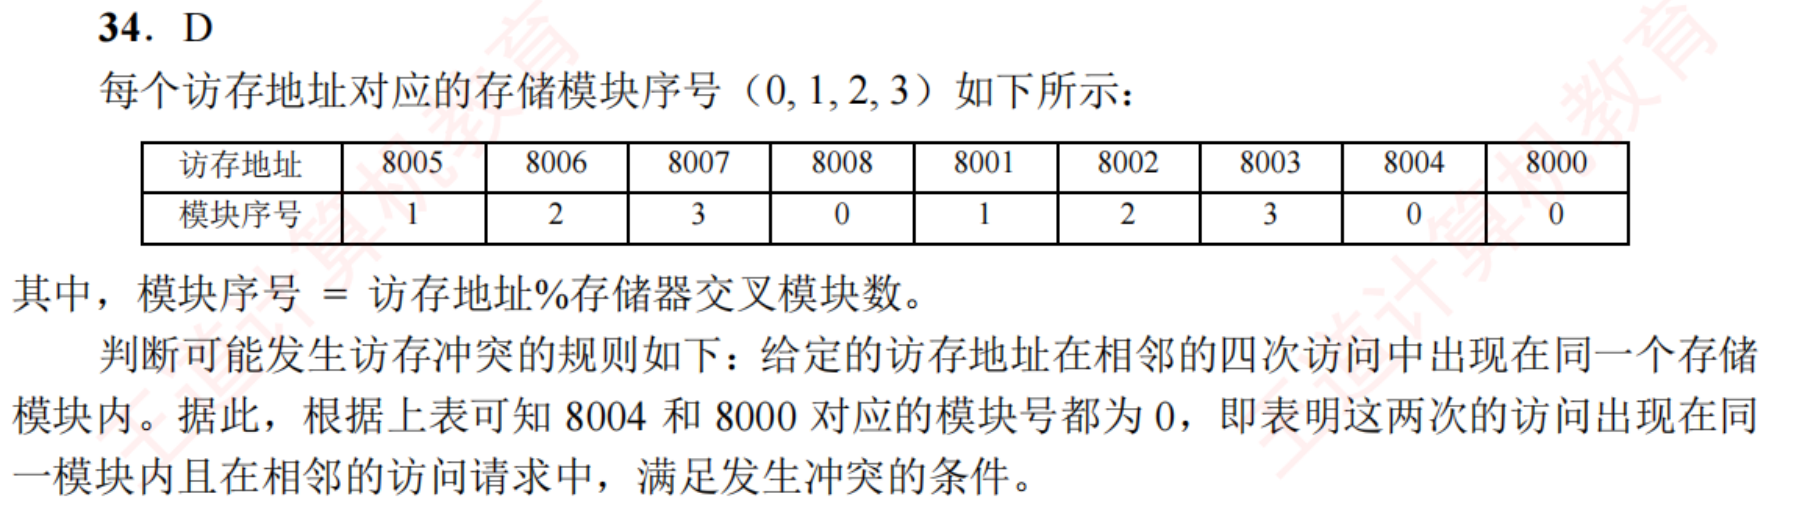
\includegraphics[width=161.13mm,height=180mm,keepaspectratio]{../solutions/assets/c134a0bc53edb41ad0b398d8.png}\par\smallskip
\par\medskip\Needspace{5\baselineskip}\noindent\hypertarget{a:CO03-E04}{}\label{a:CO03-E04}\textbf{例 3-4}\quad D，ROM 2片、RAM 30片。
\par\smallskip
\par\medskip\noindent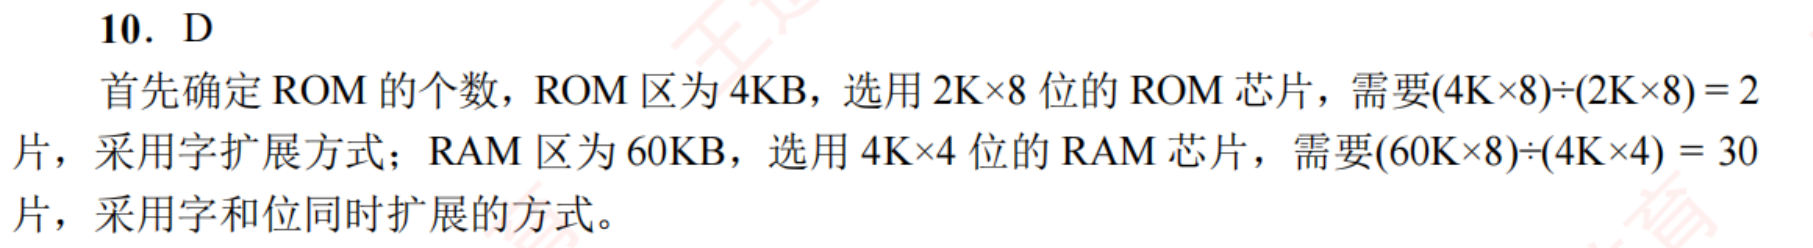
\includegraphics[width=161.13mm,height=180mm,keepaspectratio]{../solutions/assets/265307aaaa7088857604c964.png}\par\smallskip
\par\medskip\Needspace{5\baselineskip}\noindent\hypertarget{a:CO03-E05}{}\label{a:CO03-E05}\textbf{例 3-5}\quad B，约12.2 ms。
\par\smallskip
\par\medskip\noindent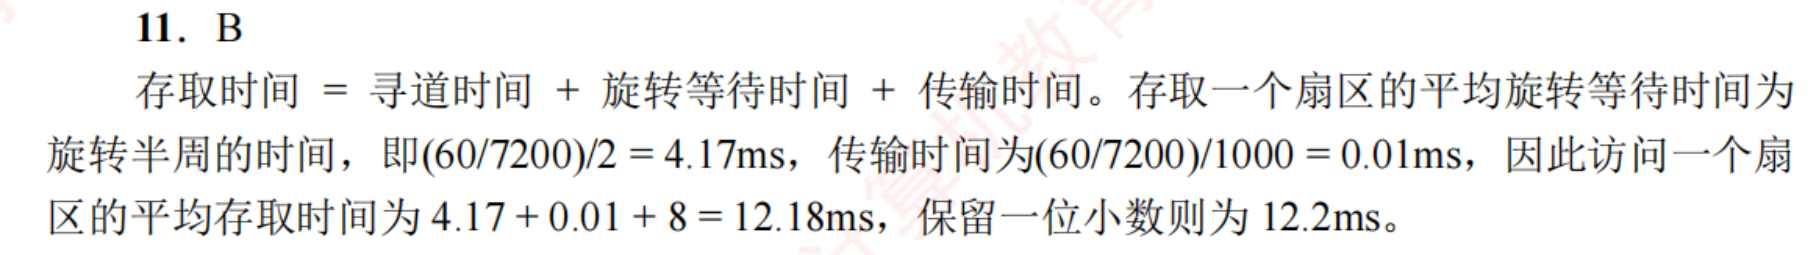
\includegraphics[width=161.13mm,height=180mm,keepaspectratio]{../solutions/assets/d8a5bf80b54727a38ab07d4d.png}\par\smallskip
\par\medskip\Needspace{5\baselineskip}\noindent\hypertarget{a:CO03-E06}{}\label{a:CO03-E06}\textbf{例 3-6}\quad C，约12.5\%。
\par\smallskip
\par\medskip\noindent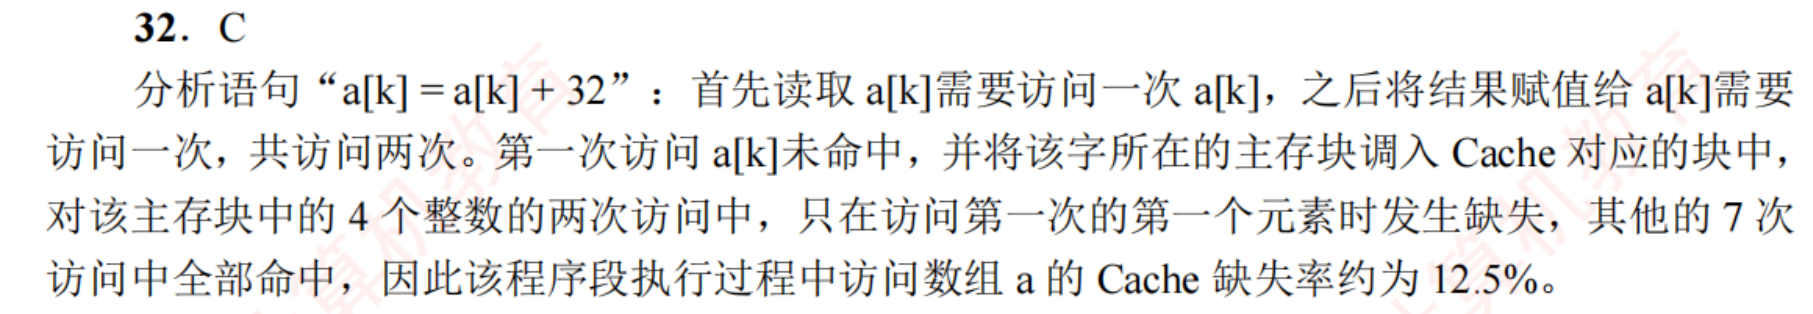
\includegraphics[width=161.13mm,height=180mm,keepaspectratio]{../solutions/assets/79e811d2b5fc25d803e255c6.png}\par\smallskip
\par\medskip\Needspace{5\baselineskip}\noindent\hypertarget{a:CO03-E07}{}\label{a:CO03-E07}\textbf{例 3-7}\quad A，8个20位比较器。
\par\smallskip
\par\medskip\noindent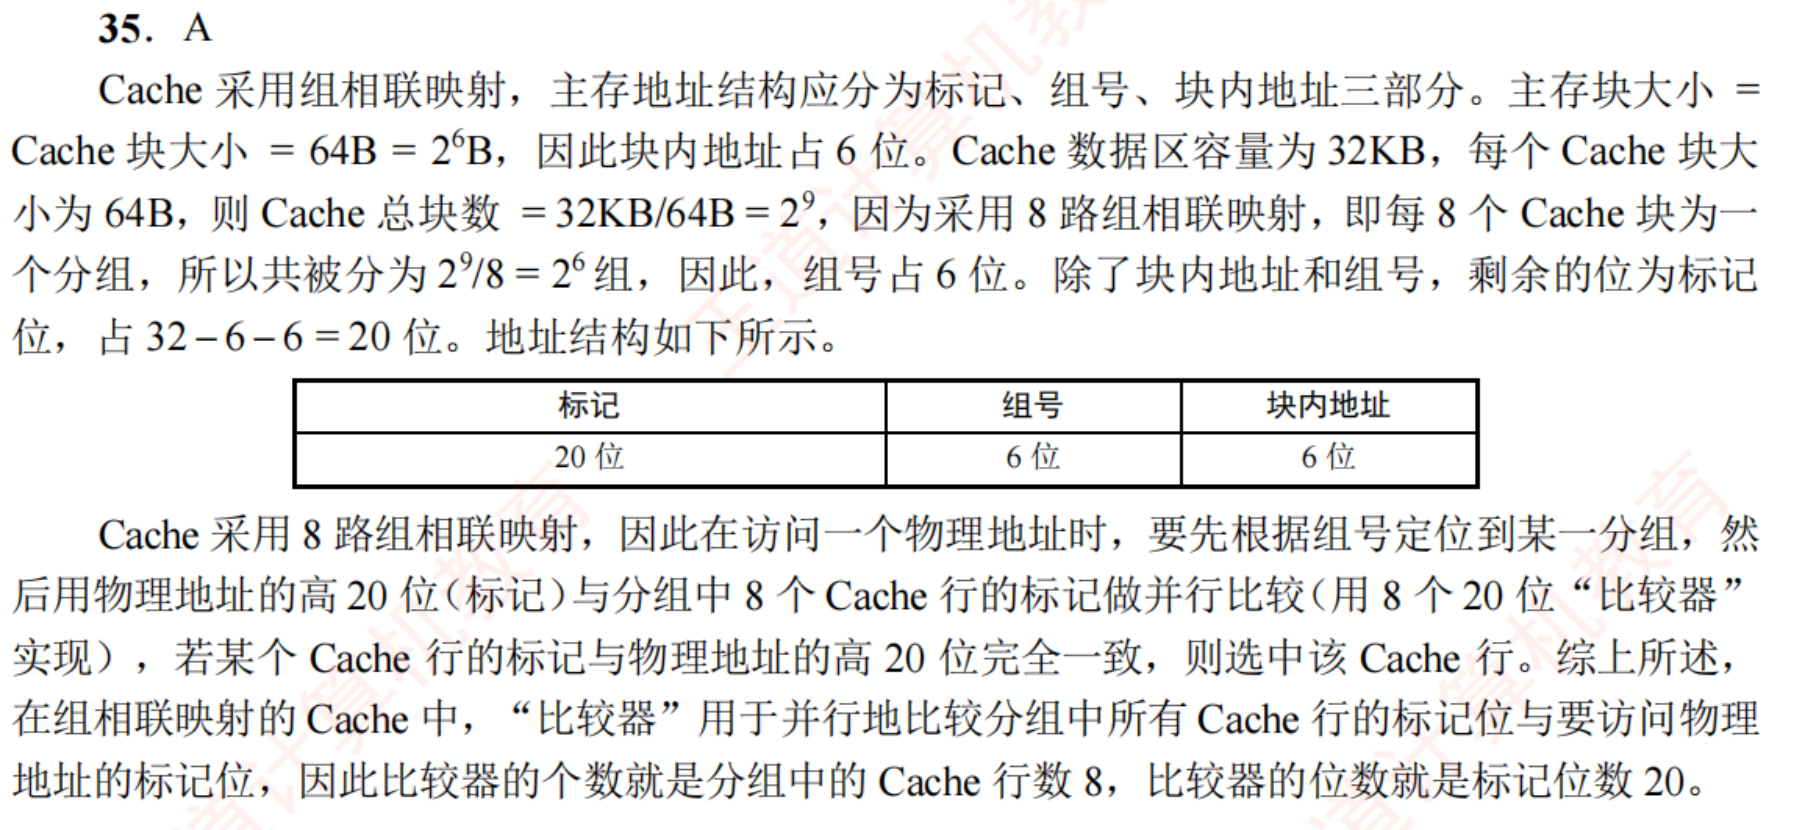
\includegraphics[width=161.13mm,height=180mm,keepaspectratio]{../solutions/assets/cfd24cfe5dc380deaa9be0ab.png}\par\smallskip
\par\medskip\Needspace{5\baselineskip}\noindent\hypertarget{a:CO03-E08}{}\label{a:CO03-E08}\textbf{例 3-8}\quad C，148 K位。
\par\smallskip
\par\medskip\noindent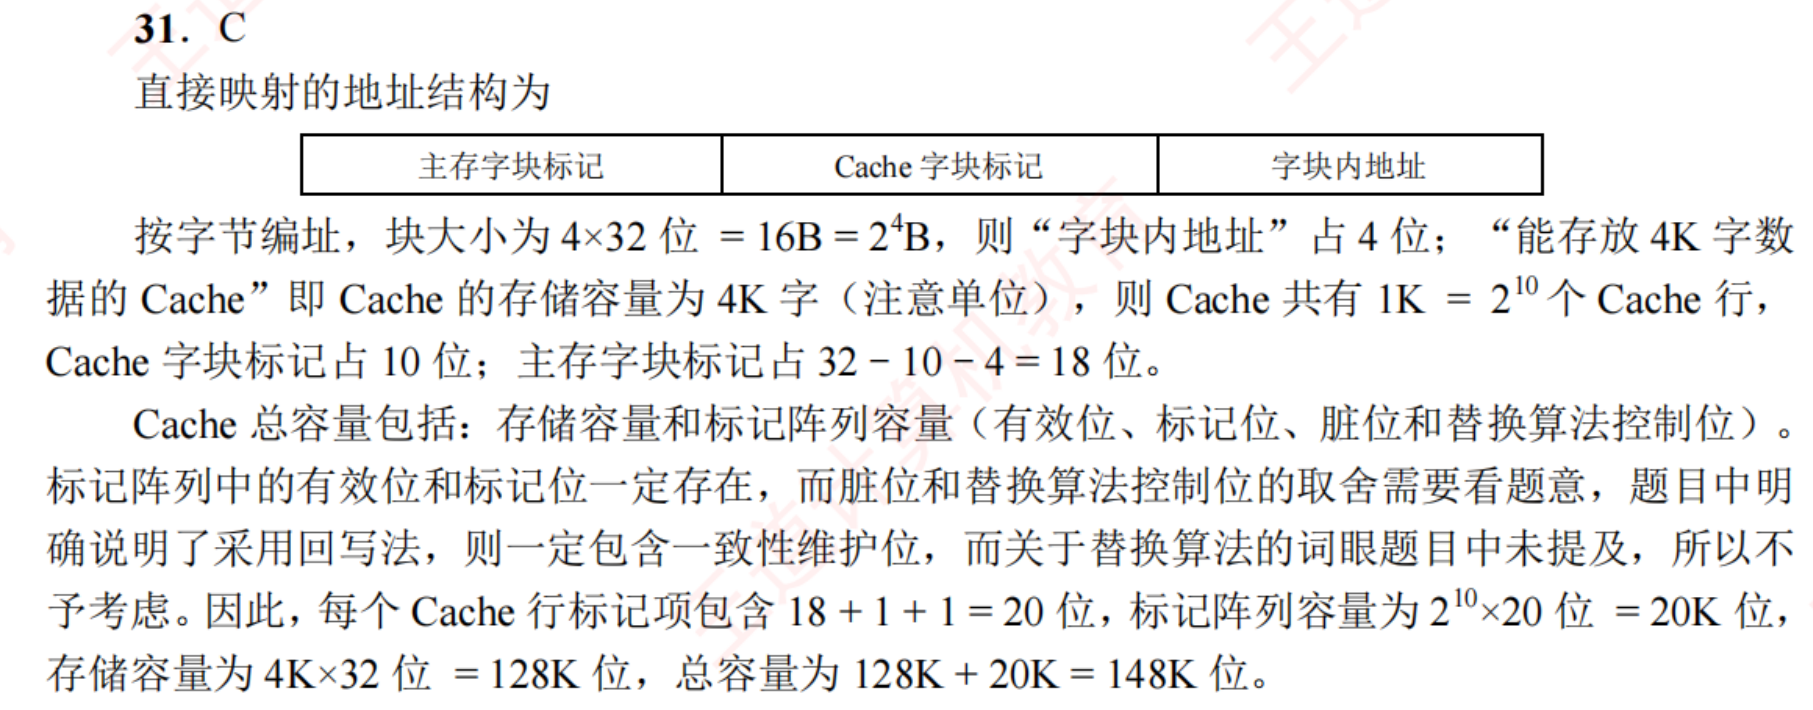
\includegraphics[width=161.13mm,height=180mm,keepaspectratio]{../solutions/assets/23ec5a975278601b25c90f05.png}\par\smallskip
\par\medskip\Needspace{5\baselineskip}\noindent\hypertarget{a:CO03-E09}{}\label{a:CO03-E09}\textbf{例 3-9}\quad C，01 8840H。
\par\smallskip
\par\medskip\noindent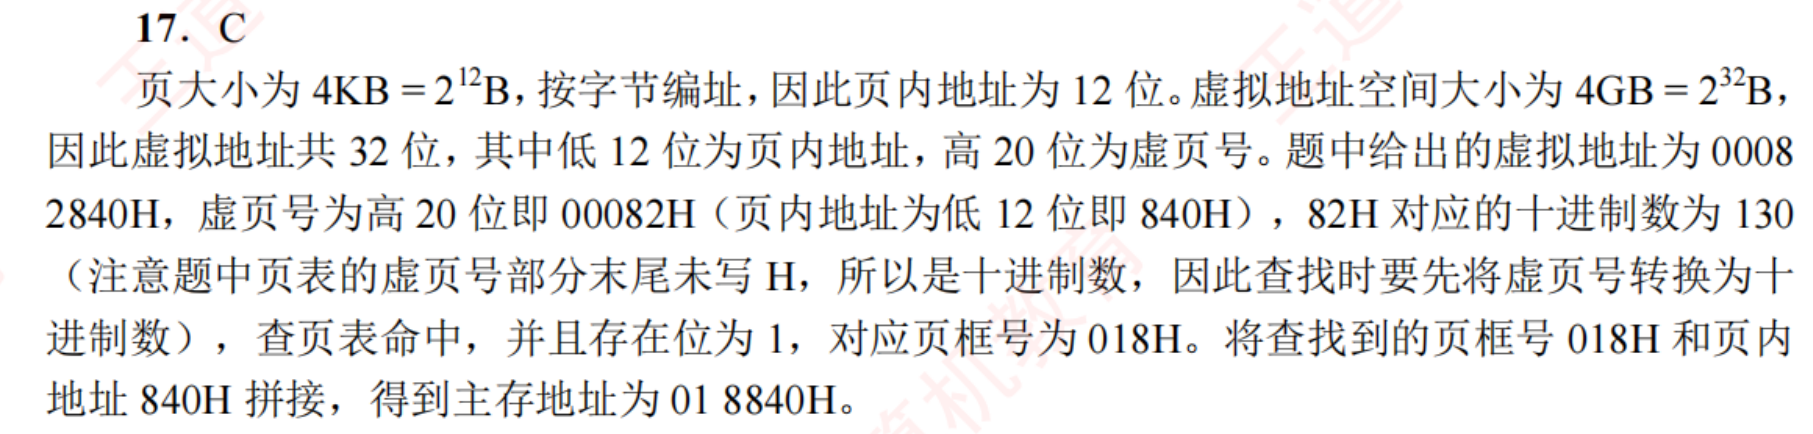
\includegraphics[width=161.13mm,height=180mm,keepaspectratio]{../solutions/assets/b9c68c41f01623e4def997a9.png}\par\smallskip
\par\medskip\Needspace{5\baselineskip}\noindent\hypertarget{a:CO03-E10}{}\label{a:CO03-E10}\textbf{例 3-10}\quad C，19位。
\par\smallskip
\par\medskip\noindent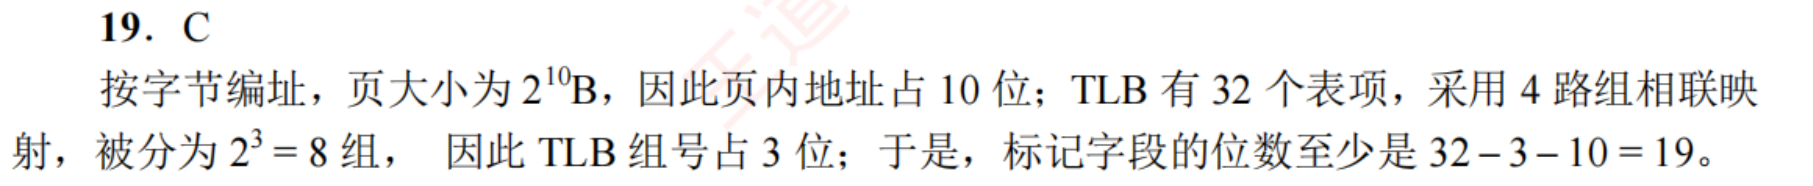
\includegraphics[width=161.13mm,height=180mm,keepaspectratio]{../solutions/assets/6dc401cf7f0e78bb8f73b020.png}\par\smallskip
\par\medskip\Needspace{5\baselineskip}\noindent\hypertarget{a:CO03-E11}{}\label{a:CO03-E11}\textbf{例 3-11}\quad （1）2页、2次缺页，0042 2000H与0042 3000H。（2）以数组元素计，无时间局部性，有空间局部性。（3）块内A4～A0，组号A10～A5；a{[}1{]}{[}0{]}=0042 2100H，组号8。（4）192块；写分配下两种循环均87.5\%。
\par\smallskip
命中率按写分配、无其他数据冲突的模型计算。原题未显式给出写分配，采用非写分配时须重算。

（1）数组 \(24\times64\times4=6144\) B，起址页对齐，覆盖2页。原循环第一次访问第一页a{[}0{]}{[}0{]}、第二页a{[}16{]}{[}0{]}时分别缺页，故障地址为0042 2000H、0042 3000H；页面不置换，共2次。

（2）每元素只写一次，以元素为对象无时间局部性；按行顺序访问相邻元素具有空间局部性。块内复用体现空间局部性。

（3）块长32 B，偏移5位；\(8192/(32\times4)=64\) 组，组号6位，即A10～A5。这些位均在12位页内偏移内，虚实转换保持不变。每行256 B，a{[}1{]}{[}0{]}为0042 2100H，组号 \((\mathtt{2100H}\gg5)\bmod64=8\)。

（4）块数6144/32=192，元素1536。按行每块首次写缺失，随后7次命中，命中率 \(1-192/1536=87.5\%\)。按列时，同一列相邻元素跨8块，24行只映射8组，每组3块，可驻留于4路；后续同块各列继续命中。不同8列批次使用不同组，仍仅192次首次缺失，命中率87.5\%。

\par\medskip\Needspace{5\baselineskip}\noindent\hypertarget{a:CO03-E12}{}\label{a:CO03-E12}\textbf{例 3-12}\quad （1）VPN=A29～A12，偏移=A11～A0。（2）标记=A29～A15，组号=A14～A12。（3）淘汰VPN=4。（4）每表项增加2位。
\par\smallskip
\par\medskip\noindent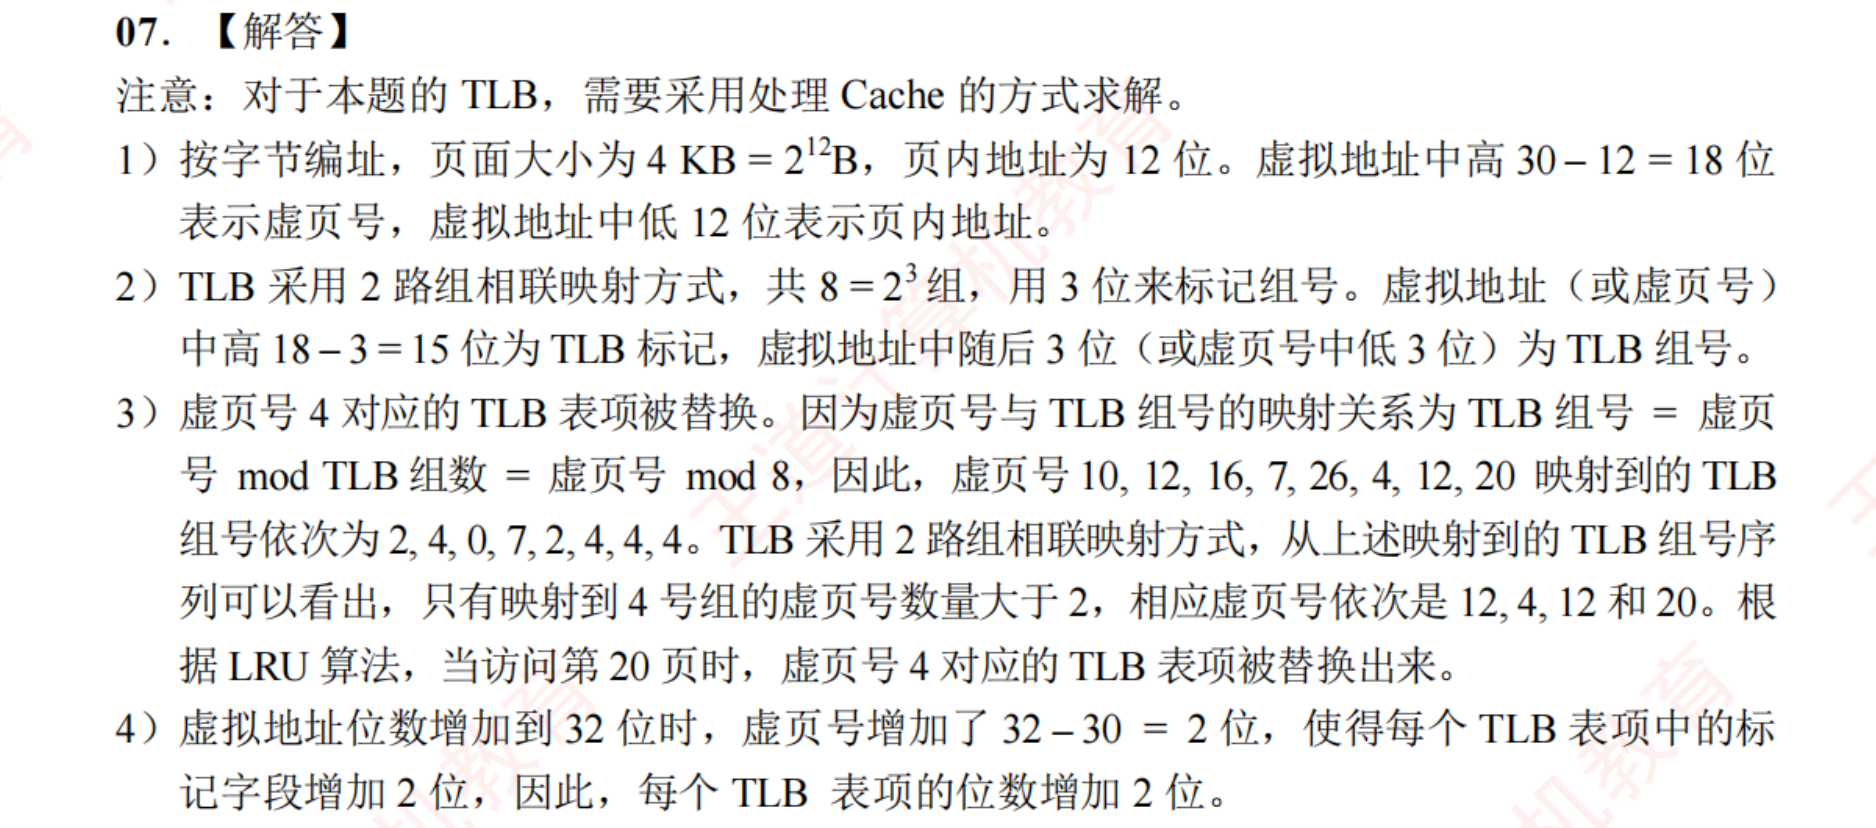
\includegraphics[width=162.00mm,height=180mm,keepaspectratio]{../solutions/assets/9e27e4bcd92e2609a348576a.png}\par\smallskip
\par\medskip\Needspace{5\baselineskip}\noindent\hypertarget{a:CO03-E13}{}\label{a:CO03-E13}\textbf{例 3-13}\quad （1）虚址6/2/6位，物理址6/4/2位。（2）03D4H读得36H；00F1H从主存取数，字节值未知；0229H缺页。
\par\smallskip
（1）64 B页占6位偏移，VPN为8位；TLB16项、4路共4组，组号2位、标记6位。Cache块4 B占2位偏移，16行占4位行号，物理址剩6位标记。

（2）每次均从题给初态开始，查表项时同时检查有效位和标记。

\begin{longtable}[]{@{}
  >{\raggedright\arraybackslash}p{(\columnwidth - 6\tabcolsep) * \real{0.2500}}
  >{\raggedright\arraybackslash}p{(\columnwidth - 6\tabcolsep) * \real{0.2500}}
  >{\raggedright\arraybackslash}p{(\columnwidth - 6\tabcolsep) * \real{0.2500}}
  >{\raggedright\arraybackslash}p{(\columnwidth - 6\tabcolsep) * \real{0.2500}}@{}}
\toprule\noalign{}
\begin{minipage}[b]{\linewidth}\raggedright
虚拟地址
\end{minipage} & \begin{minipage}[b]{\linewidth}\raggedright
VPN／偏移
\end{minipage} & \begin{minipage}[b]{\linewidth}\raggedright
TLB组／标记
\end{minipage} & \begin{minipage}[b]{\linewidth}\raggedright
转换与数据路径
\end{minipage} \\
\midrule\noalign{}
\endhead
\bottomrule\noalign{}
\endlastfoot
03D4H & 0FH／14H & 3／03H & 组3路2命中，页框0DH；物理地址354H；Cache标记0DH、行5H、偏移0，命中读36H \\
00F1H & 03H／31H & 3／00H & TLB缺失，页表P=1、页框02H；物理地址0B1H；Cache标记02H、行CH、偏移1，有效位0，从主存0B0H～0B3H调块后取偏移1，字节值未给出 \\
0229H & 08H／29H & 0／02H & TLB缺失，页表P=0，缺页；待处理并重试后继续 \\
\end{longtable}

第一地址计算为 \(\mathtt{0DH}\times\mathtt{40H}+\mathtt{14H}=\mathtt{354H}\)；第二为 \(\mathtt{02H}\times\mathtt{40H}+\mathtt{31H}=\mathtt{0B1H}\)。第三次在取得驻留页框前进入缺页处理，不继续当前普通数据Cache查找。

\section*{指令系统与 C 程序的机器级表示}
\par\medskip\Needspace{5\baselineskip}\noindent\hypertarget{a:CO04-E01}{}\label{a:CO04-E01}\textbf{例 4-1}\quad D，128条。
\par\smallskip
\par\medskip\noindent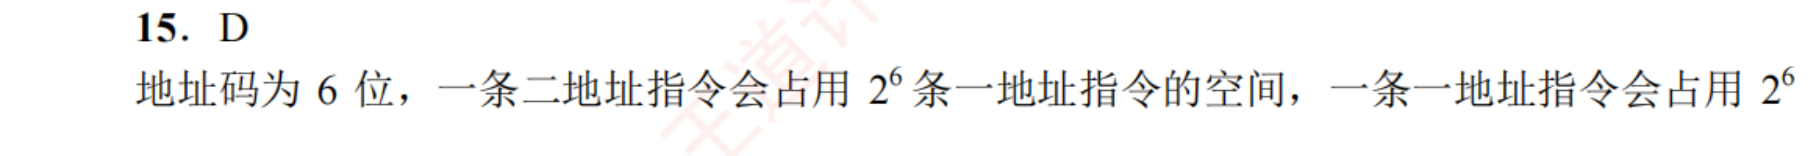
\includegraphics[width=161.13mm,height=180mm,keepaspectratio]{../solutions/assets/8508ee7fd2f2aa5c69c1cb5c.png}\par\smallskip
\par\medskip\noindent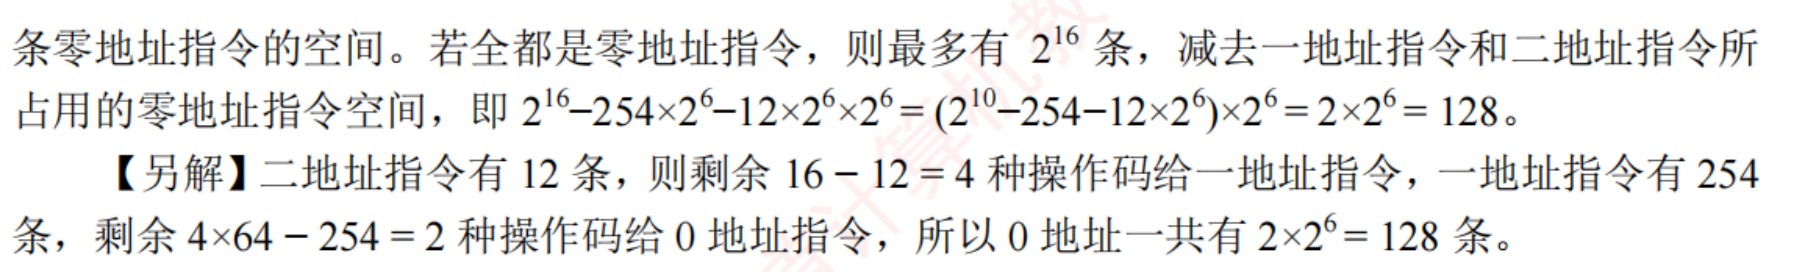
\includegraphics[width=161.13mm,height=180mm,keepaspectratio]{../solutions/assets/173f22c012c076b6d091a8ba.png}\par\smallskip
\par\medskip\Needspace{5\baselineskip}\noindent\hypertarget{a:CO04-E02}{}\label{a:CO04-E02}\textbf{例 4-2}\quad C，2008H。
\par\smallskip
\par\medskip\noindent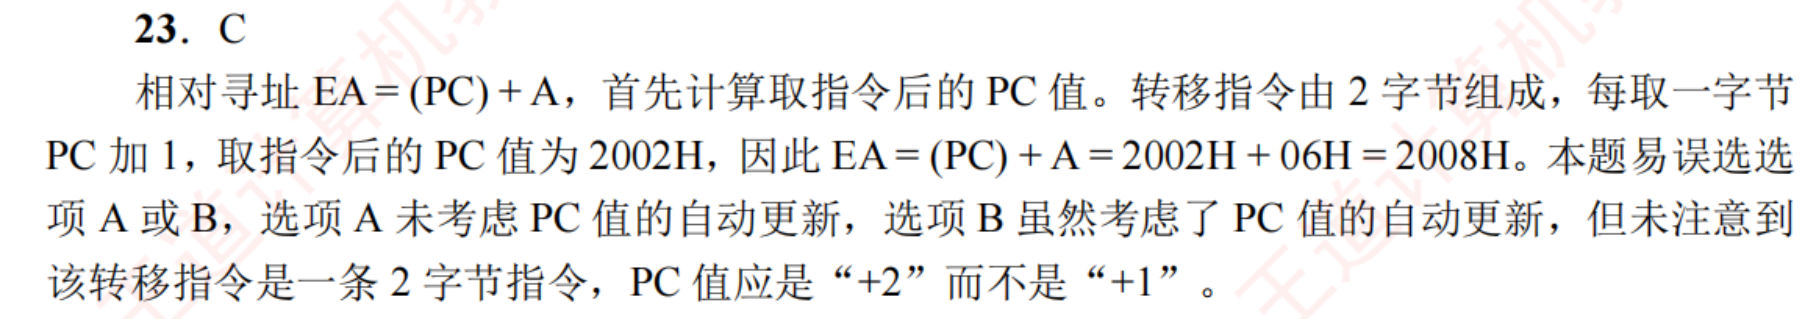
\includegraphics[width=161.13mm,height=180mm,keepaspectratio]{../solutions/assets/063928bd6ca7b59d7c3a1bcf.png}\par\smallskip
\par\medskip\Needspace{5\baselineskip}\noindent\hypertarget{a:CO04-E03}{}\label{a:CO04-E03}\textbf{例 4-3}\quad C。
\par\smallskip
\par\medskip\noindent
\includegraphics[width=161.13mm,height=180mm,keepaspectratio]{../solutions/assets/4915cc2376640eb604d72f1e.png}\par\smallskip
\par\medskip\Needspace{5\baselineskip}\noindent\hypertarget{a:CO04-E04}{}\label{a:CO04-E04}\textbf{例 4-4}\quad A。
\par\smallskip
\par\medskip\noindent
\includegraphics[width=161.13mm,height=180mm,keepaspectratio]{../solutions/assets/ccef9b047a1388d46726db7d.png}\par\smallskip
\par\medskip\Needspace{5\baselineskip}\noindent\hypertarget{a:CO04-E05}{}\label{a:CO04-E05}\textbf{例 4-5}\quad （1）10次，第16行；（2）第12行条件转移，第16、20、30行无条件改变后继；（3）0040102AH，位移−42，小端；（4）32位溢出，改用long long；（5）高32位不等于低32位的符号扩展时OF=1，增加溢出自陷指令。
\par\smallskip
（1）调用参数依次10、9、\ldots、1，共10次（含最外层）。第16行call递归调用，执行9次。

（2）第12行jle为条件转移；第16行call、第20行jmp、第30行ret执行时均改变顺序后继地址。

（3）call占5 B，后继地址为\(00401025\mathrm H+5=0040102A\mathrm H\)。相对位移\(00401000\mathrm H-0040102A\mathrm H=-2A\mathrm H=-42\)，32位补码为FFFF FFD6H。内存低地址先存D6，故为小端。

（4）\(13!>2^{31}-1\)，超出32位int范围。题给机器结果为截低32位：\(6227020800-2^{32}=1932053504\)。标准C有符号溢出规则不保证这种回绕。将返回类型改为至少64位的long long，使递归返回值与乘法均按宽类型计算：

\begin{codeblock}[language={}]
long long f1(int n) {
    if (n > 1) return n * f1(n - 1);
    return 1LL;
}
\end{codeblock}

（5）令精确64位积的高、低32位分别为H、L。当H等于L符号位的32位扩展（L非负则H全0，L负则H全1），OF=0；其他情况OF=1。编译器可在imul后加入检查OF的溢出自陷指令（32位x86为\texttt{into}），OF=1时进入异常处理。

\section*{中央处理器}
\par\medskip\Needspace{5\baselineskip}\noindent\hypertarget{a:CO05-E01}{}\label{a:CO05-E01}\textbf{例 5-1}\quad B。
\par\smallskip
\par\medskip\noindent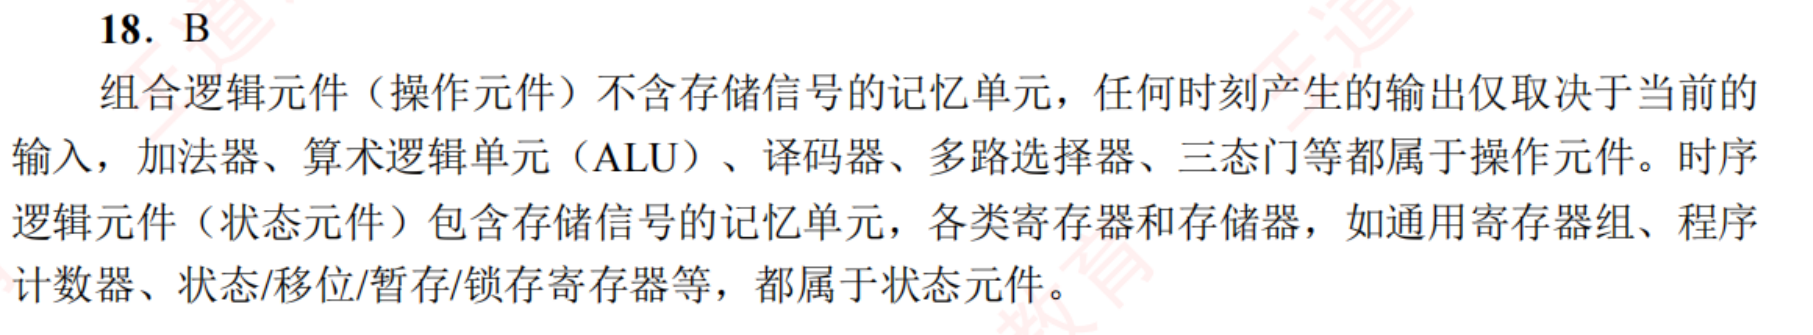
\includegraphics[width=161.13mm,height=180mm,keepaspectratio]{../solutions/assets/b3837d77d8c048bcca15baba.png}\par\smallskip
\par\medskip\Needspace{5\baselineskip}\noindent\hypertarget{a:CO05-E02}{}\label{a:CO05-E02}\textbf{例 5-2}\quad （1）SF=F15，OF见解析；（2）Y保存首操作数，Z暂存结果；（3）16个，来自IR，rd接写地址译码器；（4）PCout/MARin→Read→MDRout/IRin，至少7拍；（5）CU产生，IR和FR提供输入。
\par\smallskip
（1）令\(a=A_{15},b=B_{15},f=F_{15}\)，乘为逻辑与、加为逻辑或： \[
\mathrm{SF}=f,\quad
\mathrm{OF}_{add}=ab\overline f+\overline a\,\overline b f,\quad
\mathrm{OF}_{sub}=a\overline b\,\overline f+\overline a b f.
\] 加法同号输入异号结果时溢出；减法异号输入、结果符号异于A时溢出。

（2）总线同拍仅提供一个值，Y暂存首操作数，随后总线提供第二个。结果先存Z，避免结果与第二输入同时驱动总线，再由Z输出。

（3）rs、rd为4位，可选\(2^4=16\)个寄存器，来自IR字段。rd接写地址译码器，rs控制读多路选择器。

（4）PCout、MARin（1拍）\ensuremath{\to}Read，主存读并送MDR（5拍）\ensuremath{\to}MDRout、IRin（1拍），至少7拍。主存读入MDR已计在5拍内；MDRin为内部总线写MDR，本次主存路径无需该信号。

（5）信号由CU产生，IR的指令信息和FR的状态标志输出连到CU输入。

\par\medskip\Needspace{5\baselineskip}\noindent\hypertarget{a:CO05-E03}{}\label{a:CO05-E03}\textbf{例 5-3}\quad B。
\par\smallskip
\par\medskip\noindent
\includegraphics[width=161.13mm,height=180mm,keepaspectratio]{../solutions/assets/4e5b315842c5c03d793c5989.png}\par\smallskip
\par\medskip\Needspace{5\baselineskip}\noindent\hypertarget{a:CO05-E04}{}\label{a:CO05-E04}\textbf{例 5-4}\quad C，15位。
\par\smallskip
\par\medskip\noindent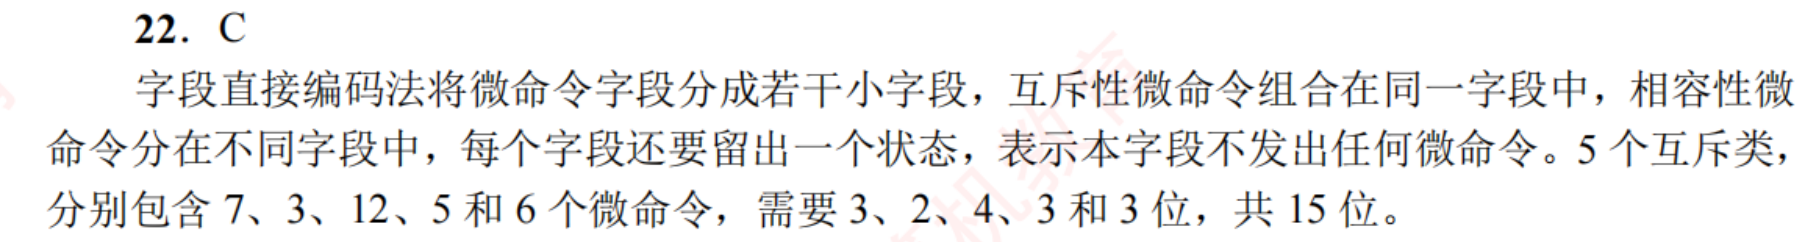
\includegraphics[width=161.13mm,height=180mm,keepaspectratio]{../solutions/assets/ff790becbe50f2d7201875bd.png}\par\smallskip
\par\medskip\Needspace{5\baselineskip}\noindent\hypertarget{a:CO05-E05}{}\label{a:CO05-E05}\textbf{例 5-5}\quad C，8位。
\par\smallskip
\par\medskip\noindent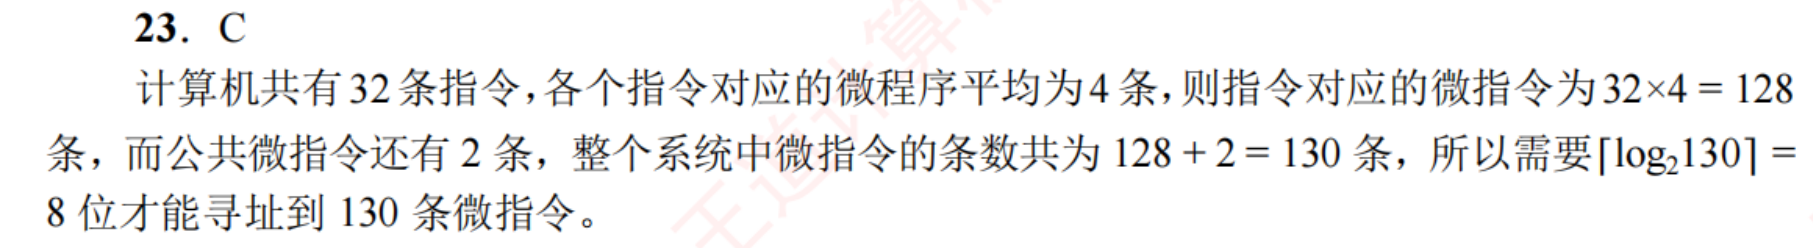
\includegraphics[width=161.13mm,height=180mm,keepaspectratio]{../solutions/assets/a44fd906a7400e824b79fe56.png}\par\smallskip
\par\medskip\Needspace{5\baselineskip}\noindent\hypertarget{a:CO05-E06}{}\label{a:CO05-E06}\textbf{例 5-6}\quad B。
\par\smallskip
\par\medskip\noindent
\includegraphics[width=161.13mm,height=180mm,keepaspectratio]{../solutions/assets/016bffe527117ede4b50a4f5.png}\par\smallskip
\par\medskip\Needspace{5\baselineskip}\noindent\hypertarget{a:CO05-E07}{}\label{a:CO05-E07}\textbf{例 5-7}\quad A，90 ns。
\par\smallskip
共同节拍至少覆盖最慢功能段，\(\tau\ge\max(90,80,70,60)=90\) ns，选A；题目已忽略段寄存器开销。

\par\medskip\Needspace{5\baselineskip}\noindent\hypertarget{a:CO05-E08}{}\label{a:CO05-E08}\textbf{例 5-8}\quad D，1条。
\par\smallskip
无停顿时I2在第5拍MEM末才有r3，I3原本第5拍EX就需使用，需把I3的EX推迟到第6拍。I1的r1已有可用结果，转发可满足。因此插1条NOP，选D。

\par\medskip\Needspace{5\baselineskip}\noindent\hypertarget{a:CO05-E09}{}\label{a:CO05-E09}\textbf{例 5-9}\quad C，I3、I4。
\par\smallskip
\par\medskip\noindent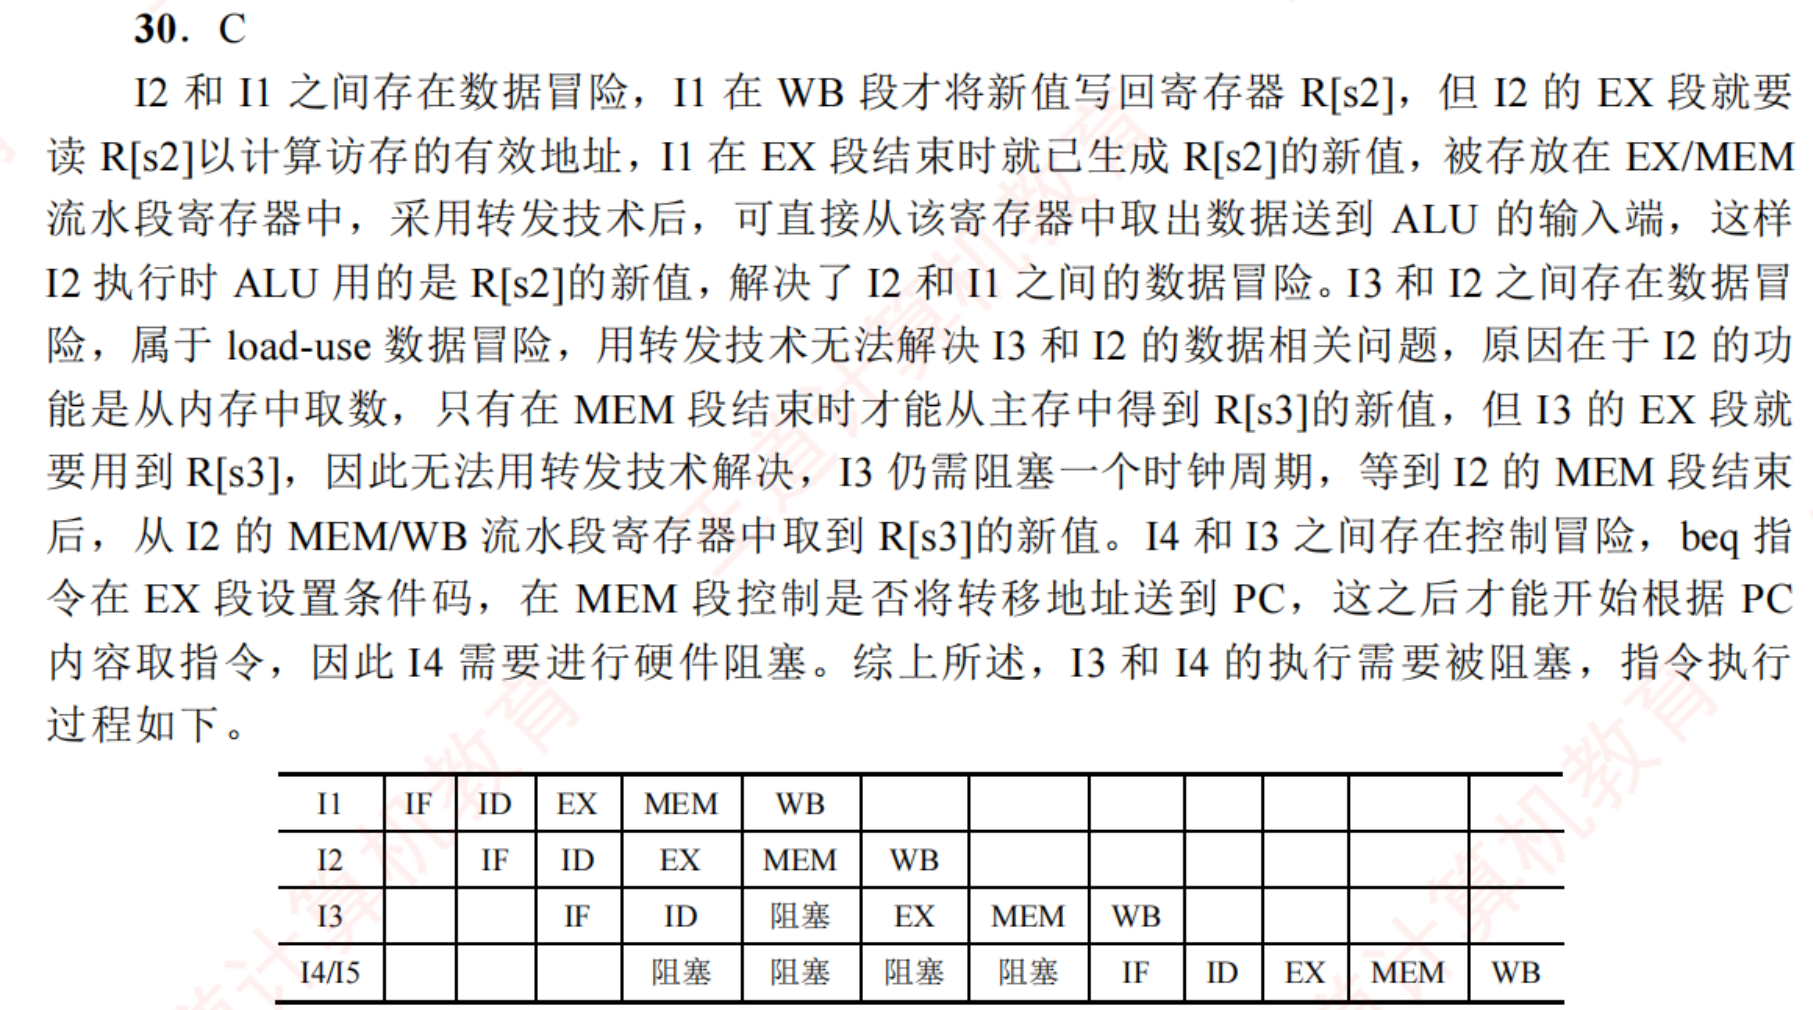
\includegraphics[width=161.13mm,height=180mm,keepaspectratio]{../solutions/assets/54a647a2af8eea60508dbfbf.png}\par\smallskip
\par\medskip\Needspace{5\baselineskip}\noindent\hypertarget{a:CO05-E10}{}\label{a:CO05-E10}\textbf{例 5-10}\quad C。
\par\smallskip
\par\medskip\noindent
\includegraphics[width=161.13mm,height=180mm,keepaspectratio]{../solutions/assets/a67f47b665d8152fe427b79a.png}\par\smallskip
\par\medskip\Needspace{5\baselineskip}\noindent\hypertarget{a:CO05-E11}{}\label{a:CO05-E11}\textbf{例 5-11}\quad （1）FEFFH；（2）8拍；（3）I3等待RAW写回，I4受前级冻结阻塞；（4）至少17拍。
\par\smallskip
统一约束：无转发，同寄存器不能同拍读写，消费者ID最早为生产者WB的下一拍；按题设计所有指令流出五段。

（1）\ensuremath{-}513的16位补码FDFFH，算术右移复制符号位，得到FEFFH（\ensuremath{-}257）。负奇数算术右移按位结果对应向负无穷取整。

（2）\(5+4-1=8\)拍。

（3）I3读R1、R2，分别依赖I1的WB5、I2的WB6，故ID须到第7拍，第4～6拍等待。IF/ID保持使I4也不能取指。I3的WB10后I4最早ID11，因此流出为第14拍。I4的IF阻塞由前级冻结传播产生。

（4）先装x以提前关键链：

\begin{codeblock}[language={}]
I1 LOAD  R1, [x]
I2 LOAD  R2, [a]
I3 SHL   R1
I4 ADD   R1, R2
I5 STORE R2, [x]
\end{codeblock}

\begin{longtable}[]{@{}llllll@{}}
\toprule\noalign{}
指令 & IF & ID成功 & EX & M & WB/流出 \\
\midrule\noalign{}
\endhead
\bottomrule\noalign{}
\endlastfoot
I1 & 1 & 2 & 3 & 4 & 5 \\
I2 & 2 & 3 & 4 & 5 & 6 \\
I3 & 3 & 6 & 7 & 8 & 9 \\
I4 & 6 & 10 & 11 & 12 & 13 \\
I5 & 10 & 14 & 15 & 16 & 17 \\
\end{longtable}

I3在ID端等第4～5拍，I4等第7～9拍，I5等第11～13拍，相应后继取指冻结。x的LOAD\ensuremath{\to}翻倍\ensuremath{\to}相加\ensuremath{\to}STORE链使这三次消费者ID分别至少第6、10、14拍，所列调度达到下界，共17拍。STORE在M16已写主存，按五段流出计为17拍。

\section*{总线}
\par\medskip\Needspace{5\baselineskip}\noindent\hypertarget{a:CO06-E01}{}\label{a:CO06-E01}\textbf{例 6-1}\quad B，20 MB/s。
\par\smallskip
\par\medskip\noindent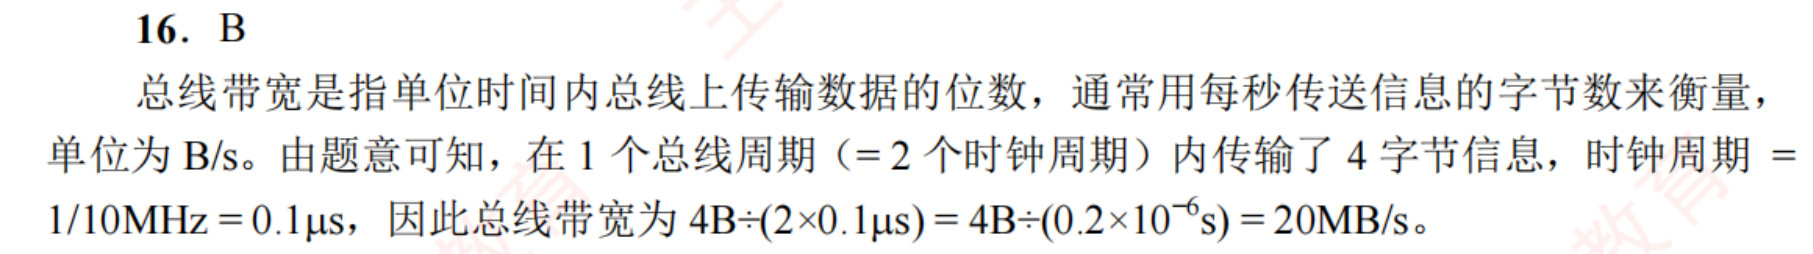
\includegraphics[width=161.13mm,height=180mm,keepaspectratio]{../solutions/assets/fc257258024620931a6bf6fb.png}\par\smallskip
\par\medskip\Needspace{5\baselineskip}\noindent\hypertarget{a:CO06-E02}{}\label{a:CO06-E02}\textbf{例 6-2}\quad 10.664 GB/s；改给333.25 MHz且每拍4次时相同。
\par\smallskip
64位为8 B，\(1333\) MT/s已是每秒传送次数，\(B=1333\times10^6\times8=10.664\) GB/s。若给333.25 MHz，则\(R=4\times333.25=1333\) MT/s，结果相同。

\par\medskip\Needspace{5\baselineskip}\noindent\hypertarget{a:CO06-E03}{}\label{a:CO06-E03}\textbf{例 6-3}\quad D，32 ns。
\par\smallskip
\par\medskip\noindent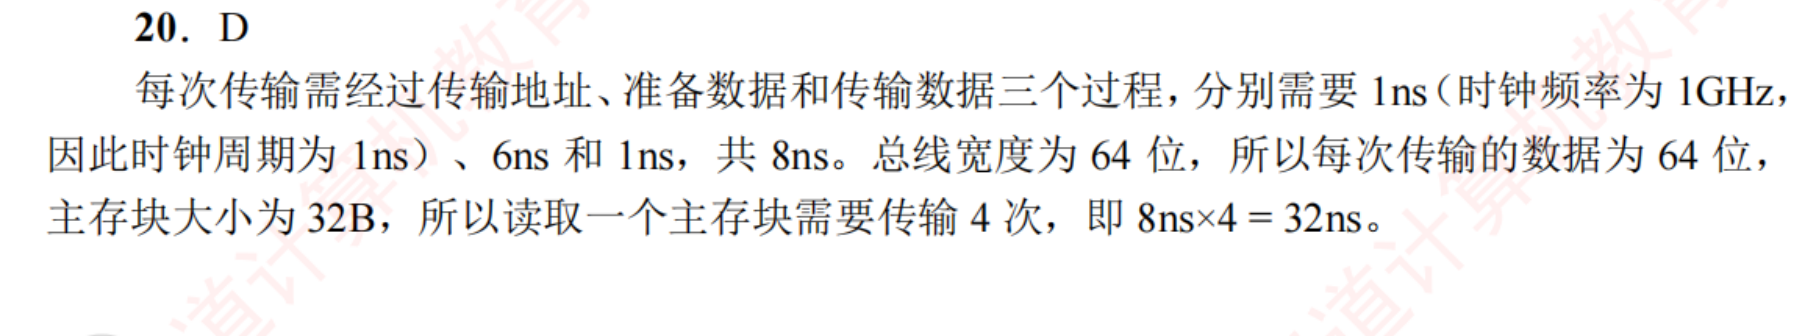
\includegraphics[width=161.13mm,height=180mm,keepaspectratio]{../solutions/assets/0a24c6732153f939bfd6eb58.png}\par\smallskip
\par\medskip\Needspace{5\baselineskip}\noindent\hypertarget{a:CO06-E04}{}\label{a:CO06-E04}\textbf{例 6-4}\quad B，6.72 GB/s。
\par\smallskip
\par\medskip\noindent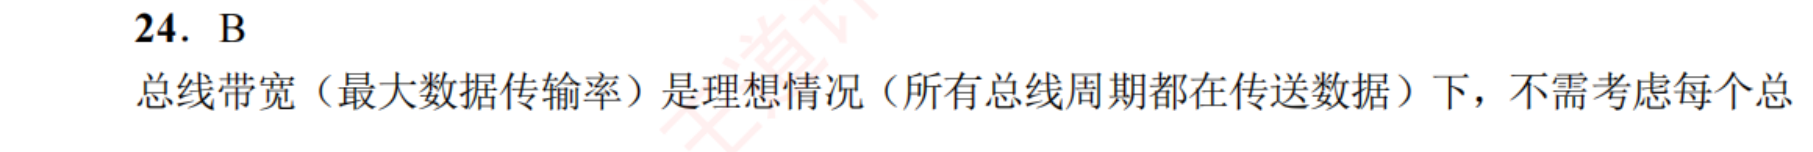
\includegraphics[width=161.13mm,height=180mm,keepaspectratio]{../solutions/assets/6e07a6e55ac755d3360e1df7.png}\par\smallskip
\par\medskip\noindent
\includegraphics[width=161.13mm,height=180mm,keepaspectratio]{../solutions/assets/21ba66d3d9c31d6c38454432.png}\par\smallskip
\section*{输入/输出系统}
\par\medskip\Needspace{5\baselineskip}\noindent\hypertarget{a:CO07-E01}{}\label{a:CO07-E01}\textbf{例 7-1}\quad D。
\par\smallskip
\par\medskip\noindent
\includegraphics[width=161.13mm,height=180mm,keepaspectratio]{../solutions/assets/efd6462f2860f907f9613a65.png}\par\smallskip
\par\medskip\Needspace{5\baselineskip}\noindent\hypertarget{a:CO07-E02}{}\label{a:CO07-E02}\textbf{例 7-2}\quad C，0.20\%。
\par\smallskip
\par\medskip\noindent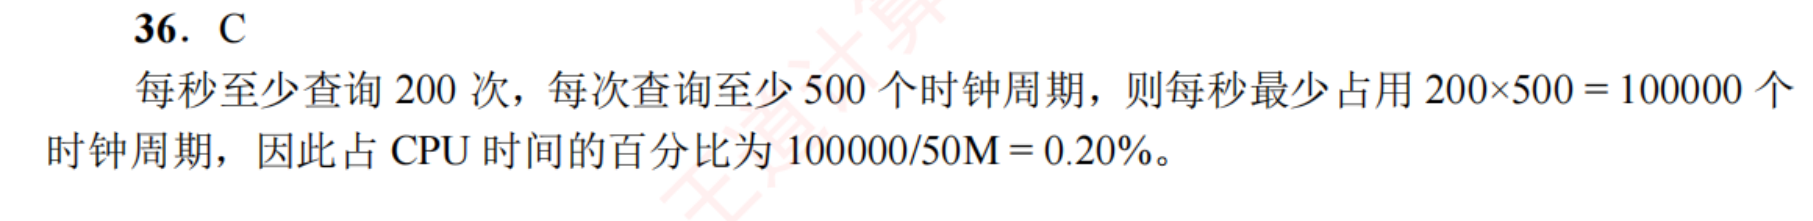
\includegraphics[width=161.13mm,height=180mm,keepaspectratio]{../solutions/assets/7e96f248fbdee2d114583cbd.png}\par\smallskip
\par\medskip\noindent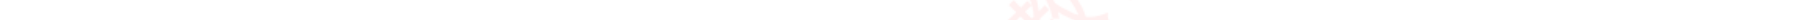
\includegraphics[width=161.13mm,height=180mm,keepaspectratio]{../solutions/assets/296eed924de379b61808f2cf.png}\par\smallskip
\par\medskip\Needspace{5\baselineskip}\noindent\hypertarget{a:CO07-E03}{}\label{a:CO07-E03}\textbf{例 7-3}\quad A、B、C屏蔽字依次100、110、111；开始A→B→C，完成C→B→A。
\par\smallskip
位序A、B、C，1为屏蔽。A允许B、C打断，屏蔽字100；B只允许C，110；C全屏蔽，111。初始均开放，硬件先选A；A开中断后在B、C中先选B，B开中断后进入C。C完成恢复B，B完成恢复A；各层恢复自己的旧屏蔽字，最终按C、B、A完成。

\par\medskip\Needspace{5\baselineskip}\noindent\hypertarget{a:CO07-E04}{}\label{a:CO07-E04}\textbf{例 7-4}\quad B，25\%。
\par\smallskip
\par\medskip\noindent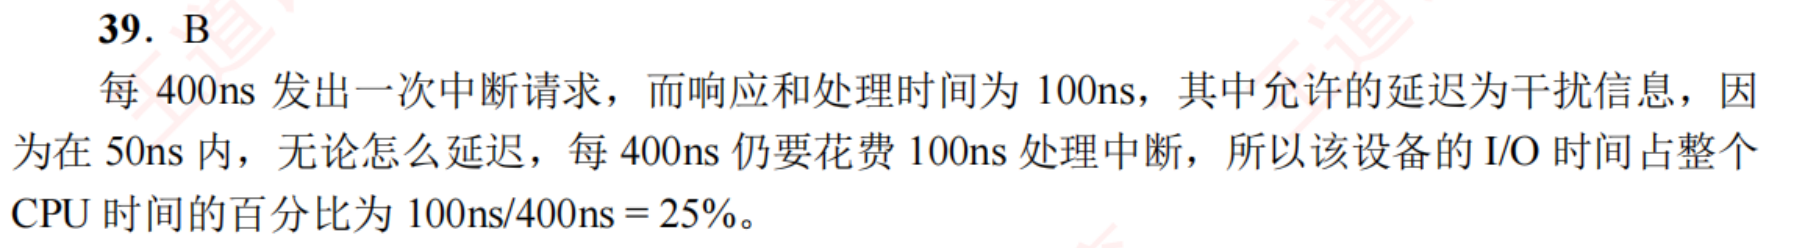
\includegraphics[width=161.13mm,height=180mm,keepaspectratio]{../solutions/assets/23863edf4d7f2fc212f37490.png}\par\smallskip
\par\medskip\Needspace{5\baselineskip}\noindent\hypertarget{a:CO07-E05}{}\label{a:CO07-E05}\textbf{例 7-5}\quad C。
\par\smallskip
\par\medskip\noindent
\includegraphics[width=161.13mm,height=180mm,keepaspectratio]{../solutions/assets/acf89593acfd3532414aadcc.png}\par\smallskip
\par\medskip\Needspace{5\baselineskip}\noindent\hypertarget{a:CO07-E06}{}\label{a:CO07-E06}\textbf{例 7-6}\quad D。
\par\smallskip
\par\medskip\noindent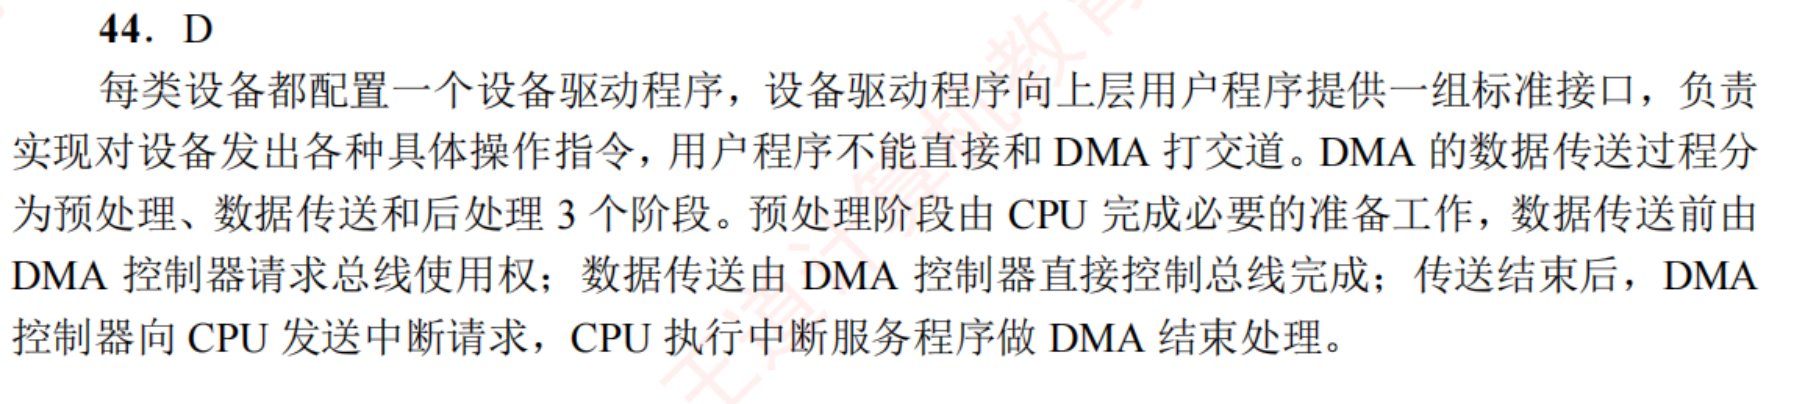
\includegraphics[width=161.13mm,height=180mm,keepaspectratio]{../solutions/assets/c8a7f663ead1cb55f3f8fc5f.png}\par\smallskip
\par\medskip\noindent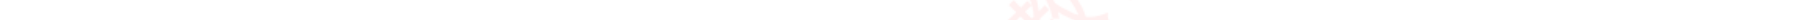
\includegraphics[width=161.13mm,height=180mm,keepaspectratio]{../solutions/assets/8d166b86b7eb09355ca50579.png}\par\smallskip
\par\medskip\Needspace{5\baselineskip}\noindent\hypertarget{a:CO07-E07}{}\label{a:CO07-E07}\textbf{例 7-7}\quad （1）最多2 μs查询一次，至少4\%；（2）不能，需800\%的CPU预算；（3）最多4\%。
\par\smallskip
\par\medskip\noindent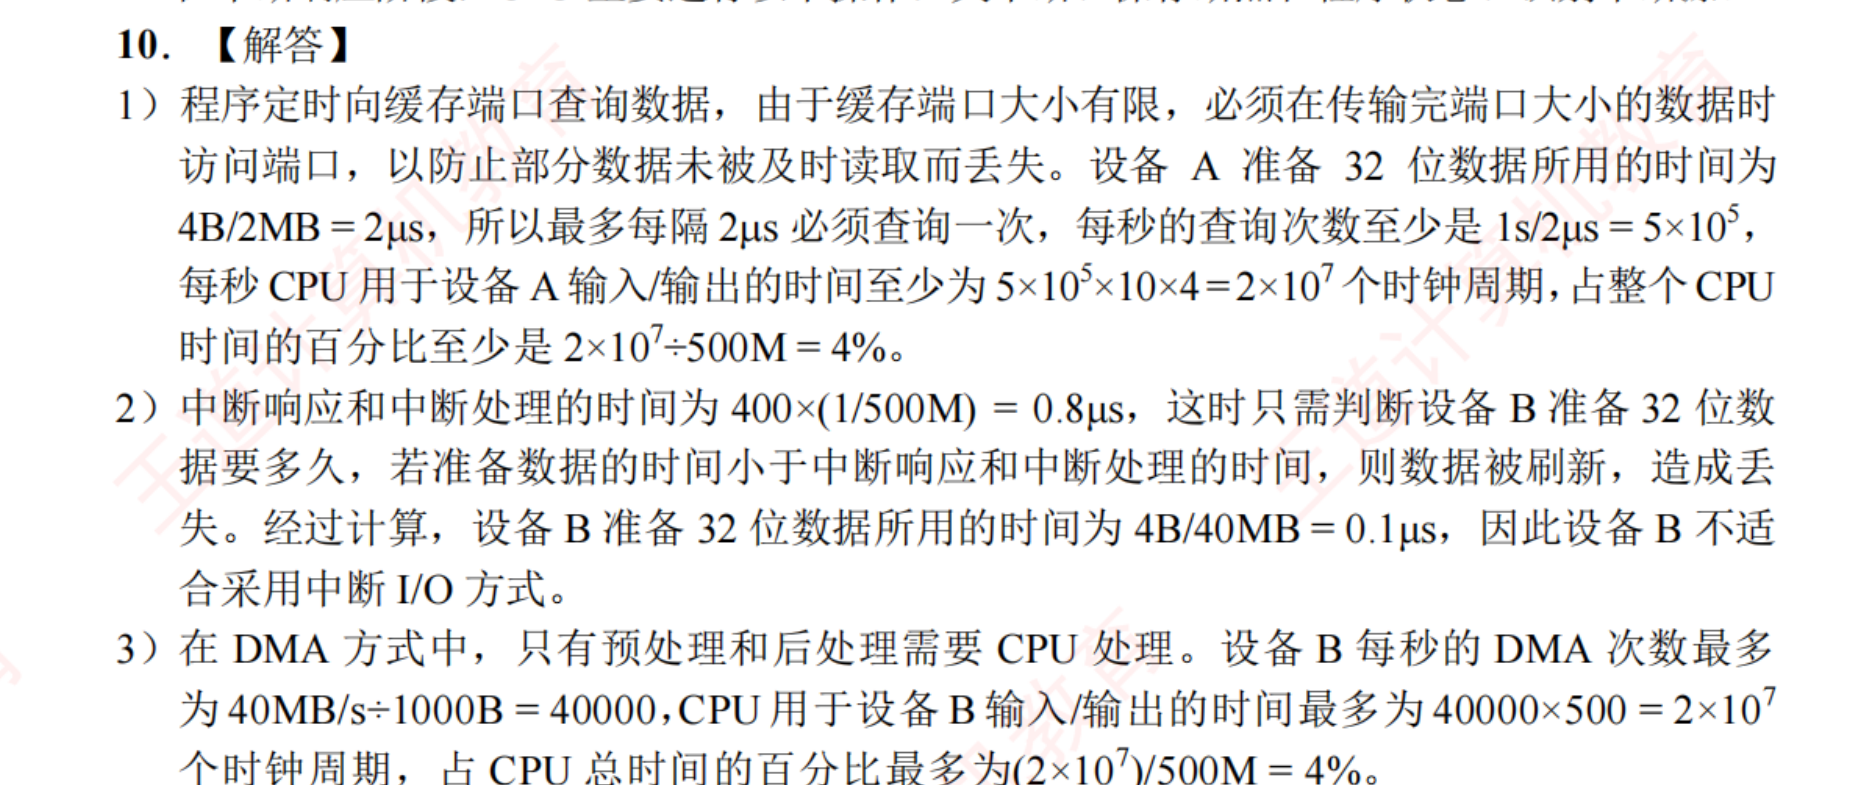
\includegraphics[width=162.00mm,height=180mm,keepaspectratio]{../solutions/assets/cf9f1d23cd9c959b0bbfd684.png}\par\smallskip
\chapter{操作系统}
\section*{计算机系统概述}
\par\medskip\Needspace{5\baselineskip}\noindent\hypertarget{a:OS01-E01}{}\label{a:OS01-E01}\textbf{例 1-1}\quad D
\par\smallskip
\par\medskip\noindent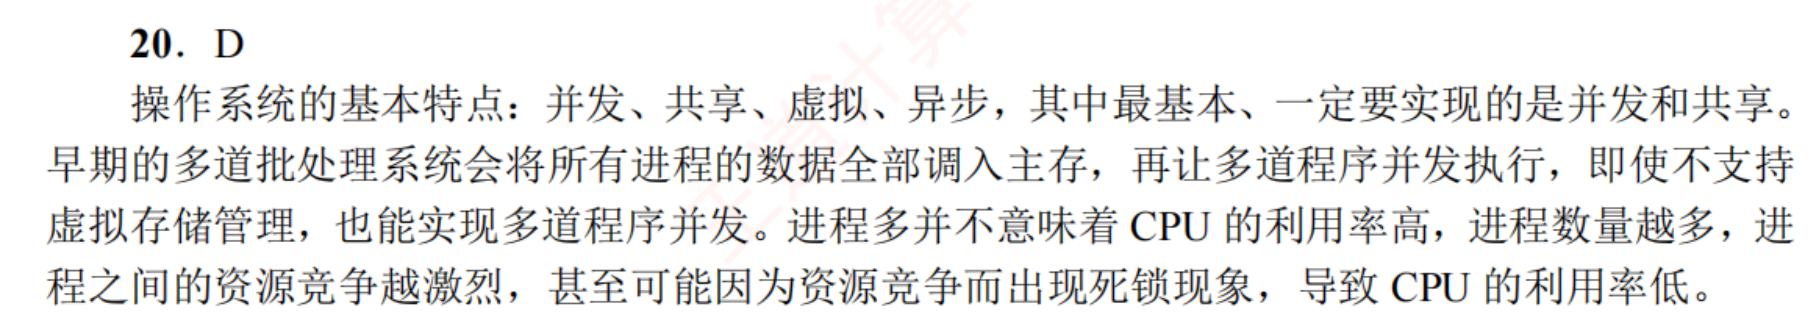
\includegraphics[width=161.13mm,height=180mm,keepaspectratio]{../solutions/assets/fb29814c25288d135b6ceec8.png}\par\smallskip
\par\medskip\Needspace{5\baselineskip}\noindent\hypertarget{a:OS01-E02}{}\label{a:OS01-E02}\textbf{例 1-2}\quad B
\par\smallskip
\par\medskip\noindent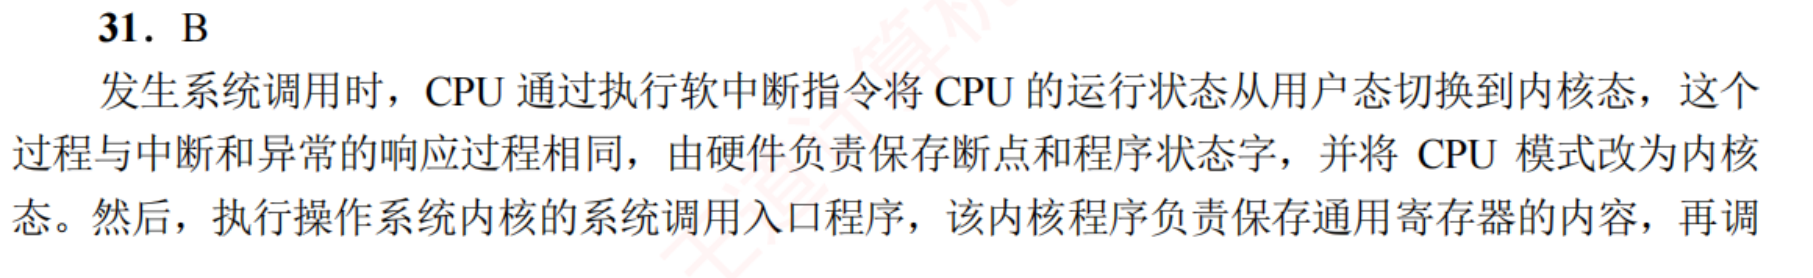
\includegraphics[width=161.13mm,height=180mm,keepaspectratio]{../solutions/assets/2f97943d049f7758959efd93.png}\par\smallskip
\par\medskip\noindent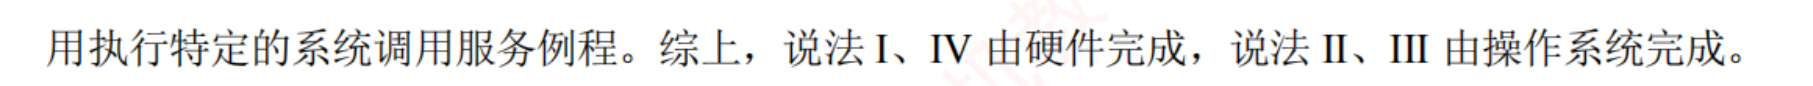
\includegraphics[width=161.13mm,height=180mm,keepaspectratio]{../solutions/assets/f79a14e97ae4d8d87de67bc9.png}\par\smallskip
\par\medskip\Needspace{5\baselineskip}\noindent\hypertarget{a:OS01-E03}{}\label{a:OS01-E03}\textbf{例 1-3}\quad D
\par\smallskip
\par\medskip\noindent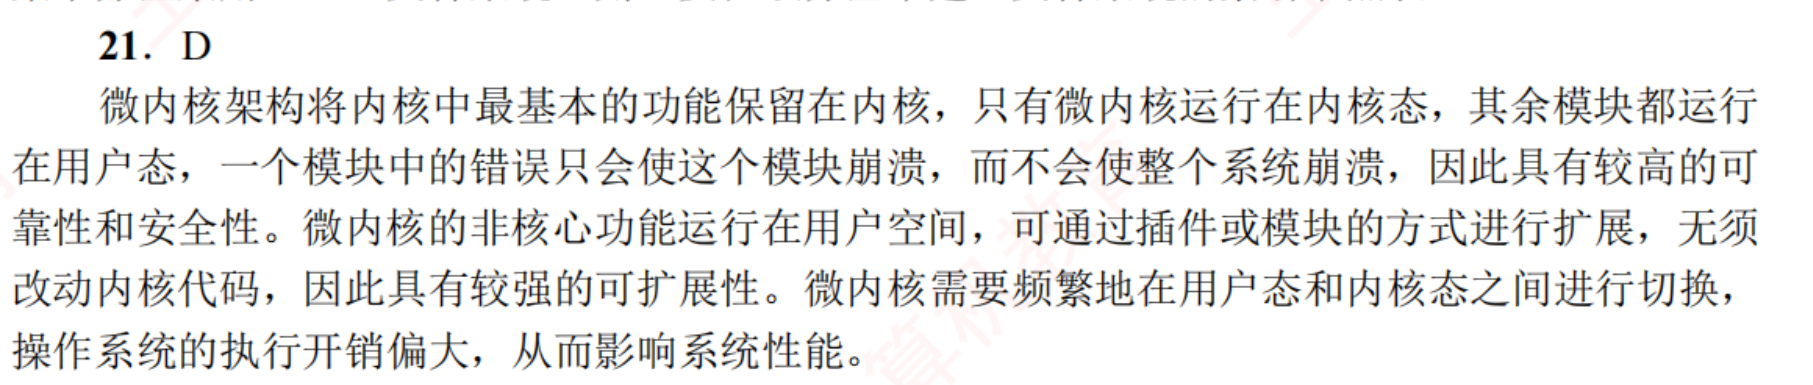
\includegraphics[width=161.13mm,height=180mm,keepaspectratio]{../solutions/assets/2011ccb5a11356314feb6fbe.png}\par\smallskip
\par\medskip\Needspace{5\baselineskip}\noindent\hypertarget{a:OS01-E04}{}\label{a:OS01-E04}\textbf{例 1-4}\quad A
\par\smallskip
\par\medskip\noindent
\includegraphics[width=161.13mm,height=180mm,keepaspectratio]{../solutions/assets/964b3f543a9a3b8c928cd287.png}\par\smallskip
\section*{进程与线程}
\par\medskip\Needspace{5\baselineskip}\noindent\hypertarget{a:OS02-E01}{}\label{a:OS02-E01}\textbf{例 2-1}\quad C
\par\smallskip
\par\medskip\noindent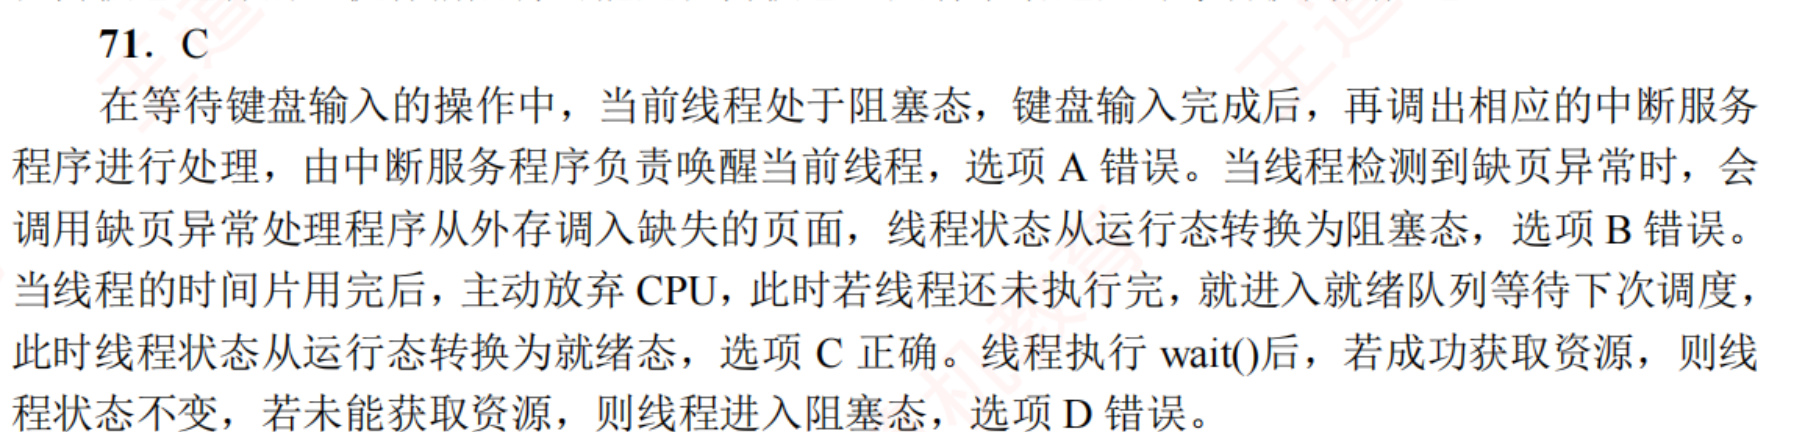
\includegraphics[width=161.13mm,height=180mm,keepaspectratio]{../solutions/assets/25ce26c36e7c482a40edbe64.png}\par\smallskip
\par\medskip\Needspace{5\baselineskip}\noindent\hypertarget{a:OS02-E02}{}\label{a:OS02-E02}\textbf{例 2-2}\quad D
\par\smallskip
\par\medskip\noindent
\includegraphics[width=161.13mm,height=180mm,keepaspectratio]{../solutions/assets/acc422dbd29081ddb703b090.png}\par\smallskip
\par\medskip\Needspace{5\baselineskip}\noindent\hypertarget{a:OS02-E03}{}\label{a:OS02-E03}\textbf{例 2-3}\quad B；61 ms
\par\smallskip
\par\medskip\noindent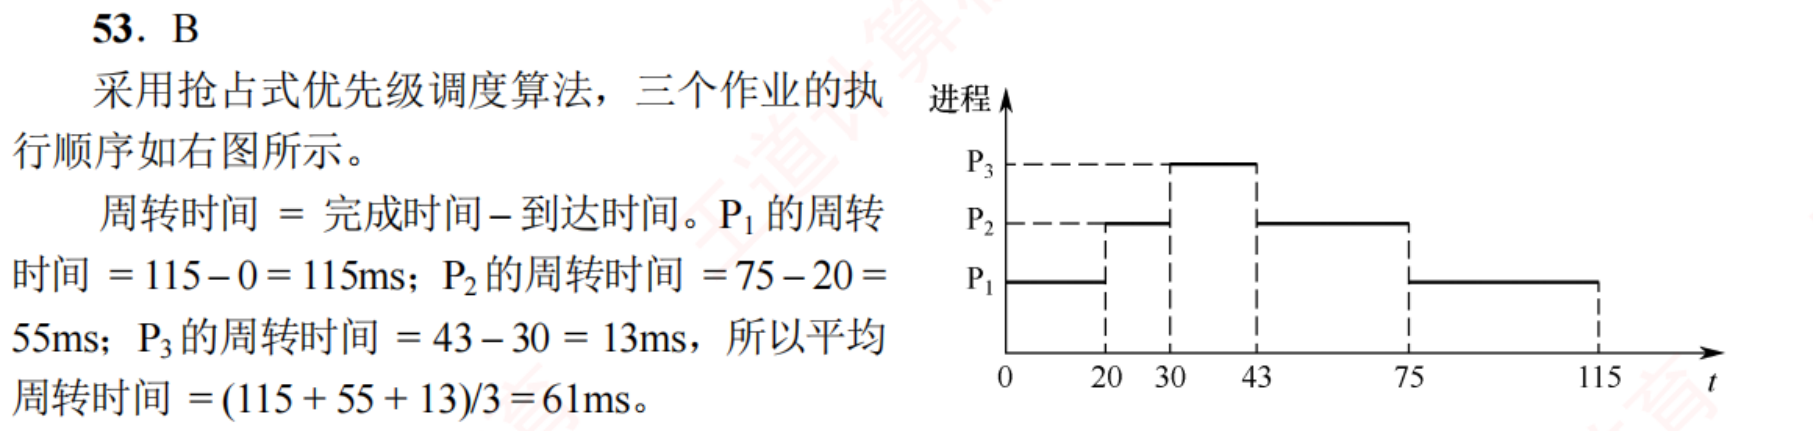
\includegraphics[width=161.13mm,height=180mm,keepaspectratio]{../solutions/assets/607303d5d58f325d5ce9aebe.png}\par\smallskip
\par\medskip\Needspace{5\baselineskip}\noindent\hypertarget{a:OS02-E04}{}\label{a:OS02-E04}\textbf{例 2-4}\quad C；6次
\par\smallskip
\par\medskip\noindent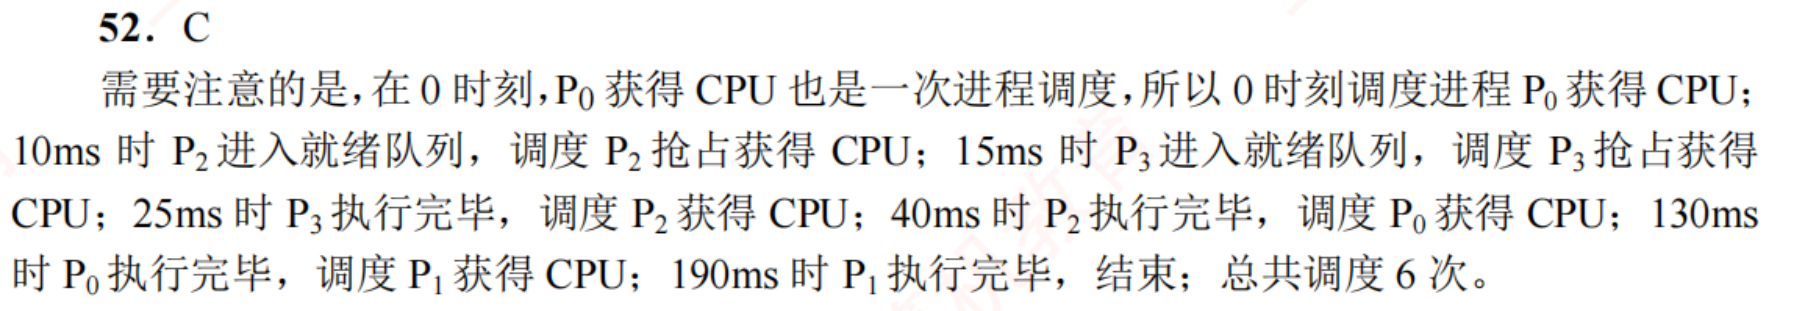
\includegraphics[width=161.13mm,height=180mm,keepaspectratio]{../solutions/assets/38eb76f35d777674fa695020.png}\par\smallskip
\par\medskip\Needspace{5\baselineskip}\noindent\hypertarget{a:OS02-E05}{}\label{a:OS02-E05}\textbf{例 2-5}\quad C；15 ms
\par\smallskip
\par\medskip\noindent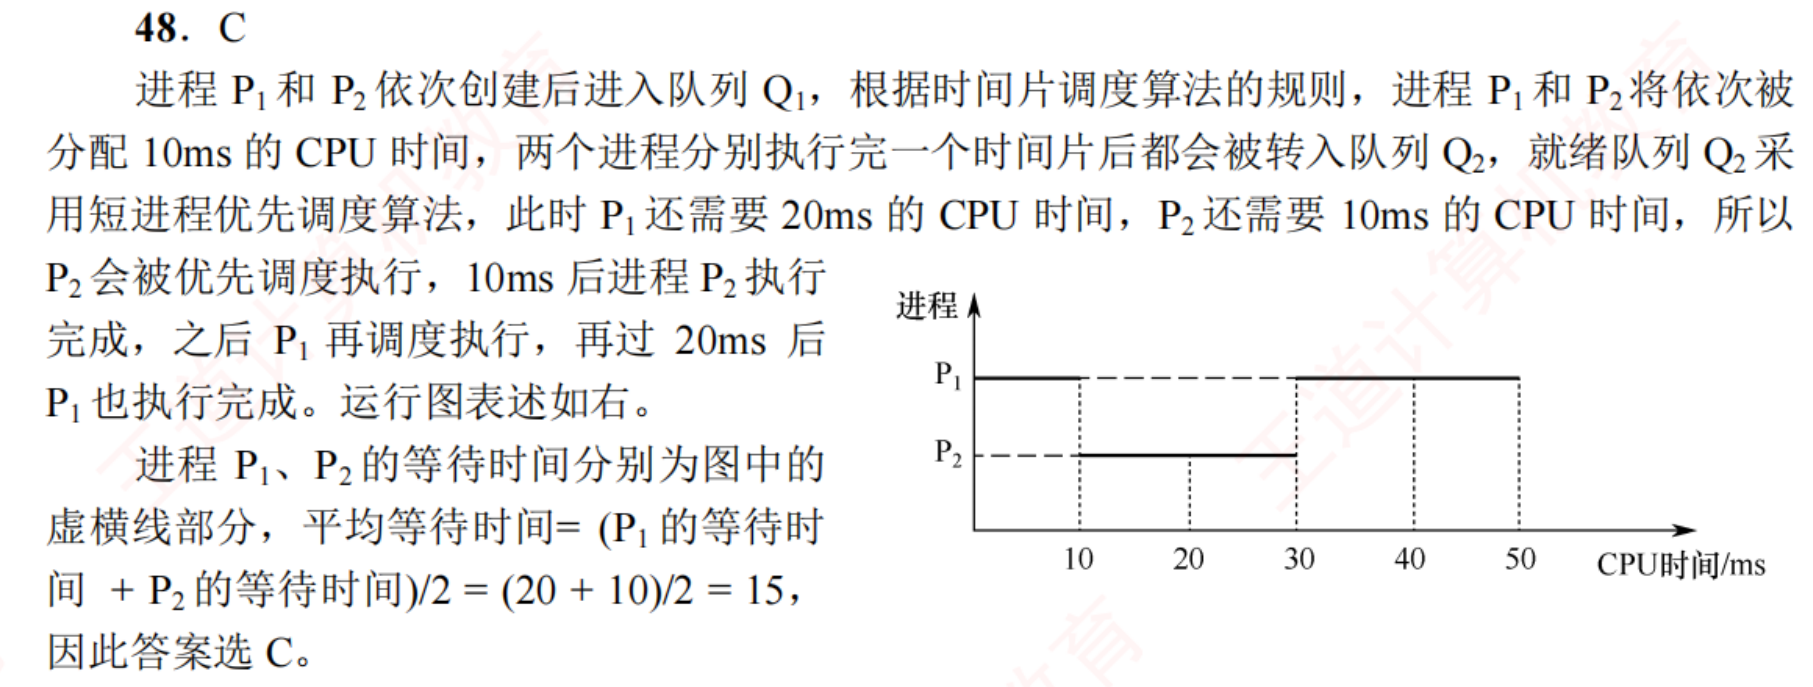
\includegraphics[width=161.13mm,height=180mm,keepaspectratio]{../solutions/assets/2901fb362667ecdf0e7ee754.png}\par\smallskip
\par\medskip\Needspace{5\baselineskip}\noindent\hypertarget{a:OS02-E06}{}\label{a:OS02-E06}\textbf{例 2-6}\quad SRTF：13；RR：19.25
\par\smallskip
\par\medskip\noindent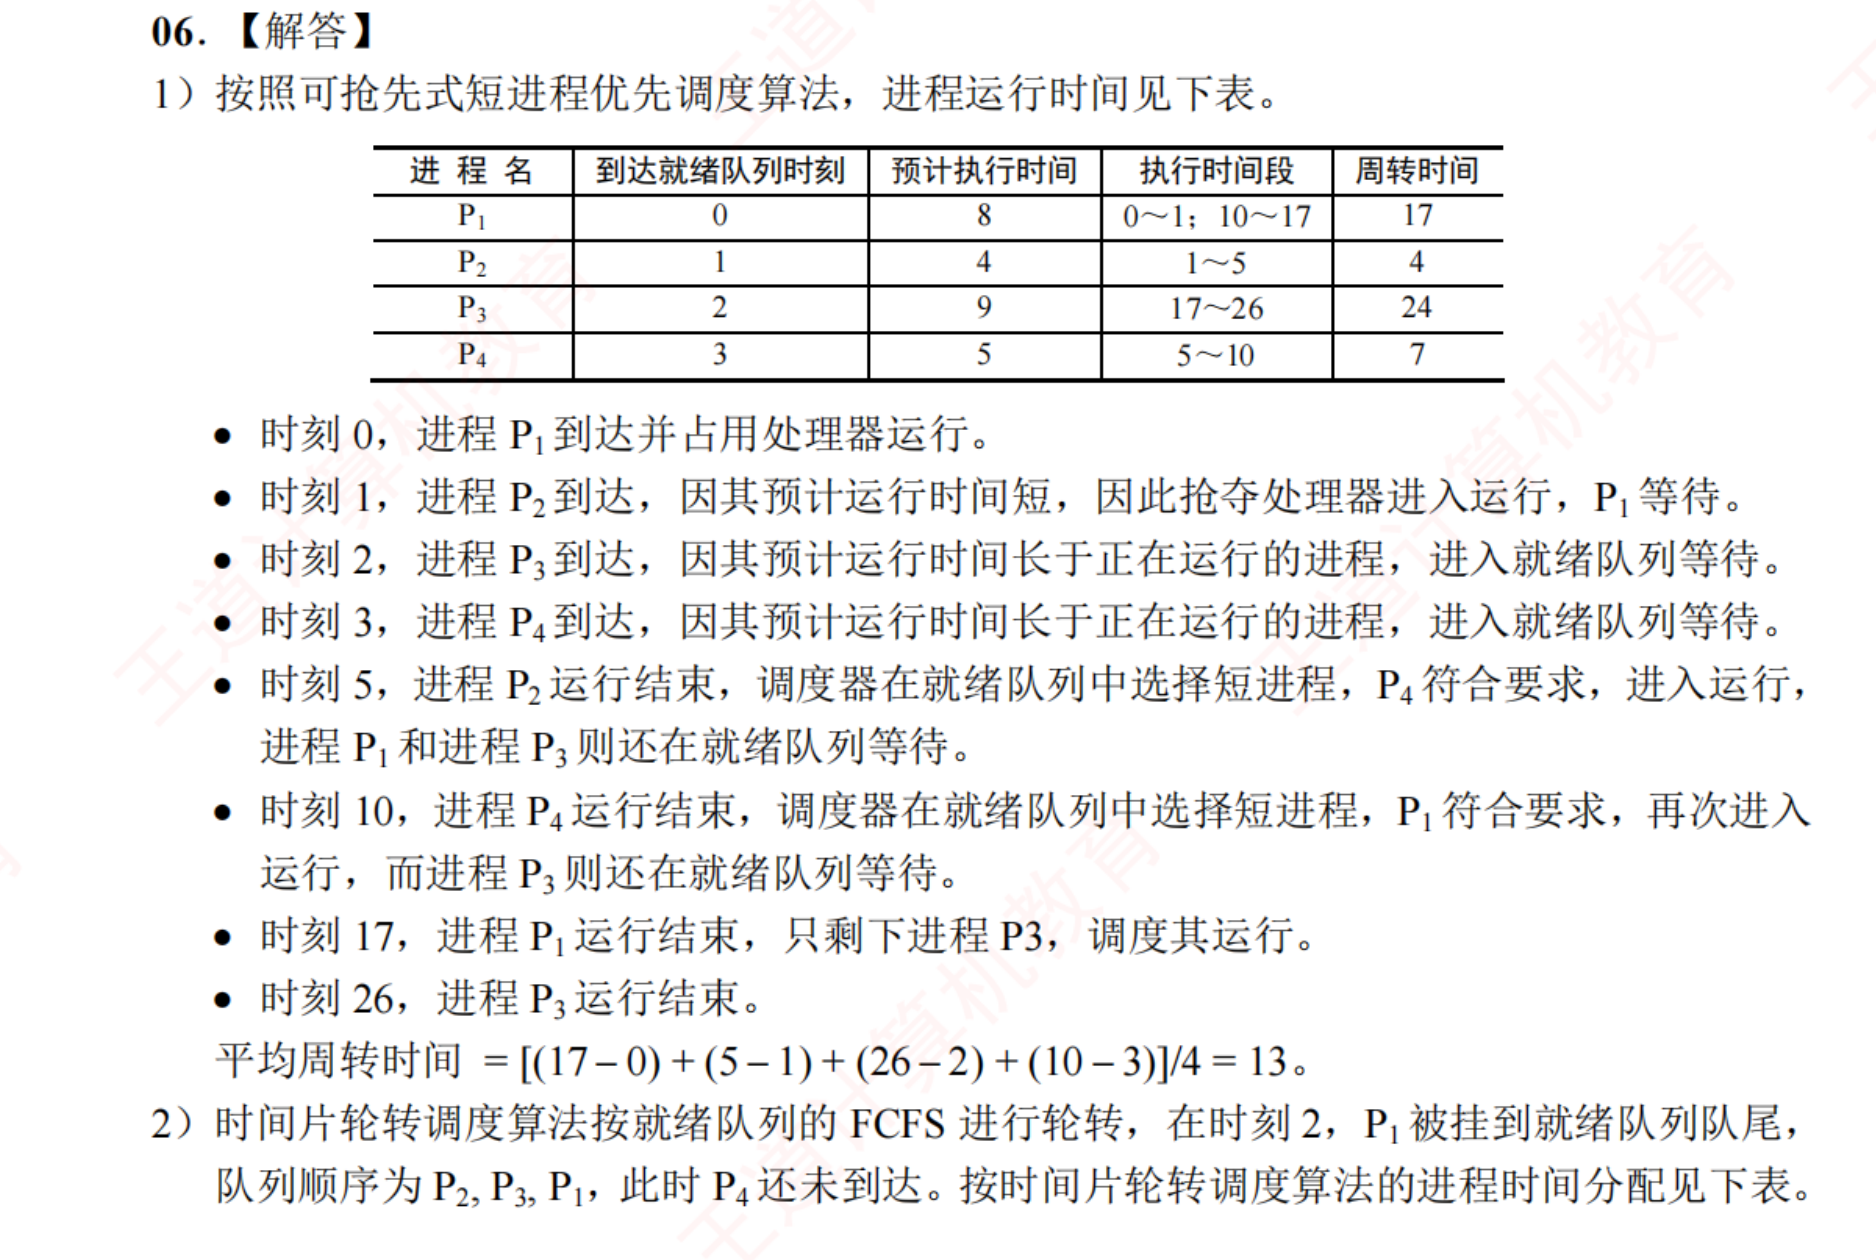
\includegraphics[width=162.00mm,height=180mm,keepaspectratio]{../solutions/assets/ba1d956c4558c5a9b60a5214.png}\par\smallskip
\par\medskip\noindent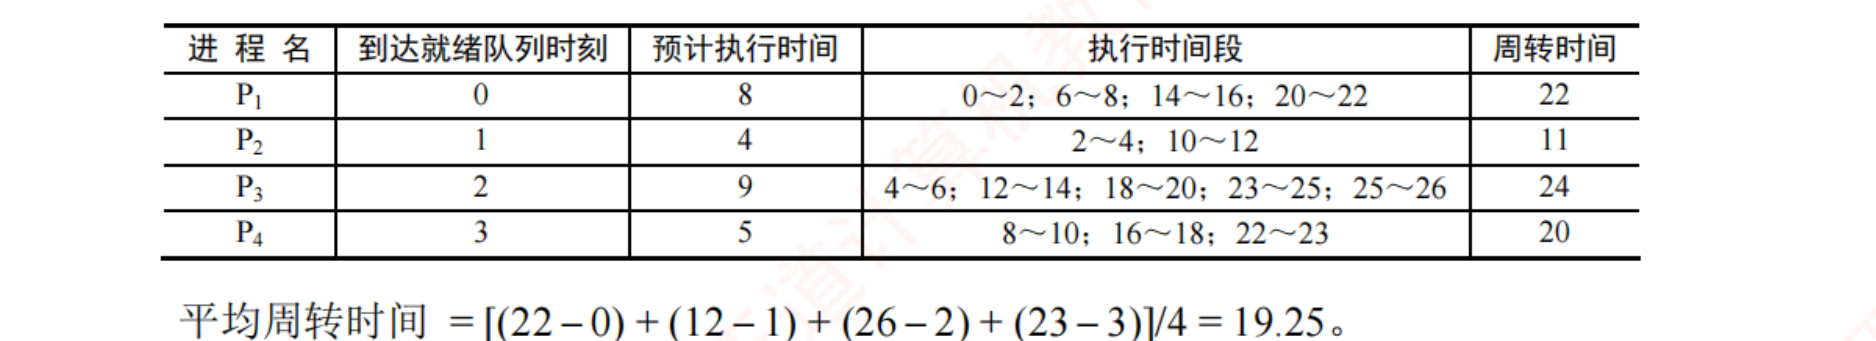
\includegraphics[width=162.00mm,height=180mm,keepaspectratio]{../solutions/assets/a1058747dccc556ae1ea1530.png}\par\smallskip
\par\medskip\Needspace{5\baselineskip}\noindent\hypertarget{a:OS02-E07}{}\label{a:OS02-E07}\textbf{例 2-7}\quad \(priority=nice+k_1cpuTime-k_2waitTime\)，\(k_1,k_2>0\)
\par\smallskip
（1）只比较 nice 时，较小 nice 的进程持续就绪可使较大 nice 的进程长期落选。

（2）取 \(priority=nice+k_1cpuTime-k_2waitTime\)，\(k_1,k_2>0\)。运行使优先数增大，等待使优先数减小；waitTime 实现老化。按题设在运行时清 waitTime、就绪时清 cpuTime。无饥饿保证还需有限进程或有界 nice、持续重算、适当抢占或有限运行段及公平同级处理等前提。

\par\medskip\Needspace{5\baselineskip}\noindent\hypertarget{a:OS02-E08}{}\label{a:OS02-E08}\textbf{例 2-8}\quad C
\par\smallskip
\par\medskip\noindent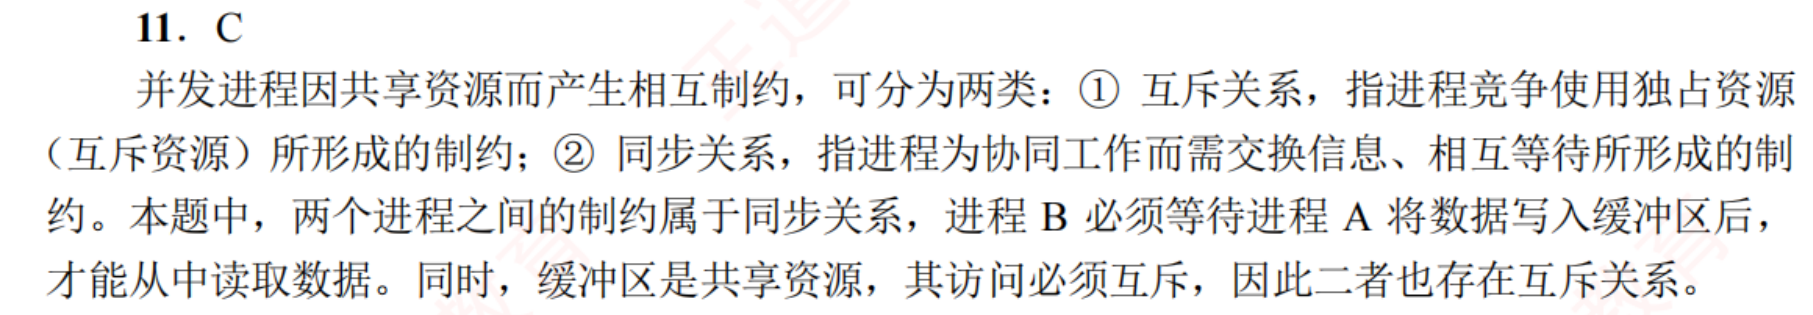
\includegraphics[width=161.13mm,height=180mm,keepaspectratio]{../solutions/assets/f683e73ca0a3c8f9aa0ef47e.png}\par\smallskip
\par\medskip\Needspace{5\baselineskip}\noindent\hypertarget{a:OS02-E09}{}\label{a:OS02-E09}\textbf{例 2-9}\quad D
\par\smallskip
\par\medskip\noindent
\includegraphics[width=161.13mm,height=180mm,keepaspectratio]{../solutions/assets/01171a1d495fca30b98b481b.png}\par\smallskip
\par\medskip\Needspace{5\baselineskip}\noindent\hypertarget{a:OS02-E10}{}\label{a:OS02-E10}\textbf{例 2-10}\quad 两个信号量，初值均0
\par\smallskip
T1 按 A、E、F 执行，T2 按 B、C、D 执行；本线程顺序已保证 B\ensuremath{\to}C、C\ensuremath{\to}D、E\ensuremath{\to}F。跨线程只需 A\ensuremath{\to}C 和 C\ensuremath{\to}E。

\begin{codeblock}[language={}]
semaphore ac=0, ce=0;
T1: A; V(ac); P(ce); E; F;
T2: B; P(ac); C; V(ce); D;
\end{codeblock}

C 前已完成本线程的 B 并收到 A 通知；E 前收到 C 通知。V(ce) 放在 C 后、D 前，保留 D 与 E/F 的并发。

\par\medskip\Needspace{5\baselineskip}\noindent\hypertarget{a:OS02-E11}{}\label{a:OS02-E11}\textbf{例 2-11}\quad （1）是；（2）done=0；（3）mutex=1
\par\smallskip
（1）两个 C1 可同时发现空缓冲并互相覆盖，检查和写入须作为临界区保护。

（2）初始空且各执行一次，只需写完通知：

\begin{codeblock}[language={}]
semaphore done=0;
P1: C1; V(done);
P2: P(done); C2;
\end{codeblock}

该先后关系已排除两次操作重叠。

（3）初始非空且两次修改均不清空，使用互斥量：

\begin{codeblock}[language={}]
semaphore mutex=1;
P1: P(mutex); C3; V(mutex);
P2: P(mutex); C3; V(mutex);
\end{codeblock}

每问按各自初态和活动范围独立分析。

\par\medskip\Needspace{5\baselineskip}\noindent\hypertarget{a:OS02-E12}{}\label{a:OS02-E12}\textbf{例 2-12}\quad empty=N，odd=even=0，mutex=1；按类别发布
\par\smallskip
原题未明确初态，沿参考解取初始为空；有初存 a 个奇数、b 个偶数时改为 empty=N-a-b、odd=a、even=b。所有缓冲放取共用 mutex；奇偶分别计产品许可。

\begin{codeblock}[language={}]
semaphore empty=N, odd=0, even=0, mutex=1;
P1: while (true) {
    x=produce();
    P(empty); P(mutex); put(); V(mutex);
    if (x%2) V(odd); else V(even);
}
P2: while (true) {
    P(odd); P(mutex); getodd(); V(mutex);
    V(empty); countodd();
}
P3: while (true) {
    P(even); P(mutex); geteven(); V(mutex);
    V(empty); counteven();
}
\end{codeblock}

put() 放入 P1 当前的本地整数 x。实际取出后立即归还空位，私有统计留在锁外；某类长期不产生时，该消费者可一直等，其他进程仍可推进。

\par\medskip\Needspace{5\baselineskip}\noindent\hypertarget{a:OS02-E13}{}\label{a:OS02-E13}\textbf{例 2-13}\quad empty=1000，full=0，mutex=batch=1
\par\smallskip
mutex 保护单次缓冲操作及指针，batch 保证一个消费者连续取10件；生产者不申请 batch。

\begin{codeblock}[language={}]
semaphore empty=1000, full=0, mutex=1, batch=1;
item buf[1000]; int in=0, out=0;
producer: while (true) {
    x=produce(); P(empty); P(mutex);
    buf[in]=x; in=(in+1)%1000;
    V(mutex); V(full);
}
consumer: while (true) {
    P(batch);
    for (int k=0; k<10; k++) {
        P(full); P(mutex);
        local[k]=buf[out]; out=(out+1)%1000;
        V(mutex); V(empty);
    }
    V(batch); consume(local);
}
\end{codeblock}

消费者缺货时只持 batch、等待 full，生产者仍可取得 mutex 补货；其他消费者无法插入。每取一件即归还空位，整批无须在开始时凑齐。

\par\medskip\Needspace{5\baselineskip}\noindent\hypertarget{a:OS02-E14}{}\label{a:OS02-E14}\textbf{例 2-14}\quad D
\par\smallskip
\par\medskip\noindent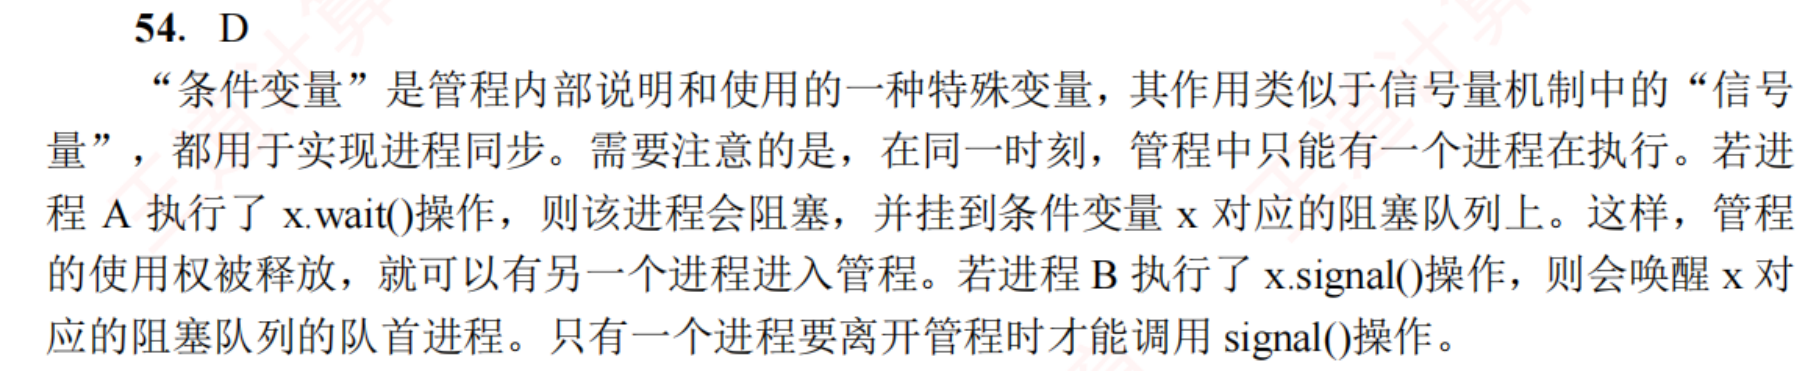
\includegraphics[width=161.13mm,height=180mm,keepaspectratio]{../solutions/assets/57fff1b9d9b5e5c372977afe.png}\par\smallskip
\par\medskip\Needspace{5\baselineskip}\noindent\hypertarget{a:OS02-E15}{}\label{a:OS02-E15}\textbf{例 2-15}\quad B
\par\smallskip
\par\medskip\noindent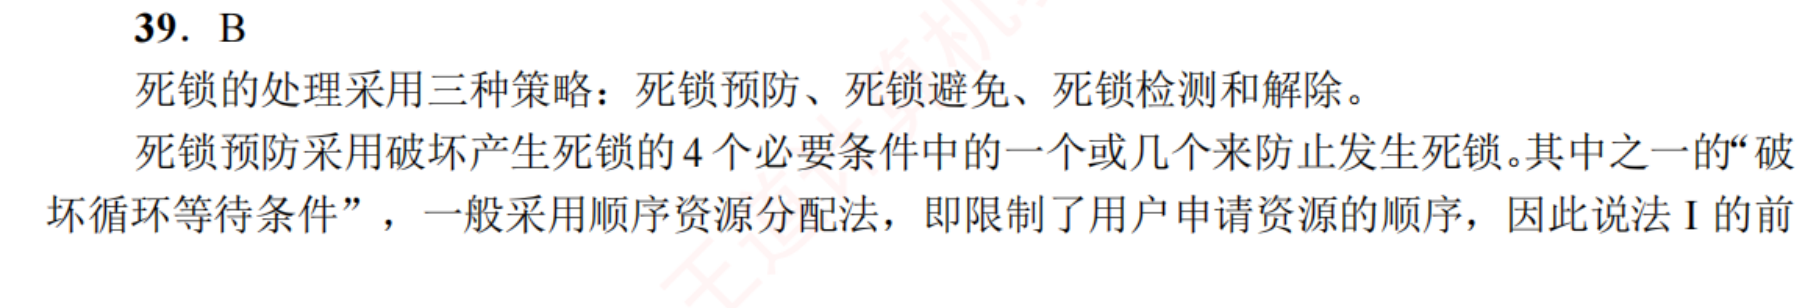
\includegraphics[width=161.13mm,height=180mm,keepaspectratio]{../solutions/assets/74df1f490b2b10218fed0ac4.png}\par\smallskip
\par\medskip\noindent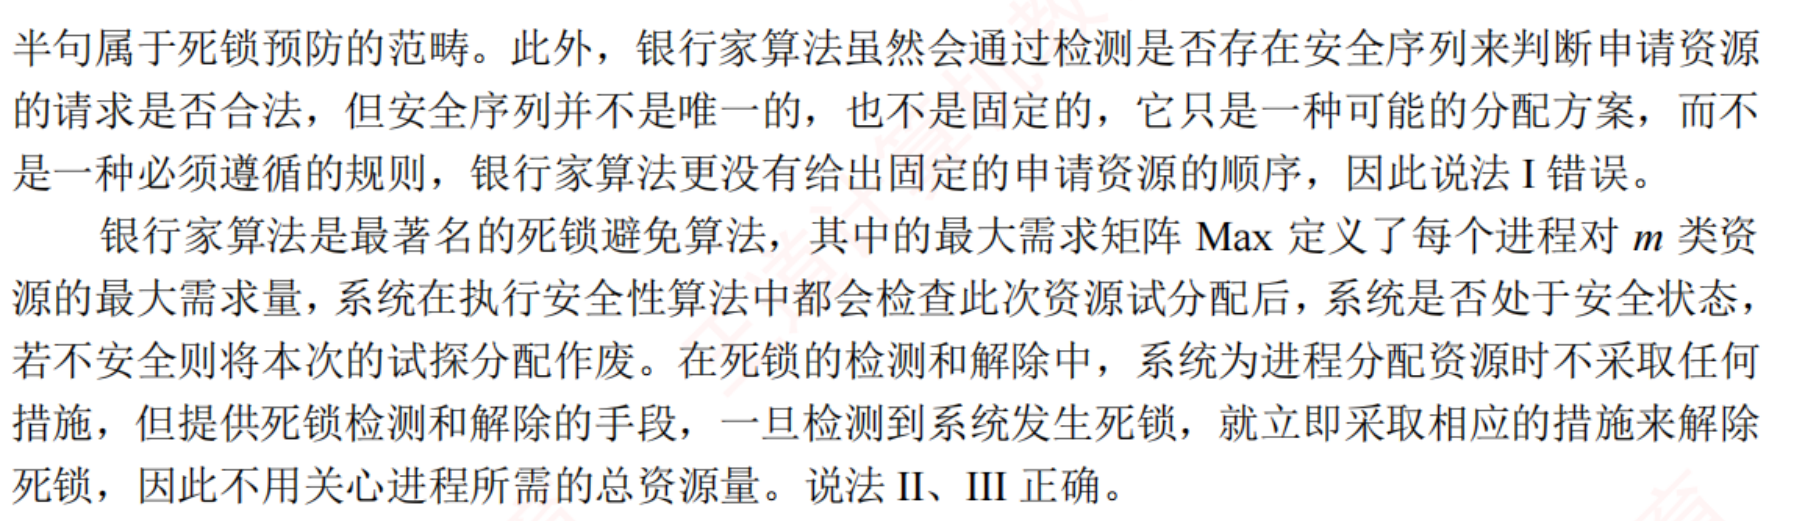
\includegraphics[width=161.13mm,height=180mm,keepaspectratio]{../solutions/assets/a2b691e5a78d91268c17cb95.png}\par\smallskip
\par\medskip\Needspace{5\baselineskip}\noindent\hypertarget{a:OS02-E16}{}\label{a:OS02-E16}\textbf{例 2-16}\quad D；不存在安全序列
\par\smallskip
Work 初为 \((0,2,1)\)，仅 P1 可完成，回收后为 \((2,2,1)\)；再选 P4 后为 \((2,2,2)\)。P2、P3 均仍需3个 R2，仅2个可用，无法继续。完成前两人无法证明整个系统安全；实际当前请求未给出，不能据此确定已死锁。

\par\medskip\Needspace{5\baselineskip}\noindent\hypertarget{a:OS02-E17}{}\label{a:OS02-E17}\textbf{例 2-17}\quad C；仅Ⅰ
\par\smallskip
\par\medskip\noindent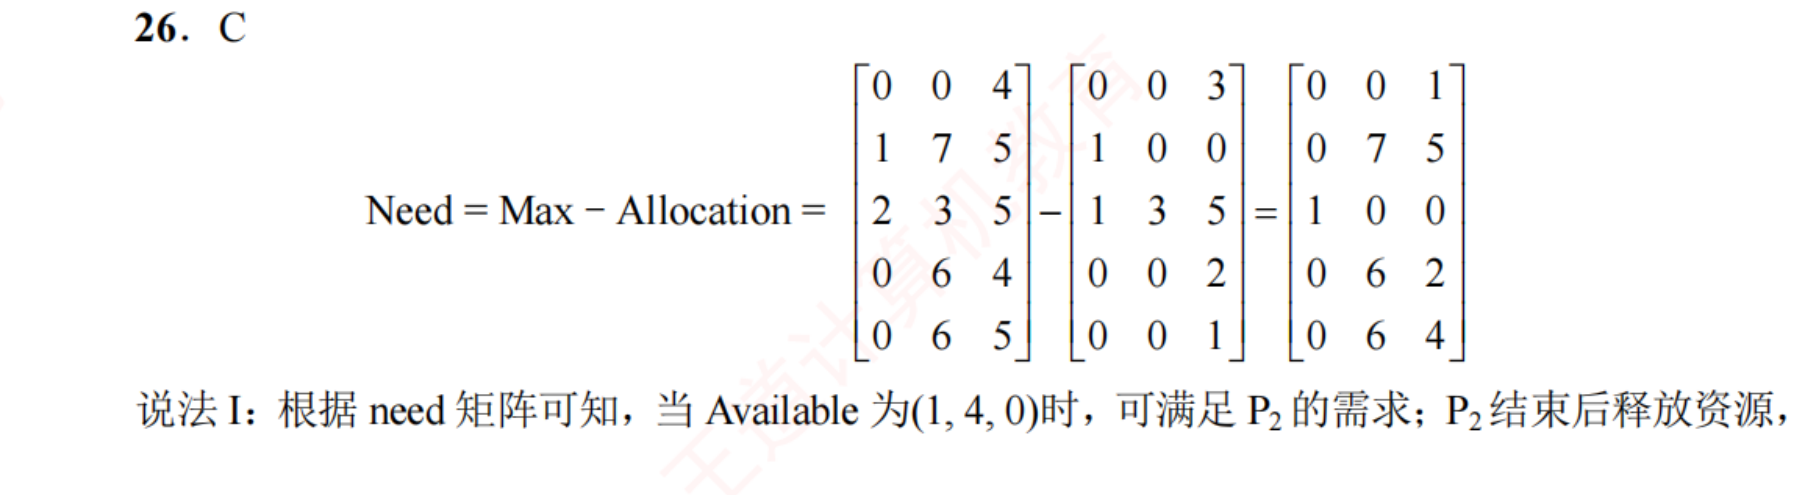
\includegraphics[width=161.13mm,height=180mm,keepaspectratio]{../solutions/assets/da8fe4d2b24e8c91c44ece6a.png}\par\smallskip
\par\medskip\noindent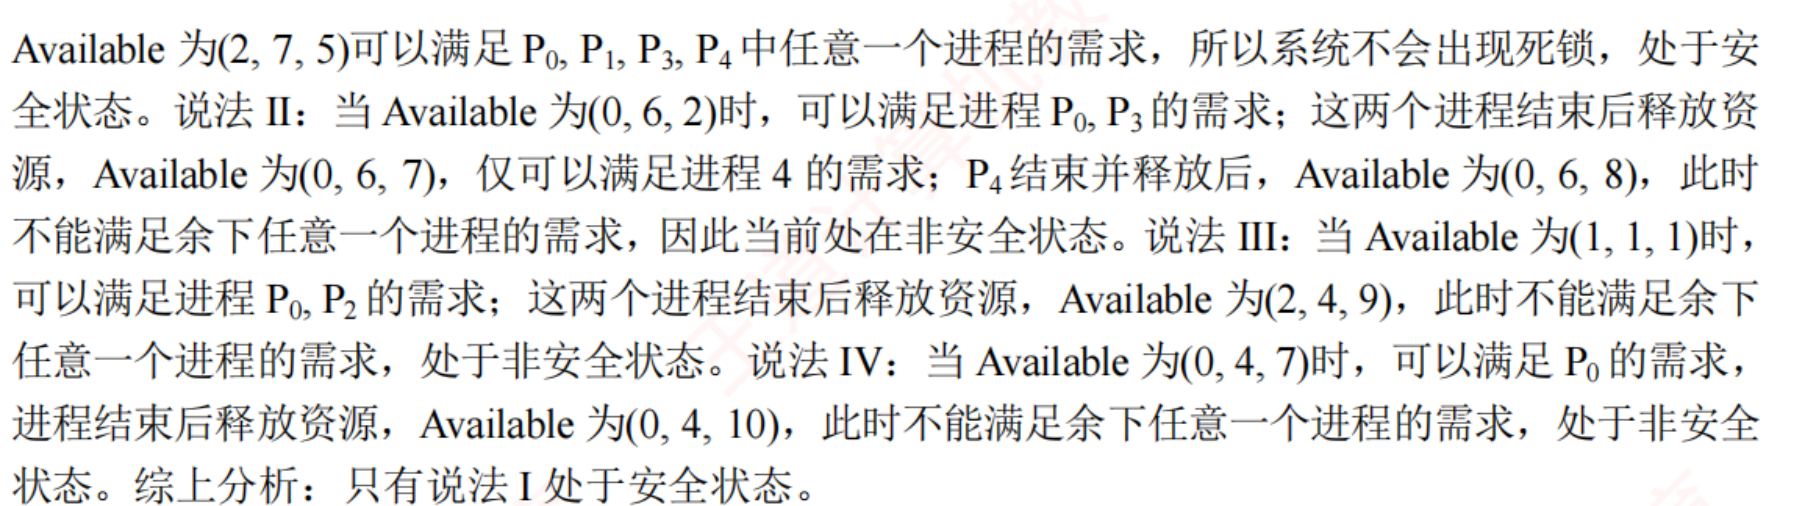
\includegraphics[width=161.13mm,height=180mm,keepaspectratio]{../solutions/assets/82bc39e34473ccdf641f57df.png}\par\smallskip
\section*{内存管理}
\par\medskip\Needspace{5\baselineskip}\noindent\hypertarget{a:OS03-E01}{}\label{a:OS03-E01}\textbf{例 3-1}\quad C
\par\smallskip
\par\medskip\noindent
\includegraphics[width=161.13mm,height=180mm,keepaspectratio]{../solutions/assets/67f3d0503d7fd8a9c22815ae.png}\par\smallskip
\par\medskip\noindent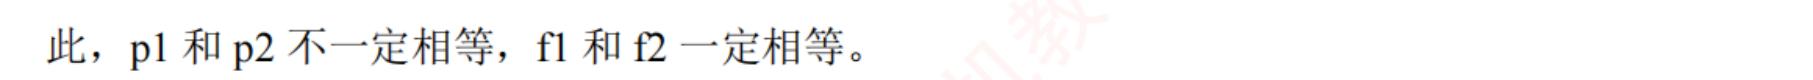
\includegraphics[width=161.13mm,height=180mm,keepaspectratio]{../solutions/assets/c49fa468f761b4b70c9e2b71.png}\par\smallskip
\par\medskip\Needspace{5\baselineskip}\noindent\hypertarget{a:OS03-E02}{}\label{a:OS03-E02}\textbf{例 3-2}\quad B；9 MB
\par\smallskip
\par\medskip\noindent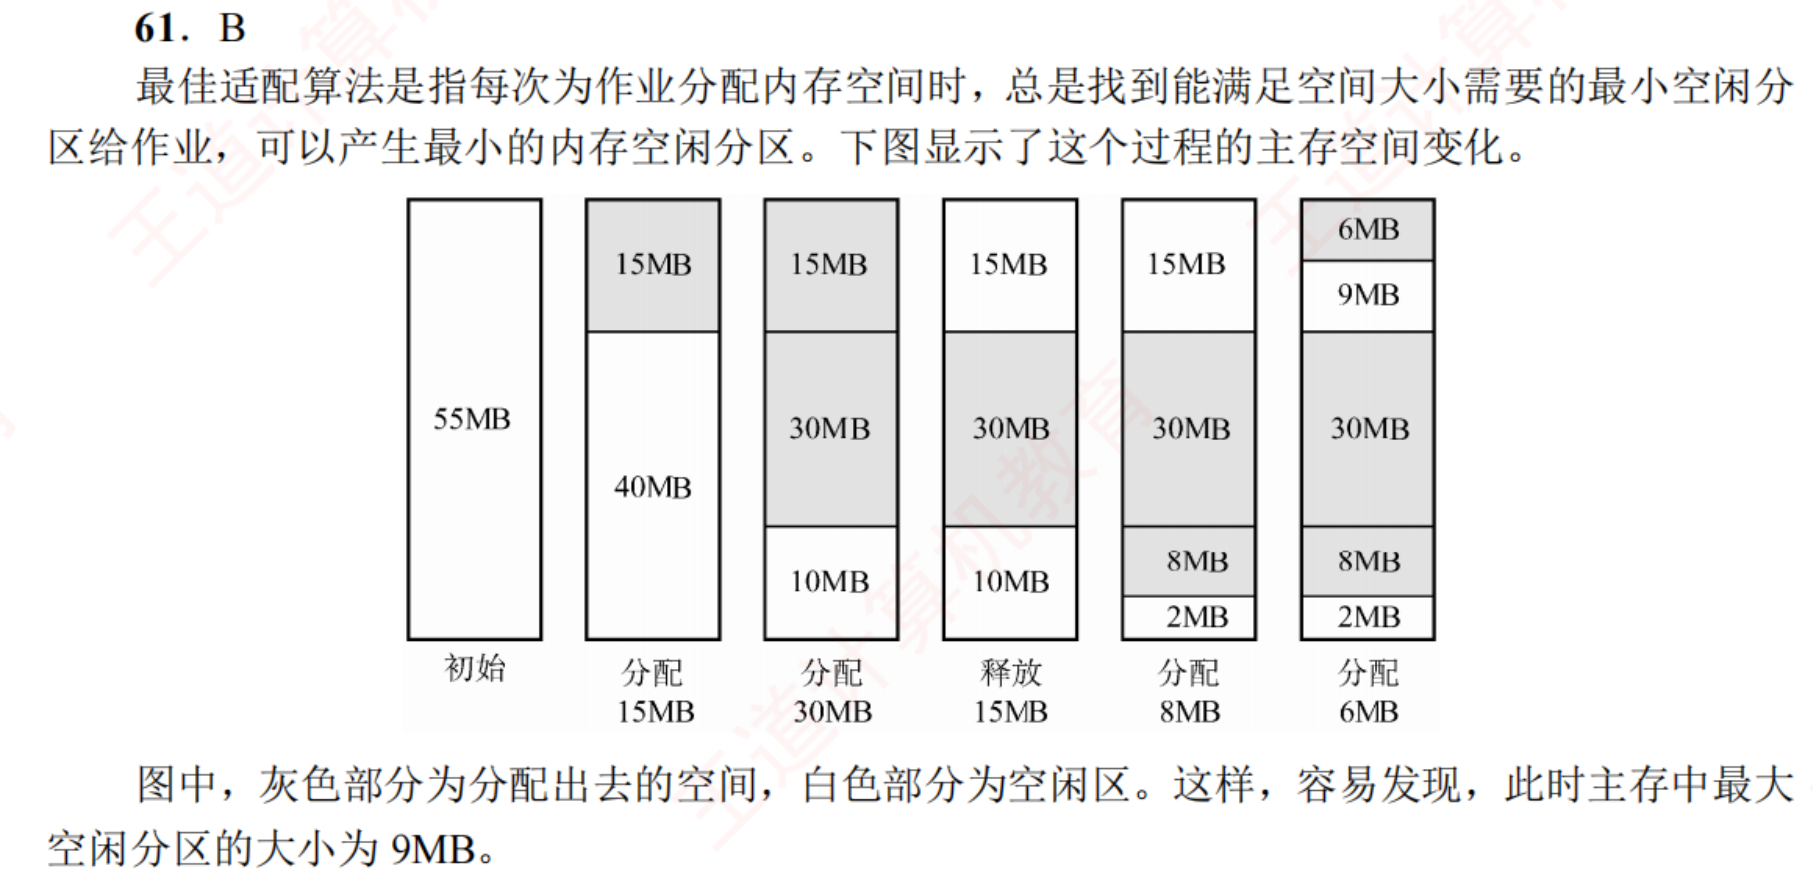
\includegraphics[width=161.13mm,height=180mm,keepaspectratio]{../solutions/assets/e8f98993ffe609ad29d459cc.png}\par\smallskip
\par\medskip\Needspace{5\baselineskip}\noindent\hypertarget{a:OS03-E03}{}\label{a:OS03-E03}\textbf{例 3-3}\quad B；128
\par\smallskip
按原解每张下级页表占一页，可放 \(2^{10}/2=2^9\) 项；覆盖 \(2^{16}\) 页需 \(2^{16}/2^9=2^7=128\) 个目录项。字段为7位目录、9位页号、10位偏移。该页表按页存放是原解采用的布局条件。

\par\medskip\Needspace{5\baselineskip}\noindent\hypertarget{a:OS03-E04}{}\label{a:OS03-E04}\textbf{例 3-4}\quad A；081H、101H
\par\smallskip
偏移为低12位225H；目录号 \(VA\gg22=081_H\)；下级页号 \((VA\gg12)\mathbin{\&}3FF_H=101_H\)。10位字段须按二进制位宽提取。

\par\medskip\Needspace{5\baselineskip}\noindent\hypertarget{a:OS03-E05}{}\label{a:OS03-E05}\textbf{例 3-5}\quad C；5次
\par\smallskip
按原解页框初始空，LRU 从最久到最近记录：

\begin{longtable}[]{@{}lll@{}}
\toprule\noalign{}
引用 & 更新后次序 & 结果 \\
\midrule\noalign{}
\endhead
\bottomrule\noalign{}
\endlastfoot
0、1、2、7 & 0、1、2、7 & 4次初装 \\
0 & 1、2、7、0 & 命中 \\
5 & 2、7、0、5 & 淘汰1 \\
3 & 7、0、5、3 & 淘汰2 \\
5 & 7、0、3、5 & 命中 \\
0 & 7、3、5、0 & 命中 \\
2 & 3、5、0、2 & 淘汰7 \\
7 & 5、0、2、7 & 淘汰3 \\
6 & 0、2、7、6 & 淘汰5 \\
\end{longtable}

9次缺页减4次空框装入，共5次置换。

\par\medskip\Needspace{5\baselineskip}\noindent\hypertarget{a:OS03-E06}{}\label{a:OS03-E06}\textbf{例 3-6}\quad C；60A01H
\par\smallskip
页号2、偏移A01H，存在位0，须调页。固定两框已满，页3、4的状态为 \((1,0)\)、\((1,1)\)，改进 Clock 清访问位后先选干净的页3。页2装入框60H，\(PA=60_H\times1000_H+A01_H=60A01_H\)；旧页框字段20H在存在位0时无效。

\par\medskip\Needspace{5\baselineskip}\noindent\hypertarget{a:OS03-E07}{}\label{a:OS03-E07}\textbf{例 3-7}\quad A；\{6,0,3,2\}
\par\smallskip
t 前最近六次引用为6、0、3、2、3、2，去重得到\{6,0,3,2\}。竖线右侧的0尚未访问。

\par\medskip\Needspace{5\baselineskip}\noindent\hypertarget{a:OS03-E08}{}\label{a:OS03-E08}\textbf{例 3-8}\quad 210 ns；100000220 ns；110 ns；101565H
\par\smallskip
\par\medskip\noindent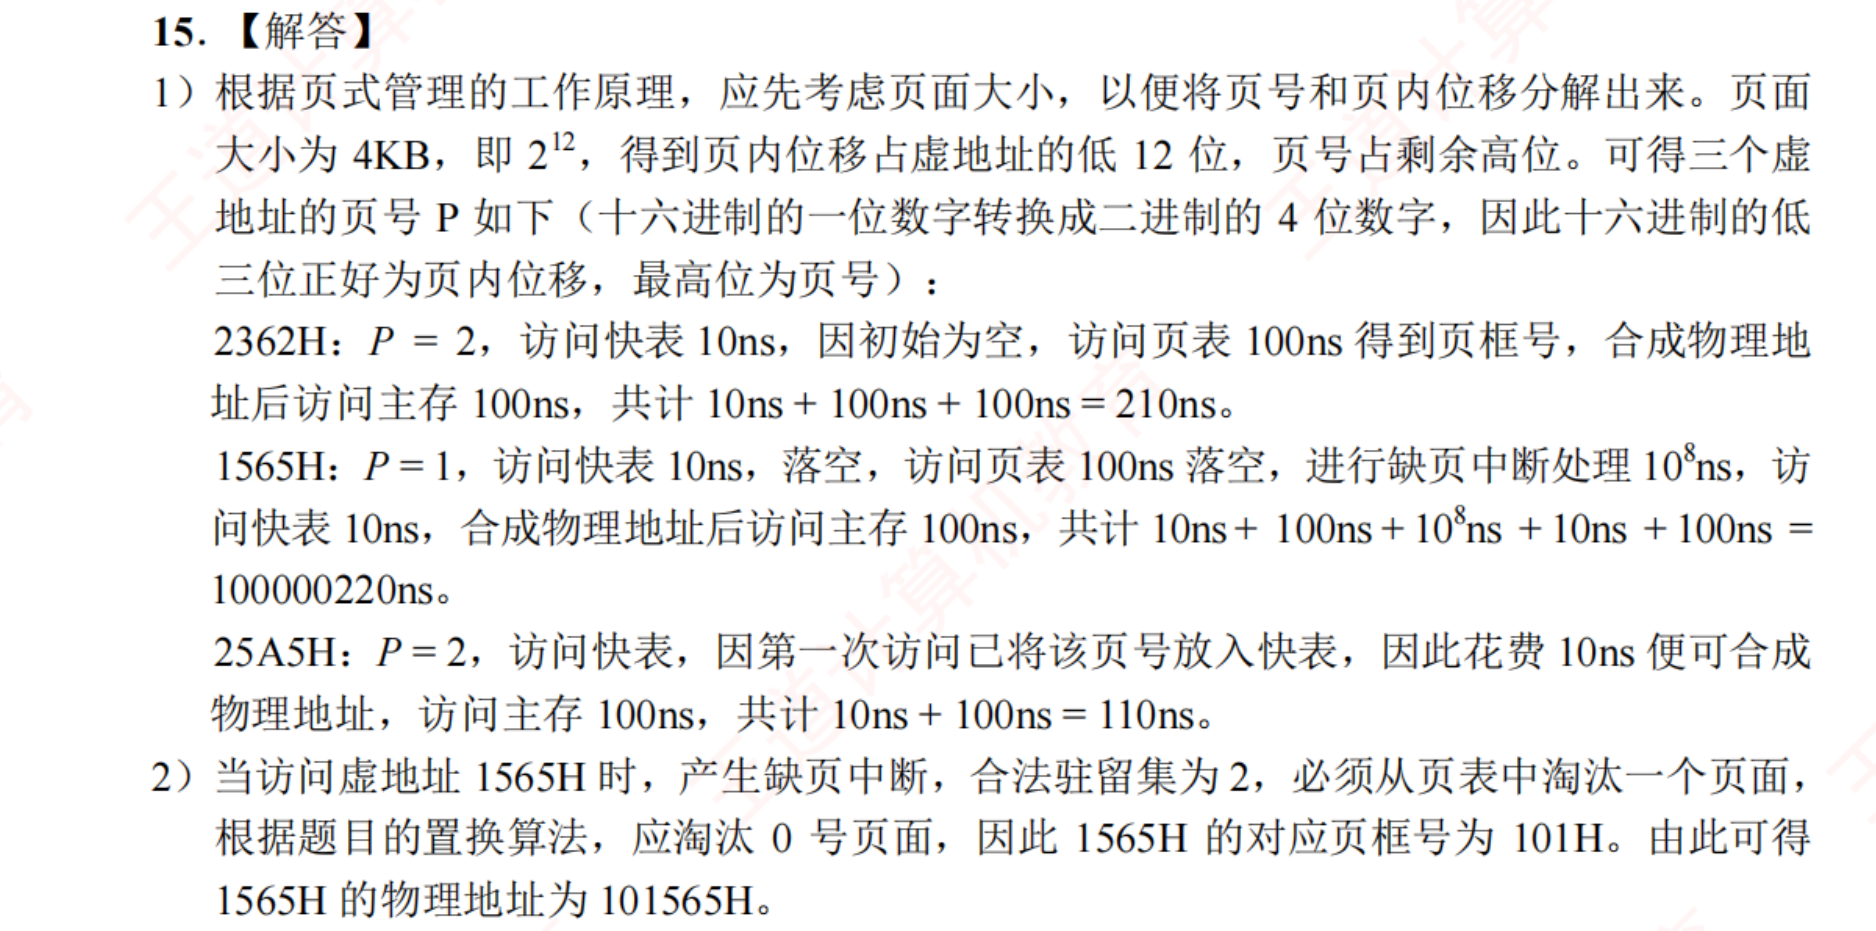
\includegraphics[width=162.00mm,height=180mm,keepaspectratio]{../solutions/assets/24195043a4868e19a82f4813.png}\par\smallskip
\par\medskip\Needspace{5\baselineskip}\noindent\hypertarget{a:OS03-E09}{}\label{a:OS03-E09}\textbf{例 3-9}\quad 10801008H；042H、001H；00201108H；00301004H
\par\smallskip
\par\medskip\noindent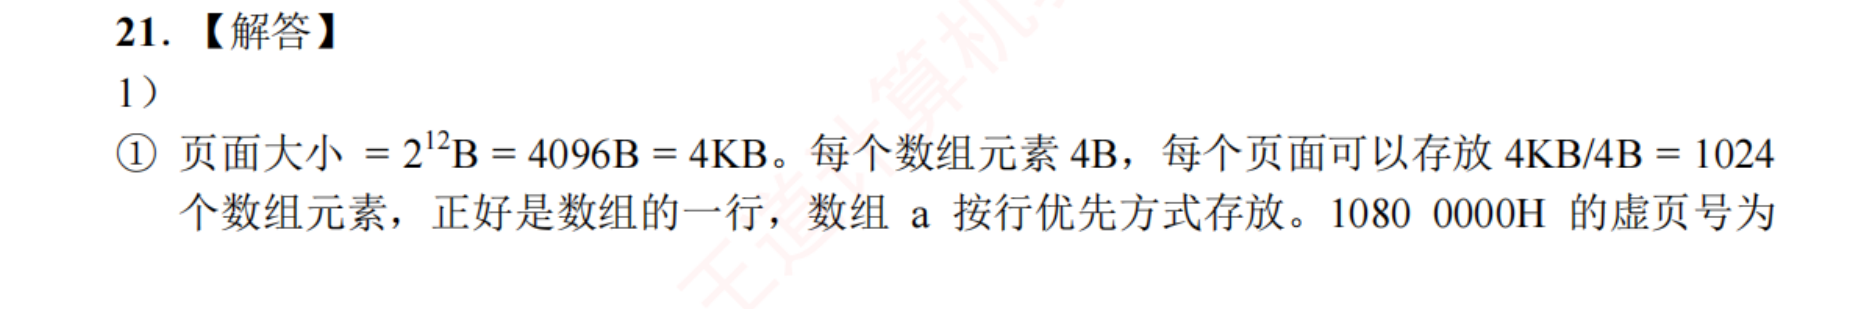
\includegraphics[width=162.00mm,height=180mm,keepaspectratio]{../solutions/assets/02b474afe6c4dff106e47baa.png}\par\smallskip
\par\medskip\noindent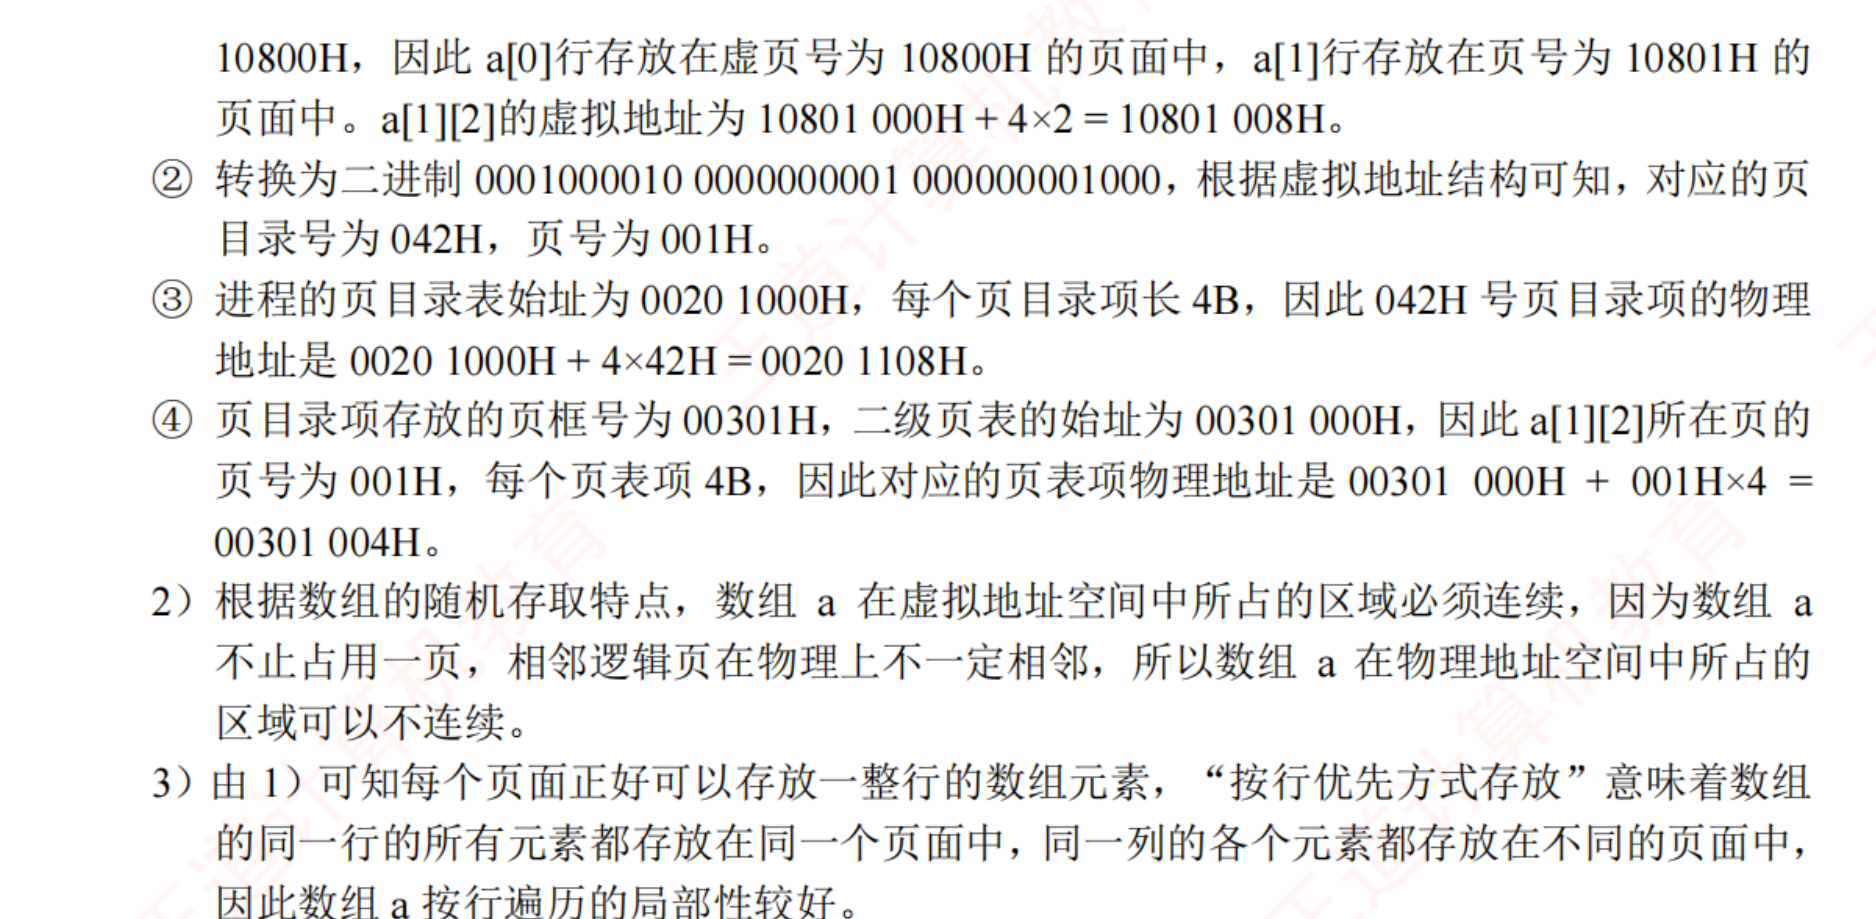
\includegraphics[width=162.00mm,height=180mm,keepaspectratio]{../solutions/assets/60d37cfd190c0ed53c367053.png}\par\smallskip
\section*{文件管理}
\par\medskip\Needspace{5\baselineskip}\noindent\hypertarget{a:OS04-E01}{}\label{a:OS04-E01}\textbf{例 4-1}\quad B
\par\smallskip
\par\medskip\noindent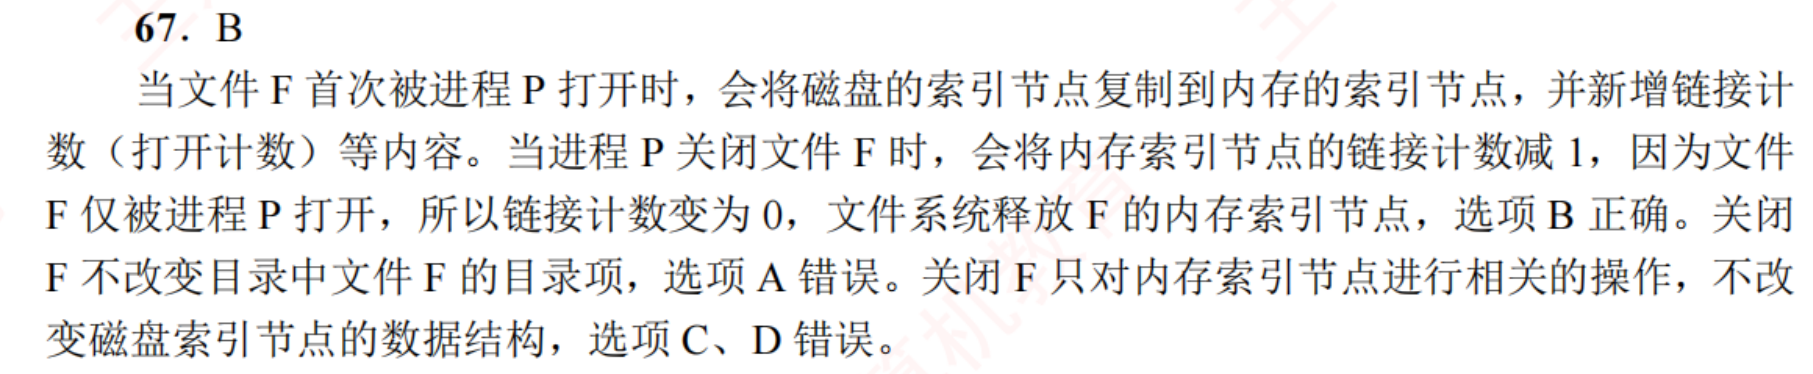
\includegraphics[width=161.13mm,height=180mm,keepaspectratio]{../solutions/assets/ccef49283e544b0ac61fa04a.png}\par\smallskip
\par\medskip\Needspace{5\baselineskip}\noindent\hypertarget{a:OS04-E02}{}\label{a:OS04-E02}\textbf{例 4-2}\quad D；20位
\par\smallskip
\par\medskip\noindent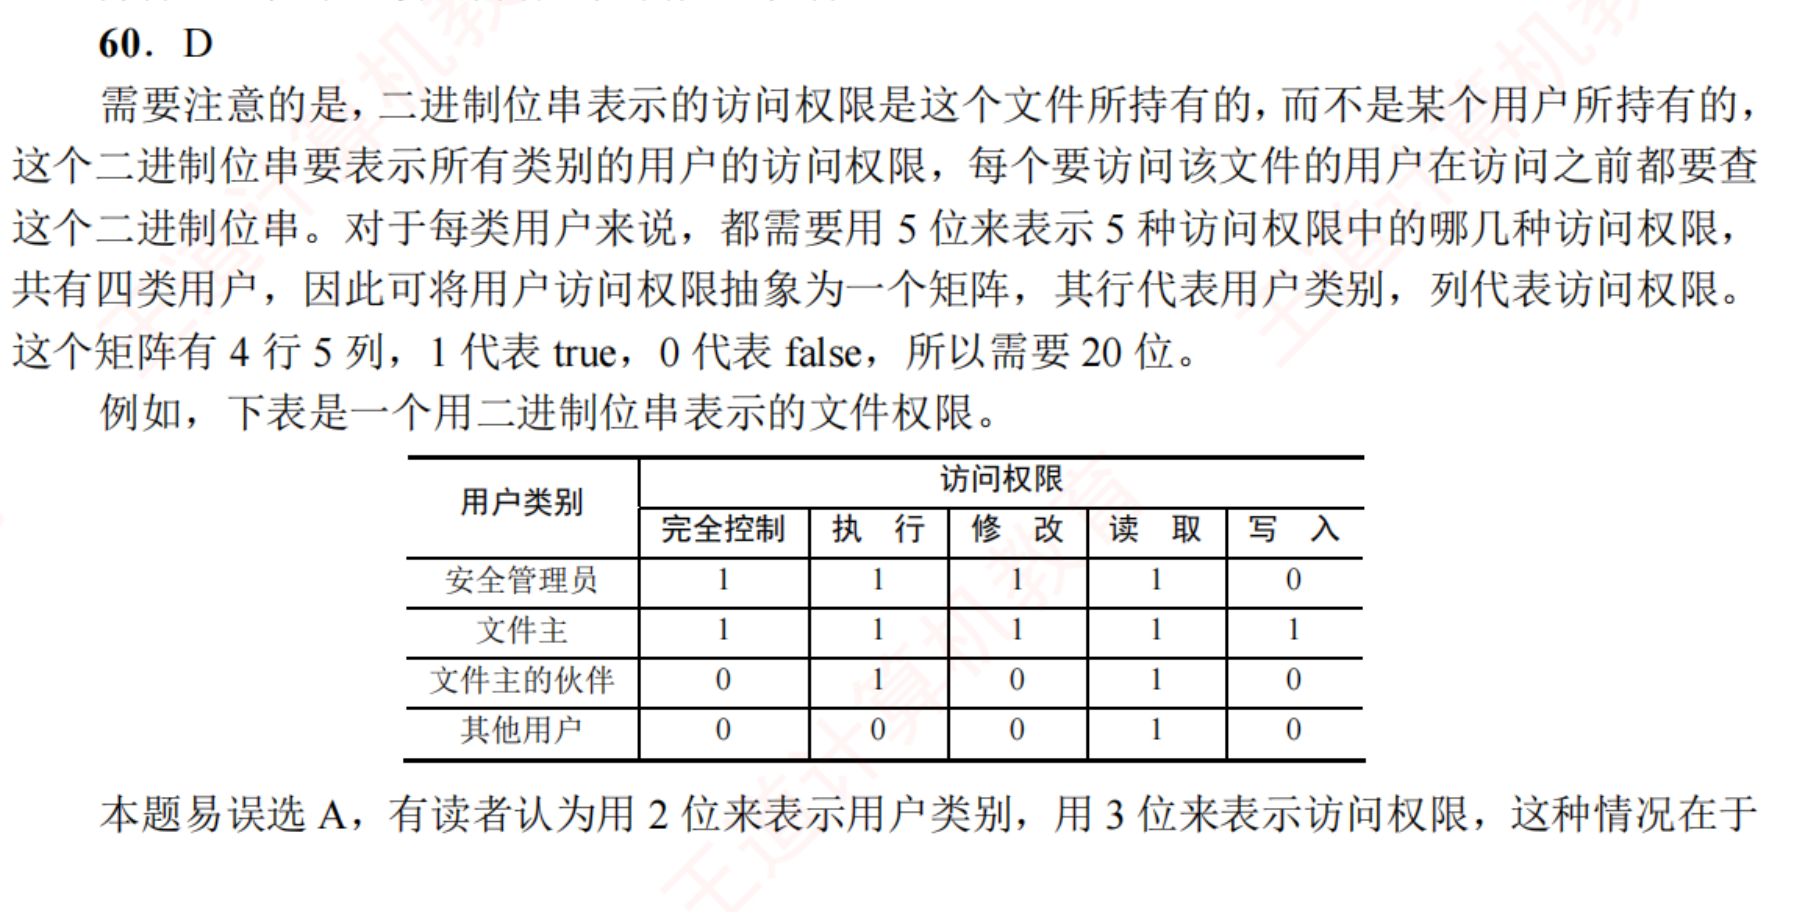
\includegraphics[width=161.13mm,height=180mm,keepaspectratio]{../solutions/assets/d36cfc7cd9dfd921f8c40fb0.png}\par\smallskip
\par\medskip\noindent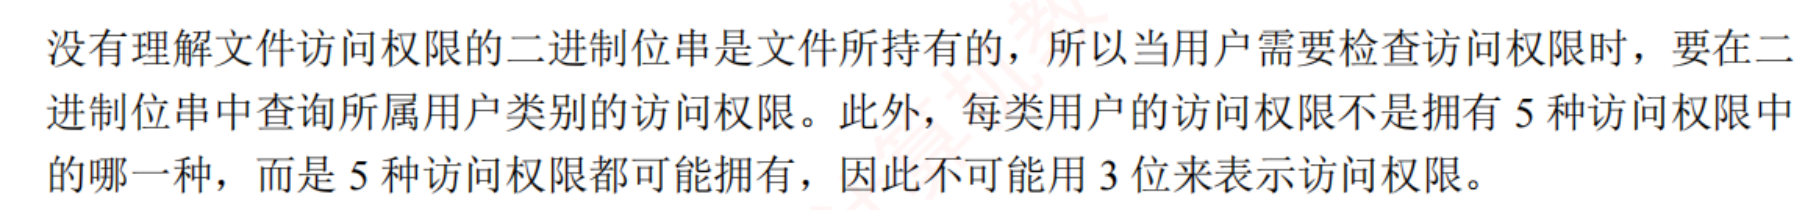
\includegraphics[width=161.13mm,height=180mm,keepaspectratio]{../solutions/assets/047fd8d4ee7e0c862d77cef1.png}\par\smallskip
\par\medskip\Needspace{5\baselineskip}\noindent\hypertarget{a:OS04-E03}{}\label{a:OS04-E03}\textbf{例 4-3}\quad B；1、3
\par\smallskip
\par\medskip\noindent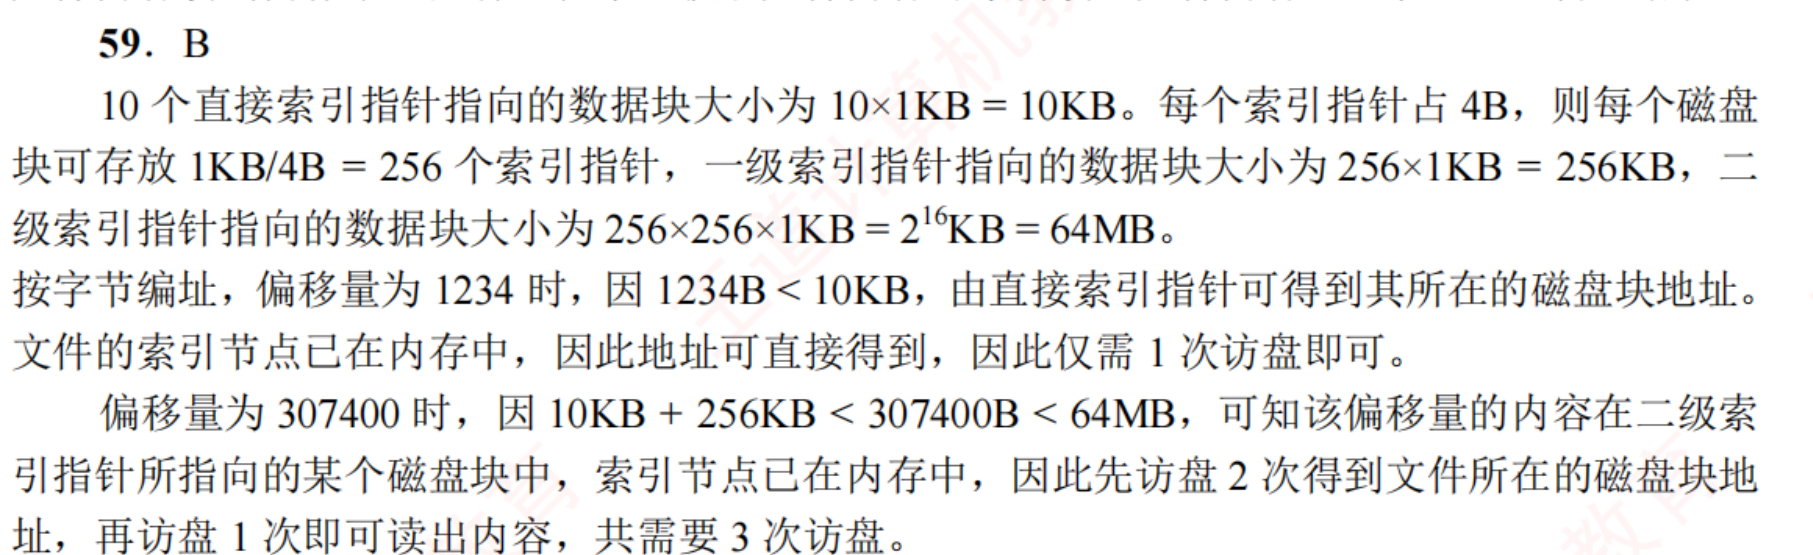
\includegraphics[width=161.13mm,height=180mm,keepaspectratio]{../solutions/assets/5f6c3271e21c9e30200a7ebb.png}\par\smallskip
\par\medskip\Needspace{5\baselineskip}\noindent\hypertarget{a:OS04-E04}{}\label{a:OS04-E04}\textbf{例 4-4}\quad D；6次
\par\smallskip
\par\medskip\noindent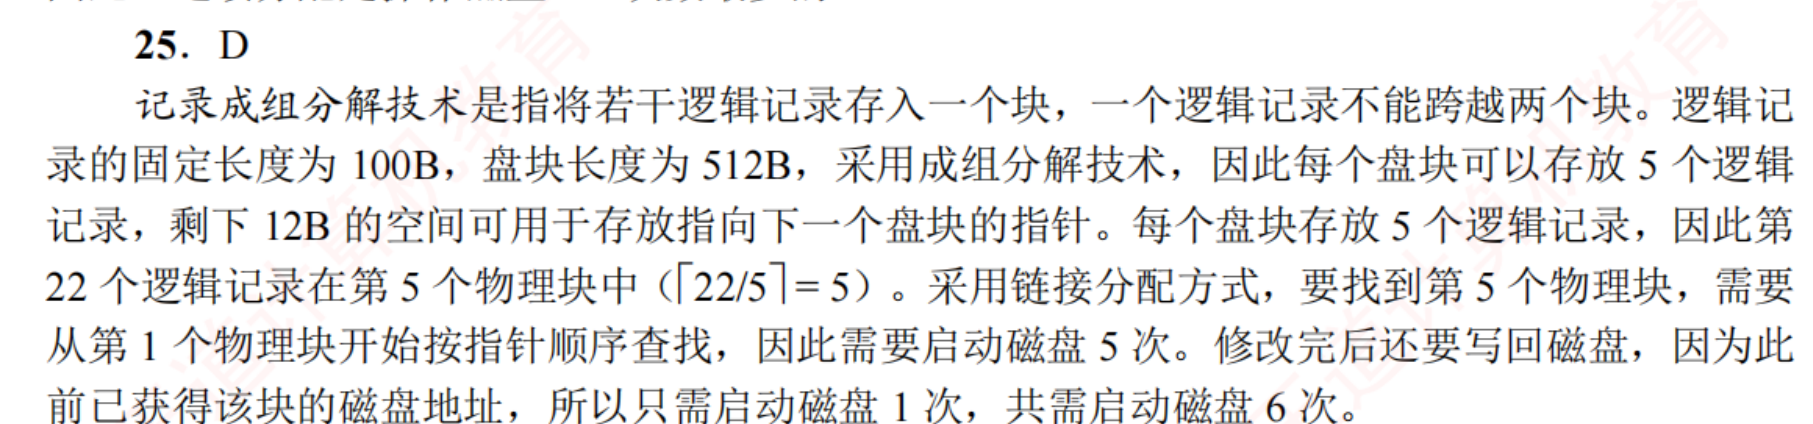
\includegraphics[width=161.13mm,height=180mm,keepaspectratio]{../solutions/assets/373b0c54ba10fb5d72f3920c.png}\par\smallskip
\par\medskip\Needspace{5\baselineskip}\noindent\hypertarget{a:OS04-E05}{}\label{a:OS04-E05}\textbf{例 4-5}\quad B
\par\smallskip
\par\medskip\noindent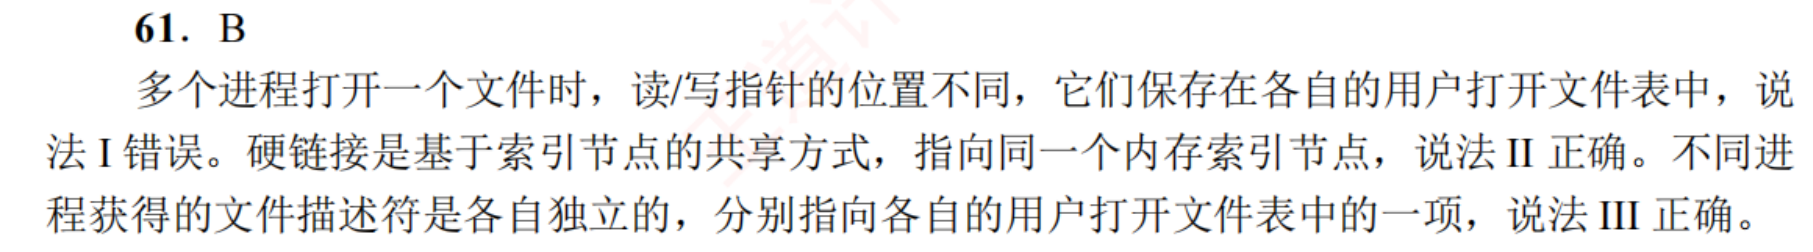
\includegraphics[width=161.13mm,height=180mm,keepaspectratio]{../solutions/assets/a21197c4a07183d3a8772f7d.png}\par\smallskip
\par\medskip\Needspace{5\baselineskip}\noindent\hypertarget{a:OS04-E06}{}\label{a:OS04-E06}\textbf{例 4-6}\quad C；82、1
\par\smallskip
\par\medskip\noindent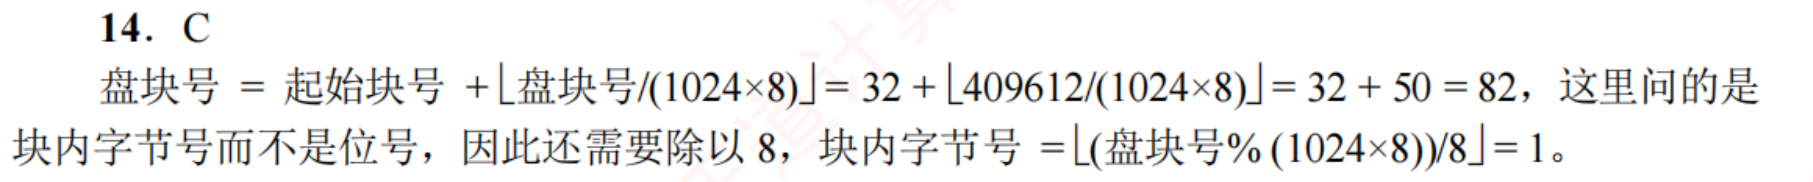
\includegraphics[width=161.13mm,height=180mm,keepaspectratio]{../solutions/assets/0ac09cbbf381a94f12038cf4.png}\par\smallskip
\par\medskip\Needspace{5\baselineskip}\noindent\hypertarget{a:OS04-E07}{}\label{a:OS04-E07}\textbf{例 4-7}\quad （course,2）、（doc,10）；30；2块；一级和二级
\par\smallskip
（1）stu 的两目录项为 \texttt{(course,2)}、\texttt{(doc,10)}，按图给定子项作答。

（2）doc 与 course1 同属该文件系统的 inode10，数据块号相同，x=30。

（3）course 目录内容已缓存，取得 inode号后还须读 inode 所在块、数据块30，共2块；题设未给这两者缓存。

（4）6 MiB 需1536个4 KiB数据块；每索引块1024项，直接及一级共1034块，还差502块，须用一级及二级间接，无需三级。一级区用1个索引块；二级区用1个上层及1个下层索引块，索引开销另计。

\par\medskip\Needspace{5\baselineskip}\noindent\hypertarget{a:OS04-E08}{}\label{a:OS04-E08}\textbf{例 4-8}\quad \((8+1024+1024^2+1024^3)4096\) B；\(2^{26}\) 个；时间不同
\par\smallskip
（1）每索引簇容纳1024个簇号，用户长度上限为 \((8+1024+1024^2+1024^3)\times4096\) B，不含索引簇。

（2）每 inode簇放64个 inode，inode 区共 \(2^{20}\times64=2^{26}\) 个。5600 B 图像各占2数据簇，数据区可放256M个，均在直接区无需间接簇；取较小值64M=\(67\,108\,864\)个，按题给可用区不另假设目录占用。

（3）F1末簇是逻辑簇1，在直接区；F2末簇是逻辑簇9，需一级间接。inode同已缓存、间接索引未缓存时，取簇号后者多读一次索引簇；若还读目标数据则分别1、2次读盘。

\section*{输入输出管理}
\par\medskip\Needspace{5\baselineskip}\noindent\hypertarget{a:OS05-E01}{}\label{a:OS05-E01}\textbf{例 5-1}\quad C
\par\smallskip
\par\medskip\noindent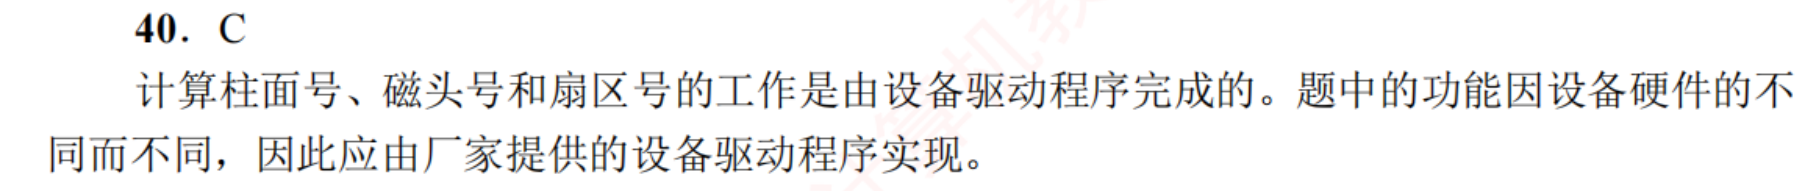
\includegraphics[width=161.13mm,height=180mm,keepaspectratio]{../solutions/assets/97876980c3100f8d0370d2db.png}\par\smallskip
\par\medskip\Needspace{5\baselineskip}\noindent\hypertarget{a:OS05-E02}{}\label{a:OS05-E02}\textbf{例 5-2}\quad B；1550 μs、1100 μs
\par\smallskip
\par\medskip\noindent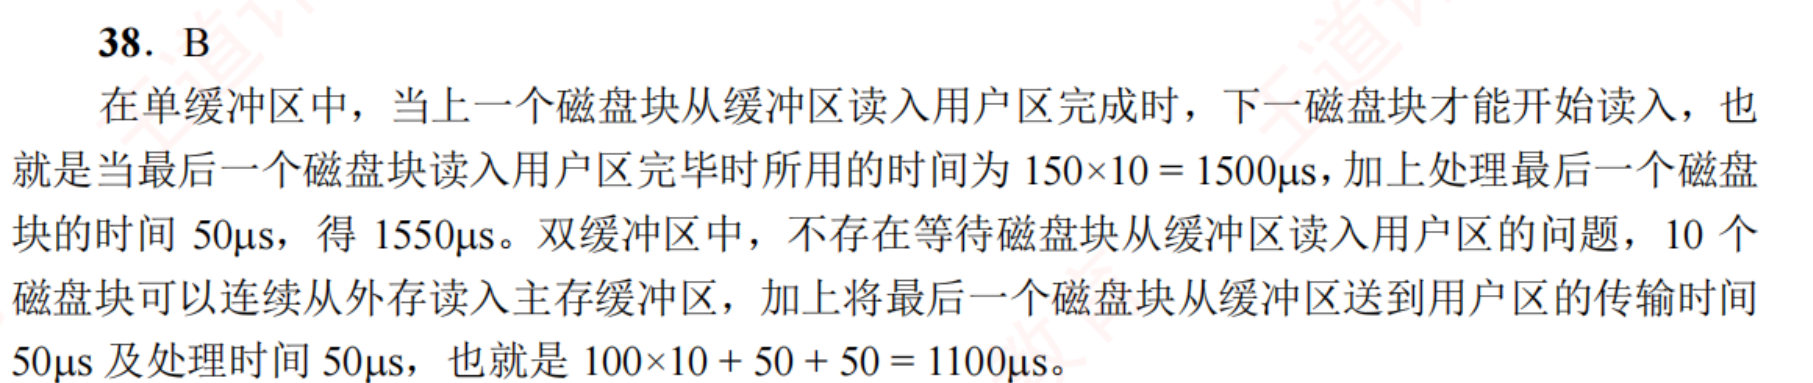
\includegraphics[width=161.13mm,height=180mm,keepaspectratio]{../solutions/assets/5a0c96e1c8f6ae9334dfad20.png}\par\smallskip
\par\medskip\Needspace{5\baselineskip}\noindent\hypertarget{a:OS05-E03}{}\label{a:OS05-E03}\textbf{例 5-3}\quad B；5046
\par\smallskip
\par\medskip\noindent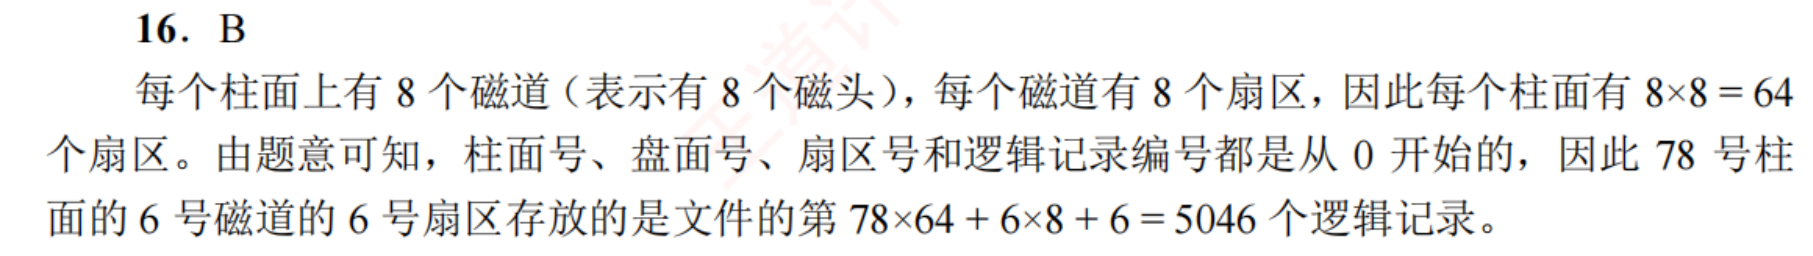
\includegraphics[width=161.13mm,height=180mm,keepaspectratio]{../solutions/assets/6883a25de39d6ea98a5e5688.png}\par\smallskip
\par\medskip\Needspace{5\baselineskip}\noindent\hypertarget{a:OS05-E04}{}\label{a:OS05-E04}\textbf{例 5-4}\quad B
\par\smallskip
\par\medskip\noindent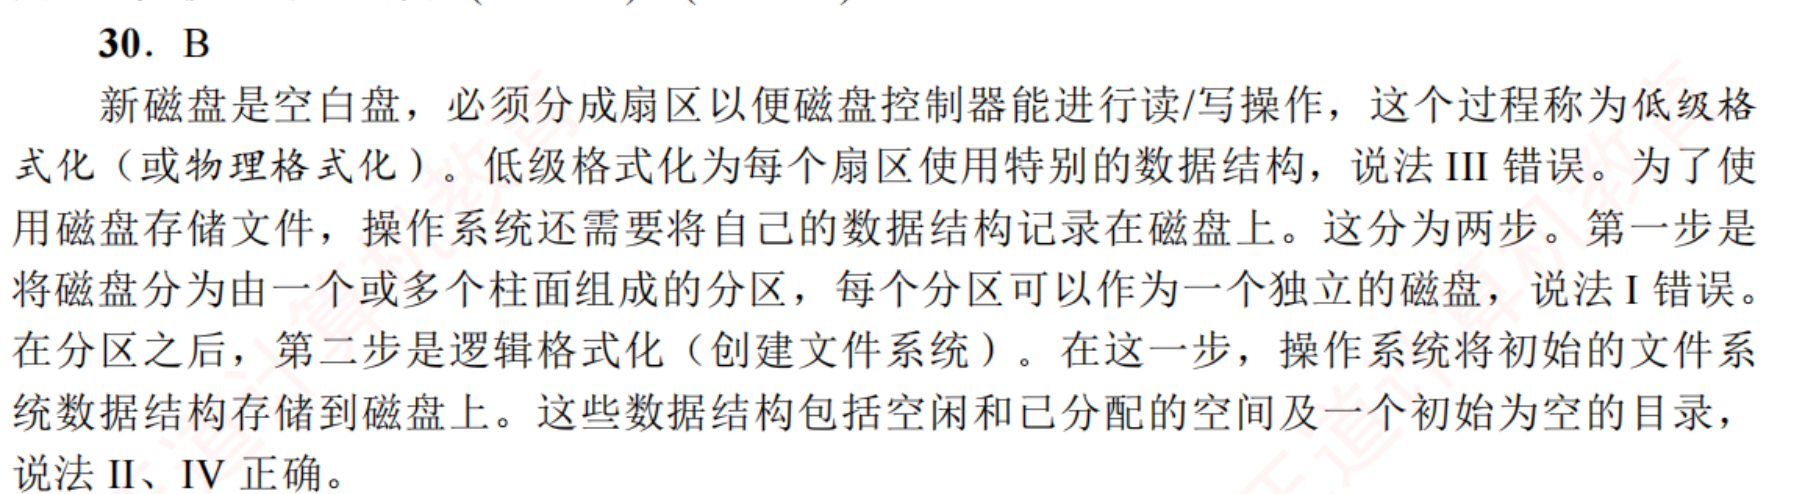
\includegraphics[width=161.13mm,height=180mm,keepaspectratio]{../solutions/assets/f3cac0928f1dc6ae0e24d7ef.png}\par\smallskip
\par\medskip\Needspace{5\baselineskip}\noindent\hypertarget{a:OS05-E05}{}\label{a:OS05-E05}\textbf{例 5-5}\quad C；325
\par\smallskip
\par\medskip\noindent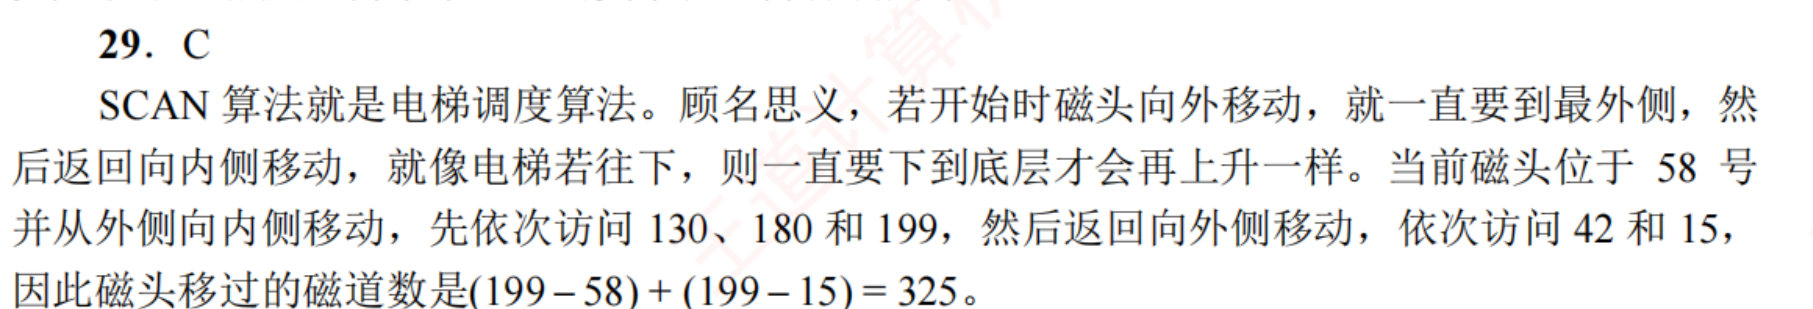
\includegraphics[width=161.13mm,height=180mm,keepaspectratio]{../solutions/assets/b63761c895484ff1b224b0e2.png}\par\smallskip
\par\medskip\Needspace{5\baselineskip}\noindent\hypertarget{a:OS05-E06}{}\label{a:OS05-E06}\textbf{例 5-6}\quad ②→⑥→④→③→①→⑤；③为驱动；处理入口时P阻塞、CPU内核态
\par\smallskip
六项次序为②\ensuremath{\to}⑥\ensuremath{\to}④\ensuremath{\to}③\ensuremath{\to}①\ensuremath{\to}⑤：P 无字符可读先阻塞，键入后中断入口启动，驱动读字符至系统缓冲，唤醒 P，P 被调度后返回系统调用。

（1）①前③、后⑤，⑥后④，仅比较题列操作。（2）②后当前 P 必须让出 CPU，无其他就绪者时进 idle；①后 P 恢复可调度资格。（3）③执行具体控制器读入，属于驱动。（4）入口及读字符阶段 P 仍阻塞，执行①才就绪；CPU 执行中断处理在内核态，被中断者可能为另一进程。

\par\medskip\Needspace{5\baselineskip}\noindent\hypertarget{a:OS05-E07}{}\label{a:OS05-E07}\textbf{例 5-7}\quad 307200000 B；100260→101660→110560→60005；（100,5,60）；驱动
\par\smallskip
（1）容量 \(300\times10\times200\times512=307200000\) B，即300000 KiB。每簇1024 B，每柱面1000簇。

（2）请求柱面依次为100、60、101、110。SSTF 从85先到100，再到101、110、60，对应簇100260、101660、110560、60005；距离分别15、1、9、50，共75柱面。每步按新磁头位置重算。

（3）\(100530=100\times1000+530\)，\(530=5\times100+30\)，故柱面100、磁头5，磁道内第30簇从扇区60开始并含61。起始 CHS 为（100,5,60），各字段0基。按本题传统几何模型由磁盘驱动转换。

\chapter{计算机网络}
\section*{计算机网络体系结构}
\par\medskip\Needspace{5\baselineskip}\noindent\hypertarget{a:CN01-E01}{}\label{a:CN01-E01}\textbf{例 1-1}\quad B
\par\smallskip
\par\medskip\noindent
\includegraphics[width=161.13mm,height=180mm,keepaspectratio]{../solutions/assets/5f1653b5268052ff1f091c1b.png}\par\smallskip
\par\medskip\Needspace{5\baselineskip}\noindent\hypertarget{a:CN01-E02}{}\label{a:CN01-E02}\textbf{例 1-2}\quad B
\par\smallskip
\par\medskip\noindent
\includegraphics[width=161.13mm,height=180mm,keepaspectratio]{../solutions/assets/5a9910c9c08b9b94976283f3.png}\par\smallskip
\par\medskip\Needspace{5\baselineskip}\noindent\hypertarget{a:CN01-E03}{}\label{a:CN01-E03}\textbf{例 1-3}\quad D（80.10 ms）
\par\smallskip
按题设分组长度直接切分文件，分组数为 \(10^6/1000=1000\)，每组发送时间为 \(8000/10^8=80\ \mu s\)。每段传播时间由时延带宽积求得 \(1000/10^8=10\ \mu s\)。

两段链路上第一组用 \(2\times80+2\times10=180\ \mu s\) 到齐；后续999组每隔80 μs到齐。总计

\[180+999\times80=80100\ \mu s=80.10\text{ ms},\]

故选 \textbf{D}。本题按给定1000 B分组切分，不另添加未给定首部。

\par\medskip\Needspace{5\baselineskip}\noindent\hypertarget{a:CN01-E04}{}\label{a:CN01-E04}\textbf{例 1-4}\quad B
\par\smallskip
\par\medskip\noindent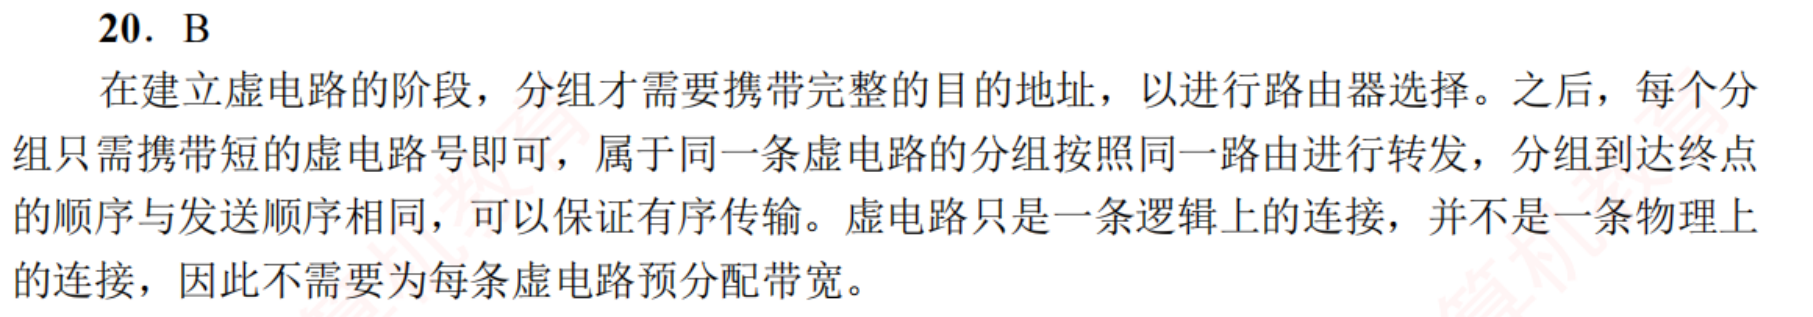
\includegraphics[width=161.13mm,height=180mm,keepaspectratio]{../solutions/assets/a27dc905a7524c7008e7a92b.png}\par\smallskip
\section*{物理层}
\par\medskip\Needspace{5\baselineskip}\noindent\hypertarget{a:CN02-E01}{}\label{a:CN02-E01}\textbf{例 2-1}\quad C
\par\smallskip
\par\medskip\noindent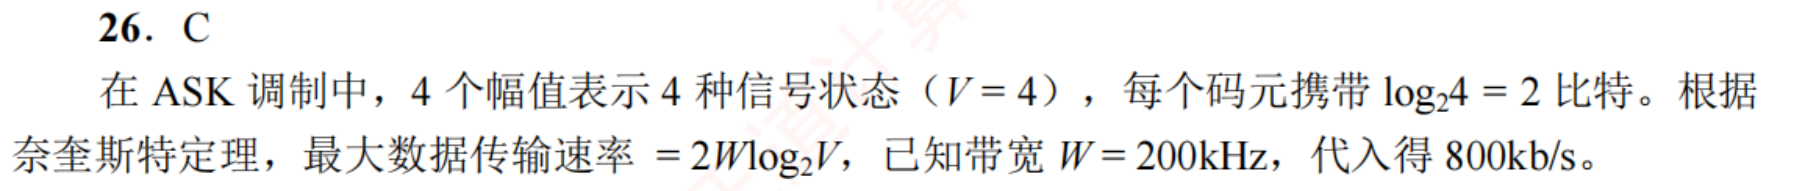
\includegraphics[width=161.13mm,height=180mm,keepaspectratio]{../solutions/assets/d26b27af76d981773fcff849.png}\par\smallskip
\par\medskip\Needspace{5\baselineskip}\noindent\hypertarget{a:CN02-E02}{}\label{a:CN02-E02}\textbf{例 2-2}\quad A（约2倍）
\par\smallskip
\par\medskip\noindent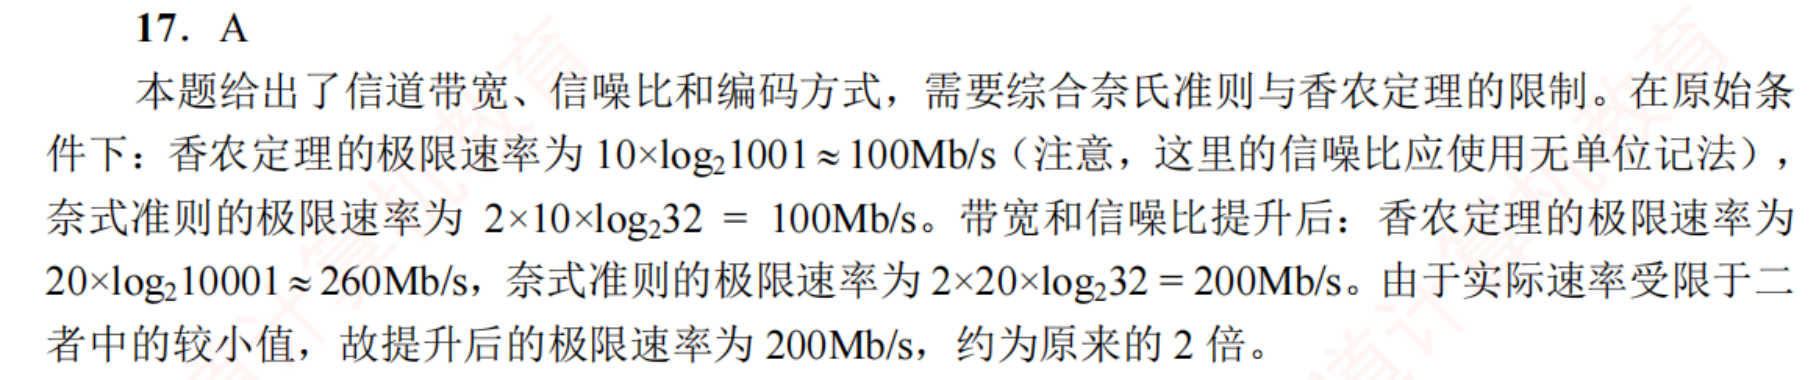
\includegraphics[width=161.13mm,height=180mm,keepaspectratio]{../solutions/assets/3b298a620167467c568c078e.png}\par\smallskip
\par\medskip\Needspace{5\baselineskip}\noindent\hypertarget{a:CN02-E03}{}\label{a:CN02-E03}\textbf{例 2-3}\quad C
\par\smallskip
\par\medskip\noindent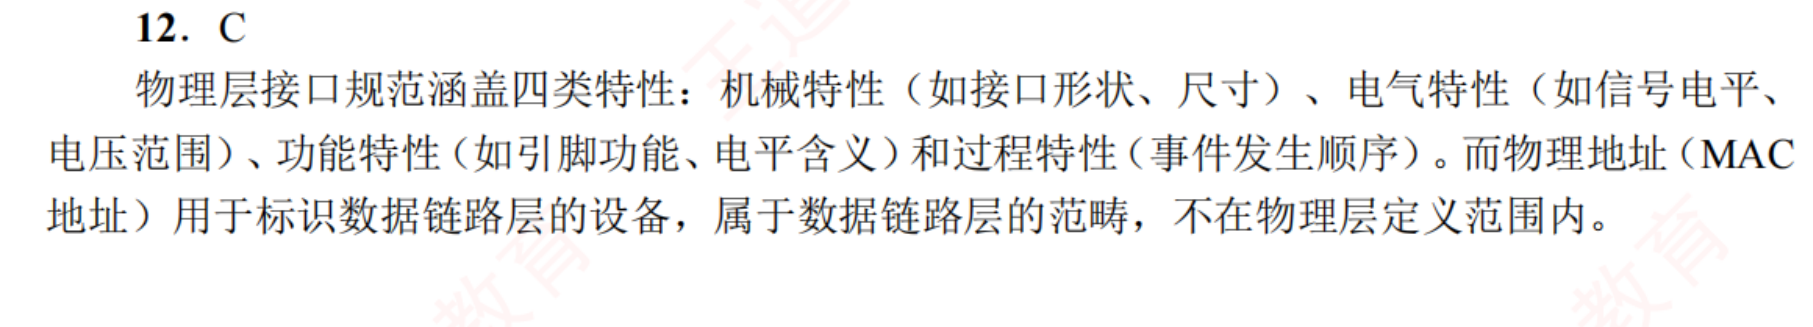
\includegraphics[width=161.13mm,height=180mm,keepaspectratio]{../solutions/assets/fcbefdcd023b0fa2d7640e06.png}\par\smallskip
\section*{数据链路层}
\par\medskip\Needspace{5\baselineskip}\noindent\hypertarget{a:CN03-E01}{}\label{a:CN03-E01}\textbf{例 3-1}\quad A
\par\smallskip
\par\medskip\noindent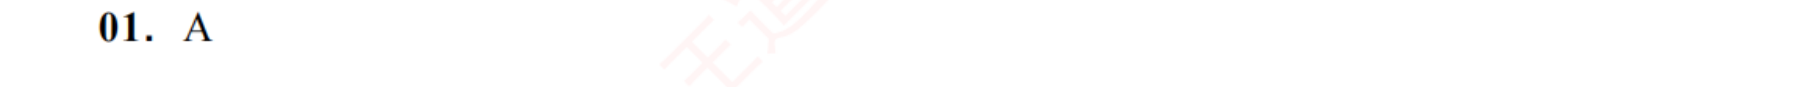
\includegraphics[width=161.13mm,height=180mm,keepaspectratio]{../solutions/assets/4ccebf17ff289f1f8ede7e6d.png}\par\smallskip
\par\medskip\noindent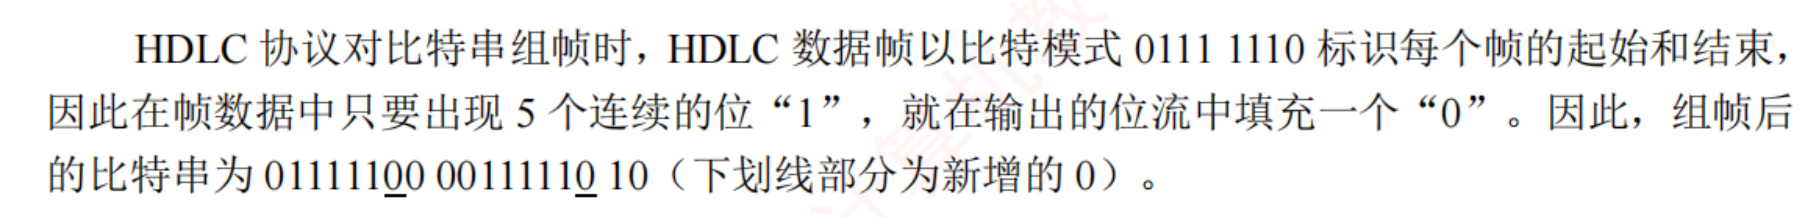
\includegraphics[width=161.13mm,height=180mm,keepaspectratio]{../solutions/assets/e9cec0190119c3ae2b2303c8.png}\par\smallskip
\par\medskip\Needspace{5\baselineskip}\noindent\hypertarget{a:CN03-E02}{}\label{a:CN03-E02}\textbf{例 3-2}\quad D
\par\smallskip
\par\medskip\noindent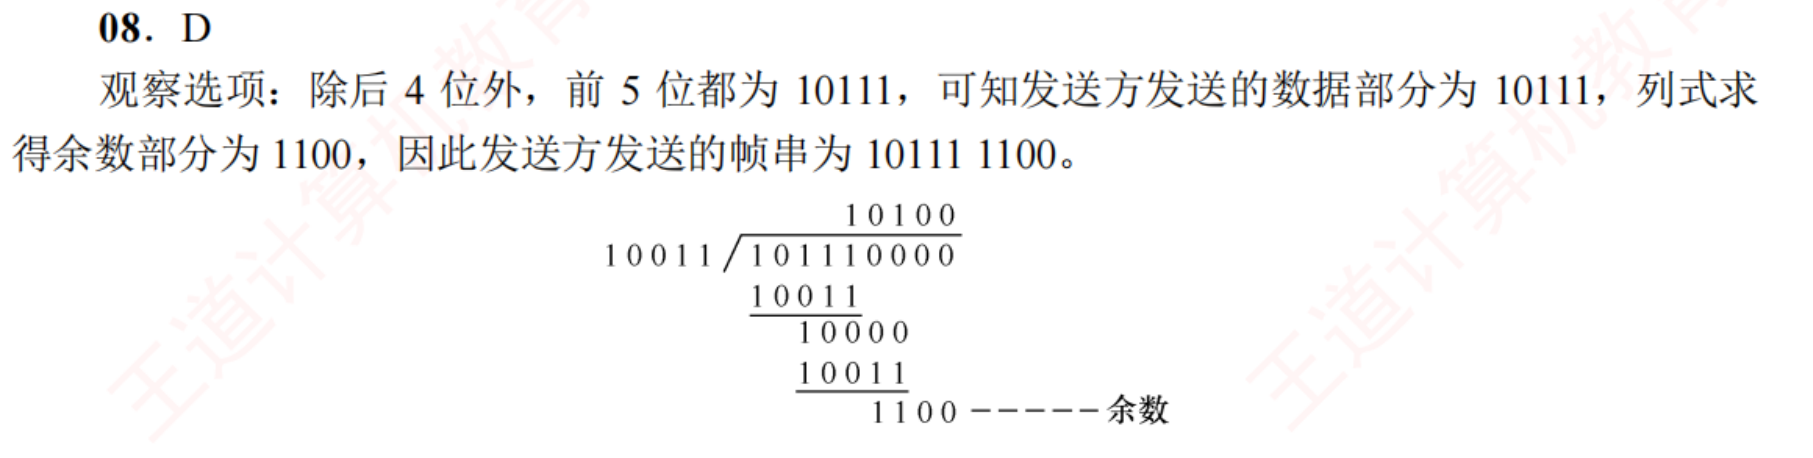
\includegraphics[width=161.13mm,height=180mm,keepaspectratio]{../solutions/assets/d1d490d24fe66c8525ab7809.png}\par\smallskip
\par\medskip\Needspace{5\baselineskip}\noindent\hypertarget{a:CN03-E03}{}\label{a:CN03-E03}\textbf{例 3-3}\quad C
\par\smallskip
\par\medskip\noindent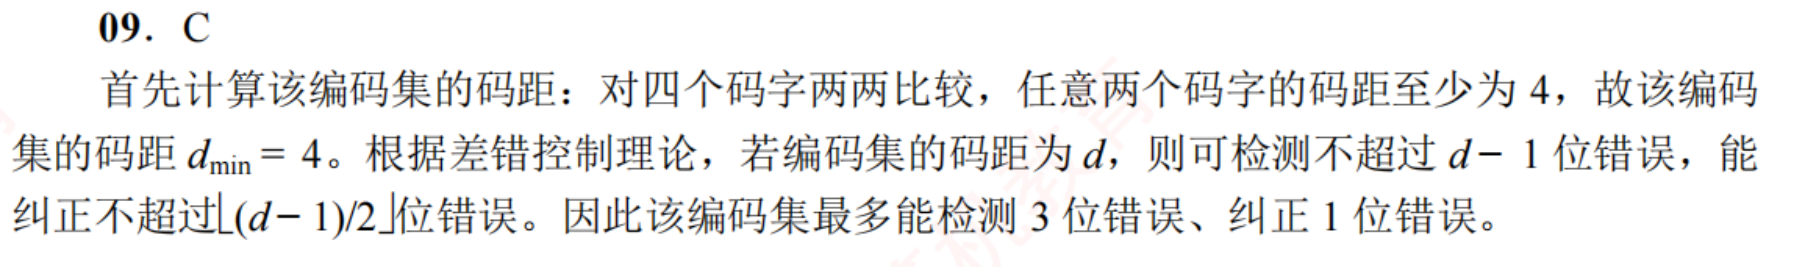
\includegraphics[width=161.13mm,height=180mm,keepaspectratio]{../solutions/assets/442db731578ebd6bd63ede06.png}\par\smallskip
\par\medskip\Needspace{5\baselineskip}\noindent\hypertarget{a:CN03-E04}{}\label{a:CN03-E04}\textbf{例 3-4}\quad D
\par\smallskip
\par\medskip\noindent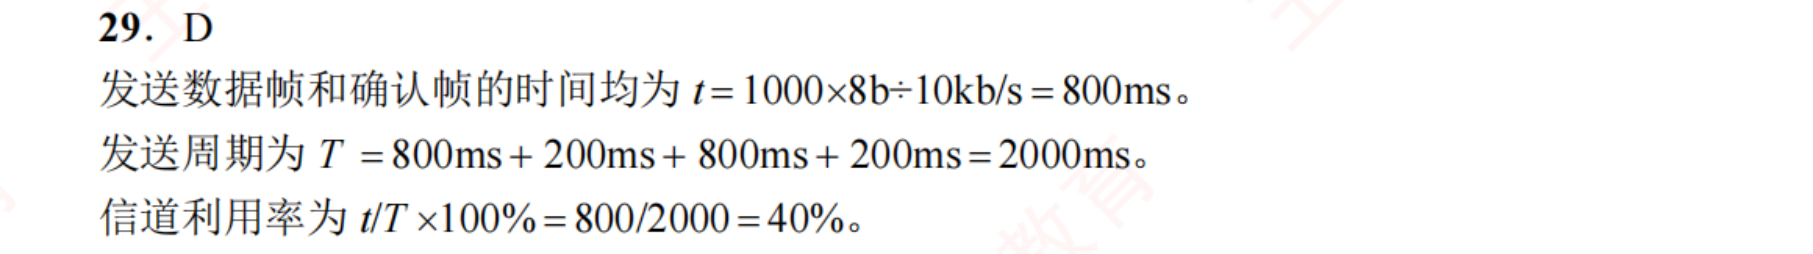
\includegraphics[width=161.13mm,height=180mm,keepaspectratio]{../solutions/assets/c769a2d8aabb6f49d16001f3.png}\par\smallskip
\par\medskip\Needspace{5\baselineskip}\noindent\hypertarget{a:CN03-E05}{}\label{a:CN03-E05}\textbf{例 3-5}\quad C
\par\smallskip
\par\medskip\noindent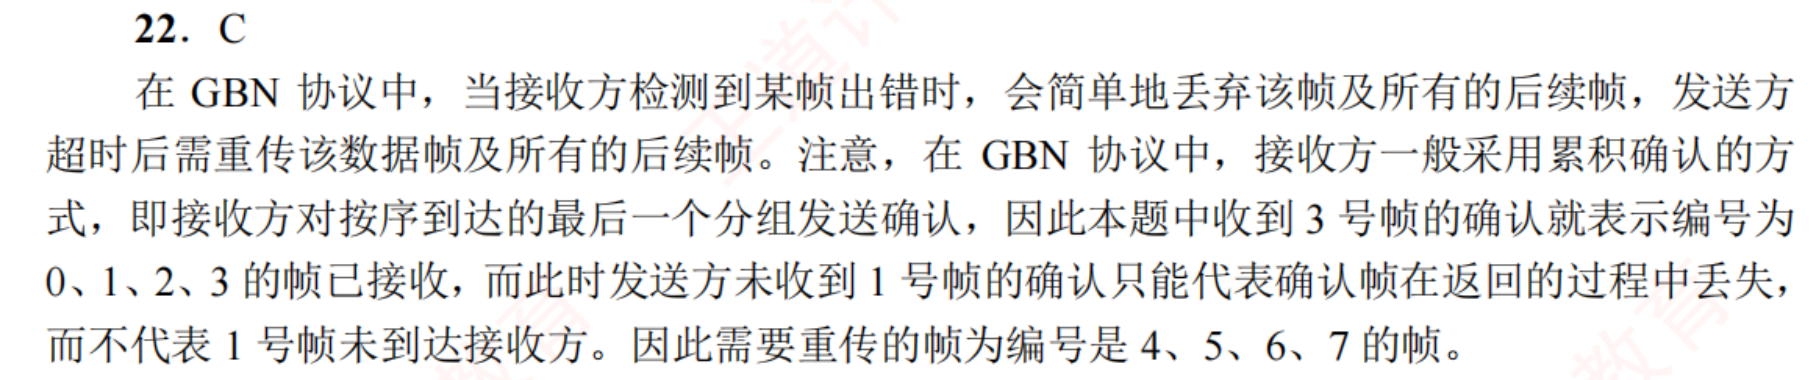
\includegraphics[width=161.13mm,height=180mm,keepaspectratio]{../solutions/assets/c986e6d4bb143e749e96466a.png}\par\smallskip
\par\medskip\Needspace{5\baselineskip}\noindent\hypertarget{a:CN03-E06}{}\label{a:CN03-E06}\textbf{例 3-6}\quad C
\par\smallskip
\par\medskip\noindent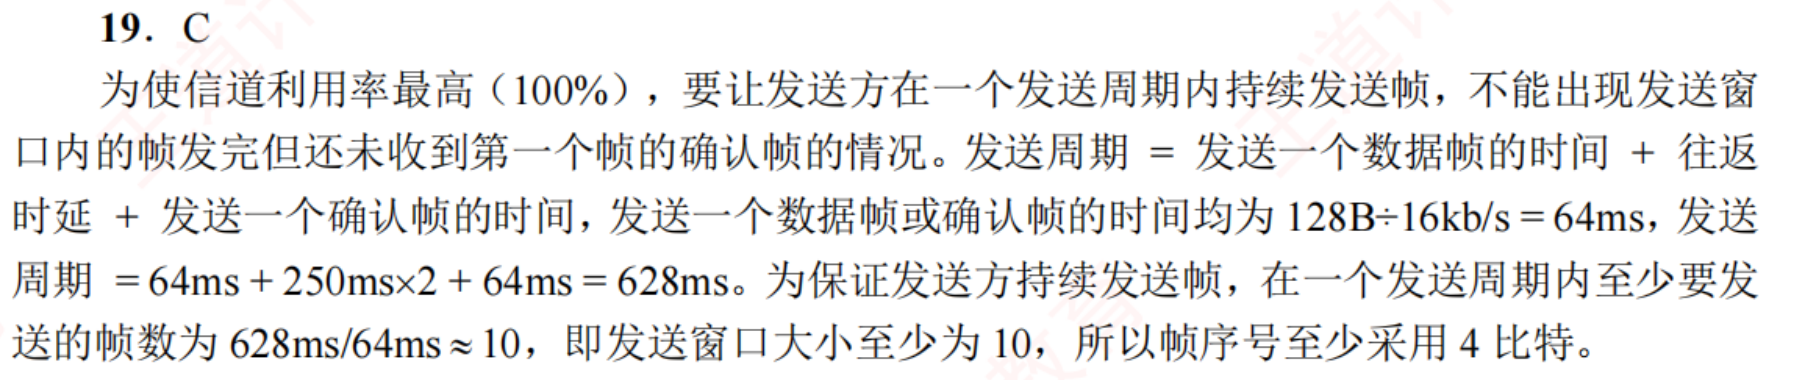
\includegraphics[width=161.13mm,height=180mm,keepaspectratio]{../solutions/assets/323c6efd6aa373655075092f.png}\par\smallskip
\par\medskip\Needspace{5\baselineskip}\noindent\hypertarget{a:CN03-E07}{}\label{a:CN03-E07}\textbf{例 3-7}\quad B
\par\smallskip
\par\medskip\noindent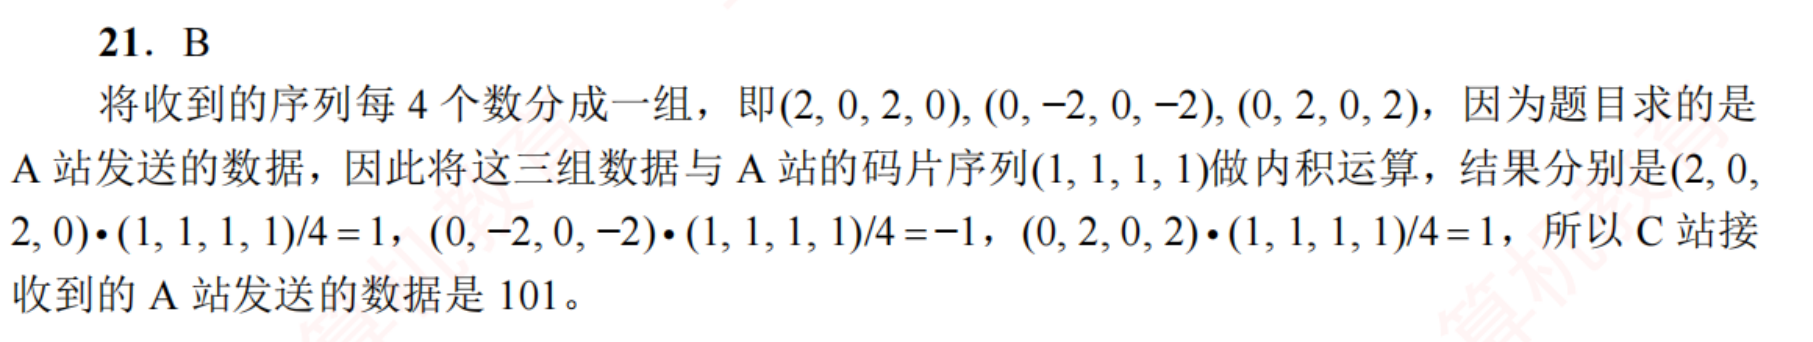
\includegraphics[width=161.13mm,height=180mm,keepaspectratio]{../solutions/assets/169c273babe5f90bd9c5ffb1.png}\par\smallskip
\par\medskip\Needspace{5\baselineskip}\noindent\hypertarget{a:CN03-E08}{}\label{a:CN03-E08}\textbf{例 3-8}\quad D
\par\smallskip
\par\medskip\noindent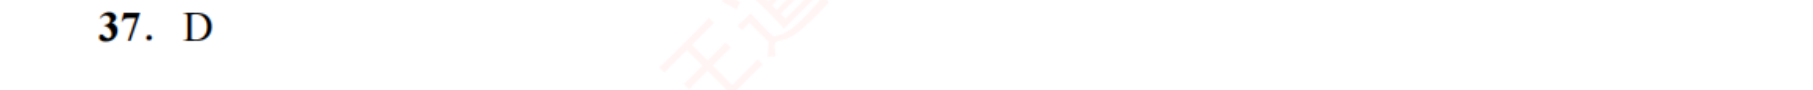
\includegraphics[width=161.13mm,height=180mm,keepaspectratio]{../solutions/assets/628066db7e21991b1bbc8c07.png}\par\smallskip
\par\medskip\noindent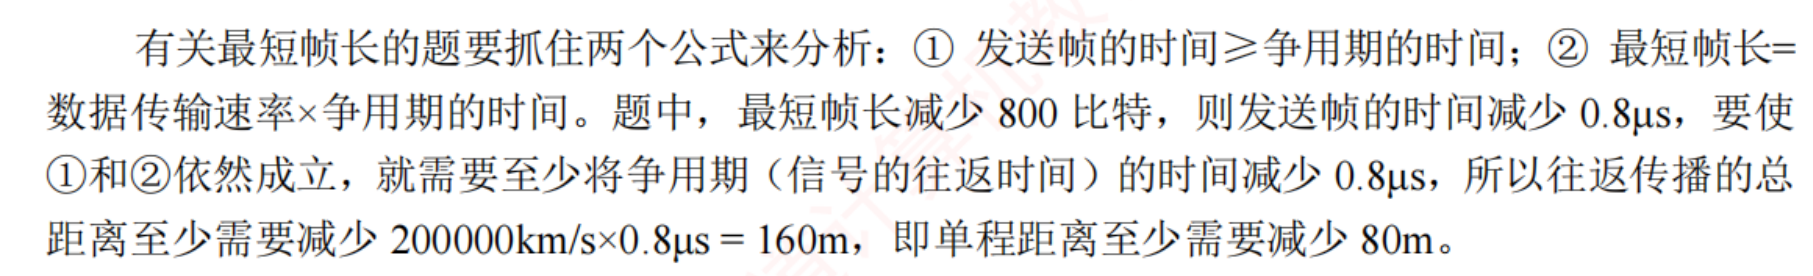
\includegraphics[width=161.13mm,height=180mm,keepaspectratio]{../solutions/assets/0686f52faa522b6a865e7995.png}\par\smallskip
\par\medskip\Needspace{5\baselineskip}\noindent\hypertarget{a:CN03-E09}{}\label{a:CN03-E09}\textbf{例 3-9}\quad B
\par\smallskip
\par\medskip\noindent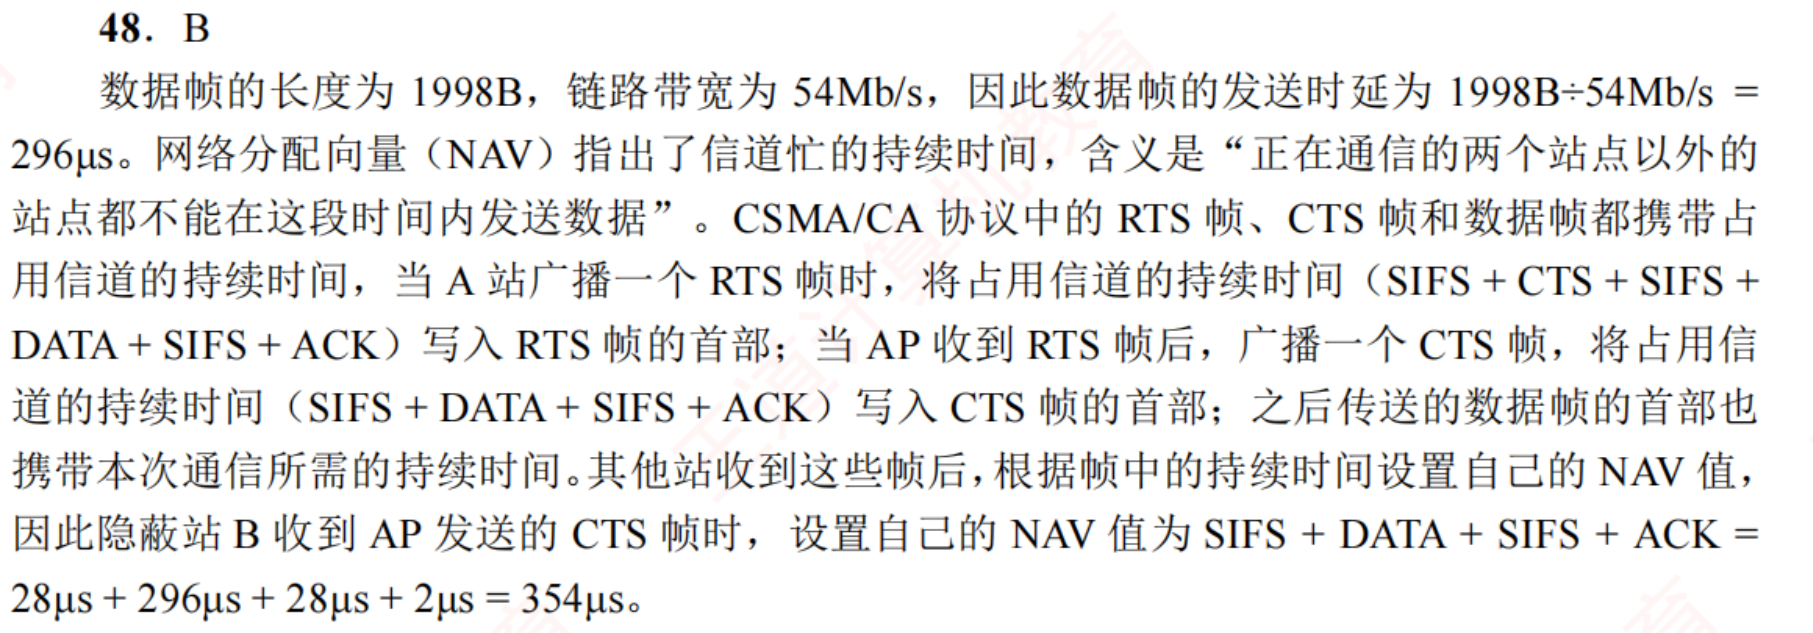
\includegraphics[width=161.13mm,height=180mm,keepaspectratio]{../solutions/assets/8b4c375de55a65f903be792b.png}\par\smallskip
\par\medskip\Needspace{5\baselineskip}\noindent\hypertarget{a:CN03-E10}{}\label{a:CN03-E10}\textbf{例 3-10}\quad A
\par\smallskip
\par\medskip\noindent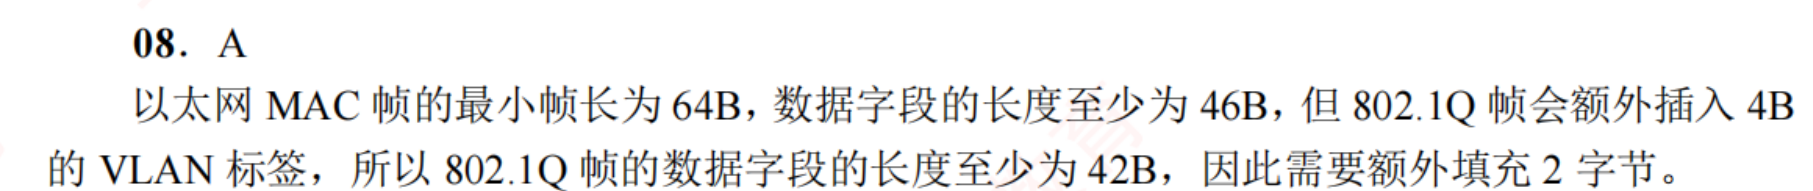
\includegraphics[width=161.13mm,height=180mm,keepaspectratio]{../solutions/assets/332cafd27f48df70206fed62.png}\par\smallskip
\par\medskip\Needspace{5\baselineskip}\noindent\hypertarget{a:CN03-E11}{}\label{a:CN03-E11}\textbf{例 3-11}\quad B
\par\smallskip
\par\medskip\noindent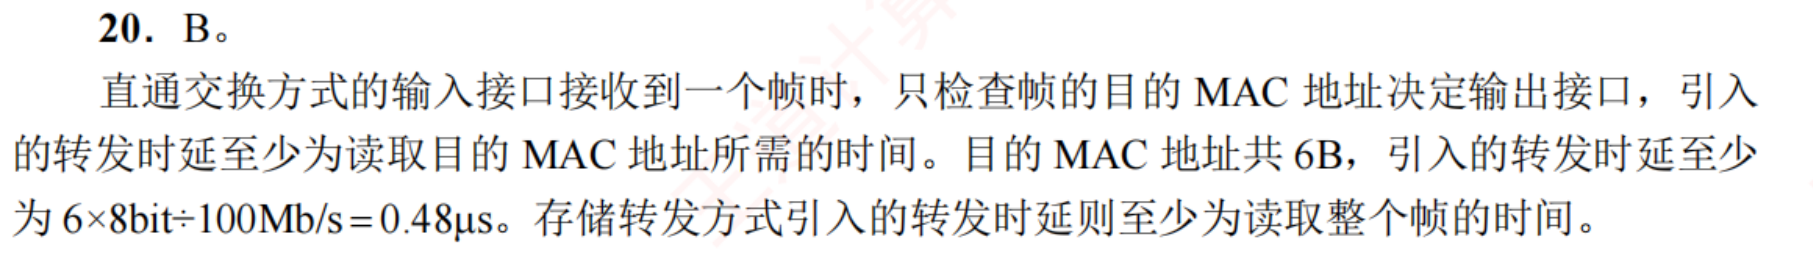
\includegraphics[width=161.13mm,height=180mm,keepaspectratio]{../solutions/assets/81d572eb1af3901ceb2fbae5.png}\par\smallskip
\par\medskip\Needspace{5\baselineskip}\noindent\hypertarget{a:CN03-E12}{}\label{a:CN03-E12}\textbf{例 3-12}\quad （1）3帧；（2）5帧，首\(S_{5,2}\)、末\(S_{1,2}\)；（3）3帧，首\(S_{2,3}\)；（4）50\%。
\par\smallskip
读题时先分清两条状态线：收到帧的确认序号决定``我发出的哪些帧已被确认''；收到帧的发送序号决定``我下次应捎带哪个确认号''。GBN的接收窗口为1，收到失序帧不能跳过缺口向前确认。序号空间为\(2^3=8\)，发送窗口最多为7，所有序号按模8回绕。

图(a)最后收到\(R_{3,3}\)。其确认号3累计确认甲方序号0、1、2已正确到达，因此第（1）问为3帧：\(S_{0,0}\)、\(S_{1,0}\)、\(S_{2,0}\)。不能因它的发送序号为3，便推断甲方也收齐了乙方0～3号帧：甲方依次正确收到\(R_{0,1}\)、\(R_{1,3}\)，随后缺少乙方2号帧，\(R_{3,3}\)作为失序帧被丢弃，所以甲方仍希望收到乙方2号帧。

此时甲方已发送到\(S_{4,1}\)，未确认的是发送序号3、4两帧。7个窗口位置中还剩\(7-2=5\)个；下一发送序号从5开始，捎带确认号始终为2，故第（2）问可发送\(S_{5,2}\)、\(S_{6,2}\)、\(S_{7,2}\)、\(S_{0,2}\)、\(S_{1,2}\)，首帧为\(S_{5,2}\)，末帧为\(S_{1,2}\)。回绕后的0、1是新一轮数据，不能与已经确认的旧0、1混为一谈。

图(b)乙方最后通告确认号2，意味着甲方0、1号已确认，2、3、4号仍未确认。\(S_{2,0}\)超时触发从最早未确认帧开始的后退重传，因此第（3）问重发3帧。甲方此时已按序收到乙方\(R_{2,2}\)，期待乙方下一帧为3，故重传首帧应更新捎带确认号，写成\(S_{2,3}\)；随后为\(S_{3,3}\)、\(S_{4,3}\)，不能照抄旧帧的确认号0。

第（4）问须保留捎带确认帧的发送时间。发送一个数据帧需\(T_d=1000\times8/(100\times10^6)=0.08\) ms；确认也装在1000 B的数据帧中，\(T_a=0.08\) ms。沿用教材模型：题目中的RTT表示往返传播时延；从发送首帧到完整收到其确认，周期为\(T_d+\mathrm{RTT}+T_a=1.12\) ms。最多连续发7帧，故\(U_{\max}=7\times0.08/1.12=50\%\)。全双工允许两个方向同时工作，但本题求甲方单方向利用率；也不能把长捎带确认当成长度可忽略的纯ACK。

\section*{网络层}
\par\medskip\Needspace{5\baselineskip}\noindent\hypertarget{a:CN04-E01}{}\label{a:CN04-E01}\textbf{例 4-1}\quad D
\par\smallskip
对Net1，经A、B、C、D的总距离为9、33、32、28，取9；Net2为20、45、42、34，取20；Net3为32、28、28、42，取28；Net4为44、40、20、30，取20。因此选 \textbf{D}。Net3经B、C并列最优，不影响距离答案；若另问下一跳，就须保留并列或按指定规则选择。

\par\medskip\Needspace{5\baselineskip}\noindent\hypertarget{a:CN04-E02}{}\label{a:CN04-E02}\textbf{例 4-2}\quad B
\par\smallskip
\par\medskip\noindent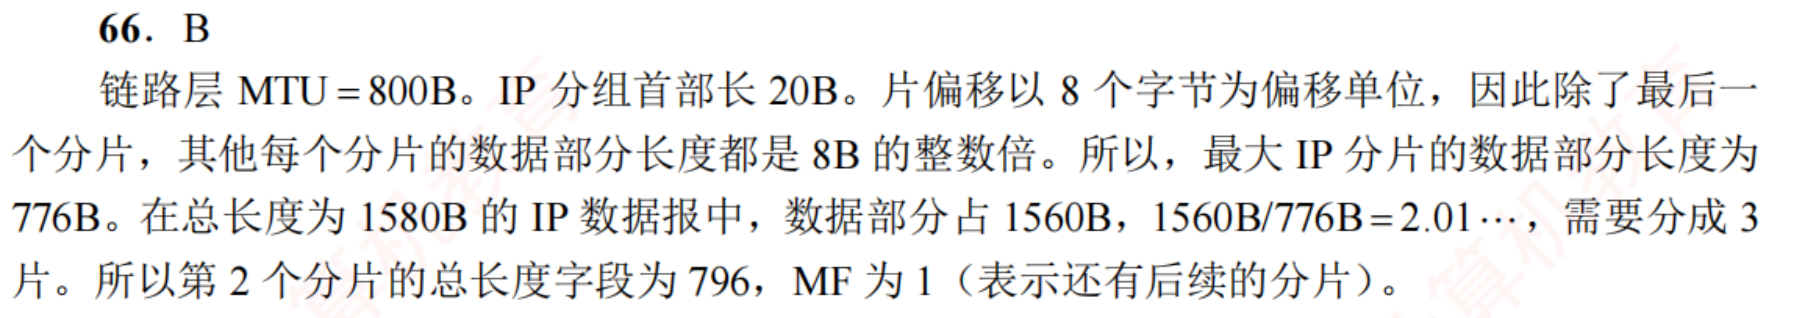
\includegraphics[width=161.13mm,height=180mm,keepaspectratio]{../solutions/assets/b568fec0433f1203a713884c.png}\par\smallskip
\par\medskip\Needspace{5\baselineskip}\noindent\hypertarget{a:CN04-E03}{}\label{a:CN04-E03}\textbf{例 4-3}\quad B
\par\smallskip
\par\medskip\noindent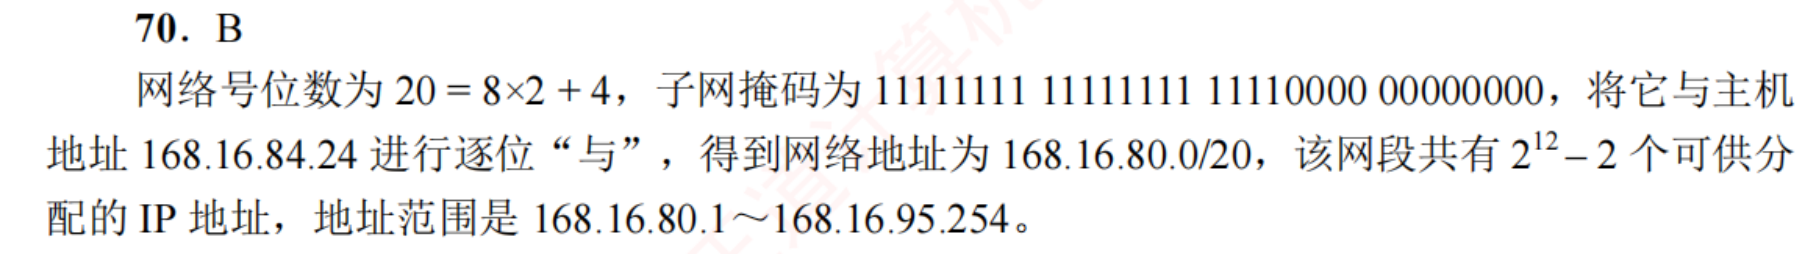
\includegraphics[width=161.13mm,height=180mm,keepaspectratio]{../solutions/assets/22da759fe9a73fcaac5a149e.png}\par\smallskip
\par\medskip\Needspace{5\baselineskip}\noindent\hypertarget{a:CN04-E04}{}\label{a:CN04-E04}\textbf{例 4-4}\quad B
\par\smallskip
\par\medskip\noindent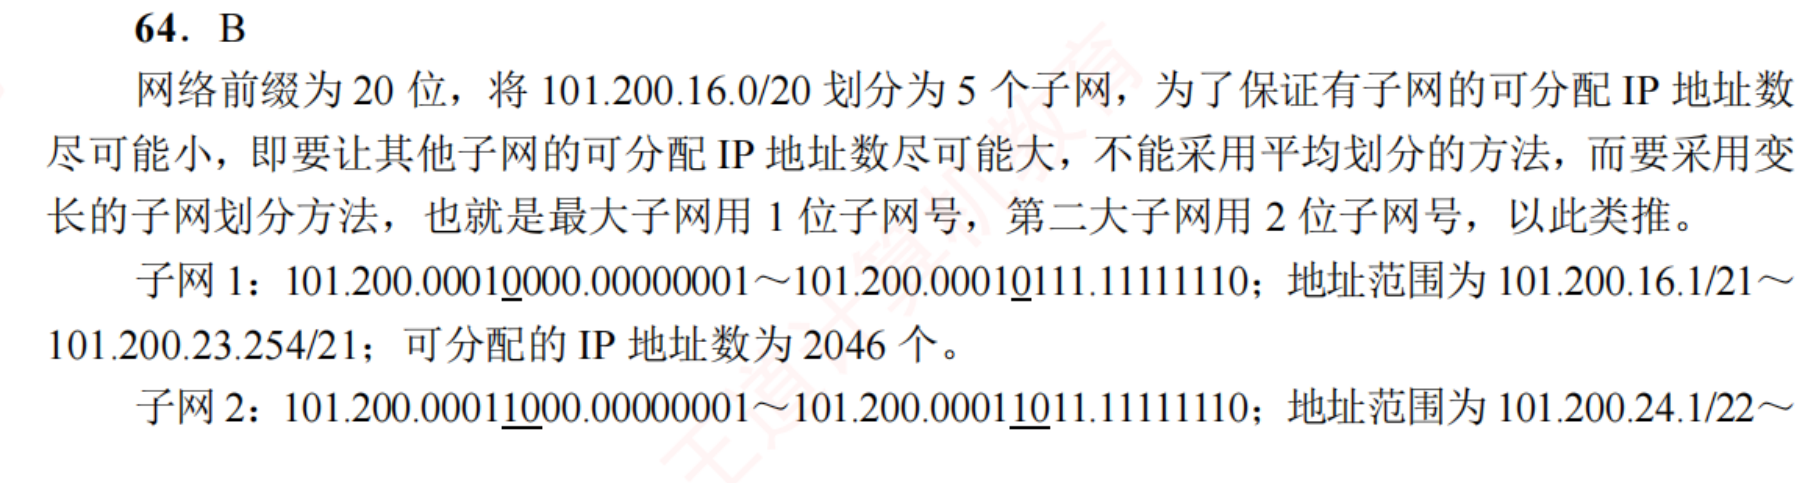
\includegraphics[width=161.13mm,height=180mm,keepaspectratio]{../solutions/assets/815d4c0902d26436959cef0a.png}\par\smallskip
\par\medskip\noindent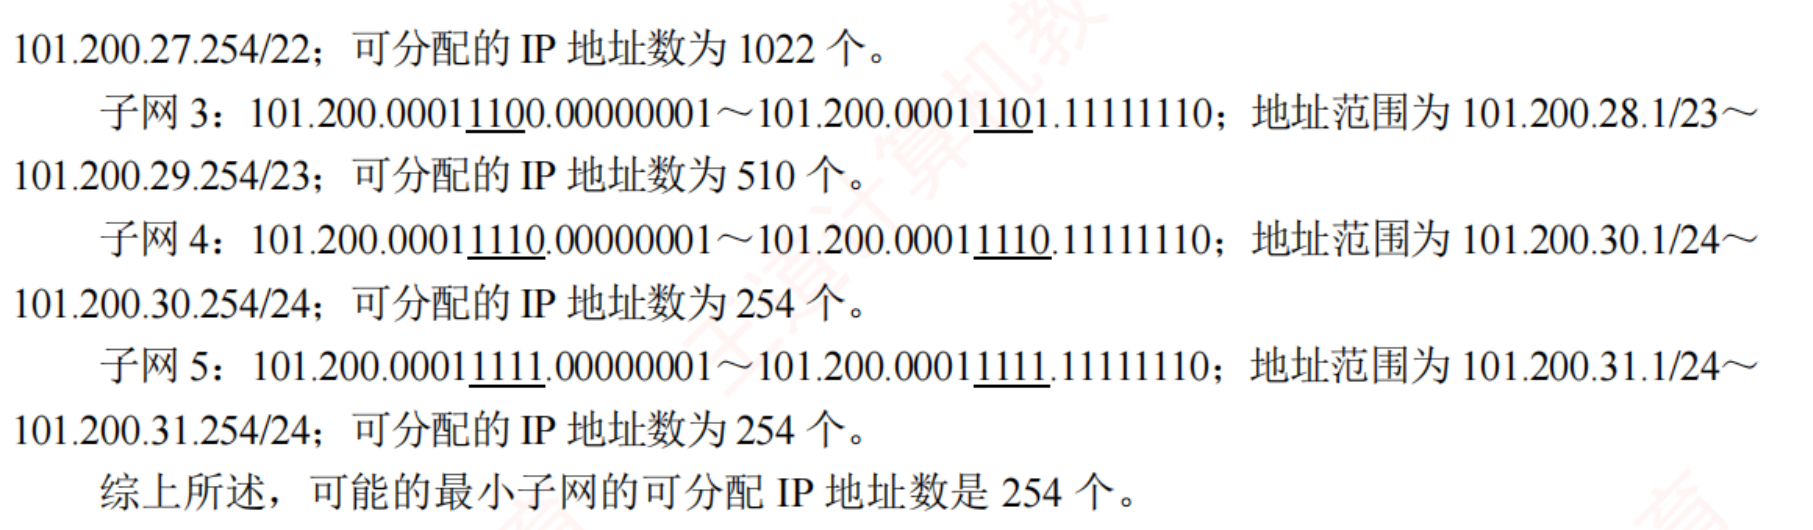
\includegraphics[width=161.13mm,height=180mm,keepaspectratio]{../solutions/assets/a151c17cb5df1cc83d65df2b.png}\par\smallskip
\par\medskip\Needspace{5\baselineskip}\noindent\hypertarget{a:CN04-E05}{}\label{a:CN04-E05}\textbf{例 4-5}\quad C
\par\smallskip
\par\medskip\noindent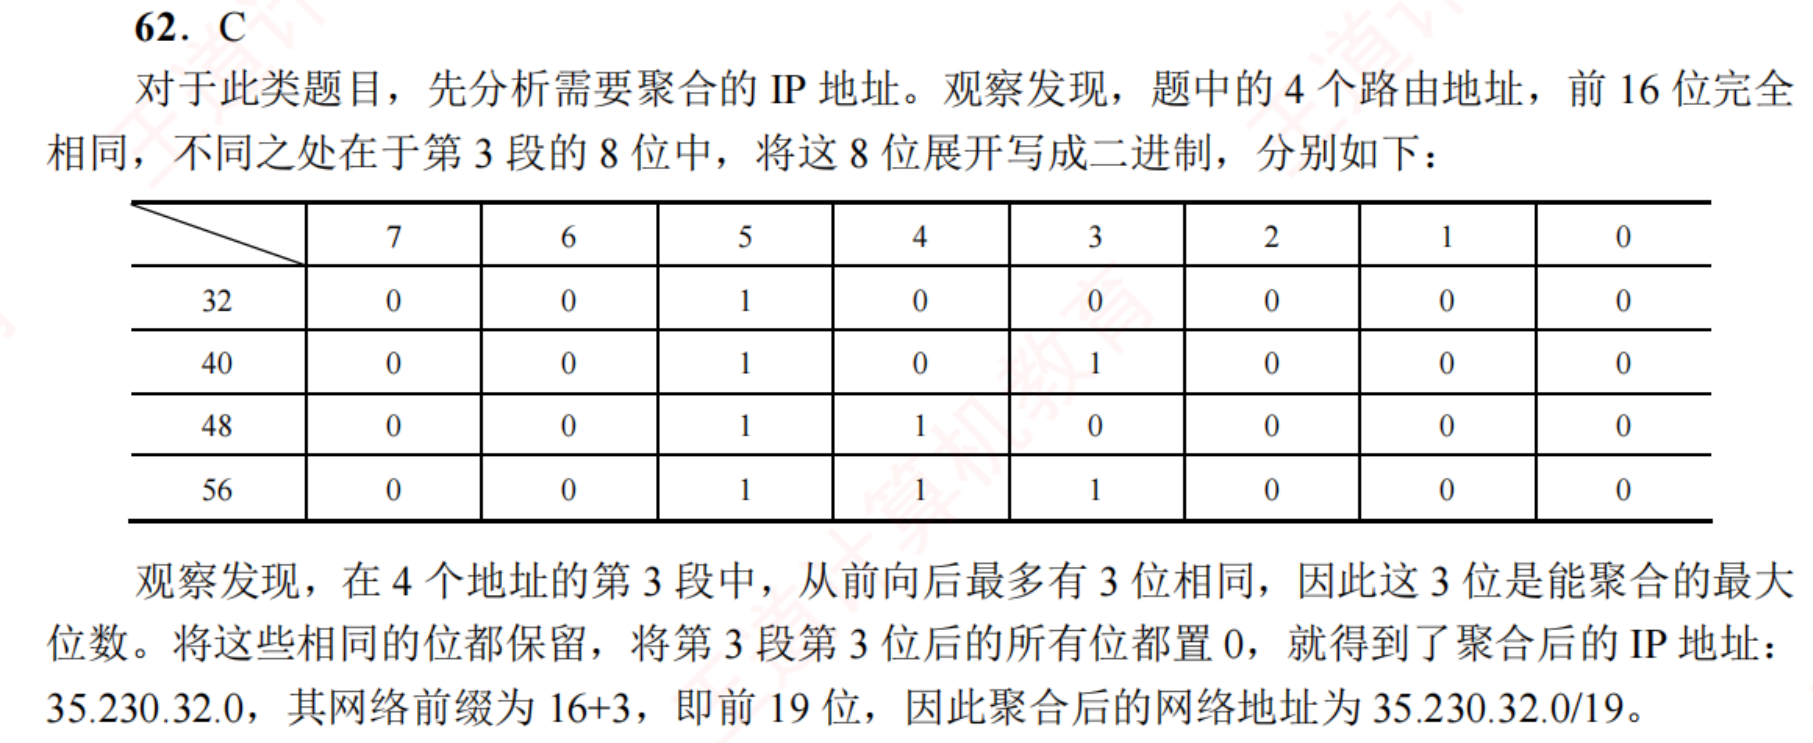
\includegraphics[width=161.13mm,height=180mm,keepaspectratio]{../solutions/assets/81d3d6987585c9df37dd602c.png}\par\smallskip
\par\medskip\Needspace{5\baselineskip}\noindent\hypertarget{a:CN04-E06}{}\label{a:CN04-E06}\textbf{例 4-6}\quad B
\par\smallskip
\par\medskip\noindent
\includegraphics[width=161.13mm,height=180mm,keepaspectratio]{../solutions/assets/9b81193d1b07f21358c2e99a.png}\par\smallskip
\par\medskip\Needspace{5\baselineskip}\noindent\hypertarget{a:CN04-E07}{}\label{a:CN04-E07}\textbf{例 4-7}\quad C
\par\smallskip
H仅收到地址提议，尚未获得192.168.5.9的使用确认。初始选择阶段Request使用源0.0.0.0、目的255.255.255.255，按``目的、源''的设问顺序选 \textbf{C}。服务器的单播地址不是这一步的目的IP地址。

图中Request框沿用原题的 \texttt{yiaddr} 标注。按DHCP规范，客户端此阶段申请的地址实际由Requested IP Address选项携带，客户端发出的 \texttt{yiaddr} 为0。图中的192.168.5.9应理解为待申请地址信息，不能据这个标注推出H已经能用它作IP源地址。Offer中的 \texttt{yiaddr} 才是服务器提出的地址。

\par\medskip\Needspace{5\baselineskip}\noindent\hypertarget{a:CN04-E08}{}\label{a:CN04-E08}\textbf{例 4-8}\quad C
\par\smallskip
\par\medskip\noindent
\includegraphics[width=161.13mm,height=180mm,keepaspectratio]{../solutions/assets/4e1570dea20757ba05e26a38.png}\par\smallskip
\par\medskip\Needspace{5\baselineskip}\noindent\hypertarget{a:CN04-E09}{}\label{a:CN04-E09}\textbf{例 4-9}\quad D
\par\smallskip
\par\medskip\noindent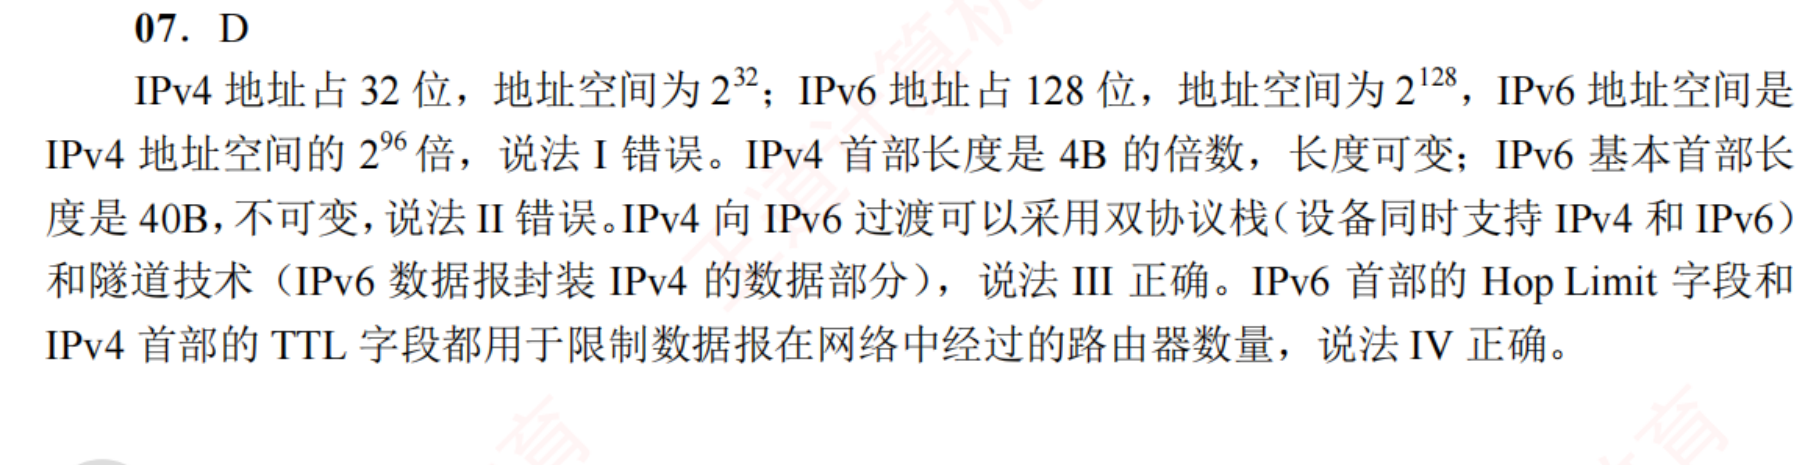
\includegraphics[width=161.13mm,height=180mm,keepaspectratio]{../solutions/assets/c74d157a6c6695c795c5b108.png}\par\smallskip
\par\medskip\Needspace{5\baselineskip}\noindent\hypertarget{a:CN04-E10}{}\label{a:CN04-E10}\textbf{例 4-10}\quad （1）192.168.1.127，192.168.1.128/25，45台；（2）2片，796 B与724 B。
\par\smallskip
``均分一个\texttt{/24}''先确定两个\texttt{/25}，每个块有128个地址，再利用已经分配的地址识别哪一块属于哪个部门。销售部\texttt{.1～.20}在192.168.1.0/25内，广播地址为\textbf{192.168.1.127}；技术部\texttt{.129～.208}在\textbf{192.168.1.128/25}内。技术部可用地址有\(128-2=126\)个，已分配主机数为\(208-129+1=80\)，F1的\texttt{.254}还占1个，因此还可连接\(126-80-1=\mathbf{45}\)台主机。路由器接口不是额外的一台用户主机，但会占用同一子网的可用地址。

分片计算从原IP数据部分开始：\(1500-20=1480\) B。F1所在链路每片总长不能超过800 B，扣首部后最多780 B；非末片数据长度又必须是8 B的整数倍，故最大数据量为\(\lfloor780/8\rfloor\times8=\mathbf{776}\) B。余下\(1480-776=704\) B，一片即可容纳，所以最少2片。

\begin{longtable}[]{@{}lrrl@{}}
\toprule\noalign{}
分片 & 数据长度/B & IP总长度/B & 片偏移（8 B单位）与MF \\
\midrule\noalign{}
\endhead
\bottomrule\noalign{}
\endlastfoot
第一片 & 776 & 796 & 偏移0，MF=1 \\
第二片 & 704 & 724 & 偏移97，MF=0 \\
\end{longtable}

第二片偏移是\(776/8=97\)，它累计的是原数据的位置，不加第一片首部。末片不要求数据长度继续凑满776 B，所有片的数据长度相加仍为1480 B。

\par\medskip\Needspace{5\baselineskip}\noindent\hypertarget{a:CN04-E11}{}\label{a:CN04-E11}\textbf{例 4-11}\quad 3条路由；目的194.17.20.200走E0；域间BGP，由TCP承载。
\par\smallskip
先按出口分组，再分别求可用汇总前缀。经S0到达的153.14.5.0/25、153.14.5.128/25恰好拼成153.14.5.0/24，下一跳为R1的153.14.3.2。经S1到达的194.17.20.0/25与194.17.21.0/24可用194.17.20.0/23覆盖，但这个\texttt{/23}也包含E0直连的194.17.20.128/25，必须保留该更具体条目，让最长前缀匹配处理例外。

\begin{longtable}[]{@{}lll@{}}
\toprule\noalign{}
目的网络 & 下一跳 & 接口 \\
\midrule\noalign{}
\endhead
\bottomrule\noalign{}
\endlastfoot
153.14.5.0/24 & 153.14.3.2 & S0 \\
194.17.20.0/23 & 194.17.24.2 & S1 \\
194.17.20.128/25 & ---（直连） & E0 \\
\end{longtable}

这3条分别承担三个不同出口，已不能在保持全部转发结果的前提下继续合并。第二条覆盖较宽范围，E0的更具体项处理直连例外。若删除E0例外，原本应直达的分组就会误发给R3。

194.17.20.200同时匹配\texttt{194.17.20.0/23}和\texttt{194.17.20.128/25}；比较前缀长度25与23，选择\textbf{E0}，不依赖表项书写顺序。R1与R2属于不同自治系统，因此交换域间路由使用\textbf{BGP（BGP-4）}，BGP报文由\textbf{TCP}承载。自治系统内部使用何种IGP，不改变这条跨AS邻接的协议选择。

\par\medskip\Needspace{5\baselineskip}\noindent\hypertarget{a:CN04-E12}{}\label{a:CN04-E12}\textbf{例 4-12}\quad （1）OSPF；（2）16；（3）30 s、60 s；（4）eBGP/UPDATE、iBGP；（5）R14选R11，R15选R13。
\par\smallskip
第（1）问先检查协议的适用上限。RIP最大有效跳数为15，16即不可达，AS4的规模可能超出这一限制，应选\textbf{OSPF}。第（2）问问的是IP的TTL而非RIP度量：每经过一个路由器TTL减1，减至0便被丢弃。最多经过15个路由器后仍须至少剩1，故初始TTL至少为\textbf{16}。

第（3）问把每次交换视作一轮：本轮只能把交换前已知的路由传给相邻路由器，不能让新收到的信息在同一轮连续穿越全网。又因为首次交换定义为\(t=0\)，直连路由在此刻已经传给一跳邻居，不能额外再计一个30 s。

\begin{longtable}[]{@{}
  >{\raggedright\arraybackslash}p{(\columnwidth - 4\tabcolsep) * \real{0.3333}}
  >{\raggedright\arraybackslash}p{(\columnwidth - 4\tabcolsep) * \real{0.3333}}
  >{\raggedright\arraybackslash}p{(\columnwidth - 4\tabcolsep) * \real{0.3333}}@{}}
\toprule\noalign{}
\begin{minipage}[b]{\linewidth}\raggedright
距首次交换的时间
\end{minipage} & \begin{minipage}[b]{\linewidth}\raggedright
已正确获知210.2.3.0/24的路由器
\end{minipage} & \begin{minipage}[b]{\linewidth}\raggedright
已正确获知210.2.4.0/24的路由器
\end{minipage} \\
\midrule\noalign{}
\endhead
\bottomrule\noalign{}
\endlastfoot
0 s & R14、R11、R15 & R16、R15 \\
30 s & R11～R16全部 & R16、R15、R14、R13 \\
60 s & R11～R16全部 & R11～R16全部 \\
\end{longtable}

210.2.3.0/24直连R14，首次传给R11、R15，下一轮由它们传给R12、R13、R16，所以需\textbf{30 s}。210.2.4.0/24直连R16，首次仅传给R15，30 s时到R14、R13，60 s时才到R11、R12，所以需\textbf{60 s}。逐轮集合依赖题图中实际存在的边，不能擅自补上R13---R16。

第（4）问按会话两端是否同属一个AS区分：R44与R13分属AS4、AS1，用\textbf{eBGP}会话，通过\textbf{UPDATE}报文通告；R13向同属AS1的R14、R15传播可达性信息，用\textbf{iBGP}会话。BGP会话不要求所有对端在物理上直接相连。

第（5）问按本题无策略约束的教材选路模型，先比较AS\_PATH：经R11、R13的路径各含3个AS，经R12含4个，先排除R12。在其余属性相同的候选中，再比较AS内到出口的距离。R14到R11为1跳，到R13需经R15为2跳，选\textbf{R11}；R15到R13为1跳，到R11为2跳，选\textbf{R13}。真实BGP还受本地优先级等属性影响，本题给定条件并不支持把``AS数少、出口近''当成无条件覆盖所有策略的规则。

\par\medskip\Needspace{5\baselineskip}\noindent\hypertarget{a:CN04-E13}{}\label{a:CN04-E13}\textbf{例 4-13}\quad （1）0.24 s、200 kb/s、理想下界0.40 s；（2）8帧、4 bit；（3）作业区10.10.10.64/26，管理区10.10.10.0/26，生活区10.10.10.128/25。
\par\smallskip
单向路径要经过``地面\ensuremath{\to}卫星\ensuremath{\to}地面''两段。按本题采用的几何模型，每段链路的长度取卫星高度，单向传播时延\(T_p=2\times36000/300000=\mathbf{0.24\ s}\)。路径吞吐量受最慢链路限制，千兆以太网不能抬高200 kb/s的卫星瓶颈，因此H单方向最大吞吐量为\textbf{200 kb/s}；全双工表示反方向另有同样容量，不能在一次上传中相加成400 kb/s。

4000 B经卫星链路发送需\(4000\times8/200000=0.16\) s。首部忽略时，最后一比特从卫星链路发送端到接收端还要传播0.24 s，故教材模型给出的最短上传时间为\(0.16+0.24=\mathbf{0.40\ s}\)。这个400 ms还额外忽略了局域网的发送开销；题干给出的忽略项并不包含千兆链路上的发送与分帧，若要严格计入每段链路上的发送、分帧及存储转发，还需题目进一步指定相应条件。例如4000 B在一条1 Gb/s链路上仅串行发送也需32 μs。因此400 ms适合作为本题理想下界，不能视为所有实际以太网转发方式下的精确完成时间。

SLP每帧发送时延\(T_d=1500\times8/200000=60\) ms；ACK长度忽略，从开始发送首帧到收到其确认需\(60+2\times240=540\) ms。设窗口为\(W\)，利用率\(U=\min(1,60W/540)\)；要求\(U\ge0.8\)，得到\(W\ge7.2\)，向上取整为\textbf{8帧}。GBN接收窗口为1，需\(2^k\ge W+1=9\)，所以序号字段最少\textbf{4 bit}。3 bit虽然有8个序号，却只能支持最大7帧的GBN发送窗口；其利用率\(7/9\approx77.78\%\)，达不到要求。

最后按可用主机数决定块大小。生活区需\(2^7-2=126\)个可用地址，至少占\texttt{/25}；另两区各需\(2^6-2=62\)个，至少占\texttt{/26}。三块恰好用完\(128+64+64=256\)个地址。H的10.10.10.33/26锁定管理区为10.10.10.0/26；生活区的\texttt{/25}必须按128地址边界对齐，且不能与管理区重叠，只能取10.10.10.128/25，留下10.10.10.64/26给作业区。

\begin{longtable}[]{@{}lllr@{}}
\toprule\noalign{}
子网 & CIDR地址 & 可用地址范围 & 可用数量 \\
\midrule\noalign{}
\endhead
\bottomrule\noalign{}
\endlastfoot
作业区 & \textbf{10.10.10.64/26} & 10.10.10.65～10.10.10.126 & 62 \\
管理区 & \textbf{10.10.10.0/26} & 10.10.10.1～10.10.10.62 & 62 \\
生活区 & \textbf{10.10.10.128/25} & 10.10.10.129～10.10.10.254 & 126 \\
\end{longtable}

\section*{传输层}
\par\medskip\Needspace{5\baselineskip}\noindent\hypertarget{a:CN05-E01}{}\label{a:CN05-E01}\textbf{例 5-1}\quad B
\par\smallskip
\par\medskip\noindent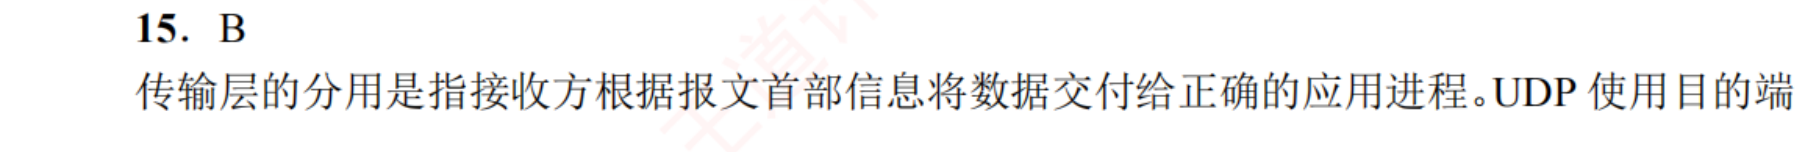
\includegraphics[width=161.13mm,height=180mm,keepaspectratio]{../solutions/assets/230826e395e08a7732448510.png}\par\smallskip
\par\medskip\noindent
\includegraphics[width=161.13mm,height=180mm,keepaspectratio]{../solutions/assets/321584685bd29ebbe6113df6.png}\par\smallskip
\par\medskip\Needspace{5\baselineskip}\noindent\hypertarget{a:CN05-E02}{}\label{a:CN05-E02}\textbf{例 5-2}\quad C
\par\smallskip
\par\medskip\noindent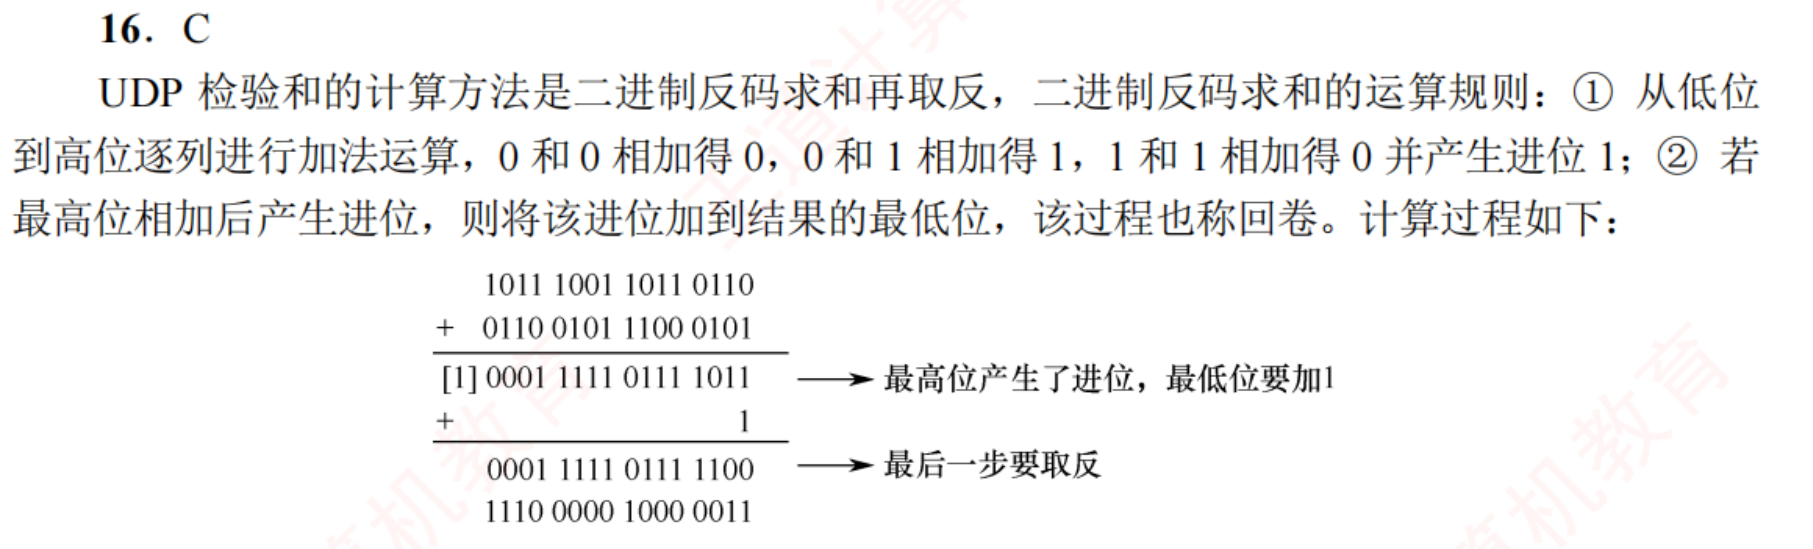
\includegraphics[width=161.13mm,height=180mm,keepaspectratio]{../solutions/assets/d7d92d19be807314e5b63ffb.png}\par\smallskip
\par\medskip\Needspace{5\baselineskip}\noindent\hypertarget{a:CN05-E03}{}\label{a:CN05-E03}\textbf{例 5-3}\quad D
\par\smallskip
\par\medskip\noindent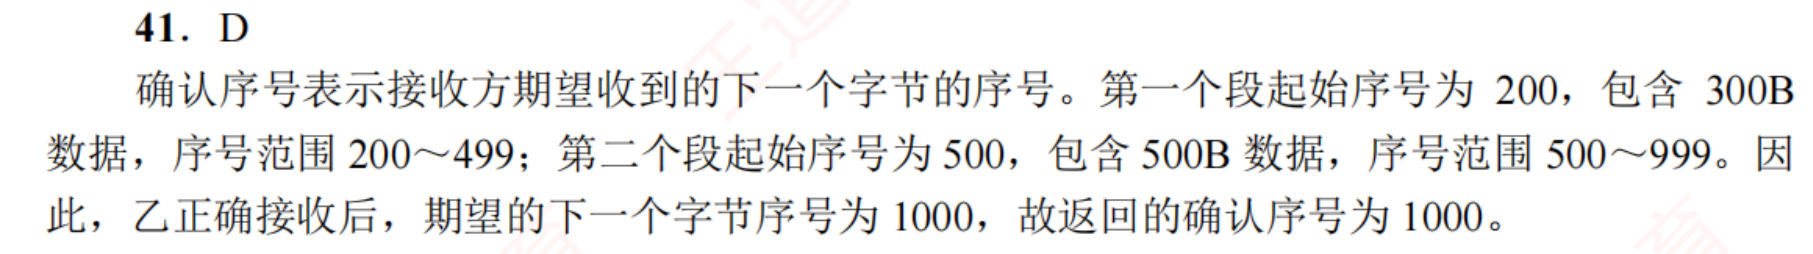
\includegraphics[width=161.13mm,height=180mm,keepaspectratio]{../solutions/assets/fb4a17d51d5da99b4054876b.png}\par\smallskip
\par\medskip\Needspace{5\baselineskip}\noindent\hypertarget{a:CN05-E04}{}\label{a:CN05-E04}\textbf{例 5-4}\quad D
\par\smallskip
\par\medskip\noindent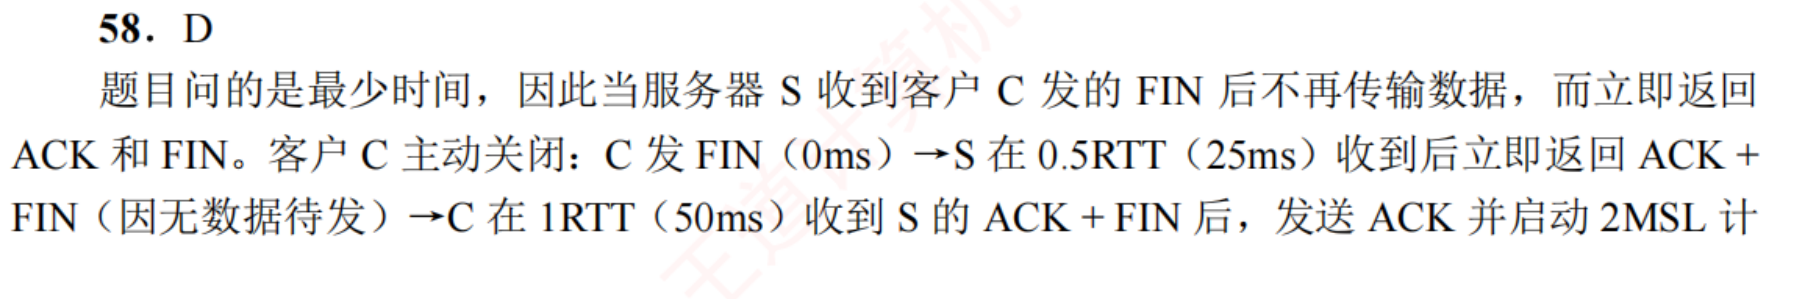
\includegraphics[width=161.13mm,height=180mm,keepaspectratio]{../solutions/assets/cc75e54b46dec4e72a54be8f.png}\par\smallskip
\par\medskip\noindent
\includegraphics[width=161.13mm,height=180mm,keepaspectratio]{../solutions/assets/5597bb39f6b2489d66691472.png}\par\smallskip
\par\medskip\Needspace{5\baselineskip}\noindent\hypertarget{a:CN05-E05}{}\label{a:CN05-E05}\textbf{例 5-5}\quad D
\par\smallskip
\par\medskip\noindent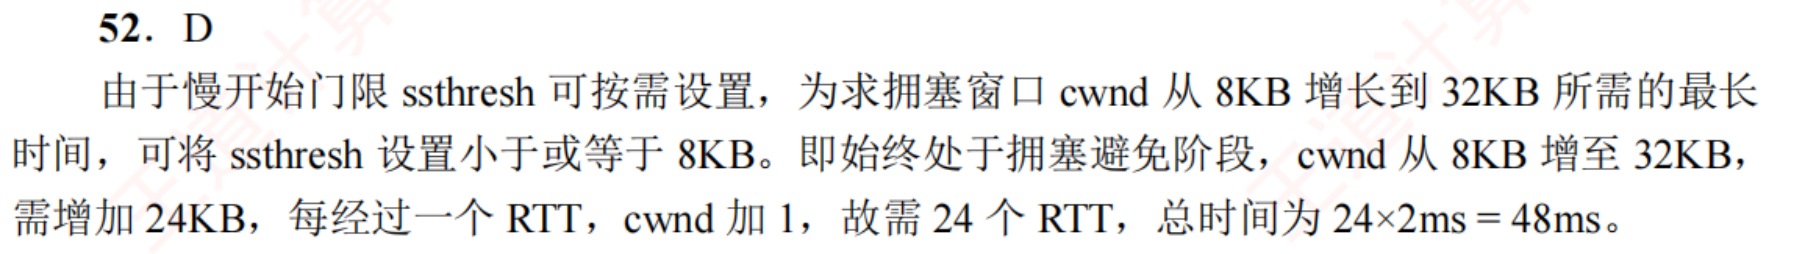
\includegraphics[width=161.13mm,height=180mm,keepaspectratio]{../solutions/assets/8783487cfe6b7209aaa19242.png}\par\smallskip
\par\medskip\Needspace{5\baselineskip}\noindent\hypertarget{a:CN05-E06}{}\label{a:CN05-E06}\textbf{例 5-6}\quad A
\par\smallskip
第一段seq=2001覆盖2001～3000，第二段seq=3001覆盖3001～4000。返回ack\_seq=3001只累计确认第一段，第二段的1000 B仍在途。乙段的seq=4001属于乙\ensuremath{\to}甲方向，不能拿它确认甲发出的字节。

甲原cwnd为2000 B，小于门限8000 B，收到一份对新数据的确认后，按题设慢开始增加1 MSS，cwnd变为3000 B；rwnd通告为4000 B，总发送额度取3000 B。减去在途1000 B，尚可新发2000 B，即2段，选 \textbf{A}。对应允许的甲方发送范围从3001起共3000 B，其中3001～4000已经发出，4001～6000还可新发。

\par\medskip\Needspace{5\baselineskip}\noindent\hypertarget{a:CN05-E07}{}\label{a:CN05-E07}\textbf{例 5-7}\quad A
\par\smallskip
\par\medskip\noindent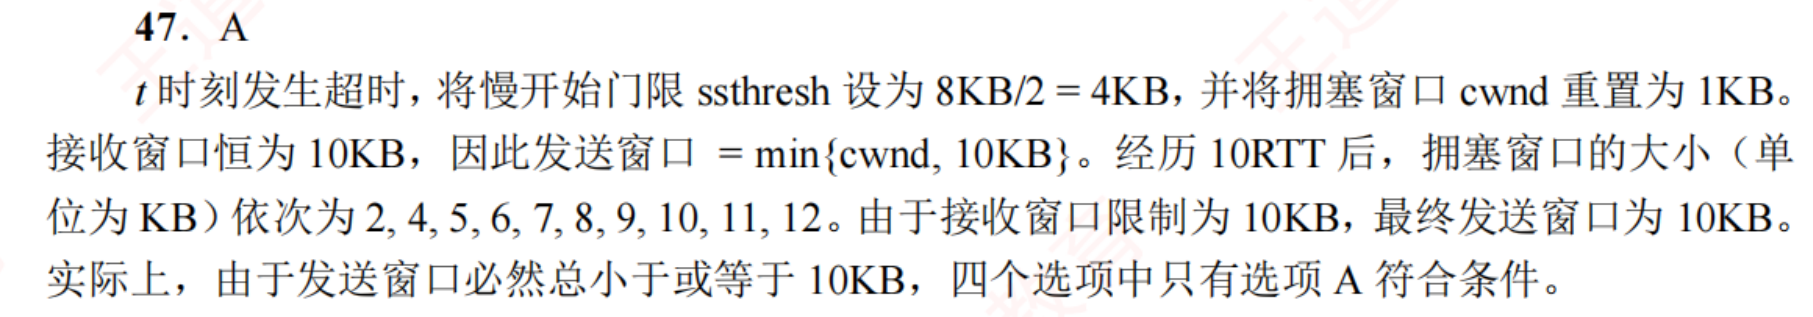
\includegraphics[width=161.13mm,height=180mm,keepaspectratio]{../solutions/assets/b117465bf5d3cd7bb8536b72.png}\par\smallskip
\par\medskip\Needspace{5\baselineskip}\noindent\hypertarget{a:CN05-E08}{}\label{a:CN05-E08}\textbf{例 5-8}\quad （1）H发送1、3、4；握手1、2、3；填充3、5；（2）16 B；（3）15个路由器。
\par\smallskip
按``IP长度\ensuremath{\to}TCP起点\ensuremath{\to}控制位\ensuremath{\to}序号确认号''顺序解码。所有分组首字节45表示IPv4、IHL=5，即20 B IP首部，TCP从第21字节开始。1、3、4号的源地址\texttt{c0\ a8\ 00\ 08}为192.168.0.8，因此\textbf{H发送的是1、3、4号}；2、5号的源地址为S。

\begin{longtable}[]{@{}lrrl@{}}
\toprule\noalign{}
编号 & IP总长/B & TCP首长/B & TCP标志 \\
\midrule\noalign{}
\endhead
\bottomrule\noalign{}
\endlastfoot
1 & 48 & 28 & SYN \\
2 & 48 & 28 & SYN、ACK \\
3 & 40 & 20 & ACK \\
4 & 56 & 20 & PSH、ACK \\
5 & 40 & 20 & ACK \\
\end{longtable}

\begin{longtable}[]{@{}lllr@{}}
\toprule\noalign{}
编号 & seq（十六进制） & ack（十六进制） & 应用数据/B \\
\midrule\noalign{}
\endhead
\bottomrule\noalign{}
\endlastfoot
1 & 846b41c5 & 00000000（ACK=0） & 0 \\
2 & e0599fef & 846b41c6 & 0 \\
3 & 846b41c6 & e0599ff0 & 0 \\
4 & 846b41c6 & e0599ff0 & 16 \\
5 & e0599ff0 & 846b41d6 & 0 \\
\end{longtable}

1号的TCP数据偏移高半字节为7，首部长\(7\times4=28\) B；控制字节02置SYN。2号的控制字节12同时置了SYN与ACK，确认H的初始序号加1；3号的控制字节10只置ACK，确认S的初始序号加1。因此\textbf{1、2、3号完成三次握手}，SYN分别消耗一个序号，第三次纯ACK不额外消耗序号。捕获表只给前40 B，1、2号的8 B TCP选项没有完整列出，但长度字段足以判定它们没有应用数据。

快速以太网沿用无标签以太网数据字段至少46 B的限制，判断填充应比较\textbf{整个IP分组}与46 B，不能只比较TCP数据。3、5号IP总长\texttt{0028}为40 B，均需补\(46-40=6\) B；1、2号为48 B、4号为56 B，均不需补。因此填充的是\textbf{3、5号}，每个形成\(14+40+6+4=64\) B的最短MAC帧。填充不计入IP总长度，更不占TCP字节序号。

第（2）问利用累计确认而不是把40字节截取范围当作完整数据。H首个应用字节的序号为SYN序号加1，即\texttt{846b41c6}；5号通告下一个期望序号\texttt{846b41d6}，所以S已按序收到\(\mathtt{846b41d6}-\mathtt{846b41c6}=\mathtt{10}=\mathbf{16}\) B应用数据。这也与4号的\(56-20-20=16\) B相符。

第（3）问先匹配报文身份。S行IP标识为\texttt{6811}，TCP序号、确认号与5号一致，对应H处的5号；途中的NAT可能改变目的地址与端口，不能因此误认为是另一个报文。S发出时TTL为\texttt{40}即64，H处为\texttt{31}即49，每经过一个路由器减1，故经过\(64-49=\mathbf{15}\)个路由器。交换机不减TTL。图中的其余校验和字节按来源保留；题目只截取了部分字节，选项与有效载荷并未给全，不能据此声称已经验证所有报文的完整校验和。

\par\medskip\Needspace{5\baselineskip}\noindent\hypertarget{a:CN05-E09}{}\label{a:CN05-E09}\textbf{例 5-9}\quad （1）SYN=ACK=1，ack=101；（2）rwnd=12 KB，cwnd=9 KB，发送窗口9 KB；（3）20581，163.84 kb/s；（4）300 ms。
\par\smallskip
第（1）问的第二次握手要同时表达``接受对方SYN''和``发出本方SYN''，所以\textbf{SYN=1、ACK=1、确认号=101}。初始序号100被SYN占用，首个数据字节从101开始。

第（2）问必须分别更新两种窗口。沿用教材模型：初始拥塞窗口为1 MSS，每个新数据段的ACK使慢开始窗口增加1 MSS。第8个数据确认到达后，\(cwnd=(1+8)\times1=\mathbf{9\ KB}\)，仍小于32 KB阈值；S已经缓存8 KB且未取出，通告\(rwnd=20-8=\mathbf{12\ KB}\)。发送窗口总额度为\(\min(cwnd,rwnd)=\mathbf{9\ KB}\)。如果题目问此时能再发送多少，还须扣除已经发出但未确认的数据，不能把9 KB直接当成新增发送量。

第（3）问要计到零窗口通告回到H3的时刻。每轮受拥塞窗口与剩余接收缓存共同限制，不能把慢开始序列无限写成1、2、4、8、16。

\begin{longtable}[]{@{}lrrr@{}}
\toprule\noalign{}
轮次 & 发送前cwnd/MSS & 尚余接收缓存/KB & 本轮发送/KB \\
\midrule\noalign{}
\endhead
\bottomrule\noalign{}
\endlastfoot
1 & 1 & 20 & 1 \\
2 & 2 & 19 & 2 \\
3 & 4 & 17 & 4 \\
4 & 8 & 13 & 8 \\
5 & 16 & 5 & 5 \\
\end{longtable}

\begin{longtable}[]{@{}lrl@{}}
\toprule\noalign{}
轮次 & 累计已接收/KB & 本轮确认到达时刻 \\
\midrule\noalign{}
\endhead
\bottomrule\noalign{}
\endlastfoot
1 & 1 & 1 RTT \\
2 & 3 & 2 RTT \\
3 & 7 & 3 RTT \\
4 & 15 & 4 RTT \\
5 & 20 & 5 RTT \\
\end{longtable}

第5轮只能再放入5 KB，S随后通告零窗口。下一个待发送字节的序号为\(101+20\times1024=\mathbf{20581}\)，这个值不因窗口暂时关闭而重置。计时为\(5\times200\mathrm{\ ms}=1\) s，平均速率为\(20\times1024\times8/1=\mathbf{163840\ bit/s}=\mathbf{163.84\ kb/s}\)。这里KB用1024、kb/s用1000；计时起点不包括握手，但终点包括最后一轮确认回传。

零窗口是接收方流量控制的结果，并不说明此前有数据丢失，也不要求按超时规则把cwnd重置为1。发送方可用持续计时器触发零窗口探测，以免窗口更新丢失后永久等待；探测本身不会使接收缓存腾空。在本题``始终不取数据''的条件下，不能假设经过一个RTT窗口便自动恢复。

第（4）问求S的释放时间。为取最短值，S收到H3的FIN后立即合并发出ACK和自己的FIN：H3的FIN到S用0.5 RTT，S的FIN到H3再用0.5 RTT，H3的最后ACK返回S再用0.5 RTT。S收到此ACK后进入CLOSED，故最短为\(1.5\mathrm{RTT}=\mathbf{300\ ms}\)。H3作为主动关闭方的TIME-WAIT等待属于另一端的计时，不能再加到S的300 ms上。

\section*{应用层}
\par\medskip\Needspace{5\baselineskip}\noindent\hypertarget{a:CN06-E01}{}\label{a:CN06-E01}\textbf{例 6-1}\quad C
\par\smallskip
计数主体是201.1.1.1，不是H4。最终地址在有效缓存中时，本地服务器不需向外查询，最少0次；完全无可用缓存，且相应各级分别委派时，可依次询问根、com、xyz.com、abc.xyz.com，共4次，选 \textbf{C}。H4向201.1.1.1的最初请求不是这台服务器``发出''的请求，不能加入。

``最多4次''采用原题的规范域名及逐级委派模型，不计别名链、失败重试或负载均衡额外查询。若改问主机发出几条请求，或所有层级均以递归方式向下转交，通信主体与计数就要重新列出，而不是照抄0、4。

\par\medskip\Needspace{5\baselineskip}\noindent\hypertarget{a:CN06-E02}{}\label{a:CN06-E02}\textbf{例 6-2}\quad A
\par\smallskip
\par\medskip\noindent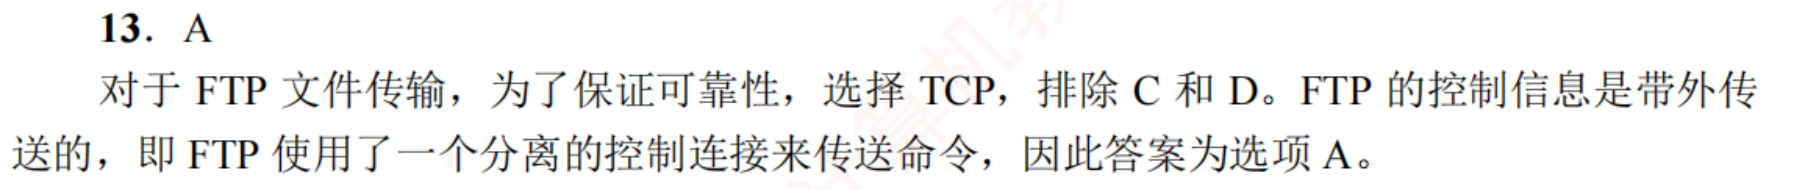
\includegraphics[width=161.13mm,height=180mm,keepaspectratio]{../solutions/assets/10b4b5c6ceab79c8710aef39.png}\par\smallskip
\par\medskip\Needspace{5\baselineskip}\noindent\hypertarget{a:CN06-E03}{}\label{a:CN06-E03}\textbf{例 6-3}\quad A
\par\smallskip
\par\medskip\noindent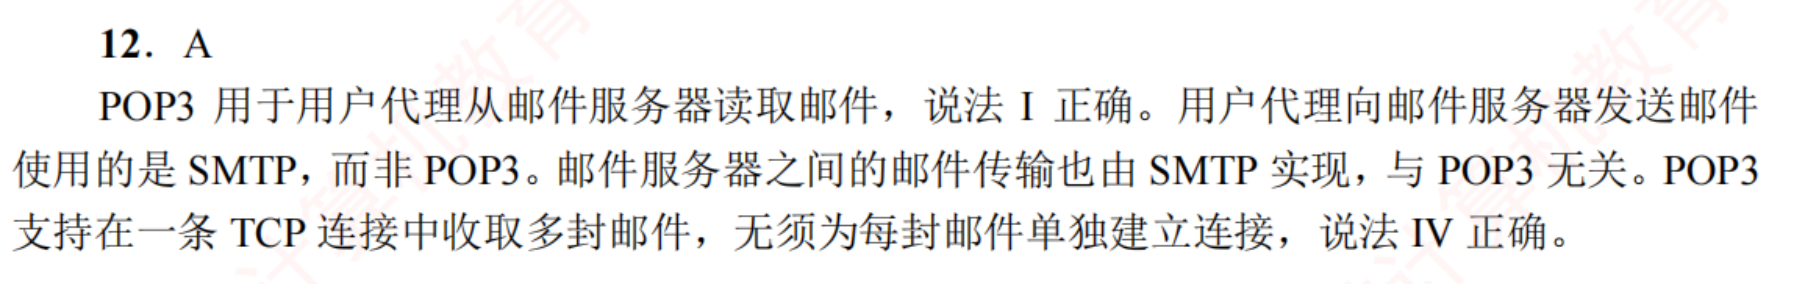
\includegraphics[width=161.13mm,height=180mm,keepaspectratio]{../solutions/assets/952dad39ebb217339c3ed384.png}\par\smallskip
\par\medskip\Needspace{5\baselineskip}\noindent\hypertarget{a:CN06-E04}{}\label{a:CN06-E04}\textbf{例 6-4}\quad D
\par\smallskip
\par\medskip\noindent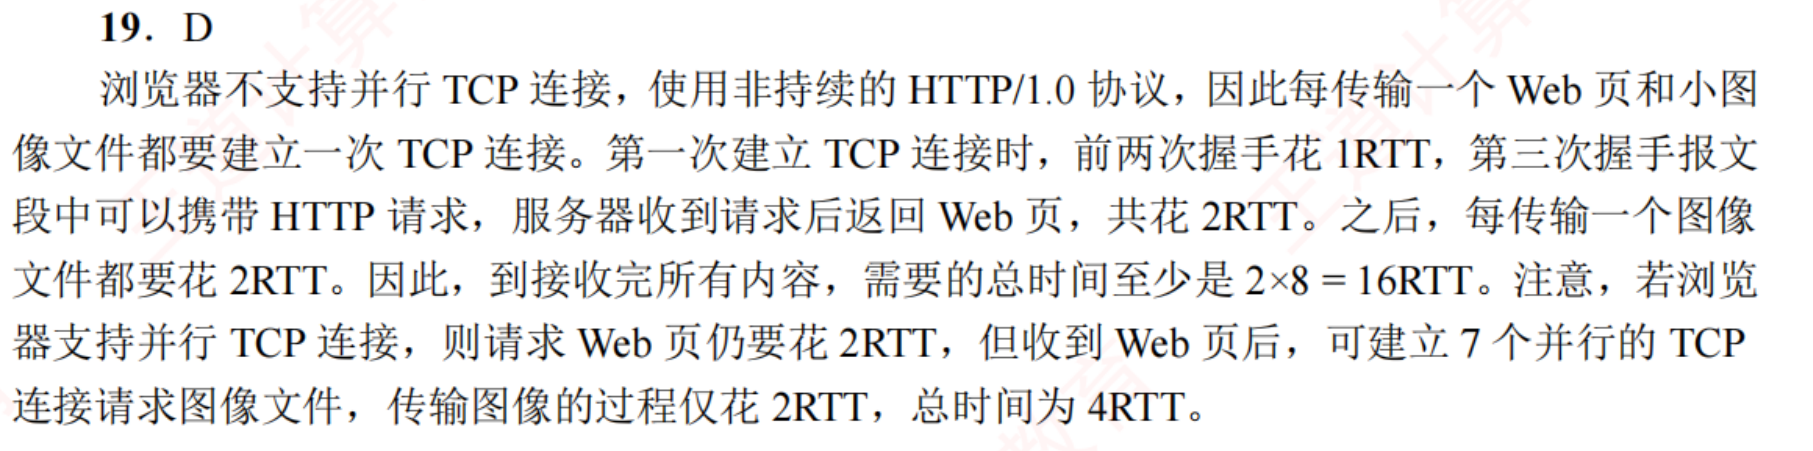
\includegraphics[width=161.13mm,height=180mm,keepaspectratio]{../solutions/assets/18a21ae7ed8b27de6b3ff109.png}\par\smallskip
\par\medskip\Needspace{5\baselineskip}\noindent\hypertarget{a:CN06-E05}{}\label{a:CN06-E05}\textbf{例 6-5}\quad A
\par\smallskip
\par\medskip\noindent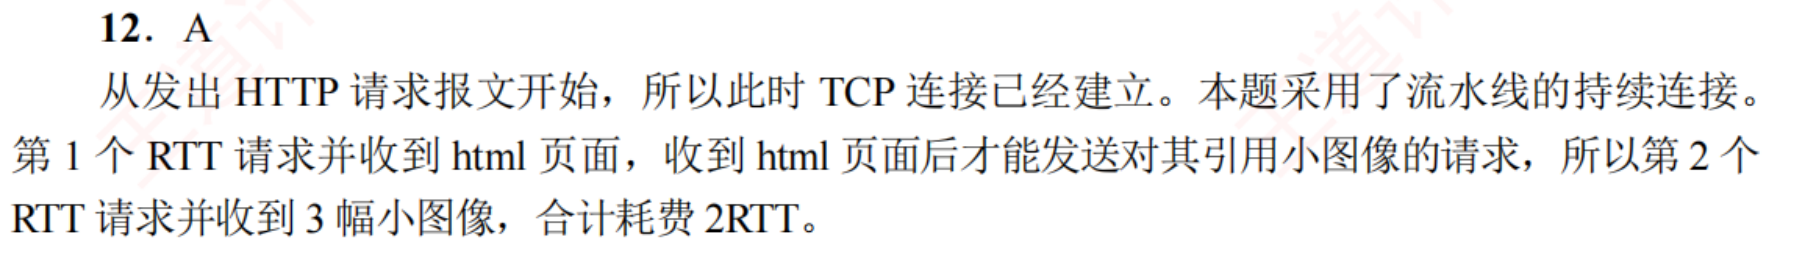
\includegraphics[width=161.13mm,height=180mm,keepaspectratio]{../solutions/assets/8afcf0778b0799383fee8d0b.png}\par\smallskip
\par\medskip\Needspace{5\baselineskip}\noindent\hypertarget{a:CN06-E06}{}\label{a:CN06-E06}\textbf{例 6-6}\quad D
\par\smallskip
采用题目首次取页面、尚未建立目标TCP连接的模型。有效DNS缓存命中时，不需要远程DNS往返，但TCP建立与HTTP请求响应各1RTT，最短20 ms。完全无所需缓存时，本地解析器依次询问根、com、abc.com权威服务器，增加3RTT；再取Web共5RTT=50 ms，选 \textbf{D}。主机与本地DNS之间的局域网时延已忽略，不能额外加一次10 ms。

如果题目再允许浏览器已缓存新鲜的HTML副本，可能无须访问服务器；若TCP已经建立，也会少一个握手往返。这些是改变原题模型的附加条件，不能在原题中任意引入后声称存在另一个更短答案。

\par\medskip\Needspace{5\baselineskip}\noindent\hypertarget{a:CN06-E07}{}\label{a:CN06-E07}\textbf{例 6-7}\quad B
\par\smallskip
\par\medskip\noindent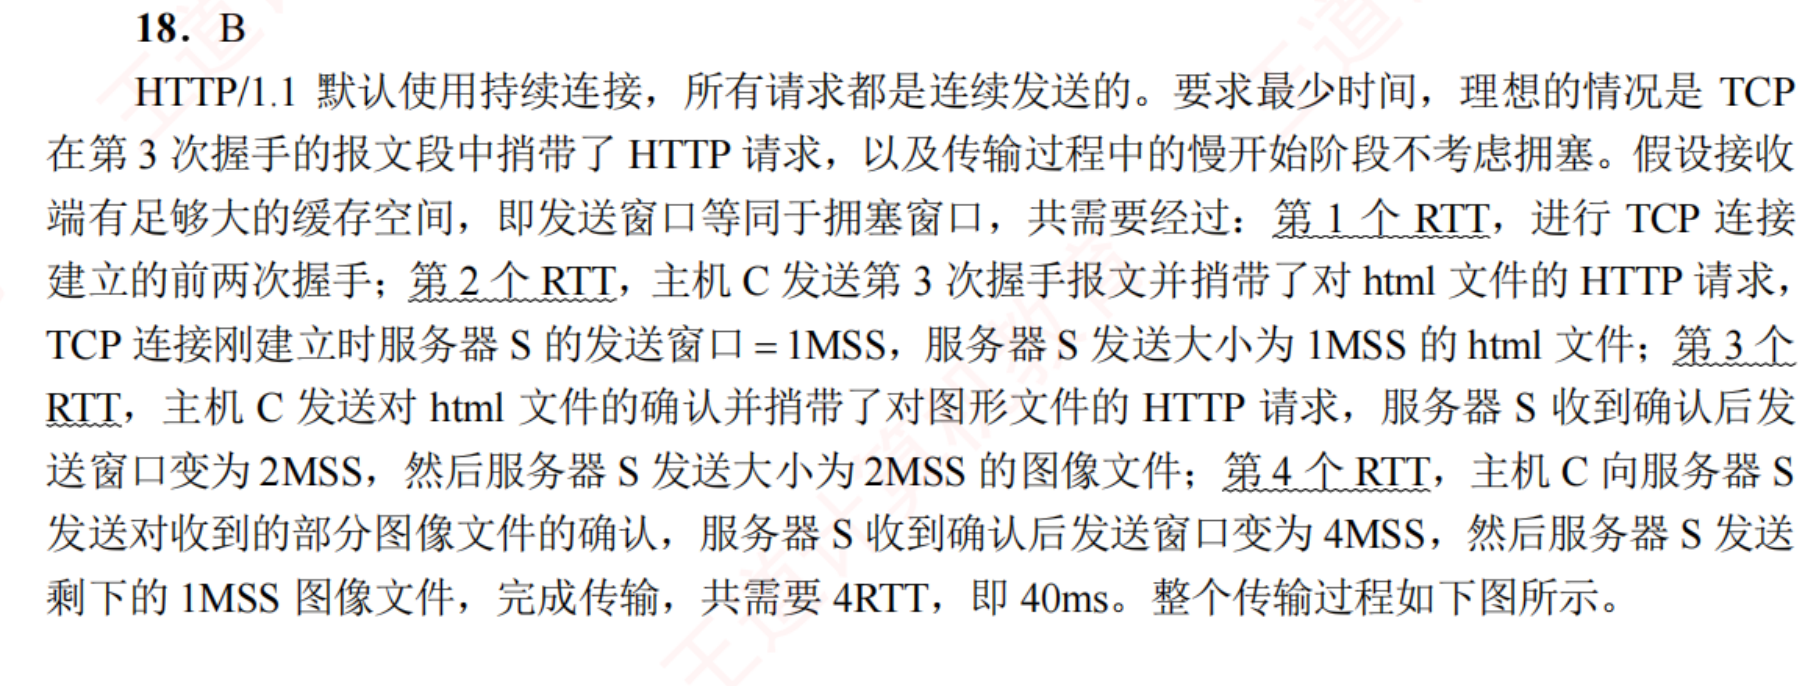
\includegraphics[width=161.13mm,height=180mm,keepaspectratio]{../solutions/assets/9e6cc86ca1bc2ca6f61587b1.png}\par\smallskip
\par\medskip\noindent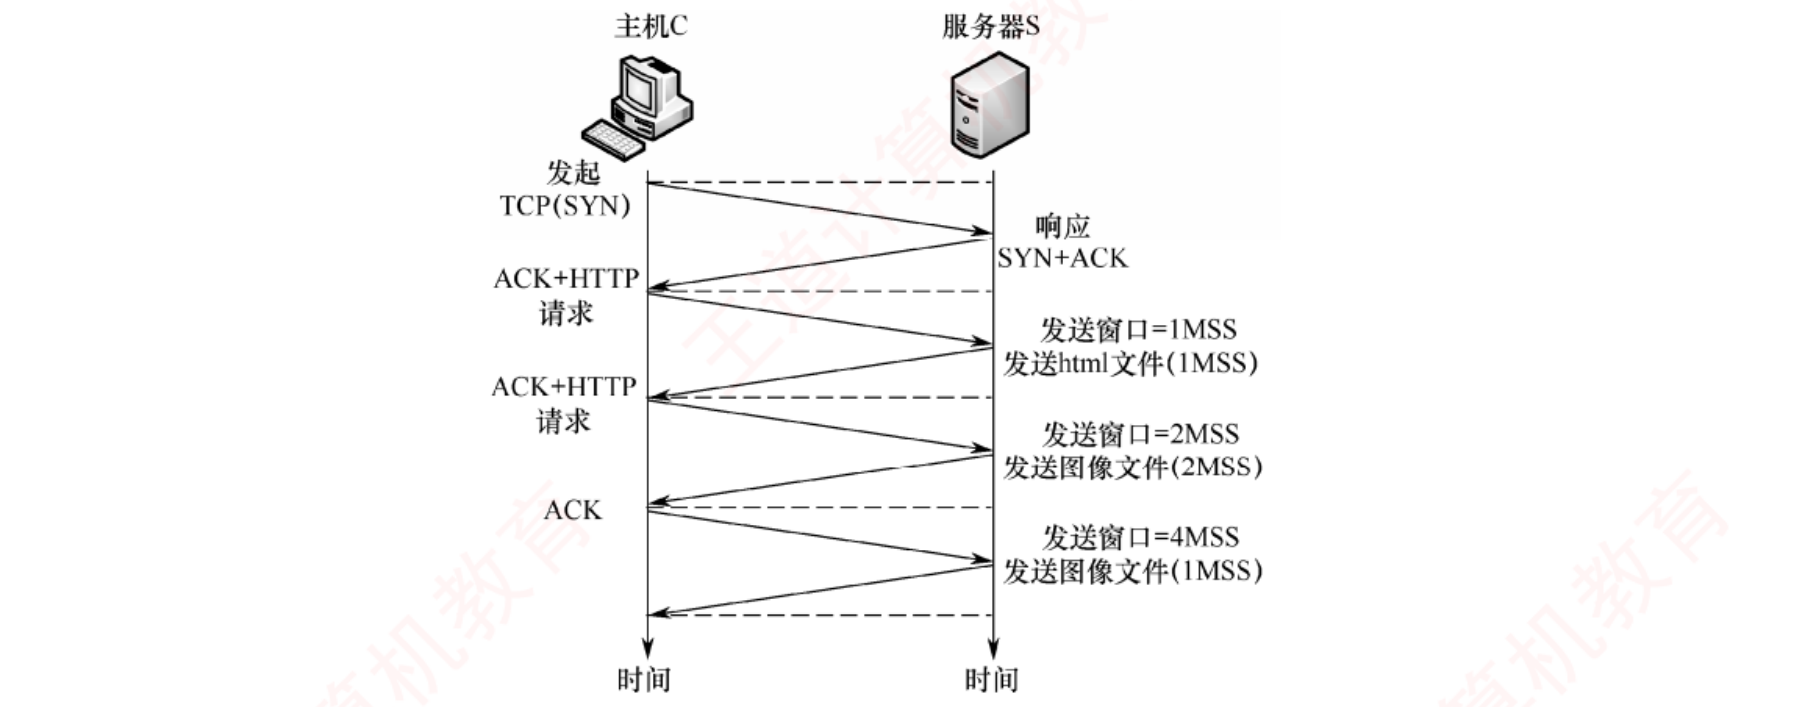
\includegraphics[width=161.13mm,height=180mm,keepaspectratio]{../solutions/assets/bac403dc24c15dc463edf18c.png}\par\smallskip
\par\medskip\Needspace{5\baselineskip}\noindent\hypertarget{a:CN06-E08}{}\label{a:CN06-E08}\textbf{例 6-8}\quad （1）控制持久、数据非持久，先建控制；（2）101、18102；（3）3 MSS、5 MSS；（4）60 ms、2.4 Mb/s。
\par\smallskip
先把FTP会话与一次文件传输分开。控制连接在整个FTP会话期间保持，承载登录、命令与控制信息，因此是\textbf{持久连接}；本题的数据连接服务于本次文件传输，传完后关闭，是\textbf{非持久连接}。登录时先建立的是\textbf{控制连接}，已经完成的登录过程不再计入第（4）问的数据连接计时。

数据连接的SYN占序号100，F首字节从\textbf{101}开始。18000 B文件占序号101～18100，发送完后H的FIN占18101，服务器第二次挥手的ACK应确认下一个期望序号，故为\textbf{18102}。这里确认的是文件数据再加FIN，不能把登录控制连接的序号混进来。

拥塞控制沿用教材的轮次模型：初始\(cwnd=1\) MSS，达到4 MSS门限后按每RTT增加1 MSS。先看ACK落在哪个时刻：确认号2101累计确认\(2101-101=2000\) B，即前2个段。第1个ACK使cwnd从1增为2 MSS；第2个ACK是第二轮中较早的那个，此时仍在慢开始，cwnd从2增为\textbf{3 MSS}。不能把``第二轮结束时4 MSS''提前用于这个ACK。

确认号7101累计确认\(7101-101=7000\) B，即\(1+2+4=7\)个段，恰好完成第3轮。此轮开始时已到4 MSS门限，采用拥塞避免，第3轮结束后窗口为\textbf{5 MSS}。下表同时列出数据发送、确认时刻与累计量，时间均从数据连接SYN发出算起。

\begin{longtable}[]{@{}lrrr@{}}
\toprule\noalign{}
阶段 & 开始时刻/ms & 本轮cwnd/MSS & 本轮发送段数 \\
\midrule\noalign{}
\endhead
\bottomrule\noalign{}
\endlastfoot
数据连接握手 & 0 & --- & --- \\
数据第1轮 & 10 & 1 & 1 \\
数据第2轮 & 20 & 2 & 2 \\
数据第3轮 & 30 & 4 & 4 \\
数据第4轮 & 40 & 5 & 5 \\
数据第5轮 & 50 & 6 & 6 \\
\end{longtable}

\begin{longtable}[]{@{}lrr@{}}
\toprule\noalign{}
阶段 & 累计发送段数 & 本轮全部确认到达/ms \\
\midrule\noalign{}
\endhead
\bottomrule\noalign{}
\endlastfoot
数据连接握手 & 0 & 10 \\
数据第1轮 & 1 & 20 \\
数据第2轮 & 3 & 30 \\
数据第3轮 & 7 & 40 \\
数据第4轮 & 12 & 50 \\
数据第5轮 & 18 & 60 \\
\end{longtable}

建立数据连接用1 RTT，18个段按1、2、4、5、6分5轮发完，并在最后一轮结束时得到全文件确认，所以总计\(6\mathrm{RTT}=\mathbf{60\ ms}\)。期间应用层平均速率为\(18000\times8/0.060=\mathbf{2.4\ Mb/s}\)，也就是300000 B/s=0.3 MB/s。分母按题目包含握手、不包含连接释放；不能只用50 ms的数据传输阶段，也不能因服务器较早收到最后一比特就省去最后确认的回程。

这里的按轮增长是题目采用的教材近似，阈值前逐ACK检查仍有意义；拥塞避免阶段不宜把轮次表误解成每个ACK都使cwnd增加整整1 MSS。若要描述某个操作系统的精确逐ACK轨迹，还需其拥塞算法和ACK策略。

\par\medskip\Needspace{5\baselineskip}\noindent\hypertarget{a:CN06-E09}{}\label{a:CN06-E09}\textbf{例 6-9}\quad （1）DNS，UDP/IP/以太网封装；（2）H1→4、DNS→1、R→2；（3）2帧，目的全FF（需新DNS查询）。
\par\smallskip
解题入口是按依赖关系列出``先知道谁的地址，才能发下一帧''。按本题及教材需要新做域名解析的流程，H1先运行\textbf{DNS}，把域名换成Web服务器IP；常规查询的封装为\textbf{DNS报文\ensuremath{\to}UDP数据报\ensuremath{\to}IPv4分组\ensuremath{\to}Ethernet II帧}。ARP用于在本地链路上解析MAC，不是DNS外面的一层，也不是另一个应用层协议；CSMA/CD是介质访问算法，不是帧格式，在全双工交换链路中通常不运行。

H1先根据\texttt{/25}判断本地DNS的192.168.1.126与自己同属192.168.1.0/25，先用ARP解析本地DNS的MAC地址，不先问网关。解析出Web服务器位于外网后，才ARP查询网关R的192.168.1.1。后续IP分组的最终目的仍是Web服务器，当前以太网帧的目的MAC却是R的MAC。

\begin{longtable}[]{@{}
  >{\raggedright\arraybackslash}p{(\columnwidth - 6\tabcolsep) * \real{0.2308}}
  >{\raggedright\arraybackslash}p{(\columnwidth - 6\tabcolsep) * \real{0.2308}}
  >{\raggedleft\arraybackslash}p{(\columnwidth - 6\tabcolsep) * \real{0.3077}}
  >{\raggedright\arraybackslash}p{(\columnwidth - 6\tabcolsep) * \real{0.2308}}@{}}
\toprule\noalign{}
\begin{minipage}[b]{\linewidth}\raggedright
顺序
\end{minipage} & \begin{minipage}[b]{\linewidth}\raggedright
S收到的帧
\end{minipage} & \begin{minipage}[b]{\linewidth}\raggedleft
入端口
\end{minipage} & \begin{minipage}[b]{\linewidth}\raggedright
S的处理与新增学习
\end{minipage} \\
\midrule\noalign{}
\endhead
\bottomrule\noalign{}
\endlastfoot
1 & H1广播ARP，询问本地DNS的MAC & 4 & 学习H1的cc\ensuremath{\to}4；向1、2、3口泛洪 \\
2 & DNS单播ARP应答给H1 & 1 & 学习DNS的bb\ensuremath{\to}1；已知cc，只转4口 \\
3 & H1单播DNS查询给DNS & 4 & 已知bb，只转1口 \\
4 & DNS单播查询应答给H1 & 1 & 已知cc，只转4口 \\
5 & H1广播ARP，询问网关R的MAC & 4 & 向1、2、3口泛洪 \\
6 & R单播ARP应答给H1 & 2 & 学习R的aa\ensuremath{\to}2；只转4口 \\
7 & H1向外网服务器发送TCP SYN，帧发给R & 4 & 已知aa，只转2口 \\
8 & R转发服务器的SYN+ACK，帧发给H1 & 2 & 已知cc，只转4口 \\
9 & H1发送TCP确认及首个HTTP请求 & 4 & 帧均发给R，只转2口；到达题设\(t_1\) \\
\end{longtable}

表中cc、bb、aa分别是下表完整MAC地址的末字节缩写。第三次握手ACK是否与首个HTTP请求合并，不改变学习或H2收到的帧数。交换机按\textbf{帧的源MAC与入端口}学习，不会从广播帧的目的地址、ARP询问目标、IP目的地址或题图上``知道有H2''便自行添加表项。因此\(t_1\)时为：

\begin{longtable}[]{@{}lr@{}}
\toprule\noalign{}
MAC地址 & 端口 \\
\midrule\noalign{}
\endhead
\bottomrule\noalign{}
\endlastfoot
00-11-22-33-44-cc（H1） & 4 \\
00-11-22-33-44-bb（本地DNS） & 1 \\
00-11-22-33-44-aa（R） & 2 \\
\end{longtable}

H2只被动收到两次广播ARP请求，没有发出自己的帧，故没有dd\ensuremath{\to}3条目。两次单播应答到来时，交换机早已从相应请求学到H1的位置，不会因初始表为空便把所有单播一直泛洪。第（3）问按上述解析流程，H2至少收到\textbf{2个ARP请求帧}，分别查询本地DNS和网关，目的MAC均为\textbf{FF-FF-FF-FF-FF-FF}。

这个2帧结论以本题意图中的新DNS查询为前提。原题明确为空的是ARP表和交换表，并未额外声明DNS缓存为空；若允许命中已有DNS缓存，就不必先访问本地DNS，相应学习表与最小广播数都会改变。应保留这一条件边界，不能把``通过域名访问''推广成任何情况下都必然重新发送DNS查询。

\end{document}